% Copyright (C) 2020-2024 by Thomas Auzinger <thomas@auzinger.name>

\PassOptionsToPackage{dvipsnames,table}{xcolor} % Ensure that the document loads packages with all required options.
\documentclass[draft,final]{istaustriathesis}

% Set the copyright license. The possible choices are 'restricted' to reserve all rights or a Creative Commons license.
% See https://creativecommons.org/choose/ for information on choosing a license.
% The supported Creative Commons licenses are 'cc-by', 'cc-by-sa', 'cc-by-nd', 'cc-by-nc', 'cc-by-nc-sa', and 'cc-by-nc-nd'.
\setlicense{restricted} % Choose 'restricted' or any of the 'cc-by...'.
% If a Creative Commons license is chosen, the corresponding license information can be added to the PDF metadata.
% For this, the package 'doclicense' needs to be uncommented below.
% Furthermore, the 'modifier' option of 'doclicense' needs to mirror the chosen Creative Commons license.
\usepackage[type={CC},modifier={by-nc-sa},version={4.0},hyperxmp=false]{doclicense} % Sets the license metadata. See copyright licensing below.
% If no Creative Commons license is chosen, then the appropriate copyright text and (potentially empty) URL must be entered manually.
% For this, edit the command \Copyright{...} and \CopyrightURL{...} in the filecontents* environment of \jobname.xmpdata below.

% The pdfx package throws an error when utilizing the \xspace command inside the XMP metadata generation.
% Since \xspace is utilized by the \doclicenseLongTextForHyperref command of the doclicense package, a workaround is implemented below.
% It defines a \doclicenseLongTextForHyperrefFixed command that can be used instead of \doclicenseLongTextForHyperref.
\begingroup
\renewcommand{\xspace}{\space} % Temporarily replace \xspace with \space.
\xdef\doclicenseLongTextForHyperrefFixed{\doclicenseLongTextForHyperref} % Expand the \doclicenseLongTextForHyperref and define the fixed version globally.
\endgroup

% Define convenience functions to use the author name and the thesis title in the PDF document properties.
\newcommand{\authorname}{Al Depope} % The author name without titles.
\newcommand{\displaythesistitle}{From Sparse Selection \\ to Risk Prediction: \\ Approximate Message Passing for \\ Proteomic Survival Models and Large-Scale Genomics}
\newcommand{\thesistitle}{From Sparse Selection to Risk Prediction: Approximate Message Passing for Proteomic Survival Models and Large-Scale Genomics}
% \newcommand{\thesistitle}{From Sparse Selection to Risk Prediction: Approximate Message Passing for Proteomics Survival Models and Large-Scale Genomics} % The title of the thesis.
\newcommand{\issn}{2663-337X} % Standard ISSN of all ISTA PhD theses.
% \newcommand{\isbn}{978-0-00000-000-0} % Leave empty if no ISBN is used.
\newcommand{\isbn}{} % Leave empty if no ISBN is used.
% Please contact IST Library library@ist.ac.at if you want to register an ISBN for your thesis.

\providecommand{\bmhead}[1]{\section*{#1}}

\setstocksize{240mm}{170mm}
\settrimmedsize{\stockheight}{\stockwidth}{*}
\setbinding{10mm} % Adds 1cm of "dead space" to the spine for the glue
\setlrmarginsandblock{15mm}{20mm}{*} % {inner}{outer}{ratio}
\setulmarginsandblock{25mm}{20mm}{*} % {top}{bottom}{ratio}
\checkandfixthelayout

% Approximate Message Passing for Biomarker Discovery and Prognosis in Proteomics Survival Models and Large-Scale Genomics
% From Sparse Selection to Risk Prediction: Approximate Message Passing for Proteomics Survival Models and Large-Scale Genomics
% Approximate Message Passing for Proteomics Survival Models and Large-Scale Genomics

% Create the XMP metadata file for the creation of PDF/A compatible documents.
\begin{filecontents*}[overwrite]{\jobname.xmpdata}
\Author{\authorname}                                    % The author's name in the document properties.
\Title{\thesistitle}                                    % The document's title in the document properties.
\Language{en-US}                                        % The document's language in the document properties. Select 'en-US' or 'en-GB'.
\Keywords{a\sep list\sep of\sep keywords}               % The document's keywords in the document properties (separated by '\sep ').
\Publisher{Institute of Science and Technology Austria} % The document's publisher in the document properties.
\Subject{PhD Thesis}                                    % The document's subject in the document properties.
\Copyright{\doclicenseLongTextForHyperrefFixed}         % The document's copyright message in the document properties.
\CopyrightURL{\doclicenseURL}                           % The document's copyright URL in the document properties.
\Copyrighted{True}
\ISBN{\isbn}                                            % The document's ISBN in the document properties.
\Journalnumber{\issn}                                   % The document's ISSN in the document properties.
\end{filecontents*}

% Extended LaTeX functionality is enabled by including packages with \usepackage{...}.
\usepackage{algorithmic}
\usepackage[english]{babel} % The language of the thesis. Use 'british' for British English.
\usepackage[numbers]{natbib} % Extend bibliography management. "numbers" matches the alpha labels ([DBMR26]); without it natbib stops with an error on repeated compiles.
\usepackage{nicematrix}
\usepackage{float}
\usepackage{bibentry}   % Provide full citation support for single references.
\usepackage{amsmath}    % Extended typesetting of mathematical expression.
\usepackage{amssymb}    % Provides a multitude of mathematical symbols.
\usepackage{mathtools}  % Further extensions of mathematical typesetting.
\usepackage{microtype}  % Small-scale typographic enhancements.
\usepackage[inline]{enumitem} % User control over the layout of lists (itemize, enumerate, description).
\usepackage{multirow}   % Allows table elements to span several rows.
\usepackage{booktabs}   % Improves the typesetting of tables.
\usepackage{subcaption} % Allows the use of subfigures and enables their referencing.
\usepackage[ruled,linesnumbered,algochapter]{algorithm2e} % Enables the writing of pseudo code.
\usepackage[dvipsnames,table]{xcolor} % Allows the definition and use of colors. This package has to be included before TikZ.
\usepackage{nag}        % Issues warnings when best practices in writing LaTeX documents are violated.
\usepackage{todonotes}  % Provides tooltip-like todo notes.
\usepackage{morewrites} % Increases the number of external files that can be used.
\usepackage{bm}
\usepackage{amsthm}
\usepackage{xurl}
\newtheorem{lemma}{Lemma}
\usepackage{caption}
% All captions in 10pt (\small inside a caption also gives 10pt), so that the long
% figure legends fit on the 170 x 240 mm page together with their figures.
\DeclareCaptionFont{thesisfootnotesize}{\footnotesize\let\small\footnotesize}
\captionsetup{font=thesisfootnotesize}
% Second half of a legend that continues on the next page (\ContinuedFloat):
% labelled "Figure 2.1 (continued):".
\DeclareCaptionLabelFormat{continued}{#1~#2 (continued)}

% Figure legend that can break across pages.  \caption always builds one
% unbreakable box, so a full-width graphic with a long legend has to shrink to
% keep both on the same page.  Here the legend is ordinary text instead: the
% graphic stays at full width and the legend runs on to the next page.
% Arguments: list-of-figures entry, legend, label.
\newcommand{\breakablefigurecaption}[3]{%
  \par\addvspace{\abovecaptionskip}%
  \refstepcounter{figure}\label{#3}%
  \addcontentsline{lof}{figure}{\protect\numberline{\thefigure}{#1}}%
  \begingroup\footnotesize\let\small\footnotesize
    \noindent\figurename~\thefigure: #2\par
  \endgroup
  \addvspace{\belowcaptionskip}\addvspace{\parskip}%
}

% Pseudocode that can break across pages (the construction first used for vampW):
% caption between two rules, the algorithmic lines as normal text, a closing rule.
% Arguments: list-of-algorithms entry, caption, label.
\newenvironment{breakablealgorithm}[3]{%
  \par\begingroup\vspace{1em}%
  \noindent\begin{minipage}{\textwidth}%
    \hrule height 0.8pt\vspace*{1pt}%
    \captionsetup{type=algocf, font=normalsize, labelfont=bf, labelsep=colon, textfont=normalfont, justification=justified, singlelinecheck=false, skip=0pt, aboveskip=0pt, belowskip=0pt, margin={1.0em, 0pt}}%
    \caption[#1]{#2}\label{#3}%
    \vspace*{1pt}\hrule height 0.8pt
  \end{minipage}\par
  \vspace*{2pt}%
  \begin{adjustwidth}{1.5em}{0pt}% indent the lines by 1.5em and narrow them accordingly
}{%
  \end{adjustwidth}%
  \par\nopagebreak\vspace*{2pt}\hrule height 0.8pt\vspace{1em}\endgroup
}
\usepackage{pdfpages}   % Inserts the front and back cover (graphics/covers/).
\usepackage[a-2b,mathxmp]{pdfx}  % Enables PDF/A compliance. Loads the package hyperref and has to be included second to last.
\usepackage[acronym,toc]{glossaries} % Enables the generation of glossaries and lists of acronyms. This package has to be included last.

% Set PDF document properties
\hypersetup{
	pdfpagelayout   = OneColumn,            % How the document is shown in PDF viewers (optional).
	linkbordercolor = {Melon},                 % The color of the borders of boxes around hyperlinks (optional).
}

\setpnumwidth{2.5em}        % Avoid overfull hboxes in the table of contents (see memoir manual).
\setlength{\cftbeforechapterskip}{0.6em plus 1pt} % Less space above chapter entries (memoir default 1em), so the table of contents fits on two pages instead of putting its last entry (Appendix D) alone on a third.
\setsecnumdepth{subsection} % Enumerate subsections.

\nonzeroparskip             % Create space between paragraphs (optional).
% Chapter/appendix number: memoir's veelo style puts it (18 mm tall) in the outer margin,
% where the wide letters A, B, C reach the trimmed page edge. Keep its size, but end it
% at the right edge of the text block, after "CHAPTER"/"APPENDIX".
\renewcommand*{\printchapternum}{\hspace{.3em}\resizebox{!}{\beforechapskip}{\chapnumfont\thechapter}}
\raggedbottom               % Leftover space on a page goes to the bottom (like a \vfill there) instead of stretching the gaps between paragraphs and headings.
\setlength{\parindent}{0pt} % Remove paragraph indentation (optional).
\setlength{\marginparwidth}{2cm} % Silences a todonotes warning; the thesis has no margin notes.
\setlength{\emergencystretch}{3em} % Lets TeX break difficult paragraphs in the narrow 125 mm column instead of overfilling a line.

\nobibliography* % Allow the use of full citation in the list of publications.

\makeindex      % Use an optional index.
\makeglossaries % Use an optional glossary.
%\glstocfalse   % Remove the glossaries from the table of contents.

% Comment the following line to switch the document to a serif font, i.e., Latin Modern Roman
% (see https://tug.org/FontCatalogue/latinmodernroman/)
% \renewcommand{\familydefault}{\sfdefault} % Switch document to sans serif font, i.e., Latin Modern Sans.
% (see https://tug.org/FontCatalogue/latinmodernsans/)

% Set the page numbers to bottom centered.
\makeevenfoot{plain}{}{\thepage}{} % For front and back matter.
\makeoddfoot{plain}{}{\thepage}{} % For front and back matter.
\makeevenfoot{Ruled}{}{\thepage}{} % For main matter.
\makeoddfoot{Ruled}{}{\thepage}{} % For main matter.

% Required data.
\setthesis{phd} % Select 'master' or 'phd'.
\settitle{\thesistitle}
\setsubtitle{} % Comment this line if no subtitle is used.
% If your subtitle contains commas, enclose it with additional curvy brackets (i.e., \setsubtitle{{subtitle text}}) or define it as a macro as done with \thesistitle.
\setdate{2026}{06}{26} % Set signing date with 3 arguments: {day}{month}{year}.
\setissn{\issn}
% \setisbn{\isbn} % Comment this line if no ISBN is used.

% Define convenience function for an ISTA affiliation.
\newcommand{\istaustriaaffiliation}{ISTA, Klosterneuburg, Austria}

% Set persons with 4 arguments:
%  {title(s) before name}{name}{title(s) after name}{affiliation}
%  where both titles are optional (i.e. can be given as empty brackets {}).
% Some of the following persons are optional for Master's or PhD theses and can be commented if they do not apply.
\setauthor{}{\authorname}{}{\istaustriaaffiliation}
\setsupervisor{}{Prof. Matthew R. Robinson}{}{\istaustriaaffiliation}
\setcosupervisor{}{Prof. Marco Mondelli}{}{\istaustriaaffiliation} % Optional for Master's and PhD theses.
\setcommitteememberI{}{Prof. Dan Alistarh}{}{\istaustriaaffiliation}
% \setcommitteememberII{}{Prof. Na Cai}{}{ETH Zurich, Zurich, Switzerland} % Optional for Master's thesis.
\setcommitteememberII{}{Prof. Philip Schniter}{}{The Ohio State University, Columbus, USA} % Optional for Master's and PhD theses.
%\setcommitteememberIIII{}{Name Surname}{}{Institution, Place, Country} % Optional for Master's and PhD theses.
\setdefensechair{}{Prof. Matthew Kwan}{}{\istaustriaaffiliation} % Optional for Master's thesis.


%------------------- Notation shortcuts -------------------------------%
\def\ba{{\boldsymbol a}}
\def\beps{{\boldsymbol \epsilon}}
\def\bA{{\boldsymbol A}}
\def\bI{{\boldsymbol I}}
\def\bSigma{{\boldsymbol \Sigma}}
\def\bO{{\boldsymbol O}}
\def\bD{{\boldsymbol D}}
\def\bQ{{\boldsymbol Q}}
\def\bLambda{{\boldsymbol \Lambda}}
\def\blambda{{\boldsymbol \lambda}}
\def\by{{\boldsymbol y}}
\def\bx{{\boldsymbol x}}
\def\bY{{\boldsymbol Y}}
\def\bX{{\boldsymbol X}}
\def\bW{{\boldsymbol W}}

\newcounter{suppnotegvamp}

% for vampW to work perfectly, the following commands need to be defined. They are used to keep track of the number of supplementary notes in the main text and to refer to them in the appendix.
\usepackage{booktabs}
\let\botrule\bottomrule
\DeclareOldFontCommand{\bf}{\normalfont\bfseries}{\mathbf}
\DeclareOldFontCommand{\rm}{\normalfont\rmfamily}{\mathrm}
\DeclareOldFontCommand{\it}{\normalfont\itshape}{\mathit}
\DeclareOldFontCommand{\sf}{\normalfont\sffamily}{\mathsf}
\DeclareOldFontCommand{\tt}{\normalfont\ttfamily}{\mathtt}
\DeclareMathOperator*{\argmax}{arg\,max}
% memoir's \changed{...} is a change-mark command that prints nothing unless change marks
% are switched on; the text wrapped in it (4 sentences in Chapter 3, legend of Figure C.8) must print.
\renewcommand{\changed}[1]{#1}

\begin{document}
%%%%%%%%%%%%%%%%%%%%%%%%%%%%%%%%%%%%%%%%%%%%%%%%%%%%%%%%%%%%%%%%%%%%%%%%%%%%%%%%%%%%%%%%%%%%%%%%%%%%
%%% FRONT MATTER %%%%%%%%%%%%%%%%%%%%%%%%%%%%%%%%%%%%%%%%%%%%%%%%%%%%%%%%%%%%%%%%%%%%%%%%%%%%%%%%%%%
%%%%%%%%%%%%%%%%%%%%%%%%%%%%%%%%%%%%%%%%%%%%%%%%%%%%%%%%%%%%%%%%%%%%%%%%%%%%%%%%%%%%%%%%%%%%%%%%%%%%
\frontmatter % Switch to roman page numbering and prevent chapter numbering.
\pagestyle{plain} % Set simple page numbering.
\pagenumbering{gobble}
% Front cover, followed by its blank inside page, so that the title page stays a
% right-hand (odd) page.
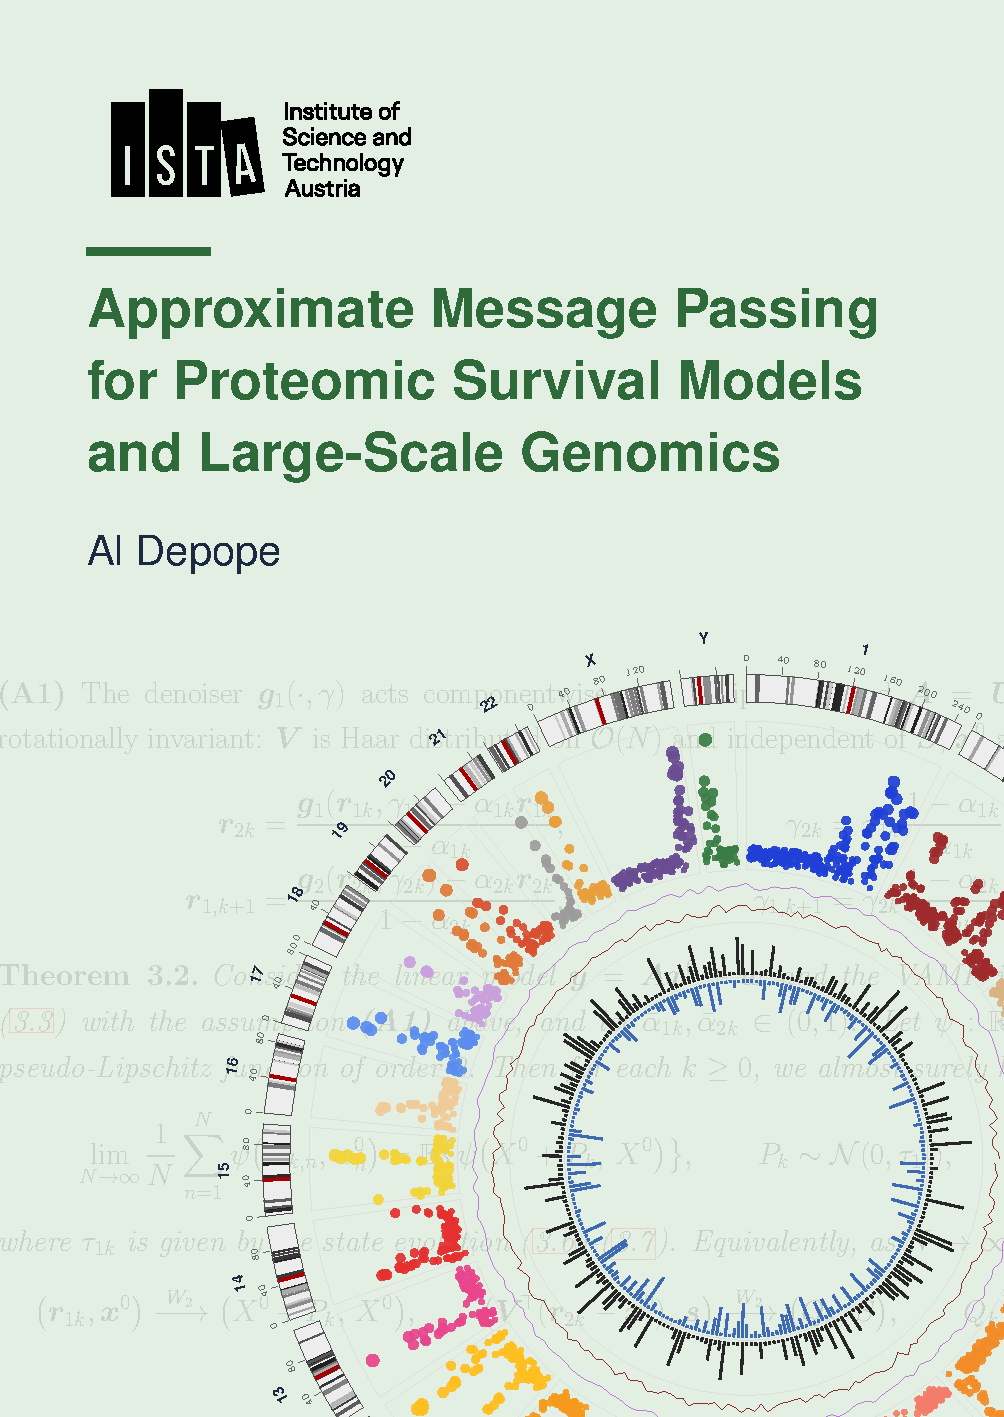
\includepdf[pages=1]{graphics/covers/front_light_green_170x240.pdf}
\begingroup\pagestyle{empty}\null\clearpage\endgroup
% The structure of the thesis has to conform to the guidelines at
%  https://phd.pages.ist.ac.at/student-resources/.

\settitle{\displaythesistitle}
% Title page scaled to the 170 x 240 mm page (about 81% of A4): every font size one
% step smaller, smaller vertical gaps and a 4 cm logo, so that it fits on one page.
% The title keeps the line breaks it had on A4.
\begingroup
\makeatletter
\renewcommand{\istaustriathesis@Huge}{\LARGE}
\renewcommand{\istaustriathesis@Large}{\large}
\renewcommand{\istaustriathesis@large}{\normalsize}
\setlength{\istaustriathesis@bigskipamount}{4ex}
\renewcommand{\istaustriathesis@graphics@logo}{\includegraphics[width=4cm]{ISTA_black_vector.pdf}}
\makeatother
\addtitlepage
\endgroup
\settitle{\thesistitle} 

\addcommitteepage
\addstatementpage

% \addtitlepage
% \addcommitteepage
% \addstatementpage

\pagenumbering{roman} % Start page numbering.
% single nucleotide polymorphisms (SNPs)
\begin{abstract}
% Uncovering the genetic architecture of complex traits and pinpointing causal molecular drivers require the ability to distinguish true signals from noise within massive, high-dimensional omics datasets. To extract meaningful biological insights from these datasets, such as identifying causal genetic variants and proteins, scalable and accurate inference methods are essential. To this end, this thesis develops novel Bayesian inference frameworks based on Vector Approximate Message Passing and demonstrates their effectiveness in the modeling of disease onset times and quantitative physical and clinical measures.

% First, we introduce gVAMP, a Bayesian framework tailored for Genome-Wide Association Studies that enables the joint modeling of quantitative complex traits across millions of genetic variants. gVAMP demonstrates superior accuracy in variable selection and out-of-sample polygenic risk prediction compared to state-of-the-art approaches. We model human height using 17 million whole-genome sequence variants from the UK Biobank, incorporating a vast number of rare variants and revealing novel associations. gVAMP achieves a prediction accuracy of approximately 46\% for human height, representing the highest reported performance for this trait to date. 

% Second, we present vampW, a Bayesian framework for survival analysis applied to proteomic data. By effectively handling right-censoring and complex protein dependencies within the UK Biobank Pharma Proteomics Project dataset, vampW identifies 219 protein associations across 24 disease outcomes, the majority of which are not among the top marginal discoveries. We further adjust protein levels for exponential age effects, yielding 1,308 associations and highlighting the sensitivity of the analysis to the chosen age-correction methodology. Finally, vampW improves upon the variable selection capabilities of the commonly used (penalized) variants of the Cox proportional hazards model and delivers state-of-the-art out-of-sample prediction of disease onset times.

% Collectively, these methods provide powerful tools for dissecting the genetic architecture of complex traits and the proteomic drivers of disease onset. Furthermore, by delivering accurate polygenic risk scores and precise predictions of onset times, this work advances the capabilities of personalized medicine and clinical risk stratification.

Uncovering the genetic architecture of complex traits and pinpointing causal molecular drivers require the ability to distinguish true signals from noise within massive, high-dimensional omics datasets. To extract meaningful biological insights from these datasets, such as identifying causal genetic variants and proteins, scalable and accurate inference methods are essential. To this end, this thesis develops novel Bayesian inference frameworks based on Vector Approximate Message Passing (VAMP) and demonstrates their effectiveness in modeling disease onset times, as well as quantitative physical and clinical measures.

First, we introduce gVAMP, a Bayesian framework tailored for genome-wide association studies that enables the joint modeling of quantitative complex traits across millions of genetic variants. gVAMP demonstrates superior accuracy in variable selection and out-of-sample polygenic risk prediction compared to state-of-the-art approaches. We model human height using 17 million whole-genome sequence variants from the UK Biobank, incorporating a vast number of rare variants and revealing novel associations. gVAMP achieves a prediction accuracy of approximately 46\% for human height, representing the highest reported performance for this trait to date.

Second, we present vampW, a Bayesian framework for survival analysis applied to proteomic data. By effectively handling right-censoring and complex protein dependencies within the UK Biobank Pharma Proteomics Project dataset, vampW identifies 219 protein associations across 24 disease outcomes, the majority of which are not among the top marginal discoveries. It improves upon the variable selection capabilities of the commonly used (penalized) variants of the Cox proportional hazards model and delivers state-of-the-art, out-of-sample prediction of disease onset times.

Collectively, these methods provide powerful tools for dissecting the genetic architecture of complex traits and the proteomic drivers of disease onset. Furthermore, by delivering accurate risk scores, this work advances the capabilities of personalized medicine and clinical risk stratification.

\end{abstract}

% The Acknowledgement chapter is optional and can be removed.
\begin{acknowledgements}
I would like to thank many people with whom I have scientifically and personally interacted
over the last five and a half years at the Institute. Firstly, I thank my supervisors, Matt Robinson and Marco Mondelli, 
for coming up with an interesting interdisciplinary project and giving me the opportunity to pursue it.
I also thank my lab colleagues for all the nice discussions, walks, and lunches. Finally, I want to thank Philip Schniter and Dan Alistarh for agreeing to join my thesis committee, and, together with Matthew Stephens, for providing fruitful feedback over the years.

There is also life outside of scientific work, and I would really like to thank the following people 
who have impacted my life in the most positive way over the past few years:
\begin{itemize}
\item Marta, my sister Nika, and my parents for always being there for me.
\item My late grandfather Frenki for his love and constant sense of pride in me, despite the fact that he did not understand most of the things I was working on.
% \item My other grandparents, Cecilija, Danica, and Miodrag, and my uncle Darko, for their continuous love and support.
\item My grandparents Cecilija, Danica, and Miodrag, and my uncle Darko, for their support.
\item Jakub and Ilse for all the inside jokes and brightening many of the days up.
\item Lucija, Borna, Lovro, and Dorotea for their friendship.
\end{itemize}
\bigskip\bigskip
% \section*{Funding acknowledgements}
% \vspace{5pt}
% This work was supported in part by the Swiss National Science Foundation through the Eccellenza Grant "Improving estimation and prediction of common complex disease risk" (grant number PCEGP3\_181181); the European Research Council through the grant "Inference in High Dimensions: Light-speed Algorithms and Information Limits" (grant number 101161364); and the Fondation Jean-Jacques et Felicia Lopez-Loreta through the Prix Lopez-Loretta 2019.
\end{acknowledgements}

\begin{aboutauthor}
% \todo[inline]{
	% Include paragraph of text summarizing your educational background, your academic profile (e.g. relevant research projects or work experience, list of publications), to give readers a snapshot idea of you as a person/academic.
	% It is not meant to be a CV in the sense that it is not intended for job applications.
	% This means things like your email address, your nationality, your current address, etc., should be left out.}
% \todo[inline,color=white]{
    Al Depope completed his BSc in Mathematics and MSc in Mathematical Statistics at the University of Zagreb before joining the Institute of Science and Technology Austria (ISTA) in September 2020. His primary research interests focus on the development of scalable inference methods and their applications in genomics and proteomics. During his doctoral studies, he developed the scientific software gVAMP, a high-dimensional tool capable of jointly analyzing millions of genetic variants. This work was published in Cell Genomics. Al has presented his research at international venues, including the ICASSP 2024 conference in South Korea and the European Mathematical Genetics Meeting 2024, where he received the Best Student Presentation Award. In his free time, he enjoys running and hiking.
	% Al Depope completed his BSc in Mathematics and MSc in Mathematical Statistics at the University of Zagreb before joining the Institute of Science and Technology Austria (ISTA) in September 2020. His primary research interests focus on the development of scalable inference methods and their applications in genomics. During his doctoral studies, alongside other projects, he developed the scientific software gVAMP, a high-dimensional tool capable of jointly analyzing millions of genetic variants. These findings were published in \textit{Cell Genomics}. Al has presented his research at international venues, including the ICASSP 2024 conference in South Korea and the European Mathematical Genetics Meeting, where he received the Best Student Presentation Award. In his free time, he enjoys running and hiking. %}
\end{aboutauthor}

\begin{publicationlist}  % Remove if not applicable for a Master's thesis.
% \todo[inline]{
% 	Specify all co-authors and collaborator contributions to this thesis.
% 	See the \href{https://phd.pages.ist.ac.at/graduate_school_guidelines_for_thesis_submission/}{Guidelines for Thesis Submission} for details.
% }
\begin{itemize}
    % \item \textbf{Chapter 2} is based on the following two publications, with only minor modifications in format and wording:
    
    \item \textbf{Chapter 2} is based on the following publication, with only minor modifications:

    % \begin{itemize}

        % \item 
        \bibentry{Depope2026}
        % Depope, A., Bajzik, J., Mondelli, M., and Robinson, M.R. (2026). Joint modeling of whole-genome sequencing data for human height via approximate message passing. Cell Genomics 6, doi: 10.1016/j.xgen.2026.101162.

        \vspace{5pt}   

        % \bibentry{depope_joint_2023} 
        in which MM and MRR conceived the study. AD, MM and MRR designed the study. AD derived the model and the algorithm, with input  from MM and MRR. AD wrote the software, with input from MM and MRR. AD, JB, MM, and MRR conducted the analysis and wrote the paper. All authors approved the final manuscript prior to submission. 

    % \end{itemize}

    % \item \textbf{Chapter 3} uses full preprint, with minor modifications of format and wording:
    
    % Jakub Bajzik*, Al Depope*, Yasaman Zolfimoselo, Alexander Sharipov, Holger Klein, Marco Mondelli, Matthew R. Robinson. Joint Variable Selection in Proteomics Survival Models, \textit{Preprint}, 2026. 
    % \vspace{5pt}   

    \item \textbf{Chapter 3} is based on the following manuscript, which has been accepted for the ICLR 2026 Workshop on Machine Learning for Genomics Explorations:
    
    \bibentry{bajzik2026joint}
    \vspace{5pt}   
    
    in which AD, MM and MRR conceived the study. AD, JB, MM and MRR designed the study. AD derived the model and the algorithm, with contributions from AS, JB, YZ, MM and MRR. JB, AD, and YZ prepared the data. JB, AD, YZ and AS wrote the software, and conducted the analyses. MM and MRR provided study oversight. JB, AD, MM and MRR wrote the paper. All authors approved the final manuscript prior to submission.
\end{itemize}

During his PhD, Al Depope also authored the following publication, which is not included in this thesis: 

\vspace{5pt}
% \item 
\bibentry{DepopeICASSP24}
    % \nocite{DepopeICASSP24}
    % A. Depope, M. Mondelli and M. R. Robinson, "Inference of Genetic Effects via Approximate Message Passing," ICASSP 2024 - 2024 IEEE International Conference on Acoustics, Speech and Signal Processing (ICASSP), Seoul, Korea, Republic of, 2024, pp. 13151-13155, doi: 10.1109/ICASSP48485.2024.10447198. 

    \vspace{5pt}    

    in which MM and MRR conceived the study. AD, MM and MRR designed the study. AD derived the model and the algorithm, with input  from MM and MRR. AD wrote the software, with input from MM and MRR. AD, MM, and MRR conducted the analysis and wrote the paper. All authors approved the final manuscript prior to submission. 

% \todo[inline,color=white]{
% 	Use the \texttt{\textbackslash bibentry} command to produce a full citation:
% }
% \bibentry{Turing1936} % Exemplary full citation.
\end{publicationlist}

\begin{ethicalstatement}
% % These projects were realized using UK Biobank data under project number 35520. UK Biobank genotypic and phenotypic data is available through a formal request at \url{http://www.ukbiobank.ac.uk}. The UK Biobank has ethics approval from the North West Multi-centre Research Ethics Committee (MREC). Methods were carried out in accordance with the relevant guidelines and regulations, with informed consent obtained from all participants. Informed consent for all All of Us participants is conducted in person or through an eConsent platform that includes primary consent, HIPAA Authorization for Research use of electronic health records and other external health data, and Consent for Return of Genomic Results. The protocol was reviewed by the Institutional Review Board (IRB) of the All of Us Research Program. The All of Us IRB follows the regulations and guidance of the NIH Office for Human Research Protections for all studies, ensuring that the rights and welfare of research participants are overseen and protected uniformly.
Projects presented in this thesis were realized utilizing data from the UK Biobank and the \textit{All of Us} Research Program. UK Biobank data was accessed under project number 35520, and its genotypic and phenotypic data are available through a formal request at \url{http://www.ukbiobank.ac.uk}. The UK Biobank has ethics approval from the North West Multi-centre Research Ethics Committee (MREC).

Across both datasets, all methods were carried out in accordance with the relevant guidelines and regulations, with informed consent obtained from all participants. Specifically, informed consent for all \textit{All of Us} participants is conducted in person or through an eConsent platform that includes primary consent, HIPAA Authorization for the research use of electronic health records and other external health data, and Consent for the Return of Genomic Results. The protocol was reviewed by the Institutional Review Board (IRB) of the \textit{All of Us} Research Program. The \textit{All of Us} IRB follows the regulations and guidance of the NIH Office for Human Research Protections for all studies, ensuring that the rights and welfare of research participants are overseen and protected uniformly.
\end{ethicalstatement}

\cleardoublepage
\renewcommand{\contentsname}{Table of Contents} % Specify chapter heading for table of contents.
\tableofcontents
\cleardoublepage
\listoffigures


% Create a group and deactivate all page breaks and blank pages.
% This puts the lists of figures, tables, etc. on the same pages.
% To reintroduce page breaks or blank pages, take the lists out of the group.
\begingroup % Starting a group keeps the deactivations restricted to the group.
\let\newpage\relax
\let\clearpage\relax
\let\cleardoublepage\relax

\listoftables
\listofalgorithms\addcontentsline{toc}{chapter}{List of Algorithms}
\printglossary[title={List of Terms}]
\printglossary[type=\acronymtype,title={List of Abbreviations}]
\endgroup % End the deactivation group.

%%%%%%%%%%%%%%%%%%%%%%%%%%%%%%%%%%%%%%%%%%%%%%%%%%%%%%%%%%%%%%%%%%%%%%%%%%%%%%%%%%%%%%%%%%%%%%%%%%%%
%%% MAIN MATTER %%%%%%%%%%%%%%%%%%%%%%%%%%%%%%%%%%%%%%%%%%%%%%%%%%%%%%%%%%%%%%%%%%%%%%%%%%%%%%%%%%%%
%%%%%%%%%%%%%%%%%%%%%%%%%%%%%%%%%%%%%%%%%%%%%%%%%%%%%%%%%%%%%%%%%%%%%%%%%%%%%%%%%%%%%%%%%%%%%%%%%%%%
\mainmatter % Switch to Arabic page and chapter numbering.
\pagestyle{Ruled} % Show chapter and section name at the top of the page.
%\pagestyle{plain} % Alternative page style without the names at the top.

\chapter{Introduction}

\section{Motivation}

Predicting disease risk and various health-related complex traits is a central goal of personalized preventative healthcare. This thesis uses two different types of biological information to create a clearer picture of a person's health state.

The first part of the work focuses on the inherited genetic information every person is born with. Because these data are massive and exhibit a complex structure, there is a need for efficient and accurate computational approaches to predict health-related traits directly from the DNA. These methods help estimate an individual's genetic predisposition for physical measurements, such as heel bone mineral density. They also extend to critical biomarkers, including blood cell counts, glycated hemoglobin, and lipid levels, alongside other physiological indicators.

The second part of this work moves beyond static genetics to develop approaches for analyzing plasma protein concentrations and their associations with clinical outcomes. The proteome is dynamic and fluctuates in response to aging and pathology, encoding a snapshot of an individual's physiological state at the moment of sampling. By capturing this snapshot, it is possible to model the timing distributions of disease onset and assess an individual's current health state more accurately.

The significance of the computational approaches presented here is twofold. First, they enable the identification of genetic variants and protein biomarkers associated with target phenotypes, which can lead to a better understanding of underlying biological mechanisms. Second, they facilitate the development of predictive models that can be used in clinical settings to identify individuals at high risk for certain diseases, allowing for early intervention and personalized treatment strategies.

In the following sections, we provide the necessary background for understanding these methods, starting with a short introduction to computational human genomics and proteomics, followed by a brief overview of commonly used statistical approaches for genome-wide association studies and survival modeling. Finally, we outline the foundational Approximate Message Passing framework that underpins our methods and precisely formulate the research questions this thesis answers.

\section{Population-scale genomics and proteomics}
\newacronym{snp}{SNP}{Single Nucleotide Polymorphism}
\subsection{Genomic fundamentals}

Deoxyribonucleic acid (DNA) is a double-helix molecule that carries the genetic instructions for life, composed of four chemical bases: adenine (A), cytosine (C), guanine (G), and thymine (T). \glspl{snp} represent variations at specific single-base positions within these sequences. Specifically, biallelic SNPs are defined by the substitution of one nucleotide for another at a given locus. Although the global reservoir of human genetic variation is immense, a typical individual genome contains approximately 4 million distinct SNPs \cite{1000Genomes2015}. Most of these variants are functionally neutral; however, a critical subset drives phenotypic variation, including susceptibility to disorders such as hypertension and schizophrenia. These complex traits characteristically result from the collective impact of hundreds or thousands of individual SNPs \cite{visscher201710}.

In the context of human heredity, biallelic SNPs are inherited biparentally, meaning each individual possesses two alleles per SNP, one of maternal origin and one of paternal origin. An allele is defined as one of the specific variant forms of a DNA sequence located at a given locus. Given this diploid nature, the genotypic state is efficiently encoded by counting the number of copies of the alternative allele. Typically, this alternative allele corresponds to the minor allele, which is the variant less prevalent in the cohort, while the reference allele represents the major or more common variant. This results in a discrete additive encoding that takes values in $\{0, 1, 2\}$, where 0 indicates zero copies of the alternative allele, 1 indicates a heterozygous state (one copy of each), and 2 indicates two copies of the alternative allele.
% This results in a discrete additive encoding that takes values in $\{0, 1, 2\}$: $0$ denotes homozygosity for the reference allele, $1$ denotes heterozygosity, and $2$ denotes homozygosity for the alternative allele. 
Since this ternary state requires only two bits of memory per variant and maximizes the number of zero entries, such an approach is highly efficient. It is widely adopted for large-scale genotype data, most notably in the PLINK binary file format \cite{purcell2007plink}, which leverages this bit-level packing to optimize both storage efficiency and computational scalability.

\newacronym{ukb}{UKB}{UK Biobank}
\newacronym{wgs}{WGS}{Whole-Genome Sequencing}
\subsection{Biobank-scale genomics}

The \gls{ukb} \cite{Bycroft2018} is a biomedical database comprising pseudonymized genetic and phenotypic data from approximately half a million individuals. These volunteers were enrolled at various assessment centers across the United Kingdom. Upon enrollment, biological samples were collected for DNA extraction and subsequent genotyping, while their ongoing health outcomes continue to be monitored via linkage to electronic health records. The primary mission of this repository is to enable research into the genetic and environmental factors underlying human diseases, with the goal of advancing clinical diagnostics, preventative care, and targeted therapeutics.

% Volunteers, aged 40 to 69 at recruitment, were enrolled at various assessment centers across the United Kingdom. Upon enrollment, biological samples were collected from which their DNA was extracted and genotyped, while their health outcomes continue to be monitored via linkage to electronic health records. The primary mission of this repository is to enable research into the genetic and environmental factors underlying human diseases, with the goal of advancing clinical diagnostics, preventative care, and targeted therapeutics.

% Upon enrollment, their DNA was collected and subsequently genotyped, while their health outcomes continue to be monitored via linkage to electronic health records. The core mission of this repository is to enable research into the genetic and environmental factors underlying human diseases, with the ultimate goal of advancing clinical prevention, diagnostics, and therapeutics.

% This resource was established with the primary objective of facilitating the investigation of genetic and environmental determinants of disease, thereby improving prevention, diagnosis, and treatment for a wide range of illnesses. 

The development of high-throughput, second-generation whole-genome sequencing technologies has enabled the characterization of genetic variation across billions of positions in the human genome. Within the UKB cohort, genetic profiling has evolved from initial genotyping arrays toward increasingly comprehensive sequencing. Specifically, Whole-Exome Sequencing (WES) \cite{VanHout2020,Szustakowski2021,Backman2021} targets the exome---roughly 1-3\% of the genome \cite{exome_coverage,UkBiobank_WGS2025}---which contains the protein-coding regions where many high-impact functional mutations are concentrated.
% Specifically, Whole-Exome Sequencing (WES) \cite{VanHout2020,Szustakowski2021,Backman2021} targets the protein-coding regions---roughly 1-2\% of the genome---where many high-impact functional mutations are concentrated. 
However, the most complete resolution is provided by \gls{wgs} \cite{UkBiobank_WGS2025}, which captures the entirety of the approximately 3 billion base pairs that constitute the human reference genome. This exhaustive coverage facilitates the discovery of rare variants and structural changes, including variation in critical non-coding regions such as enhancers and promoters. Most recently, the eight-year UKB Whole-Genome Sequencing Project reached completion, with its 2025 publication reporting that while each individual genome is approximately 3 billion bases long, a total of 1.1 billion unique variant sites were identified across 500,000 participants \cite{UkBiobank_WGS2025}.

\subsection{Rare variants}

A significant portion of these variants are rare---many occurring in only a small number of individuals within the cohort. With the cataloging of common variation largely saturated by decades of traditional array-based research, the immense catalog of novel variants captured by WGS consists almost entirely of rare and ultra-rare variants \cite{UkBiobank_WGS2025}.

However, this scarcity underscores a fundamental statistical challenge posed by limited sample sizes, which persists even in the world's most extensive biobanks. For instance, the UK Biobank, with its 500,000 participants, or other major initiatives like the \textit{All of Us Research Program} \cite{allofus} that target around 1 million individuals, still often lack the necessary sample sizes for robust, independent statistical inference of every variant. Furthermore, testing over a billion variants individually introduces an extreme multiple-testing burden. 

To mitigate this, a typical approach is to perform a preliminary filtering step to retain only variants observed in at least a certain number of individuals (e.g., a minor allele count of 20 or 30), which, after the quality control, reduces the dataset to the order of magnitude of tens of millions of SNPs and indels \cite{Wainschtein2026}. Alternatively, researchers frequently employ aggregation strategies, such as burden tests \cite{weighted_sum_test}, which collapse multiple rare variants within a functional unit into a single statistical score, or variance-component tests \cite{SKAT}.

However, understanding the true architecture of these traits requires evaluating these rare variants individually, as evolutionary genetics predicts a strong inverse relationship between a variant's allele frequency in a population and its effect size \cite{Schoech2019}. Variants that exert large, deleterious phenotypic effects are subject to strong purifying selection, which actively prevents them from becoming common. Consequently, the individual genetic variants with the most severe biological impacts are inherently rare. The aggregate impact of these large-effect rare variants is widely hypothesized to account for a significant portion of the "missing heritability" observed in complex traits \cite{missingHeritability2009, Zuk2014,Wainschtein2026}. This concept refers to the unresolved gap between the high genetic heritability of traits as estimated by family and twin-studies, and the relatively small fraction of that heritability that all known common variants can collectively explain.

To formalize this relationship between minor allele frequency and effect size, statistical frameworks model the expected variance of effect sizes as a power-law function of minor allele frequencies $(f_j)_{j=1}^{P}$, where $P$ is the total number of variants considered. In \cite{speed2017reevaluation}, this is modelled as $\mathbb{E}[\beta_j^2] \propto [f_j(1-f_j)]^{1+\alpha}$, where $\beta_j \in \mathbb{R}$ is a random variable describing the linear effect that variant $j$ exerts on the phenotype of interest. By evaluating 42 human traits, this framework demonstrated that an estimated parameter of $\alpha \approx -0.25$ yields a higher model likelihood than the traditional baseline of $\alpha = -1$ (which assumes constant effect size variance regardless of minor allele frequency). This result implies that common SNPs account for a substantially larger proportion of overall heritability than previous estimates had suggested. Furthermore, incorporating this relationship has been shown to improve association testing performance \cite{hof2024ldak}.

\newacronym{ld}{LD}{Linkage Disequilibrium}

\subsection{Linkage disequilibrium}

The human genome is organized into chromosomes that are inherited from each parent as discrete, intact units. During meiosis, a process of recombination occurs, whereby the maternal and paternal chromosomes exchange segments. However, because these crossover events are finite, genetic variants in close physical proximity on the same chromosome are less likely to be separated. Consequently, these neighboring alleles tend to be inherited together more frequently than would be expected by chance---a phenomenon known as \gls{ld}.

This non-random association creates a dense correlation structure across the genome that generally decays as the physical distance between variants increases \cite{PRITCHARD20011}. A non-causal variant may exhibit a strong statistical signal simply because it is in high LD with the true underlying causal variant. Accounting for this correlation structure is essential, as failing to do so can lead to the misidentification of the biological drivers of a trait. A more detailed discussion of the statistical approaches used to resolve these causal signals is provided in Section \ref{sec:fine_mapping}.

\newacronym{ukb_ppp}{UKB-PPP}{UK Biobank Pharma Proteomics Project}
\subsection{The Plasma Proteome in UK Biobank}

The UKB has recently expanded its resources beyond genomic data to include comprehensive proteomics through the \gls{ukb_ppp} \cite{sun_plasma_2023}. Formed by a collaborative group of 13 biopharmaceutical companies, this initiative aims to map the plasma proteome—the comprehensive collection of proteins present in circulating blood. While DNA contains the static genetic instructions, plasma proteins are the dynamic functional molecules that carry out biological processes. Consequently, measuring the concentrations of these proteins provides a functional snapshot of the body's physiological state, bridging the gap between an individual's genetic risk and their actual health outcomes. This biological link is critical for clinical applications such as drug discovery. By mapping how genetic variants influence protein abundance, researchers can identify and validate therapeutic targets. Furthermore, these proteins serve as powerful biomarkers for predicting disease onset or progression long before symptoms appear.
The initial Phase 1 release of the UKB-PPP dataset offers proteomic profiles for approximately 54,000 participants and measures the relative abundance of roughly 2,900 unique proteins. The cohort for this phase was strategically constructed to maximize statistical power. It includes a randomly selected baseline set of participants to represent the general population alongside a targeted group of individuals with specific health outcomes of high interest to the consortium partners.

% with significantly higher precision
\newacronym{icd}{ICD}{International Classification of Diseases}
\subsection{Phenotypic information in UK Biobank}
To bridge the gap between molecular variation and clinical outcomes, the UKB links genomic and proteomic data to Electronic Health Records (EHRs), where diagnoses are standardized using \acrshort{icd}-9 and \acrshort{icd}-10 codes. This integration---combined with extensive physical measurements, biomarker assays, and questionnaires from baseline assessment centers---allows for the analysis of diverse phenotypic categories. These range from quantitative traits (e.g., standing height or cholesterol levels) to time-to-event outcomes derived from cancer and death registries, such as Alzheimer's age of onset or cancer survival times. The resource also includes a number of covariates—such as age, sex, assessment center location, and genetic principal components (PCs)—that are crucial for controlling population stratification and other confounding factors in association analyses.

\newacronym{gwas}{GWAS}{Genome-Wide Association Studies}

\section{Common statistical approaches for genome-wide association studies}

The primary objective of \gls{gwas} is to identify statistical associations between complex phenotypes and specific genetic variants, predominantly SNPs. In practice, a standard GWAS begins with precise phenotyping and large-scale genotyping, followed by quality control to mitigate biases and exclude unreliable variants. Researchers typically impute unmeasured variants into this cleaned dataset to maximize genomic coverage. Associations are subsequently evaluated across the genome using covariate-adjusted regression models (see Sections \ref{subsec:marginal_testing} and \ref{subsec:LOCO} for more details). Finally, to account for the massive multiple-testing burden, any implicated loci must meet strict Bonferroni-corrected significance thresholds and be validated in independent cohorts.

\subsection{Marginal association testing}
\label{subsec:marginal_testing}
In GWAS, marginal association testing is part of a standard approach to identify individual genetic variants associated with a target phenotype \cite{Sesia2021}. This method evaluates each SNP independently, typically fitting a model to test the null hypothesis that the effect size associated with SNP $j$ is zero, i.e., \( H_0: \beta_j = 0 \), against the alternative $H_1: \beta_j \neq 0$.

For continuous phenotypes (e.g., standing height, cholesterol levels), the association of the \(j\)-th SNP with the vector describing the phenotype of interest $\bm{y} \in \mathbb{R}^N$ is typically assessed using linear regression. To control for confounding factors such as macroscopic population structure or non-genomic variables, a matrix of covariates \( \bm{C} \in \mathbb{R}^{N \times C} \) (e.g., age, sex, and principal components) is included:
\begin{equation}
\bm{y} = \mu \bm{1}_N + \bm{g}_j \beta_j + \bm{C}\bm{\gamma} + \bm{\epsilon},
\end{equation}
% where $\mu \in \mathbb{R}$ is the intercept, $\bm{1}_N$ is an $N$-dimensional vector of ones, with $N$ representing the total number of individuals in the analysis, $\bm{g}_j \in \mathbb{R}^N$ is a vector of encoded genotype information for SNP $j$, \( \beta_j \) represents the effect size of variant $j$, $\bm{\gamma} \in \mathbb{R}^C$ is the vector of effect sizes related to the covariates, and \( \bm{\epsilon} \in \mathbb{R}^N \) is the error term, typically assumed to follow a Gaussian distribution. 
where $\mu \in \mathbb{R}$ is the unknown intercept, $\bm{1}_N$ is an $N$-dimensional vector of ones, with $N$ representing
the total number of individuals in the analysis, $\bm{g}_j \in \mathbb{R}^N$ is the known vector of encoded genotype information for SNP $j$, and $\beta_j$ represents the parameter of interest (the effect size of variant $j$). The vector $\bm{\gamma} \in \mathbb{R}^C$ contains the unknown fixed-effect sizes related to the observed covariates, where $C \ll N$ in typical GWAS settings. Finally, $\bm{\epsilon} \in \mathbb{R}^N$ is the unobserved random error term, typically assumed to follow a multivariate Gaussian distribution with a scaled-identity covariance matrix, $\bm{\epsilon} \sim \mathcal{N}(0, {\sigma_{\varepsilon}}^2 \bm{I}_N)$, where the residual variance ${\sigma_{\varepsilon}}^2$ is unknown. The notation $\mathcal{N}(\cdot, \bm{\mu}, \bm{\Sigma})$ denotes the normal distribution with mean vector $\bm{\mu}$ and covariance matrix $\bm{\Sigma}$. This marginal assessment often serves as a preliminary screening step. To disentangle true causal effects from correlations arising via linkage disequilibrium, these results are typically post-processed using clumping algorithms to isolate independent signals or Bayesian fine-mapping approaches to assign posterior causal probabilities to specific variants within an associated region. These probabilities can then be summed to form credible sets on the basis of a specified coverage probability threshold \cite{FineMapping2018}.

\newacronym{loco}{LOCO}{Leave-One-Chromosome-Out}
\newacronym{lmm}{LMM}{Linear Mixed Model}
\newacronym{grm}{GRM}{Genetic Relationship Matrix}

\subsection{Leave-One-Chromosome-Out association testing}
\label{subsec:LOCO}
A more refined approach to association testing involves the use of linear mixed models (LMMs) to account for familial relatedness and complex population structure \cite{Listgarten2012, mlma}. The standard LMM evaluates the association of a single candidate SNP using the following formulation:
% \begin{equation}
%     \bm{y} = \bm{X}_j \beta_j + \bm{g} + \bm{\epsilon}.
% \end{equation}
\begin{equation}
    \bm{y} = \bm{x}^{(j)} \beta_j + \bm{g} + \bm{\epsilon}.
\end{equation}
% Here, $\bm{y} \in \mathbb{R}^N$ represents the vector of phenotypes, % $\bm{X}_j \in \mathbb{R}^N$ 
% $\bm{x}^{(j)} \in \mathbb{R}^N$ is the genotype vector for the tested SNP indexed by $j$, $\beta_j$ is the fixed effect size of SNP $j$, $\bm{g}$ is the random polygenic effect, and $\bm{\epsilon}$ is the residual error. The random effect is typically assumed to be distributed as $\bm{g} \sim \mathcal{N}(\bm{0}, \bm{K} \sigma_g^2)$, where $\bm{K}$ is the global Genetic Relationship Matrix (GRM) constructed from all genome-wide SNPs, and $\sigma_g^2$ is the additive genetic variance. 
Here, $\bm{y} \in \mathbb{R}^N$ represents the vector of phenotypes, $\bm{x}^{(j)} \in \mathbb{R}^N$ is the known genotype vector for the tested SNP indexed by $j$, $\beta_j$ is the fixed effect size of SNP $j$, $\bm{g}$ is the random polygenic effect, and $\bm{\epsilon}$ is the residual error. The random effect is typically assumed to be distributed as $\bm{g} \sim \mathcal{N}(\bm{0}, \bm{K} \sigma_g^2)$, where $\bm{K}$ is the known global Genetic Relationship Matrix (GRM), which stores correlation information between individuals and is constructed from all genome-wide SNPs, and $\sigma_g^2$ is the unknown additive genetic variance. However, if the genomic region containing the tested SNP $j$ is included in the computation of the GRM, it leads to a phenomenon known as "proximal contamination" \cite{Listgarten2012}. Because of local linkage disequilibrium, the random effect $\bm{g}$ "absorbs" part of the candidate SNP's true fixed-effect signal. This double-fitting artificially deflates the test statistic and reduces statistical power. To circumvent this, modern GWAS tools employ a \gls{loco} strategy. In this approach, the association of each SNP on chromosome $c$ is evaluated while conditioning on a genetic background calculated from all other chromosomes:
% \begin{equation}
%     \bm{y} = \bm{X}_j \beta_j + \bm{g}_{-c} + \bm{\epsilon}.
% \end{equation}
\begin{equation}
    \bm{y} = \bm{x}^{(j)} \beta_j + \bm{g}_{-c} + \bm{\epsilon}.
\end{equation}
In this formulation, the polygenic effect $\bm{g}_{-c}$ is distributed as $\bm{g}_{-c} \sim \mathcal{N}(\bm{0}, \bm{K}_{-c} \sigma_{g,-c}^2)$, where $\bm{K}_{-c}$ is the GRM constructed strictly from markers outside of chromosome $c$. While traditional methods relied on computing and inverting massive $N \times N$ covariance matrices, modern and highly scalable frameworks often bypass the explicit calculation of $\bm{K}_{-c}$. Instead of modeling the background as a Gaussian variance component, these methods estimate a matrix-free LOCO polygenic predictor, $\bm{\hat{y}}_{-c}$, which is subsequently included as a fixed covariate or offset in the marginal regression:
% \begin{equation}
%     \bm{y} = \bm{X}_j \beta_j + \bm{\hat{y}}_{-c} + \bm{\epsilon}.
% \end{equation}
\begin{equation}
    \bm{y} = \bm{x}^{(j)} \beta_j + \bm{\hat{y}}_{-c} + \bm{\epsilon}.
\end{equation}
This approach preserves the strict LOCO rule by effectively eliminating local confounding and preventing the double-counting of genetic effects while achieving the computational efficiency required for biobank-scale cohorts.
Despite these advantages, the LOCO assumptions employed by modern LMMs and whole-genome regression methods can be broken by the presence of interchromosomal LD. When a truly associated candidate SNP is highly correlated with a variant on a different chromosome, the standard LOCO approach fails to isolate the signal. Because the distant correlated variant is kept in the background null model, it absorbs some or all of the fixed-effect signal during the computation of phenotypic residuals, leading to a distinct loss of statistical power ~\cite{regenie}.

While many tools are available to detect genetic associations \cite{bolt,fastGWA2019,SAIGE, regenie, hof2024ldak}, we focus on two common approaches here that will be used for benchmarking in Chapter \ref{ch:gvamp}. We detail REGENIE \cite{regenie} as a standard framework for mixed-model association analysis and the recent LDAK-KVIK \cite{hof2024ldak} method. Both are specifically designed to efficiently handle computations at the biobank scale.

REGENIE is an individual-level whole-genome regression framework built upon a stacked regression approach. It constructs the genetic predictors in two steps: First, it partitions the entire genome into contiguous blocks and fits a ridge regression model within each block to compute local polygenic predictions. Second, it uses these block-level predictions as variables in a global ridge regression. In this way, REGENIE implicitly models the sample-relatedness covariance structure and bypasses the calculation and exact inversion of the GRM. 

LDAK-KVIK is an individual-level, mixed-model association analysis tool that models the polygenic background using an elastic net prior, combining both Gaussian and Laplace penalties for SNP effects. The pipeline begins by testing the data for underlying genetic structure. It then estimates the power-law parameter $\alpha$ and total heritability via randomized Haseman-Elston regression, using these estimates to determine the heritability contributed by each individual SNP. It uses cross-validation to optimize the elastic net hyperparameters, fits the regression model using a variational Bayes approach, and constructs LOCO predictors for each chromosome. Furthermore, guided by the initial structure test, it scales the test statistics and executes the single-SNP association analysis.

We conclude this section by illustrating a key limitation of marginal association testing. Although such an approach is highly efficient for large-scale data, its failure to account for complex linkage disequilibrium leads to an overestimate of putative causal variants. These challenges necessitate the use of fine-mapping methods---approaches designed to disentangle true causal signals from the surrounding noise of correlated variants, typically in local regions. In Figure \ref{fig:fine_mapping_main_figure}a, we illustrate a scenario where two causal variants (red) are in high LD with a non-causal variant (blue). All mentioned variants exhibit significant marginal associations, but only the red ones are truly causal. Relying solely on a standard ranking of marginal associations fails to properly distinguish between causal and non-causal variants in this example. In contrast, Figure \ref{fig:fine_mapping_main_figure}b depicts posterior inclusion probabilities that can be used to construct credible sets (CS 1 and CS 2) with guaranteed false discovery control. 

\newacronym[longplural={Posterior Inclusion Probabilities}]{pip}{PIP}{Posterior Inclusion Probability}
\newacronym{rfr}{RFR}{Replication Failure Rate}
\newacronym{fdr}{FDR}{False Discovery Rate}
\newacronym{ibss}{IBSS}{Iterative Bayesian Stepwise Selection}

\begin{figure}[htbp]
    \centering
    \captionsetup[subfigure]{position=top, justification=raggedright, singlelinecheck=false}
    
    \begin{subfigure}{0.45\textwidth}
        \caption{}
        \centering
        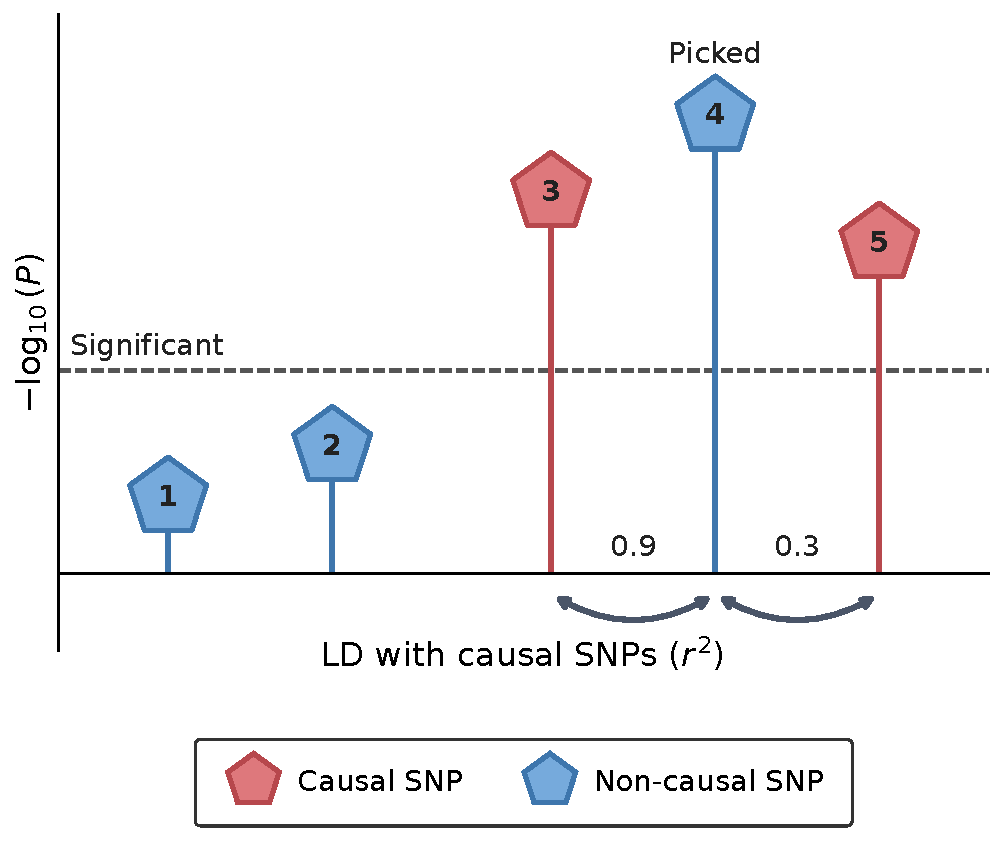
\includegraphics[width=\textwidth]{graphics/background_figures/ld_causal_plot.pdf}
        \label{fig:sub1}
    \end{subfigure}%
    \hfill
    \begin{subfigure}{0.45\textwidth}
        \caption{}
        \centering
        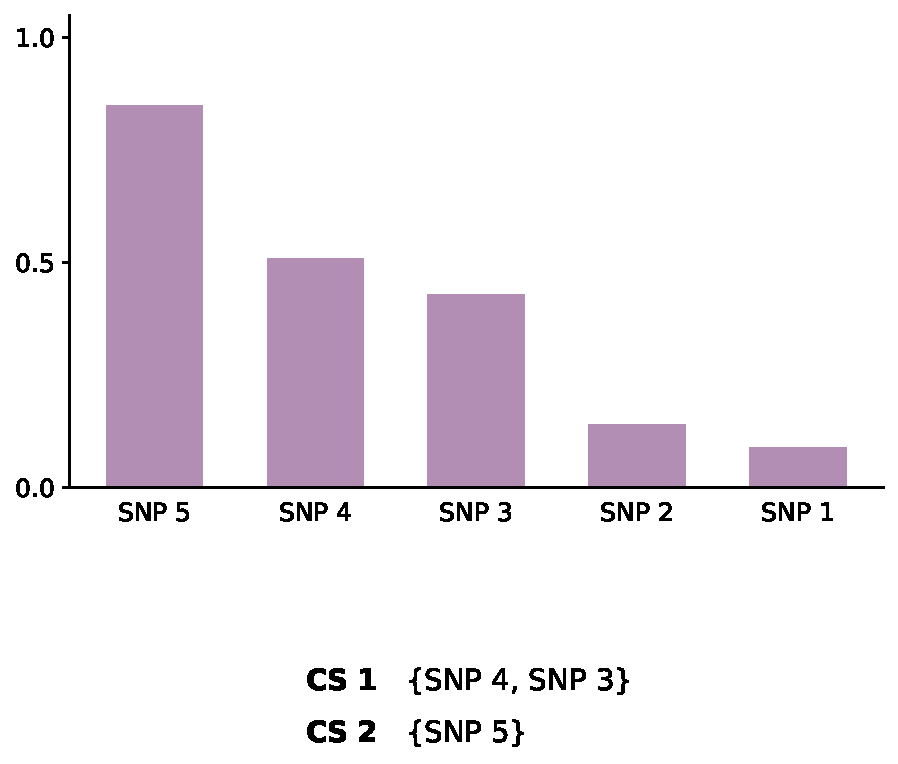
\includegraphics[width=\textwidth]{graphics/background_figures/fine_mapping_plot.pdf}
        \label{fig:sub2}
    \end{subfigure}
    
    \caption[Conceptual overview of the fine-mapping process highlighting the limitations of marginal association testing influenced by LD structure]{Conceptual overview of the fine-mapping process highlighting the limitations of marginal association testing influenced by LD structure. (a) Example of the correlation structure between causal and non-causal variants. The $y$-axis displays the significance of the marginal association testing. This example demonstrates that relying solely on a standard ranking of marginal associations fails to properly distinguish between causal and non-causal variants due to linkage disequilibrium. (b) The desired outcome of fine-mapping methods is the derivation of posterior inclusion probabilities for individual SNPs. These probabilities can then be used to construct credible sets (CS 1 and CS 2) with guaranteed false discovery control. This figure is adapted from \cite{FineMappingReview2025}.}
    \label{fig:fine_mapping_main_figure}
\end{figure}


\subsection{Statistical fine-mapping of genetic associations}

\label{sec:fine_mapping}

Building upon the preliminary screening provided by marginal association analyses, statistical fine-mapping aims to identify the causal genetic variants, typically within a local genomic window of length 1 Mb (one million base pairs). Overlapping windows are merged into a final set of loci ready for analysis \cite{FineMappingReview2025}. While the multiple regression framework serves as the foundation for these analyses, the primary challenge involves exploring the $2^P$ possible causal configurations within an associated locus containing $P$ genetic variants. To navigate this, fine-mapping methods are predominantly based on a Bayesian framework, which allows for incorporating prior assumptions about the genetic architecture of the trait, such as the expected number of causal variants per genomic window or the distribution of effect sizes that can further enhance the statistical power \cite{infinitesimalFineMapping2024}. Furthermore, such approaches can quantify probabilistic evidence in terms of \glspl{pip}, which can then be used to create disjoint credible sets. We define the \textit{$\alpha$-level credible set} as the minimal set of genetic variants that contains at least one causal variant with probability greater than or equal to $\alpha$. If we further define Bayesian FDR (bFDR) as the expected fraction of false discoveries under the posterior distribution of the model, then the following relationship holds between PIPs and bFDR (the proof of which can be found in Appendix \ref{Background_Appendix}):

\begin{lemma}[Bound on the Bayesian False Discovery Rate, adapted from \cite{Muller2004}]
Let $D$ be the observed GWAS data and $\mathcal{S}$ be a non-empty set of genetic variants selected as putative discoveries, with cardinality $|\mathcal{S}| > 0$. For every $j\in \mathcal{S}$, let $z_j \in \{0, 1\}$ be the unobserved, true causal indicator for variant $j$, and let $\text{PIP}_j = \mathbb{P}(z_j = 1 \mid D)$ be its PIP. Denoting the Bayesian False Discovery Rate of the set $\mathcal{S}$ as bFDR$(\mathcal{S})$, the following holds:

If there exists a constant $c \in [0, 1]$ such that $\text{PIP}_j \ge c$ for all variants $j \in \mathcal{S}$, then bFDR$(\mathcal{S}) \le 1 - c$.
\end{lemma}

Furthermore, it can be shown that to minimize posterior expected false negatives while strictly keeping the posterior expected false discovery proportion below a target threshold, the optimal decision rule is to rank and select all variants with a PIP above an appropriate threshold \cite{Muller2004}. Motivated by these results, we say a fine-mapping method is \textit{well-calibrated} if applying the thresholding rule $\text{PIP} \ge c$ guarantees that the observed \gls{fdr} is less than or equal to $1 - c$. In practice, the threshold $c = 0.95$ (yielding an observed $\text{FDR} \le 0.05$) is of primary interest.

Widely used frameworks for fine-mapping utilize different strategies to identify causal signals while maintaining computational efficiency:
\begin{itemize}
    \item Shotgun Stochastic Search with complexity reduction: Utilized by tools such as FINEMAP \cite{10.1093/bioinformatics/btw018}, this approach reduces the complexity of fitting a maximum likelihood estimator for a given configuration of hypothesized causal SNPs. Instead of scaling cubically with the total number of input SNPs, the complexity is reduced to cubic in the maximum number of hypothesized causal variants. This iterative procedure explores the search space by adding, deleting, or swapping a SNP within the current set at each step, enabling the identification of multiple causal signals per locus far more efficiently than exhaustive search methods.
    \item Sum of Single Effects (SuSiE) \cite{susie_original}: This framework reformulates the multiple regression model by expressing total genetic effects as a sum of a fixed number of single effects, where each component represents exactly one causal variant. The specific variable responsible for determining the location of each single effect is drawn from a multinomial distribution (typically uniform across all variants), while its non-zero coefficient is assumed to follow a normal distribution. The algorithm requires the user to input the maximum number of effects, while hyperparameters such as the residual Gaussian variance and prior effect variances are typically estimated directly from the data using an empirical Bayes approach that maximizes the variational evidence lower bound. This re-parameterization allows for Iterative Bayesian Stepwise Selection, a variational Bayes algorithm that avoids the need to search all possible SNP combinations. SuSiE offers linear computational complexity relative to the number of individuals and variants. More recent extensions of the SuSiE framework focus on using summary data \cite{susie} as the input to the algorithm and on fine-mapping multiple traits simultaneously \cite{SusieMultiTrait2026}.
\end{itemize}

One extension of the aforementioned approaches involves directly modeling background signals alongside SuSiE or FINEMAP via an infinitesimal model. Namely, standard fine-mapping frameworks usually assume strict sparsity, meaning that only a small number of variants causally contribute to the phenotype, and that all true causal signals are either included in, or highly tagged by, this sparse subset. However, failing to account for widespread and nonsparse genetic effects can lead to the miscalibration of posterior probabilities \cite{infinitesimalFineMapping2024}. To address this, methods such as SuSiE-Inf and FINEMAP-Inf \cite{infinitesimalFineMapping2024} explicitly incorporate an infinitesimal model alongside the sparse components, with a prior assuming that all variants contribute to the trait with equal variance. This combined architecture demonstrates superior calibration and tighter control over the replication failure rate, which serves as an approximate lower bound for the FDR. Additionally, one can further enhance the resolution of such analyses by integrating functional annotations, which provide prior information regarding the biological relevance of specific variants (e.g., coding changes or regulatory activity) \cite{FineMappingReview2025}. 

However, the scalability of these methods remains a critical bottleneck. Standard fine-mapping is typically performed locally, segmenting the genome into discrete, mostly independent LD blocks (e.g., 1--3 Mb regions) to make computation feasible. While this approach is sufficient for sparse genotyping arrays, the advent of whole-genome sequencing (WGS) within large-scale biobanks (e.g., UK Biobank, All of Us) presents a new challenge. In WGS settings, the density of variants increases dramatically, meaning that a single window may contain tens of thousands of variants. Moreover, this localized segmentation fundamentally fails to account for long-range LD. 

\newacronym{prs}{PRS}{Polygenic Risk Scores}
\newacronym{mcmc}{MCMC}{Markov chain Monte Carlo}
\section{Construction of polygenic risk scores}

\gls{prs} are quantitative measures that aggregate the effects of multiple genetic variants across the genome to estimate an individual's genetic predisposition to a particular trait or disease. The construction of PRS typically involves two main steps: (1) estimating the effect sizes of SNPs from GWAS summary statistics or individual-level data, and (2) aggregating these effects into a single score for each individual. The score for individual $i$ in the case of linear models is computed as
% The aggregation for individual $j$ in the case of linear models is computed as 
\begin{equation}
    \text{PRS}_i = \sum_{j=1}^{P} \hat{\beta}_j X_{i,j},
\end{equation}
where $\hat{\beta}_j$ is the estimated effect size of SNP $j$, $X_{i,j}$ is the known (column-normalized) genetic information of individual $i$ at SNP $j$, and $P$ is the total number of considered SNPs. Many of the commonly used methods for estimation of the effect sizes $\hat{\beta}_j$ are based on \gls{mcmc} sampling or variational Bayes inference. While MCMC offers asymptotically exact posterior distributions through stochastic sampling, it remains computationally demanding even when highly optimized; in contrast, variational Bayes approximates the posterior via deterministic optimization, trading a degree of theoretical exactness for gains in speed and scalability. Both frameworks yield PIPs that can also be used to construct credible sets of putative causal variants. In recent work \cite{Wu2024}, a genome-wide fine-mapping framework jointly leveraging functional genomic data was shown to outperform region-specific approaches, yielding more reliable causal variant identification and improved prediction across ancestry groups.

% In fact, recent work \cite{Wu2024} suggests that genome-wide fine-mapping approaches that integrate functional annotations can outperform earlier fine-mapping strategies, showing better calibration of posterior inclusion probabilities together with improved increased power and cross-ancestry predictive performance.

% In fact, recent work \cite{Wu2024} has shown that genome-wide fine-mapping with functional annotations improves over previously mentioned fine-mapping methods across multiple metrics including calibration of PIP values, mapping resolution, mapping precision, replication rate, and trans-ancestry phenotype prediction.

\subsection{Summary-level PRS methods}

\label{subsec:summary_level_prs}

\begin{figure}[htbp]
    \centering
    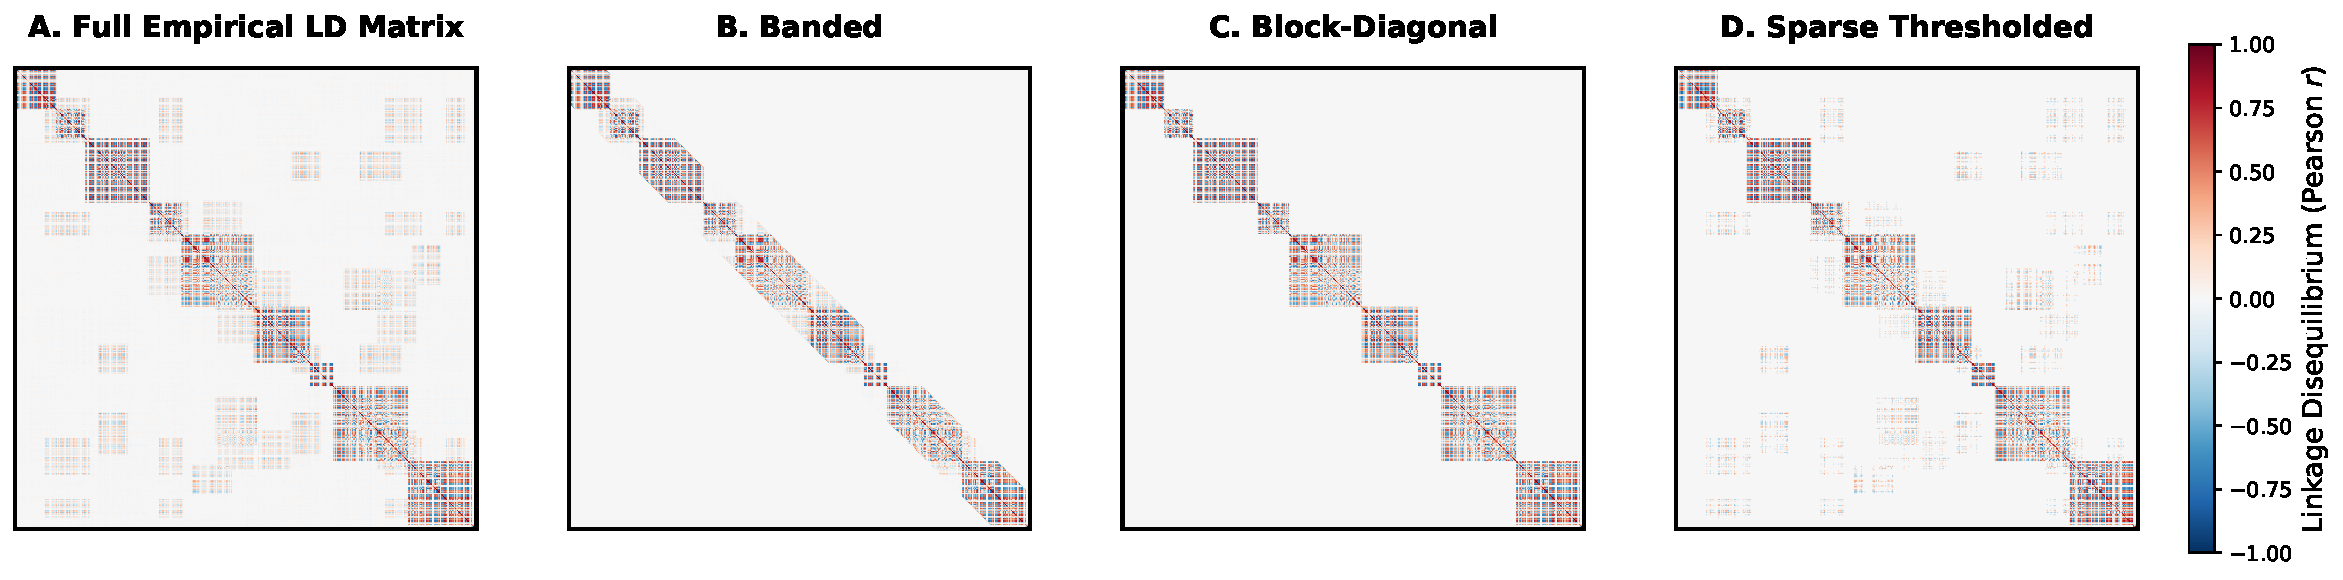
\includegraphics[width=\textwidth]{graphics/background_figures/ld_approximations_final.pdf}    
    \caption[Visual comparison of common LD matrix approximations]{\textbf{Visual comparison of common LD matrix approximations.} This figure illustrates the structure of an LD matrix within a single chromosome, as interchromosomal LD is conventionally assumed to be negligible. 
    \textbf{(A)} A full empirical LD matrix (Pearson correlation, $r$), showing dense local block structures alongside diffuse polygenic background correlations and complex longer-range LD signals. 
    \textbf{(B)} A banded approximation (e.g., utilized in LDpred models), where all correlations outside a strict bandwidth are set to zero. 
    \textbf{(C)} A block-diagonal approximation (e.g., utilized in SBayesR), where the genome is partitioned into independent LD blocks and all off-block correlations are set to zero. 
    \textbf{(D)} A sparse thresholded approximation, where all absolute correlations below a specified threshold are set to zero. While this approach preserves strong longer-range LD, it discards diffuse background correlations. Similar to the approximation errors introduced by matrix truncations, the zero inter-chromosomal LD assumption introduces further error.
    % Similar to the approximation errors introduced by these matrix truncations, assuming interchromosomal LD to be zero introduces further error. 
    This assumption is the main difference between models operating on full individual-level data and those relying on LD matrices and marginal effect sizes.}
    \label{fig:ld_approximations_final}
\end{figure}

Summary-statistic methods for constructing PRS utilize widely available GWAS summary statistics, which include marginal effect size estimates and their standard errors for each SNP, without requiring access to individual-level genotype data. They typically incorporate an external reference panel to account for the LD structure of the genome. Because the full genome-wide LD matrix is computationally intractable to store and invert, these methods rely on structural approximations---such as banded, block-diagonal, or sparse thresholded representations---to make inference feasible (Figure \ref{fig:ld_approximations_final}). Most modern implementations employ penalized regression techniques \cite{lassosum2017} or Bayesian frameworks to efficiently estimate effect sizes using either MCMC \cite{ldpred,sbayesr} or variational inference \cite{VIPRS2023,megaprs2021} approaches. In the remainder of this section, we give an overview of two widely used methods based on an MCMC approach: LDpred2 and SBayesR.

LDpred2 \cite{ldpred} is a Bayesian summary-level method that assumes a point-normal mixture prior for SNP effect sizes. Specifically, a learnable fraction of SNPs (treated as a hyperparameter) is assumed to be causal and assigned a Gaussian prior with equal variance across all causal variants, while the remaining non-causal variants have an effect size of exactly zero. LDpred2 employs a Gibbs sampler to estimate the posterior mean of the effect sizes. Its "auto" version bypasses the need for a validation dataset by estimating the fraction of causal SNPs and total heritability directly from the training data during the sampling iterations. The algorithmic time complexity scales linearly with the number of variants $P$, the number of Gibbs sampler iterations $N_{\text{it}}$, and the average number of variants within the window after an initial LD matrix pre-computation. Furthermore, the software utilizes a sparse matrix memory-mapping implementation in C++, which strictly bounds memory usage.

SBayesR \cite{sbayesr} is a summary-data-based multiple regression model that accommodates the varying degrees of polygenicity and effect size magnitudes inherent in complex traits. It generalizes the point-normal mixture prior of LDpred2 by utilizing a finite mixture of $L$ normal distributions combined with a point mass at zero, defined by the Dirac delta $\delta_0$, for the SNP effect sizes. The prior distribution for the effect $\beta_j$ of the $j$-th SNP is defined as:
\begin{equation}
\beta_j \sim (1-\lambda) \cdot \delta_0 + \lambda \cdot \sum_{l=1}^{L} \pi_l \cdot \mathcal{N}(\cdot, 0, \gamma_l \cdot \sigma_{\beta}^2),
\end{equation}
where $\lambda \in [0,1]$ is the sparsity rate, $(\pi_l)_{l=1}^L$ are the mixing probabilities of a causal SNP belonging to component $l=1,\dots,L$, $(\gamma_l)_{l=1}^L$ define the variance scaling factors.
%  and $\mathcal{N}(\cdot, \mu, \sigma^2)$ denotes the normal distribution with mean $\mu$ and variance $\sigma^2$. 
SBayesR operates with three non-spike components ($L=3$) whose variances form a geometric series with a factor of $10$. Posterior effects are estimated via a Gibbs sampler whose computational complexity scales linearly with the number of variants, the number of iterations, and the expected number of non-zero effects per iteration. This efficiency is achieved by exploiting a sparse representation of the LD structure and strictly updating only the non-zero effects during each iteration. 
% , the average number of non-zero elements per column in the LD matrix
\subsection{Individual-level PRS methods}

Individual-level inference methods for the construction of polygenic risk scores operate directly on genotype matrices rather than relying on aggregated summary statistics. By utilizing the complete genetic profile of each participant, these models can capture long-range correlation patterns between SNPs. However, this approach typically demands substantial computational resources and vast memory storage, especially as modern biobanks scale to hundreds of thousands of individuals. Additionally, strict data privacy regulations often restrict access to raw individual-level genotypes, making these methods less practical to the broader research community compared to methods that only require public summary statistics. 

Similar to the summary-level methods, most implementations employ penalized regression techniques \cite{snpnet2020,regenie} or Bayesian frameworks to efficiently estimate effect sizes using MCMC approaches \cite{BayesAB2010, BayesC2011, BayesRR2013, BayesR2015, Orliac2022}.

\subsection{Genetic architecture and predictive limits of complex traits}

The predictive accuracy of polygenic risk score methods is constrained by the genetic architecture of the target trait \cite{Chatterjee}. Here, genetic architecture refers to the underlying pattern of genetic contributions to a phenotype, including how many loci are involved, how large their effects are, and how those effects are distributed across the genome. Genetic architectures are often described as monogenic, oligogenic, or polygenic, depending on whether one, a few, or very many variants contribute to phenotypic variation \cite{genetic_architecture}. For traits with an oligogenic architecture, where a small set of variants has relatively large effects, standard regression or Bayesian approaches can readily identify the causal signals, allowing accurate prediction even from comparatively modest sample sizes. By contrast, for highly polygenic or omnigenic traits, genetic liability is spread over tens of thousands of variants, each with an almost negligible effect. In this setting, separating these tiny effects from sampling noise typically requires large, biobank-scale cohorts \cite{Chatterjee}. Moreover, because conventional PRS models are linear and additive, any variance arising from non-additive genetic components (such as dominance or epistasis) or from intricate gene-environment interactions is, by construction, outside their predictive scope. Traits such as standing height and body mass index are commonly used as exemplary traits in complex trait genetics, as they are among the most heritable, straightforward to measure, and strongly polygenic \cite{HTbig}.

Our understanding of the genomic regions underlying these traits has advanced considerably. Recent large-scale analyses, such as the association study of 5.4 million individuals of different ancestries by Yengo et al. \cite{HTbig}, have identified 12,111 independent SNPs significantly associated with height, collectively accounting for nearly all the common SNP-based heritability. These SNPs are concentrated in genomic segments spanning about 21\% of the genome. Providing a theoretical basis for such widespread genomic involvement, complementary research \cite{omnigenic} demonstrates that height is influenced by an extraordinarily large number of causal variants, each with a tiny effect size. Because these variants are spread so widely that almost every 100kb window contributes to the phenotypic variance, these findings strongly support the omnigenic model. Under this model, thousands of peripheral genes contribute to a phenotype by propagating regulatory effects through a few core biological pathways.

For highly polygenic traits such as height and BMI, most of the genetic signal lies not in protein-coding regions, but in non-coding regulatory elements that weakly modulate overall gene expression \cite{bmi_noncoding,yengo_meta-analysis_2018}. Driven by massive sample sizes, modern PRS methods have also made substantial progress in out-of-sample prediction accuracy for those traits. For standing height, state-of-the-art predictors report explaining up to 44.7\% \cite{HTbig} of the phenotypic variance in independent test cohorts of European ancestry. For BMI, where environmental and behavioral confounding is stronger, reported out-of-sample predictive accuracy plateaus at 17.6\% \cite{bmi_prs} of the phenotypic variance, as predicted using genetic data of around 5.1 million people. Unlike highly polygenic anthropometric traits, cardiometabolic traits like blood pressure and HbA1c yield significantly fewer independent associated loci, reflecting a sparser detectable genetic architecture where fewer regions achieve genome-wide significance (Table \ref{table:table2}).

For human height, 60\% to 80\% of the phenotypic variance in European ancestry is likely to be genetic \cite{missing_heritability_ht}, with a pedigree-based estimate of heritability reaching even 0.882 \cite{Wainschtein2026}. Whole-genome sequencing now estimates heritability at about 71\% using SNPs \cite{Wainschtein2026}. The genetic architecture of this captured variance is highly stratified: common variants drive 66\% of the pedigree-based heritability (compared to 14\% from rare variants), and non-coding regions contribute 80\% of the WGS-based heritability estimate (compared to 20\% from coding regions). The 20\% "missing" fraction of the total heritability is hypothesized to arise from ultra-rare (minor allele frequency $<0.001$) and structural variants not well tagged by SNPs, or non-additive genetic effects. 

To estimate the heritability parameter in whole-genome sequence data, researchers often rely on GREML-LDMS \cite{missing_heritability_ht}, which utilizes variance-component models to assess the aggregate contribution of different groups of variants. While successful in quantifying overall variance, this approach inherently requires stratifying variants based on allele frequency and linkage disequilibrium. In contrast, the gVAMP algorithm introduced in Chapter \ref{ch:gvamp} performs a joint analysis of rare and common variants within a unified, high-dimensional framework. By estimating the effect sizes of rare variants conditionally upon the common genetic background, gVAMP provides a methodology for both quantifying the variance attributable to rare variation at a much higher resolution and for effectively fine-mapping the underlying causal loci.

\section{Survival analysis}
Survival analysis provides a statistical framework for analyzing time-to-event or age-at-diagnoses data, characterized by the presence of censoring. While censoring can take several forms---such as left-censoring, where the event is known to have occurred prior to observation time, and right-censoring, where the study ends or the patient drops out before the event occurs---clinical data in the UK Biobank are predominantly right-censored. Hence, let the random variables $T$ and $C$ denote the true survival time and the censoring time, respectively. The observed data for individual $i$ consists of the pair $(t_i, \delta_i)$, where $t_i = \min(T_i, C_i)$ is the observed time and $\delta_i = \mathbb{I}(T_i \leq C_i)$ is the event indicator. The central object of interest is the hazard function $h(t)$, defined as the instantaneous rate of occurrence of the event at time $t$, conditional on the individual not having experienced the event until that time:

\begin{equation}
    h(t) = \lim_{\Delta t \to 0} \frac{P(t \le T < t + \Delta t \mid T \ge t)}{\Delta t}.
\end{equation}

\newacronym{coxph}{CoxPH}{Cox Proportional Hazards}
\subsection{Cox Proportional Hazards model}
The \gls{coxph} model \cite{coxPH1972} is a semi-parametric regression model that relates the hazard function for individual $i$ to a vector of covariates $\bm{x}_i \in \mathbb{R}^P$. The model assumes that the hazard for individual $i$ at time $t$ is the product of an unspecified baseline hazard $h_0(t)$ and an exponential multiplicative factor determined by the covariates:

\begin{equation}
    h(t \mid \bm{x}_i) = h_0(t) \exp(\bm{\beta}^\top \bm{x}_i),
\end{equation}

where $\bm{\beta} \in \mathbb{R}^P$ is a vector of regression coefficients, and $P$ is the number of covariates included in the study. Inference is typically performed by maximizing the partial likelihood $L(\bm{\beta})$, which eliminates the parameter $h_0(t)$. The partial likelihood is given by:

\begin{equation}
    L(\bm{\beta}) = \prod_{i: \delta_i = 1} \frac{\exp(\bm{\beta}^\top \bm{x}_i)}{\sum_{j \in \mathcal{R}(t_i)} \exp(\bm{\beta}^\top \bm{x}_j)},
\end{equation}

where $\mathcal{R}(t_i) = \{j : t_j \ge t_i\}$ represents the risk set (the set of individuals still at risk of experiencing the event) at time $t_i$. In practice, the log-partial likelihood, $\ell(\bm{\beta}) = \log L(\bm{\beta})$, is maximized due to its numerical properties. Importantly, the negative log-partial likelihood, $-\ell(\bm{\beta})$, is strictly convex with respect to $\bm{\beta}$, provided the covariate matrix is of full rank. While there is no closed-form analytical solution for the estimator $\hat{\bm{\beta}}$, this strict convexity guarantees a unique global minimum for the negative log-partial likelihood. Consequently, numerical optimization algorithms, such as the Newton-Raphson method, can reliably converge to the unique estimate of $\hat{\bm{\beta}}$.

While the partial likelihood eliminates the baseline hazard $h_0(t)$ to estimate $\bm{\beta}$, this nuisance parameter can be recovered using the Breslow estimator \cite{Breslow1974CovarianceAO}. For a given set of coefficients, the Breslow estimator provides a non-parametric estimate of the cumulative baseline hazard function $H_0(t) = \int_0^t h_0(u) \ du$. It is defined as a step function that increases at each observed age-at-onset time $t_i$:
\begin{equation}
    \hat{H}_0(t) = \sum_{t_i \le t} \frac{\delta_i}{\sum_{j \in \mathcal{R}(t_i)} \exp(\bm{\beta}^\top \bm{x}_j)}.
\end{equation}
This estimator of $H_0$, and by extension of $h_0$, is particularly useful for predicting absolute survival probabilities for new individuals. 
% By combining the estimated coefficients $\hat{\bm{\beta}}$ with the Breslow estimator, the survival function for a subject with covariates $\bm{x}$ is expressed as $\hat{S}(t \mid \bm{x}) = \exp(-\hat{H}_0(t) \exp(\hat{\bm{\beta}}^\top \bm{x}))$.

\subsection{Regularization: Cox-Lasso and Stability Selection}
In high-dimensional settings where the number of variables $P$ exceeds the sample size, or where variables are highly correlated, standard maximum likelihood estimation of the Cox model becomes ill-posed and prone to overfitting. To address this, the Cox-Lasso integrates the $\ell_1$ penalty into the optimization objective \cite{tibshirani_lasso_1997,Simon2011}. The coefficients are estimated by minimizing the negative log-partial likelihood with a penalty term:

\begin{equation}
    \hat{\bm{\beta}}_{\text{cox-lasso}} = \operatorname*{arg\,min}_{\bm{\beta}} \left[ - \log L(\bm{\beta}) + \lambda_{\text{reg}} \sum_{j=1}^P |\beta_j| \right].
\end{equation}

Here, $\lambda_{\text{reg}} \ge 0$ is a hyperparameter that controls the strength of regularization. The $\ell_1$ penalty encourages sparsity, forcing the coefficients of non-informative variables to be exactly zero, thereby performing simultaneous variable selection and parameter estimation. While Cox-Lasso provides sparse solutions, the specific set of selected variables can be unstable in the presence of noise or high collinearity. 

While Cox-Lasso provides sparse solutions, it has a known limitation in the presence of high collinearity: it tends to arbitrarily select only one variable from a group of highly correlated features, making the chosen set unstable. One approach to address this issue is to utilize the Cox Elastic Net \cite{Simon2011}, which linearly combines the $\ell_1$ and $\ell_2$ (ridge) penalties. The addition of the $\ell_2$ penalty introduces a "grouping effect", encouraging highly correlated variables to be selected or shrunk together. The Elastic Net objective is given by:

\begin{equation}
    \hat{\bm{\beta}}_{\text{cox-en}} = \operatorname*{arg\,min}_{\bm{\beta}} \left[ - \log L(\bm{\beta}) + \lambda_{\text{reg}} \left( \alpha \sum_{j=1}^P |\beta_j| + \frac{1-\alpha}{2} \sum_{j=1}^P \beta_j^2 \right) \right],
\end{equation}

where $\alpha \in [0, 1]$ controls the balance between the Lasso ($\alpha=1$) and Ridge ($\alpha=0$) penalties. Such approach has been successfully applied to relating blood plasma protein levels to disease onset times in the UK Biobank \cite{Smith2025}.

Alternatively, to improve the robustness of feature selection in Cox-Lasso, Stability Selection \cite{meinshausen_stability_2010} can be employed. This method involves running the Cox-Lasso algorithm on $B$ random subsamples of the data (typically $B \ge 100$). For a given regularization level $\lambda_{\text{reg}}$, the selection probability $\hat{\Pi}_j^{\lambda_{\text{reg}}}$ for variable $j$ is calculated as the frequency with which the variable is selected across the subsamples:

\begin{equation}
    \hat{\Pi}_j^{\lambda_{\text{reg}}} = \frac{1}{B} \sum_{k=1}^B \mathbb{I}(\hat{\beta}_{j}^{(k)} \neq 0),
\end{equation}

where $\hat{\beta}_{j}^{(k)}$ is the coefficient estimate from the $k$-th subsample. Variables are deemed stable and are retained only if their selection probability exceeds a predefined threshold $\pi_{\text{thr}}$ for at least one choice of $\lambda_{\text{reg}}$. This approach reduces the influence of spurious correlations arising from sampling noise and provides control over the finite-sample family-wise error rate.

% This approach effectively filters out false positives resulting from stochastic noise and provides control over the finite-sample family-wise error rate.

\newacronym{aft}{AFT}{Accelerated Failure Time}
\subsection{Parametric models}
When the proportional hazards assumption of the Cox model is not satisfied or when there is interest in directly modeling the survival time distribution, Accelerated Failure Time models offer a robust alternative. Parametric approaches explicitly parameterize the baseline hazard, making them highly effective for capturing distinct biological risk profiles and increasing statistical power. For example, Weibull regression \cite{Weibull1951ASD} captures monotonic risk changes and has been successfully applied to modeling human age-at-onset traits \cite{Ojavee2021-zu}. Similarly, the Gompertz model is used for mapping polygenic influences on aging and lifespan \cite{Timmers2020}, while log-normal and log-logistic models are utilized for complex genetic traits characterized by a peak-and-decline onset pattern, such as specific neurogenetic disorders \cite{Tezenas2014}.

\subsection{Deep learning approaches to survival analysis}

In recent years, advancements in neural network architectures and the increasing scale of omics datasets have driven the development of deep learning approaches to survival analysis. DeepSurv \cite{katzman_deepsurv_2018}, for instance, extends the semi-parametric Cox proportional hazards model. To overcome the expressivity limitations of linear models, it replaces the standard linear predictor $\bm{\beta}^\top \bm{x}_i$ with a nonlinear function $f_{\bm{\theta}}(\bm{x}_i)$, parameterized by a neural network with weights $\bm{\theta}$. The hazard function in DeepSurv is defined as:
\begin{equation}
h(t|\bm{x}_i) = h_0(t) \exp(f_{\bm{\theta}}(\bm{x}_i)).
\end{equation}
% By minimizing the negative log partial likelihood to optimize its weights, the network effectively learns complex and nonlinear representations of high-dimensional covariates while preserving the hazard ratio framework of the original Cox model. 
Because the nonlinear formulation of $f_{\bm{\theta}}(\cdot)$ renders the negative log-partial likelihood non-convex with respect to the network weights $\bm{\theta}$, exact global minimization is mathematically intractable. Instead, DeepSurv relies on approximate minimization via stochastic gradient-based optimization algorithms. Through this optimization, the network extracts complex nonlinear features while preserving the original Cox hazard ratio interpretation. In terms of applications to biological data, researchers have been successful in integrating multi-omics data and clinical covariates to predict patient survival trajectories. For example, DeepSurv has been applied to integrate multi-genomic profiles for predicting survival time across several cancer types \cite{deepsurv_application2022,Chaudhary2018}. Cox-nnet \cite{coxnnet2018} was developed for the analysis of RNA sequencing data and has successfully identified critical biological drivers, including the predictive significance of specific metabolic pathways in cancer.
% For example, DeepSurv has been applied to integrate multi-genomic profiles for predicting survival time in head and neck squamous cell carcinoma \cite{deepsurv_application2022} and other complex cancers \cite{Chaudhary2018}. 
% Cox-nnet \cite{coxnnet2018} has been designed to evaluate RNA sequencing data and has identified critical biological drivers, such as the prognostic role of the pentose phosphate pathway in kidney cancer. 
Building on the need for biological interpretability, specialized architectures like Cox-PASNet \cite{coxpasnet2018} have utilized pathway-based sparse deep neural networks to evaluate the prognostic impact of specific genetic pathways on patient mortality. However, many contemporary deep learning frameworks for survival analysis, such as CoxTime \cite{CoxTime2019}, CoxCC \cite{CoxTime2019}, SurvTRACE \cite{SurvTrace2022} and PCHazard \cite{PChazard2021}, have largely been validated on smaller clinical datasets where the sample-to-feature ratio is relatively high.

\newacronym{iid}{i.i.d.}{independent and identically distributed}
\newacronym{amp}{AMP}{Approximate Message Passing}
\newacronym{vamp}{VAMP}{Vector Approximate Message Passing}
\newacronym{em}{EM}{Expectation-Maximization}
\section{Overview of approximate message passing}

The \gls{amp} framework \cite{DMM09,rangan_vector_2019,feng2022unifying} provides a powerful class of iterative algorithms for Bayesian inference, which possesses several attractive theoretical properties (as summarized in \cite{Depope2026}). First, the framework is flexible, accommodating a vast array of prior distributions. Second, the empirical distribution of the iterates within this framework, in the high-dimensional limit, can be exactly tracked using a simple recursion known as \textit{state evolution} \cite{Bayati2011}. Third, this state evolution machinery facilitates the precise derivation of joint association test statistics \cite{montanari2017estimation,feng2022unifying}. Finally, under appropriate conditions, AMP provably achieves Bayes-optimal inference \cite{barbier-mmse-glm-pnas,montanari2017estimation,barbier2023fundamental,zhang2026optimal}.

AMP was originally proposed for the linear compressed sensing problem \cite{DMM09, Bayati2011, krzakala2012}, assuming an \gls{iid} Gaussian design matrix. Empirical evidence \cite{donoho2009observed, monajemi2013deterministic} suggests that phase transition results and state evolution apply to a broader range of design matrices. This includes highly structured transforms paired with a Gaussian signal prior \cite{dudeja2022universality} as well as matrices characterized by heavy-tailed distributions and heterogeneous variances \cite{Wang22AMPUniversality}.

In the continuation of this subsection, we first provide an informal overview of the AMP framework applied to the Bayesian linear regression problem inspired by \cite{feng2022unifying}.  

We begin with the well-known LASSO optimization problem under the assumption that the noise variance is known and equal to $1$. For a given regularization parameter $\lambda > 0$, the estimator of the effect sizes $\hat{\bm{\beta}}$ is defined as  
\begin{align}
    \label{Lasso_problem}
    \hat{\bm{\beta}} \in \text{argmin}_{\bm{\beta} \in \mathbb{R}^P} \bigg\{ \frac{1}{2} \lVert \bm{y} - \bm{X} \bm{\beta} \rVert^2 + \lambda \lVert \bm{\beta} \rVert_1 \bigg\}.
\end{align}
This formulation admits a Bayesian interpretation: it can be seen as a posterior mode estimation problem for a linear regression model with independent $\text{Laplace}(0,1/\lambda)$ priors on the coefficients.  

A classical algorithm for solving \eqref{Lasso_problem} is the iterative soft-thresholding algorithm (ISTA) \cite{ISTA}, which initializes the estimate $\hat{\bm{\beta}}_0 = \mathbf{0}$ and then performs the following iterations:
\begin{equation}
\begin{split}
    \hat{\bm{r}}_t &= \bm{y} - \bm{X} \hat{\bm{\beta}}_t, \\
    \hat{\bm{\beta}}_{t+1} &= \text{ST}_{\lambda \eta_k} \!\left( \hat{\bm{\beta}}_t + \eta_t \bm{X}^\top \hat{\bm{r}}_t \right), 
    \quad t \in \mathbb{N}_0,
\end{split}
\end{equation}
where $\hat{\bm{r}}_t$ is the residual at iteration $t$, $\eta_t > 0$ is a deterministic step size, and $\text{ST}_\tau : \mathbb{R} \to \mathbb{R}$ denotes the \emph{soft-thresholding operator} defined by  
\begin{equation}
\text{ST}_\tau(w) = \operatorname{sgn}(w) \, (|w| - \tau)_+, 
\quad (a)_+ = \max\{a, 0\}.
\end{equation}

An accelerated variant of ISTA, dubbed the \emph{fast iterative shrinkage-thresholding algorithm} (FISTA) \cite{FISTA}, shares structural similarities with the AMP methods we present next. However, rather than using momentum like FISTA, AMP modifies the ISTA framework by introducing a memory correction term, commonly referred to as the \emph{Onsager correction term}. Its iterations take the following form:

\begin{equation}
\label{FISTA}
\begin{aligned}
    \hat{\bm{r}}_t &= \bm{y} - \bm{X} \hat{\bm{\beta}}_t + \frac{\lVert \hat{\bm{\beta}}_t \rVert_0}{n} \, \hat{\bm{r}}_{t-1}, \\
    \hat{\bm{\beta}}_{t+1} &= \text{ST}_{\tau_{t+1}} \!\left( \hat{\bm{\beta}}_t + X^\top \hat{\bm{r}}_t \right), 
    \quad t \in \mathbb{N},
\end{aligned}
\end{equation}
where $\tau_{t+1} > 0$ is a deterministic threshold at iteration $(t+1)$, the corresponding soft-thresholding operator is applied component-wise and $\lVert \hat{\bm{\beta}}_t \rVert_0$ denotes the number of non-zero entries in $\hat{\bm{\beta}}_t$.  
In contrast to ISTA, the residual $\hat{\bm{r}}_t$ here includes a memory correction term, which is crucial for enabling an exact characterization of the empirical distribution of the iterates; if one chooses the threshold sequence $(\tau_t)_t$ appropriately \cite{feng2022unifying}, then this AMP algorithm converges to the solution of the LASSO problem in \eqref{Lasso_problem}.  

Returning to the previously mentioned LASSO formulation, one may wish to replace the Laplace prior with a more flexible alternative, such as a spike-and-slab prior, where the slab component is a Gaussian mixture. In the AMP framework, this modification can be achieved by replacing the soft-thresholding operator in \eqref{FISTA} with the conditional expectation under the spike-and-slab prior, and adjusting the residual correction term accordingly as the conditional variance. This yields an AMP-based framework for Bayesian regression under spike-and-slab priors, where the prior parameters can be updated iteratively via the \gls{em} algorithm \cite{EMGAMP2012}. 
% However, when applied to real-world design matrices characterized by non-zero means, column correlations, or, more generally, ill-conditioned singular value spectra---such as those frequently encountered in genomic studies---standard AMP often suffers from severe instabilities and diverges \cite{vila_adaptive_2015,AMP_convergence}. To mitigate these convergence issues, several algorithmic modifications were initially proposed in the literature. These approaches include introducing damping mechanisms to smooth the iterative updates and prevent oscillations \cite{vila_adaptive_2015}, applying mean-removal operations \cite{vila_adaptive_2015}, and utilizing sequential updating schemes such as SwAMP \cite{SweptAMP2015}. While these stabilization techniques improved empirical convergence for moderately ill-conditioned matrices, they often lacked precise theoretical performance characterizations via state evolution and remained insufficient for highly correlated and structured data. To accommodate a wider class of design matrices, \gls{vamp} was introduced in \cite{rangan_vector_2019}. Its theoretical guarantees hold for any right-orthogonally invariant design matrix, where the right singular vectors are uniformly distributed in the group of orthogonal matrices.

However, when applied to real-world design matrices characterized by non-zero means, column correlations, or, more generally, ill-conditioned singular value spectra---such as those frequently encountered in genomic studies---standard AMP often suffers from severe instabilities and diverges \cite{vila_adaptive_2015,AMP_convergence}. To mitigate these convergence issues, several algorithmic modifications were initially proposed in the literature. These approaches include introducing damping mechanisms to smooth the iterative updates and prevent oscillations \cite{vila_adaptive_2015}, applying mean-removal operations \cite{vila_adaptive_2015}, and utilizing sequential updating schemes such as SwAMP \cite{SweptAMP2015}. While these stabilization techniques improved empirical convergence for moderately ill-conditioned matrices, they often lacked precise theoretical performance characterizations via state evolution and remained insufficient for highly correlated and structured data. To accommodate a wider class of design matrices, \gls{vamp} was introduced in \cite{rangan_vector_2019}. Its theoretical guarantees hold for any right-orthogonally invariant design matrix in the large-system limit, where the right singular vectors are uniformly distributed in the group of orthogonal matrices. Furthermore, despite these asymptotic guarantees, we note that in many practical, finite-dimensional applications, \gls{vamp} itself needs to be damped, employing schemes such as those discussed in \cite{VAMP_MRI}.

At their core, both algorithm families iteratively construct estimates of the signal that can be decoupled into the true signal plus independent Gaussian noise. More precisely, at iteration $t$, in the high-dimensional limit, this effective observation takes the form:
\begin{equation}
    \bm{r}_t = \mu_t \bm{\beta} + \bm{w}_t,
\end{equation}
where $\mu_t$ is a deterministic scalar gain (simplifying to $\mu_t = 1$ for VAMP and standard AMP for linear models) and $\bm{w}_t \sim \mathcal{N}(\mathbf{0}, \gamma_{t}^{-1} \bm{I})$ represents independent Gaussian noise. The algorithms keep the noise $\bm{w}_t$ independent of $\bm{\beta}$ through the \emph{Onsager correction}, a memory term that subtracts a scaled version of the previous iteration's measurement. Without this correction, the noise would become correlated with the design matrix and the signal, violating the Gaussian assumption. Because this independent error structure is preserved, state evolution maps the high-dimensional dynamics of the algorithm onto a simple, deterministic sequence. This allows us to track macroscopic observables—such as the mean squared error—and characterize the algorithm's asymptotic performance iteration-by-iteration without executing the high-dimensional matrix updates. Furthermore, because state evolution precisely quantifies the noise precision $\gamma_t$ at each iteration, one can design optimal denoisers tailored to a specific inference problem. By applying the conditional expectation (the posterior mean estimator) matched to this exact Gaussian noise level, the framework yields Bayes-optimal (V)AMP algorithms.

\subsection{Expectation-Maximization Vector Approximate Message Passing}

Algorithm \ref{EMVAMP} outlines the Expectation-Maximization Vector Approximate Message Passing (EM-VAMP). The framework partitions the complex global estimation of the effect sizes into two computationally tractable modules. The first module, dubbed the \textit{denoising step}, utilizes prior distributional assumptions on the effect sizes. The second module, designated as the \textit{Linear Minimum Mean Squared Error (LMMSE) estimation step}, ensures consistency with the data by directly incorporating the design matrix and the observed outcomes.

To clarify the mechanics of EM-VAMP at iteration $t>0$, we interpret the parameters of the denoising module (the LMMSE module is analogous). The previous LMMSE step at iteration $(t-1)$ provides the denoising module with a noisy input $\bm{r}_{1,t}$. This vector acts as a measurement of the true signal $\bm{\beta}$ corrupted by Gaussian noise, behaving asymptotically as $\bm{r}_{1,t} \sim \mathcal{N}(\bm{\beta}, \gamma_{1,t}^{-1} \bm{I})$. Here, the scalar $\gamma_{1,t}$ represents the asymptotic precision (or inverse variance) of this measurement. The denoising module uses $\bm{r}_{1,t}$ to compute $\hat{\bm{\beta}}_{1,t}$ utilizing prior information on $\bm{\beta}$. This estimates the posterior mean when the denoising function is the conditional expectation. The scalar $\alpha_{1,t}$ measures the empirical divergence of this estimator to construct the Onsager correction. This term decouples errors, ensuring that they remain strictly Gaussian and independent of the true signal by subtracting correlated information from the previous step. Finally, the EM algorithm dynamically updates $\Theta_t$, representing the prior distribution hyperparameters, by utilizing the independence and Gaussianity of the errors to construct a likelihood function.

To enhance the numerical stability of EM-VAMP, the iterates can be damped—replaced by a convex combination of current and previous values. This approach can be applied directly to signal estimates $\hat{\bm{\beta}}_{1,t}$ and precisions $\gamma_{1,t}$~\cite{rangan_vector_2019}, or to the auxiliary vectors $\bm{r}_{1,t}$ and $\bm{r}_{2,t}$ and their associated noise precisions $\gamma_{1,t}$ and $\gamma_{2,t}$~\cite{VAMP_MRI,sarkar2021mri}. Further robustness is achieved through variance auto-tuning, which jointly re-estimates the precision $\gamma_{1,t}$ alongside EM updates of the prior distribution parameters~\cite{RigorousDynamics2017}. When an explicit singular-value decomposition (SVD) of the sensing matrix is computationally prohibitive, the Onsager correction can be approximated using Hutchinson's trace estimator~\cite{schniter2021gampmatlab}. Similarly, the LMMSE step can be executed via a warm-started conjugate-gradient solver~\cite{schniter2021gampmatlab, skuratovs2022warmstarting}, effectively bypassing the need for an SVD. These techniques, alongside a diverse array of prior models—including spike-and-slab, (complex-valued) Gaussian mixtures, and Laplacian priors—are implemented in the open-source \texttt{GAMPmatlab} toolbox~\cite{schniter2021gampmatlab} developed in the MATLAB programming language.

EM-VAMP algorithm can be formulated via a constrained variational inference approach \cite{LearningFreeEnergies2018}. Instead of computing the intractable exact posterior with a single distribution, this Expectation Consistent (EC) framework introduces three separate tractable densities. The density $b_1$ relates to the prior, $b_2$ relates to the likelihood, and $q$ acts as a shared reference density. Rather than forcing these three distributions to be perfectly identical, the framework optimizes the energy function, defined for hyperparameters $\bm{\theta} = (\theta_1, \theta_2)$ as:
\begin{equation}
    J(b_1, b_2, q, \bm{\theta}) = D_1(b_1, \theta_1) + D_2(b_2, \theta_2) + H(q),
\end{equation}
where $H(q)$ represents the differential entropy of the reference density $q$. The terms $D_1(b_1, \theta_1)$ and $D_2(b_2, \theta_2)$ are Kullback-Leibler (KL) divergences where the first divergence, $D_1$, measures the distance between the belief $b_1$ and the signal prior distribution parameterized by $\theta_1$, which forces the density to align with the assumed prior structure of the coefficients. The second divergence, $D_2$, measures the distance between the distribution $b_2$ and the observational likelihood parameterized by $\theta_2$, ensuring the density closely matches the observed data. Furthermore, the framework imposes relaxed moment-matching constraints instead of requiring the densities to match exactly. Namely, by adapting the notation $\bm{\beta}$ for the unknown vector of coefficients, these constraints can be formulated as follows:
\begin{equation}
\begin{gathered}
\mathbb{E}[\bm{\beta} \mid b_1] = \mathbb{E}[\bm{\beta} \mid b_2] = \mathbb{E}[\bm{\beta} \mid q], \\ 
\mathbb{E}[\lVert \bm{\beta} \rVert^2 \mid b_1] = \mathbb{E}[\lVert \bm{\beta} \rVert^2 \mid b_2] = \mathbb{E}[\lVert \bm{\beta} \rVert^2 \mid q].
\end{gathered}
\end{equation}
The fixed points of the EM-VAMP algorithm correspond precisely to the stationary points of this constrained energy minimization. A more general form of EM-VAMP, designed for generalized linear models (GLMs) and capable of utilizing general denoising functions, is presented in Algorithm \ref{EMVAMP-GLM}. In a GLM, the observations $\bm{y}$ depend on the coefficients $\bm{\beta}$ through a non-linear likelihood applied to the linear predictor $\bm{z} = \bm{X} \bm{\beta}$. Consequently, the main architectural difference from standard VAMP is the introduction of an additional set of denoising and LMMSE steps to perform explicit inference on the transformed variables $\bm{z}$ alongside the coefficients $\bm{\beta}$.

\begin{breakablealgorithm}{Expectation-Maximization Vector Approximate Message Passing}{Expectation-Maximization Vector Approximate Message Passing \cite{LearningFreeEnergies2018}}{EMVAMP}
    \begin{algorithmic}[1]
        \STATE \parbox[t]{\dimexpr\linewidth-2\algorithmicindent}{% 
        {\bfseries Input:} design matrix $\bX \in \mathbb{R}^{N \times P}$, number of VAMP iterations $N_{\text{it}}$, initial estimate of effect sizes $\bm{r}_{1,0} \in \mathbb{R}^P$, initial estimate of effect sizes precision $\gamma_{1,0} \ge 0$, initial estimate of noise precision $\gamma_{\epsilon, 0} \ge 0$, initial set of parameters defining the prior distribution $\Theta_{0}$}
        \FOR{$t = 0, 1,\dots, N_{\text{it}}$}
            \STATE {\bfseries Denoising step}
            \STATE \text{EM} update of the prior distribution parameters $\Theta$, called $\Theta_t$

            \STATE $\hat{\bm{\beta}}_{1,t} = \mathbb{E}[\bm{\beta} | \bm{r}_{1,t} = \bm{\beta} + \mathcal{N}(0, \gamma_{1,t}^{-1}\bm{I}), \gamma_{1,t}, \Theta_{t}]$
            \STATE $\alpha_{1,t} = \gamma_{1,t} \cdot \langle \text{Var}[\bm{\beta}|\bm{r}_{1,t} = \bm{\beta} + \mathcal{N}(0, \gamma_{1,t}^{-1}\bm{I}), \gamma_{1,t}, \Theta_{t}] \rangle$
            \STATE $\gamma_{2,t} = \gamma_{1,t} \cdot (1 - \alpha_{1,t}) / \alpha_{1,t}$ 
            \STATE $\bm{r}_{2,t} = (\hat{\bm{\beta}}_{1,t} - \alpha_{1,t} \bm{r}_{1,t}) / (1-\alpha_{1,t})$
            \item[]
            \STATE \textbf{LMMSE step}
            \STATE { \text{EM update of the estimate of } $\gamma_{\epsilon}$\text{, called } $\gamma_{\epsilon,t}$ }
            \STATE $\hat{\bm{\beta}}_{2,t} =  ( \gamma_{\epsilon,t} \bm{X}^\top\bm{X} + \gamma_{2,t} \bm{I} )^{-1} ( \gamma_{\epsilon,t} \bm{X}^\top \bm{y} + \gamma_{2,t} \bm{r}_{2,t} )$ 
            \STATE $\alpha_{2,t} = \gamma_{2,t} \cdot \text{Tr}[(\gamma_{\epsilon,t} \bm{X}^\top\bm{X} + \gamma_{2,t}\bm{I})^{-1}] / P$
            \STATE $\gamma_{1,t+1} = \gamma_{2,t} \cdot (1-\alpha_{2,t}) / \alpha_{2,t}$
            \STATE $\bm{r}_{1,t+1} = (\hat{\bm{\beta}}_{2,t} - \alpha_{2,t} \bm{r}_{2,t}) / (1-\alpha_{2,t})$ 
        \ENDFOR
        \STATE \textbf{return} $\hat{\bm{\beta}}_{1,t}$
    \end{algorithmic}
\end{breakablealgorithm}

% \newpage

\section{What is this thesis about?}
This thesis addresses the following two challenges in computational omics:
\begin{enumerate}
	\item Can we scale joint effect inference to tens of millions of variants to enable high-resolution fine-mapping and accurate polygenic risk prediction at the full-biobank scale? 
	\item Can we design a parametric survival model framework for proteomics data by incorporating censoring information to improve biomarker selection accuracy over the current state-of-the-art methods?
\end{enumerate}

This thesis provides affirmative answers to both questions. Chapter \ref{ch:gvamp} introduces \textit{gVAMP} (genomic Vector Approximate Message Passing), a computational framework that addresses the first challenge of scalability, while also exhibiting state-of-the-art predictive performance. Chapter \ref{ch:vampw} presents \textit{vampW} (VAMP for Weibull models), a novel method for state-of-the-art variable selection that addresses the second question by enabling parametric survival analysis for proteomics. Finally, Chapter \ref{ch:limitations_perspectives} discusses the limitations and future perspectives of the (Vector) Approximate Message Passing framework in computational omics. It introduces a summary-statistics version of gVAMP and outlines a potential transfer learning framework for cross-ancestry polygenic risk score prediction.


% REMOVE THE FOLLOWING LINE IN THE FINAL VERSION OF THE THESIS.
% \input{intro.tex} % A short introduction to LaTeX.

% \chapter{Joint modelling of complex traits in humans}

\chapter[Joint Modeling of Genotype-Phenotype Relationships in Complex Traits][Joint Modeling of Genotype-Phenotype Relationships]{Joint Modeling of Genotype-Phenotype Relationships in Complex Traits}
\label{ch:gvamp}

This chapter appears in full in \bibentry{Depope2026}, subject only to minor modifications.

\section{Introduction} 
Efficient utilization of large-scale biobank data is crucial for inferring the genetic basis of disease and predicting health outcomes from DNA. By mapping associations to regions of the DNA, we seek to understand the underlying genetic architecture of the phenotype of interest. The common approach is to use single-marker or single-gene burden score regression~\cite{regenie, bolt, SAIGE, fastGWAglm}, which gives marginal associations that do not account for \acrfull{ld} among loci. Fine-mapping methods are then employed with the aim of controlling for LD when conducting variable selection and resolving the associations to a set of likely causal variants~\cite{susie}. 

Broadly speaking, inference for association testing~\cite{regenie, bolt, SAIGE, fastGWAglm}, fine-mapping~\cite{susie} and polygenic risk score (\gls{prs}) ~\cite{Spence2022.04.18.488696, Orliac2022} tasks are performed either using \acrfull{mcmc} or variational inference (VI) approaches.
% Markov Chain Monte Carlo (MCMC)
From a practical perspective, current software implementations of these algorithms limit either the number of markers or individuals. Mixed linear model association (MLMA) approaches are typically restricted to using less than one million \glspl{snp} to control for the polygenic background~\cite{regenie, bolt}, resulting in a loss of power~\cite{Orliac2022} and the potential for inadequate control for fine-scale confounding factors~\cite{popstruc}. Polygenic risk score algorithms are limited to a few million SNPs, and lose power by modeling only blocks of genetic markers~\cite{ldpred, sbayesr}. Likewise, fine-mapping methods are generally limited to focal segments of the DNA~\cite{susie}, and they are unable to fit all genome-wide DNA variants together. Thus, no existing approach can truly estimate all genetic effects jointly in large-scale whole genome sequence (\gls{wgs}) data.

Here, we propose a new inference approach, gVAMP, a form of Bayesian whole genome regression, capable of fitting tens of millions of whole genome sequence (WGS) variants jointly for hundreds of thousands of individuals. We extensively benchmark gVAMP in simulations on WGS data and show it accurately localizes associations to variants with the correct frequency and position in the DNA, outperforming marginal testing and marginal testing plus fine-mapping. We then describe an application of gVAMP to WGS data and measurements of human height for hundreds of thousands of \gls{ukb} participants. We additionally validate the application of gVAMP for polygenic risk score prediction on a number of datasets by benchmarking against the state of the art. Here, gVAMP outperforms widely used summary statistic methods such LDpred2~\cite{ldpred} and SBayesR~\cite{sbayesr}; its performance matches that of MCMC sampling schemes \cite{Orliac2022}, but with a dramatic speed-up in time (analysing 8.4M SNPs jointly in hours as opposed to weeks); and it provides some improvement over a recently proposed individual-level variational inference approach~\cite{hof2024ldak}. When polygenic risk scores are used for association testing in a mixed-linear model framework, gVAMP also outperforms both the REGENIE~\cite{regenie} and LDAK-KVIK~\cite{hof2024ldak} software. In summary, our approach lays the foundations for a wider range of analyses in large WGS datasets.

\section{Results}

\subsection{Overview of the approach}
Our focus is on joint modeling of all genetic variants genome-wide controlling for local and long-range LD. To do this, we consider a general form of whole-genome Bayesian variable selection regression (BVSR), common to genome-wide association studies (\gls{gwas})~\cite{sbayesr, Orliac2022}, estimating the effects vector $\bm{\beta}\in \mathbb{R}^P$ from a vector of normalized phenotype measurements $\bm{y}=(y_1, \ldots, y_N) \in \mathbb{R}^N$ given by
\begin{equation}
    \label{lin_model}
    y_i = \langle \bx_i, \bm{\beta}  \rangle + \epsilon_i, \quad  \text{ for } i\in \{1, \ldots, N\}.  
\end{equation}
Here, $\bm{x}_i^\top$ is the row of the normalized genotype matrix $\bX$ corresponding to the $i$-th individual, $\langle \bx_i, \bm{\beta}  \rangle = \bx_i^\top \bm{\beta}$ denotes the inner product, and $\beps = (\epsilon_1, \ldots, \epsilon_N)$ is an unknown noise vector with multivariate normal distribution $\mathcal N(0, \gamma_{\epsilon}^{-1} \cdot \bm{I})$ and unknown noise precision $\gamma_{\epsilon}^{-1}$. We note that the normalized genotype design matrix was used in its original form, without correcting for sample covariances, because the analysis performed in this work is targeting a genetically homogeneous population. To allow for a range of genetic effects, we select the prior on $\bm{\beta}$ to be of an adaptive spike-and-slab form: 

% \begin{align}\label{eq:prior}
%     \beta_j \sim (1-\lambda) \cdot \delta_0(\cdot) + \lambda \cdot \sum^{L}_{l=1} \pi_l \cdot \mathcal{N}(\cdot, 0, \sigma_l^2),\quad  \text{ for } j\in \{1, \ldots, P\},
% \end{align}
\begin{align}\label{eq:prior_gvamp}
    \beta_j \sim (1-\lambda) \cdot \delta_0 + \lambda \cdot \sum^{L}_{l=1} \pi_l \cdot \mathcal{N}(0, \sigma_l^2),\quad  \text{ for } j\in \{1, \ldots, P\},
\end{align}
where we learn from the data: the DNA variant inclusion rate $\lambda \in [0,1]$,  the unknown number of Gaussian mixtures $L$,  the mixture probabilities $(\pi_{l})^{L}_{l=1}$ and the variances for the slab components $(\sigma_{l}^{2})^{L}_{l=1}$. 
% Approximate Message Passing (AMP)
We apply the statistical model of Equations \eqref{lin_model} and \eqref{eq:prior_gvamp} by developing a new approach for GWAS inference, dubbed \textit{genomic Vector Approximate Message Passing} (gVAMP). \acrfull{amp} \cite{DMM09,rangan_vector_2019,feng2022unifying} refers to a family of iterative algorithms with several attractive properties: \emph{(i)} AMP allows the usage of a wide range of Bayesian priors; \emph{(ii)} the AMP performance for high-dimensional data can be precisely characterized by a simple recursion called state evolution \cite{Bayati2011}; \emph{(iii)} using state evolution, joint association test statistics can be obtained \cite{montanari2017estimation}; and \emph{(iv)} AMP achieves Bayes-optimal performance in several settings \cite{barbier-mmse-glm-pnas,montanari2017estimation,barbier2023fundamental}. However, we find that existing AMP algorithms proposed for various applications \cite{jeon, metzler2016,eksioglu,zhong2021empirical} cannot be transferred to biobank analyses as: \emph{(i)} they are entirely infeasible at scale, requiring expensive singular value decompositions; and \emph{(ii)} they give diverging estimates of the signal in either simulated genomic data or the UK Biobank data. To address the problem, we combine a number of principled approaches to produce an algorithm tailored to whole genome regression as described in the Methods (Algorithm \ref{gVAMP}). 

% posterior inclusion probabilities (PIP)
gVAMP provides both \emph{(i)} a point estimate of the posterior mean $\mathbb E[\bm{\beta}\mid \bX, \bm{y}]$ which can be directly used to create a polygenic risk score, and \emph{(ii)} a statistical framework, via state evolution, to test whether each marker makes a non-trivial contribution to the outcome. Specifically, state evolution yields \acrfullpl{pip} for each SNP (see ``gVAMP state evolution association testing'' in the Methods). Finally, we learn all unknown parameters in an adaptive Bayes expectation-maximization (\gls{em}) framework \cite{LearningFreeEnergies2018,RigorousDynamics2017}, which avoids expensive cross-validation and yields biologically informative inference of the phenotypic variance attributable to the genomic data (SNP heritability, $h^{2}_{SNP}$) allowing for a full genome-wide characterization of the genetic architecture of human complex traits in WGS data.


\begin{figure}[p] % The legend continues in a second float on the next page.
    \centering
    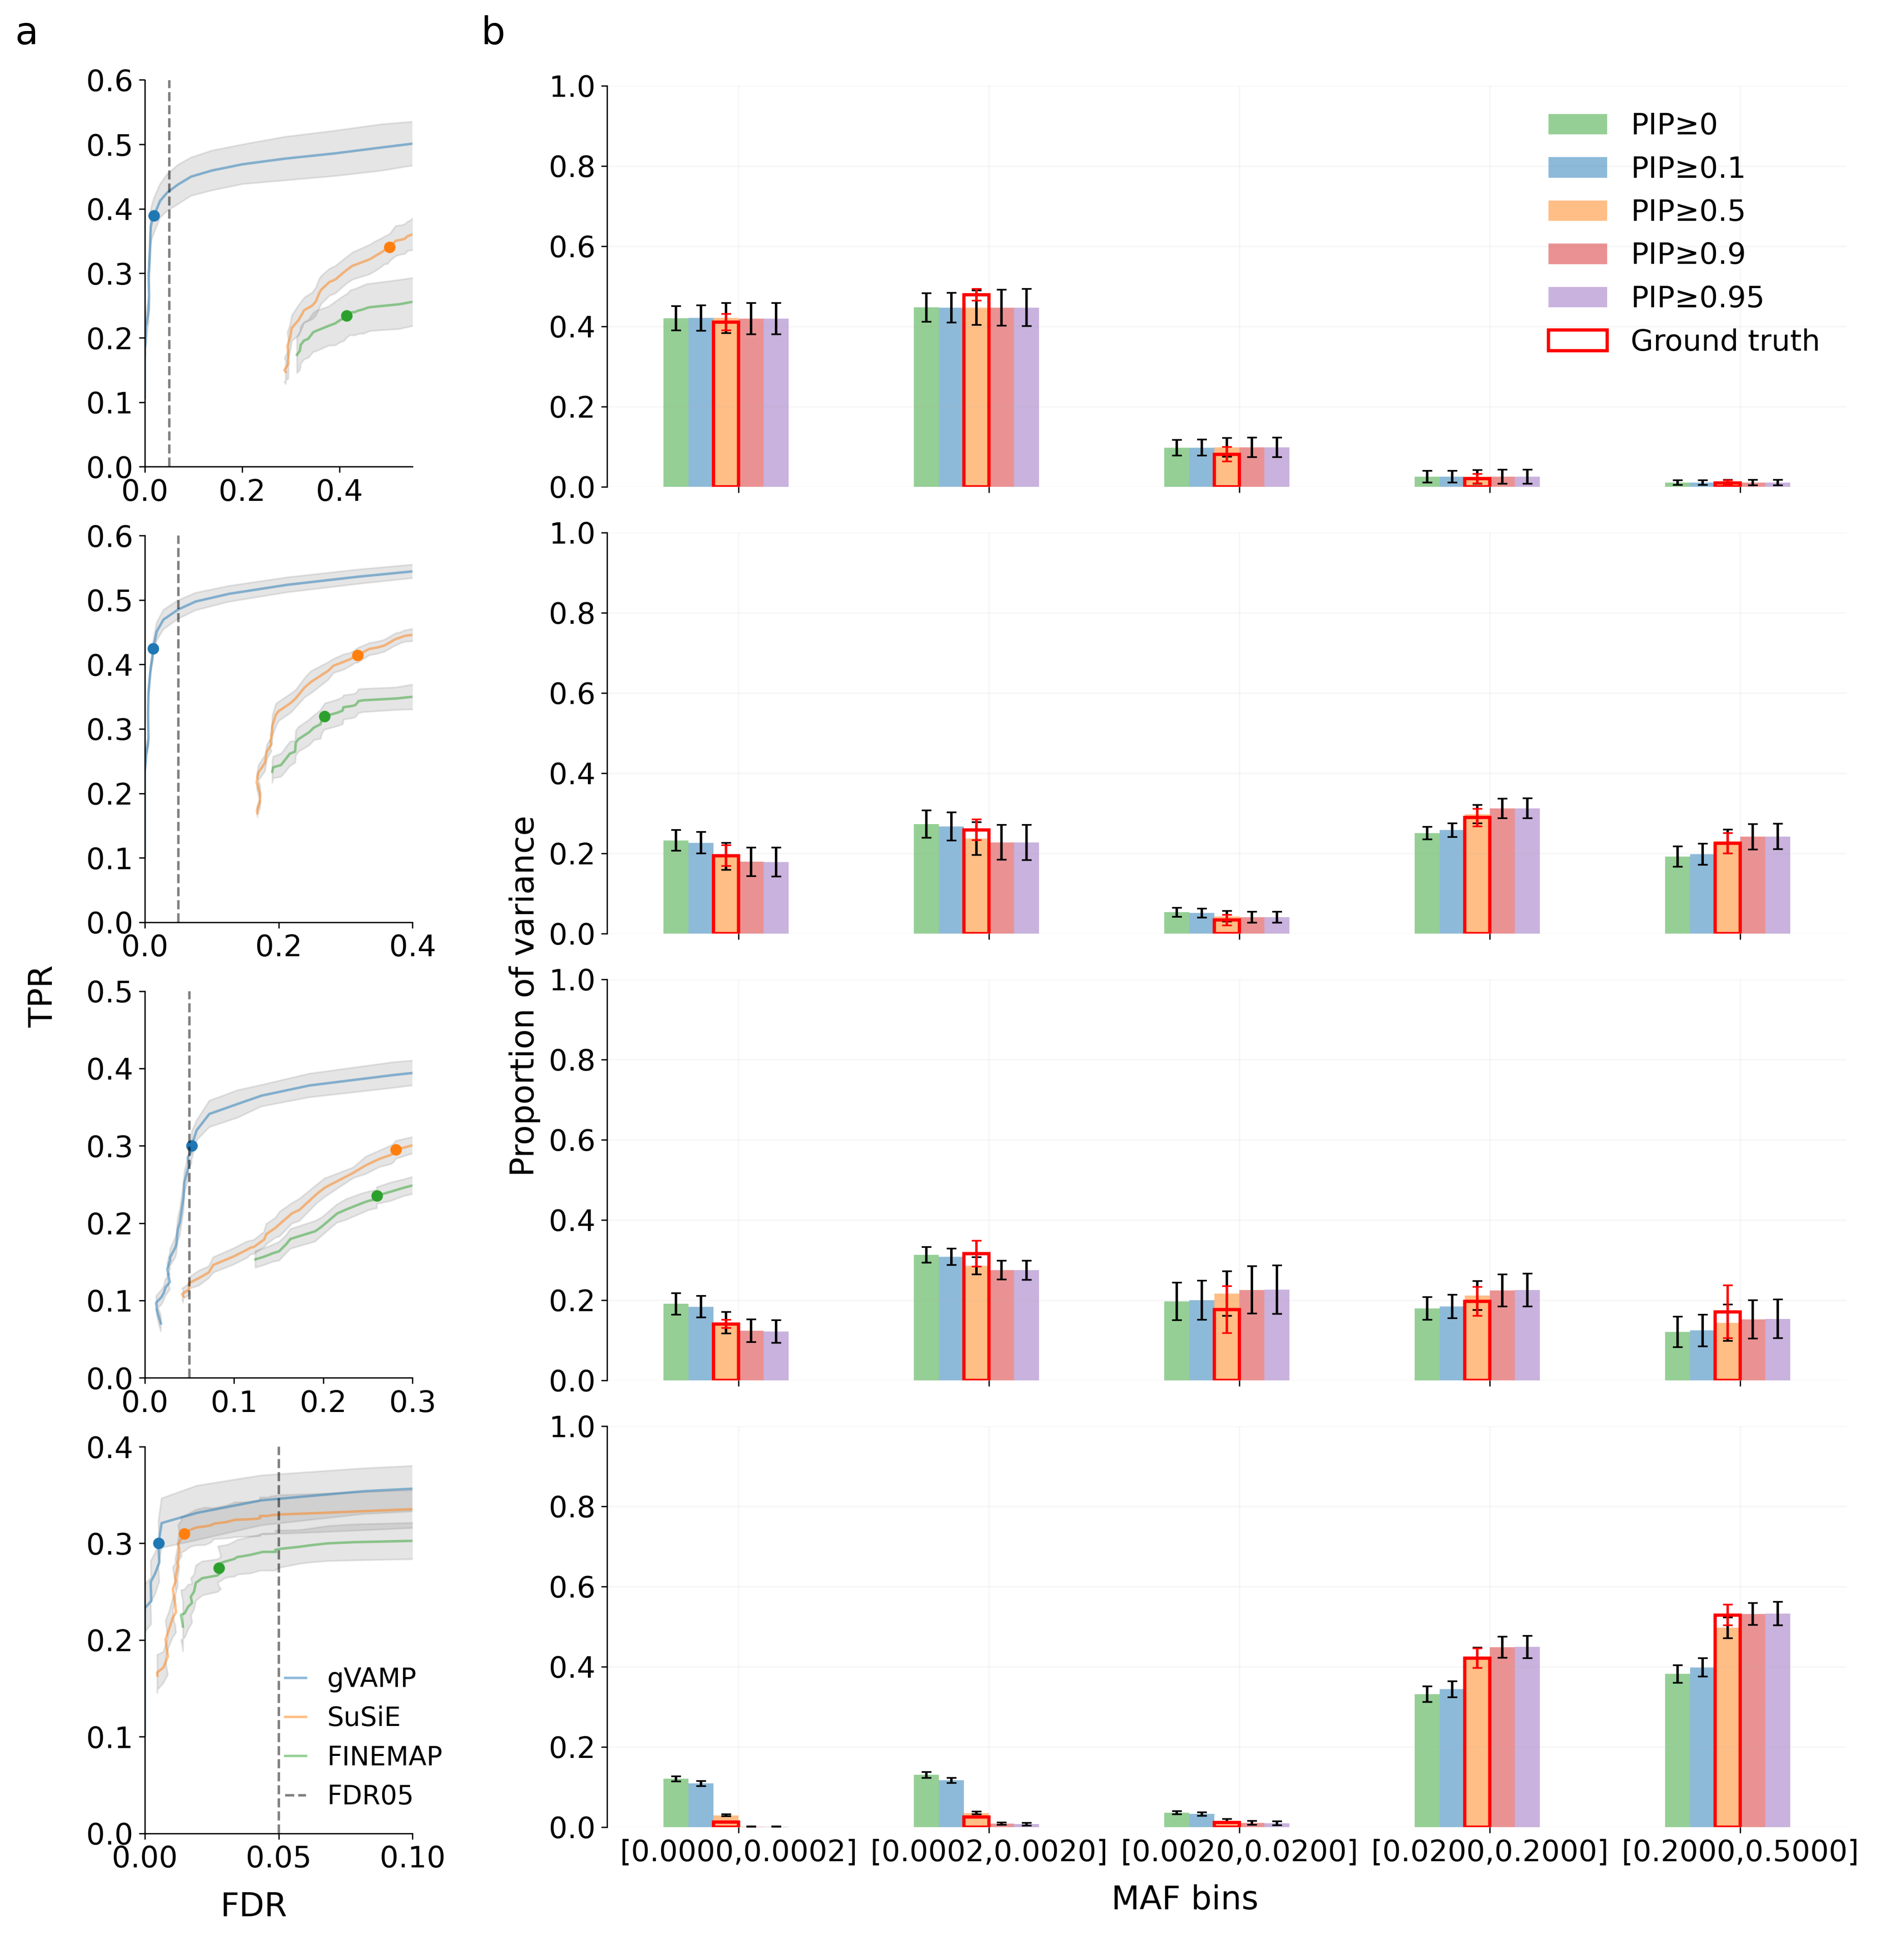
\includegraphics[width=\linewidth]{graphics/gVAMP_figures/v4/Fig1.png}
    \caption[Simulation study of variable selection performance using whole genome sequence (WGS) data of chromosomes 11 to 15 in the UK Biobank]{\textbf{Simulation study of variable selection performance using whole genome sequence (WGS) data of chromosomes 11 to 15 in the UK Biobank}. \small{(a) Comparison of the true positive rate (TPR, $y$-axis) versus the false discovery rate (\gls{fdr}, $x$-axis) between gVAMP (blue) and marginal GWAS association testing plus fine-mapping implemented in the FINEMAP (green) and SuSiE (orange) algorithms across four simulation scenarios. The rows of both (a) and (b) correspond to settings $a$, $b$, $e$, and $f$, which are described in the Methods, Supplementary Table \ref{table:S1} and Figures \ref{fig:finalFigS1} to \ref{fig:finalFigS3}, alongside additional simulation settings. For gVAMP, variable selection is conducted from posterior inclusion probability (PIP) values obtained from a single model run genome-wide. For FINEMAP and SuSiE, we use a Bonferroni corrected p-value significance threshold for marginal GWAS testing and then, having identified associated regions, we use the algorithms to obtain the PIP values to conduct variable selection.}}
    \label{fig:fig1}
\end{figure}

\begin{figure}[!t] % the continued legend, at the top of the page after the figure
    \ContinuedFloat
    \captionsetup{labelformat=continued}
    \caption[]{\small{Error bands give the standard deviation across 5 simulation replicates. The blue, green and orange dots give the TPR and FDR at PIP $\geq 0.95$ threshold, which should correspond to an FDR of $\leq 0.05$ if the model correctly conducts variable selection based on PIP values. (b) The proportion of variance attributable to DNA loci of different frequency. We plot the proportion of the sum of the squared regression coefficients attributable to variants of different frequency as estimated from gVAMP across different posterior inclusion probability (PIP) thresholds. The ground truth (red frame) is calculated as the sum of squared true effects across different frequency groups. The variance attributable to SNPs of different frequency matches the ground truth when selecting variants at posterior inclusion probability $\geq 0.5$. Error bars give the standard deviation across simulation replicates.}}
\end{figure}

\subsection{Variable selection in whole genome sequencing data}
We begin by modeling the UK Biobank WGS data, curating a set of 16,854,878 WGS variants observed for 426,462 individuals of European genetic ancestry. To create this set, we remove individuals of first-degree ancestry to avoid close-familial environmental sharing, and because of cloud computing restrictions, we group highly correlated common variants with absolute correlation $\geq0.6$, keeping all rare variation within the data with minor allele frequency, MAF, $\geq 0.0001$ (see Methods).

We first assess the ability of gVAMP to estimate genetic effects within this curated UK Biobank WGS dataset, by simulating 12 different scenarios on top of data from chromosomes 11-15 (3,285,117 SNPs). The 12 scenarios differ in: \emph{(i)} the relationship of effect size and MAF; \emph{(ii)} the ratio of common to rare causal variants; and \emph{(iii)} the number of causal variants (500 or 1000) that contribute $7.25\% $ to the phenotypic variance (see Methods and Supplementary Table \ref{table:S1} for an overview of the scenarios). Chromosomes 11-15 represent $\sim 18.8\%$ of the total length of the DNA and if we extrapolate genome-wide, then our simulated phenotypes would have $\sim 39\%$ phenotypic variance attributable to between approximately 2,700 and 5,300 underlying causal variants genome-wide. This gives an expected average variance contributed per DNA variant of $39\% / 5300 = 0.0074\%$, comparable to that of human height of $70\% / 10000 = 0.007\%$ suggested by recent results \cite{HTbig}. These settings are chosen to give adequate power to select variables and to enable clear comparisons of fine-mapping methods. We note also that in Supplementary Section \ref{supp:note1} we conduct extensive benchmarks of gVAMP in imputed SNP data for traits of highly polygenic architecture with different effect size distributions, different relationships of marker frequency and effect size, different numbers of causal variants and different variances attributable to the SNPs, across 12 additional settings each with 4 sets of data, for a total of hundreds of models trained with sample size $\sim 400$k and up to $>8$M SNPs (see Methods and Supplementary Section \ref{supp:note1}).

We analyze the WGS data with either: \emph{(i)} our proposed gVAMP; or \emph{(ii)} the FINEMAP \cite{10.1093/bioinformatics/btw018} and SuSiE variable selection models \cite{susie}, run on 3Mb regions surrounding each significant variant discovered via GWAS marginal testing one-SNP-at-a-time, following standard practice. With access to 2240 virtual CPU and just under 9TB (35 parallel instances of 256GB and 64 CPU), running gVAMP for all replicates of the 12 scenarios requires 5 days, with FINEMAP requiring 8 days. However, running SuSiE required 30 days to complete 4 scenarios (with standard LD and eigen-value calculation in LDstore2, see Methods), and given the consistently comparable performance to FINEMAP, we restrict our comparisons with SuSiE to only the settings presented in Figure \ref{fig:fig1}. 
We first calculate the true positive rate (TPR = number of identified variants that are causal / number of causal variants) and the false discovery rate (FDR = number of identified variants that are not causal / number of identified variants) at a given threshold. gVAMP shows improved power (TPR) for identifying the correct underlying causal variants and a well controlled FDR (FDR $\leq 5\%$ corresponding to a selection of variants with posterior inclusion probability, PIP, $\ge 95\%$), as compared to both the methods of FINEMAP and SuSiE across most scenarios (Figure \ref{fig:fig1}a and \ref{fig:finalFigS1} to \ref{fig:finalFigS3}). FINEMAP shows a well-controlled FDR in only five of the 12 settings (settings $f$, $h$, $j$, $k$ and $l$, in Figures \ref{fig:finalFigS1} to \ref{fig:finalFigS3}), where half of the simulated causal variants are common and the power relationship of minor allele frequency and effect size is weaker. In contrast, we find only two settings where the FDR of gVAMP rises slightly above $5\%$ (settings $i$ and $k$ in Figures \ref{fig:finalFigS1} to \ref{fig:finalFigS3}). In these two settings, the relationship between effect size and minor allele frequency is weakly negative and variants are distributed randomly across the WGS data. As a result, most causal variants are rare and each makes a very small contribution to the phenotypic variance, making them difficult to detect. Consequently, these are the lowest powered settings, where the TPR of both gVAMP and FINEMAP are the smallest and the fewest variants overall are recovered (Figure \ref{fig:finalFigS1}). gVAMP outperforms FINEMAP in terms of TPR in all but one scenario, namely the challenging setting $k$, where the TPR of both methods is low (Figures \ref{fig:finalFigS1} and \ref{fig:finalFigS3}). SuSiE performs similarly to FINEMAP as it is typically unable to control the FDR (Figure \ref{fig:fig1}a). SuSiE has higher TPR than FINEMAP, but it is still consistently outperformed by gVAMP, setting $f$ being the only one where all methods perform similarly (Figure \ref{fig:fig1}a).

The advantage of the gVAMP framework is confirmed in additional simulation comparisons. In particular, we find that infinitesimal versions of SuSiE and FINEMAP \cite{infinitesimalFineMapping2024} that have been proposed in the literature also show only slight improvements on the standard versions in all WGS settings we explored (Figure \ref{fig:finalFigS7}). Additionally, we find that variants selected by gVAMP at posterior inclusion probability $\geq 0.5$, have a frequency distribution that reflects the simulated ground truth across scenarios (Figure \ref{fig:fig1}b and \ref{fig:finalFigS4}). Furthermore, we validate the part of our analysis which combines WGS variants and WES burden scores by performing an additional set of simulations on top of WGS variants from chromosomes 11 to 15 and WES burden scores corresponding to that region of the DNA. We simulated signals with a total heritability of $h^2 = 7.25\%$ by allocating 75\% of $500$ causal markers to WGS variants and 25\% to WES burden scores, with WES burden scores exhibiting effect sizes with variance three-fold larger than those of individual WGS variants. This means that both groups should explain half the variance in settings where the variance of effect sizes is independent of the minor allele frequency. We find that we can correctly recover the percentage of variance recovered by each of the groups (Figure \ref{fig:S6}). Finally, when we simulate causal effects in both coding and non-coding regions, with 0\%, 50\%, or 100\% of the causal variants located in coding (exonic) regions, we find that as the percentage of causal variants allocated to coding regions increases so does the enrichment of the effects (Figure \ref{fig:S7new}). Taken all together, these findings suggest that existing methods fall short of the performance required for variable selection in WGS data, while gVAMP both reliably localizes the signal to the correct genomic regions and it selects a variant of appropriate frequency.

\subsection{The genetic architecture of human height in WGS data}
We then apply gVAMP to model the genetic architecture of human height in our 16,854,878 WGS variant dataset. We find significant amounts of common genetic variation detected and a considerable contribution of rare genetic variants (Figure \ref{fig:fig3}). Generally, the regions identified are replicated in the most recent GWAS study of human height~\cite{HTbig} within 100-500kb (Figure \ref{fig:fig3}a). We find that for variants of frequency $<0.05$ identified in the WGS analysis, variants discovered by Yengo \textit{et al.}~\cite{HTbig} of strongest correlation and most similar MAF, significant at $p\le5 \cdot 10^{-8}$ within a 500kb region, are more common in frequency (Figure \ref{fig:fig3}b).  Variants of frequency $<0.005$ discovered by gVAMP are likely not captured at all by Yengo \textit{et al.} because these variants have lower average marginal Chi-squared test statistic values than the other variants we identify (Figure \ref{fig:fig3}c) and Yengo \textit{et al.} set a MAF threshold of $1\%$ for their meta-analysis. We estimate the maximum correlation within the UK Biobank WGS data of each gVAMP discovery with Yengo \emph{et al.} SNPs significant at $p\le5 \cdot 10^{-8}$ within a 1 Mb window. We find that none of the variants of frequency $<0.005$ identified by gVAMP have a strong correlation with those identified by Yengo \textit{et al.} (Figure \ref{fig:correlation_MAF}). Thus, very rare gVAMP-identified variants are likely independent of the colocalizing common variants from Yengo \textit{et al.}, being simply a randomly selected set with higher frequency (Figure \ref{fig:fig3}b). In contrast, all gVAMP identified variants of frequency $\geq0.05$ are highly correlated to variants identified by Yengo \textit{et al.} (Figure \ref{fig:correlation_MAF}) with similar frequencies (Figure \ref{fig:fig3}b). Thus, consistent with the literature\cite{Wray.pbio}, common variant-tagged rare variant associations likely make up a small fraction of common-variant associations in Yengo \emph{et al.}, and taken together, our results suggest that discovered WGS regions are broadly the same as those previously identified.

\begin{figure}[p] % The legend continues in a second float on the next page.
    \centering   
    % 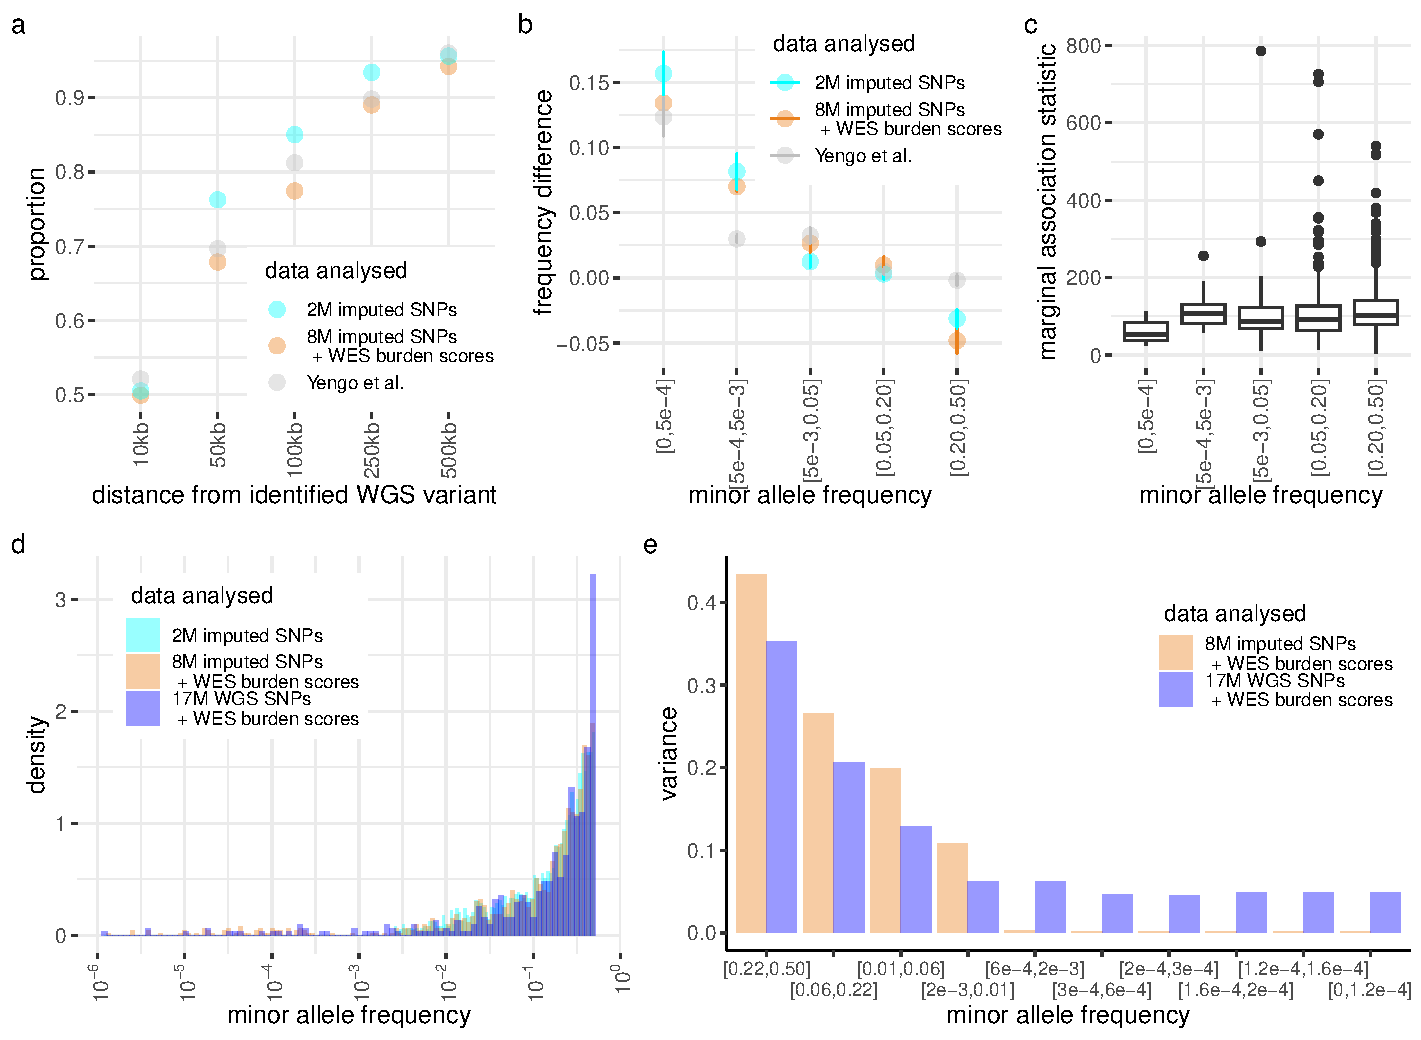
\includegraphics[width=16cm]{graphics/gVAMP_figures/final_main_Figure2.pdf}
    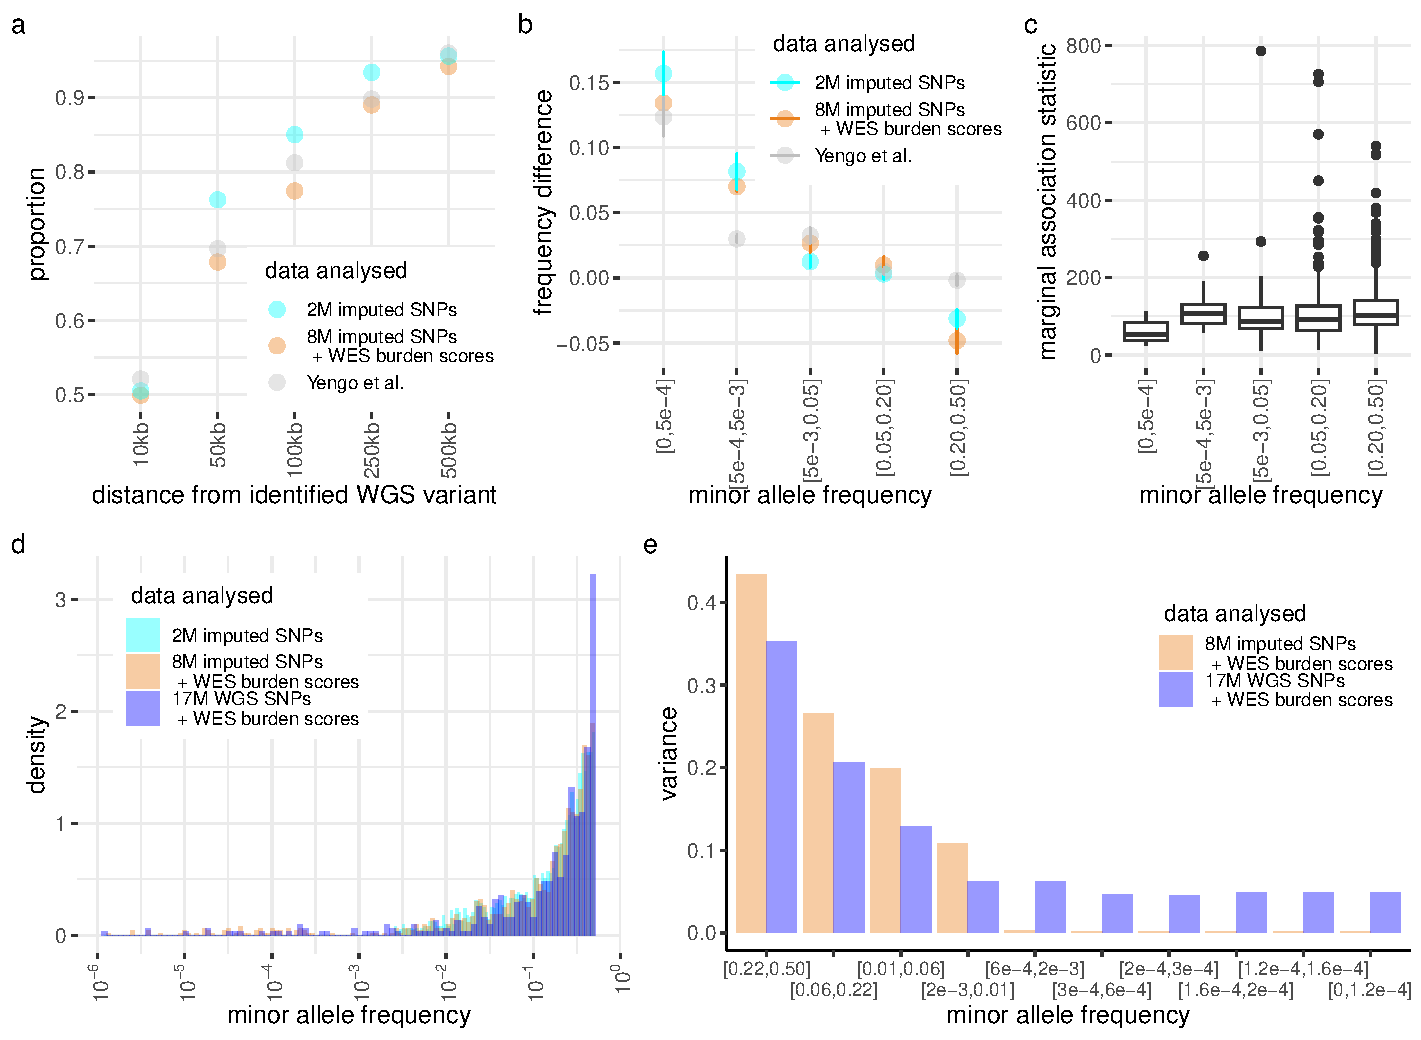
\includegraphics[width=0.95\textwidth]{graphics/gVAMP_figures/final_main_Figure2.pdf}
    \caption[The genetic architecture of human height inferred by gVAMP from 16,854,878 whole genome sequence variants in the UK Biobank]{\textbf{The genetic architecture of human height inferred by gVAMP from 16,854,878 whole genome sequence variants in the UK Biobank.} \small{\emph{(a)} For each whole genome sequence (WGS) variant discovered at  $\text{PIP}\ge 95\%$, we determine whether we also identify a variant within a given number of base pairs (distance, $x$-axis) from: \emph{(i)} the latest height GWAS study by Yengo \textit{et al.}~\cite{HTbig}, selecting variants at significance $p\le5 \cdot 10^{-8}$ from the marginal summary statistics for European individuals excluding the UK Biobank; or \emph{(ii)} an analysis of imputed SNP data with gVAMP, selecting variants with $\text{PIP}\ge 95\%$. The proportion overlap ($y$-axis) is calculated as the proportion of the identified WGS variants that are discovered within a certain base pair distance. \emph{(b)} For each WGS variant discovered at $\text{PIP}\ge 95\%$, we determine: \emph{(i)} the variant discovered by Yengo \textit{et al.} of most similar MAF significant at $p\le5 \cdot 10^{-8}$ within a 500kb region; or \emph{(ii)} the imputed variant of most similar minor allele frequency (MAF) discovered at $\text{PIP}\ge 95\%$ within a 500kb region. We then calculate the mean difference in MAF of the imputed/GWAS variant and the corresponding WGS variant, with error bars showing twice the standard error. \emph{(c)} For each WGS variant discovered at $\text{PIP}\ge 95\%$, we determine the maximum marginal association test statistic of any variant with absolute correlation $\ge0.6$. Boxplots of these maximum Chi-squared test statistic values are then given for different MAF groups, showing a drop in average power to detect rare variants. \emph{(Legend continued on the next page.)}}}
    \label{fig:fig3}
\end{figure}

\begin{figure}[!t] % the continued legend, at the top of the page after the figure
    \ContinuedFloat
    \captionsetup{labelformat=continued}
    \caption[]{\small{\emph{(d)} Density plot of the MAF distribution of all discovered variants at $\text{PIP}\ge 95\%$ for 2,174,071 imputed SNPs ("2M imputed SNPs"), 8,430,446 imputed SNPs fit jointly alongside 17,852 whole exome sequencing (WES) gene burden scores ("8M imputed SNPs + WES burden scores"), and 16,854,878 WGS SNPs fit jointly alongside 17,852 WES gene burden scores ("17M imputed SNPs + WES burden scores"). Irrespective of the data analyzed, the frequency distributions are similar, with the exception that the WGS analysis identifies a greater number of variants (both SNPs and gene burden scores) at lower frequencies. \emph{(e)} We calculate the proportional contribution to phenotypic variance across different MAF groups for 8,430,446 imputed SNPs fit jointly alongside 17,852 whole exome sequencing (WES) gene burden scores ("8M imputed SNPs + WES burden scores"), and 16,854,878 WGS SNPs fit jointly alongside 17,852 WES gene burden scores ("17M imputed SNPs + WES burden scores"). A larger proportion of variance is attributable to rare variation at the expense of more common variants in WGS data.}}
\end{figure}

\begin{figure}[p] % The legend continues in a second float on the next page.
    \centering
    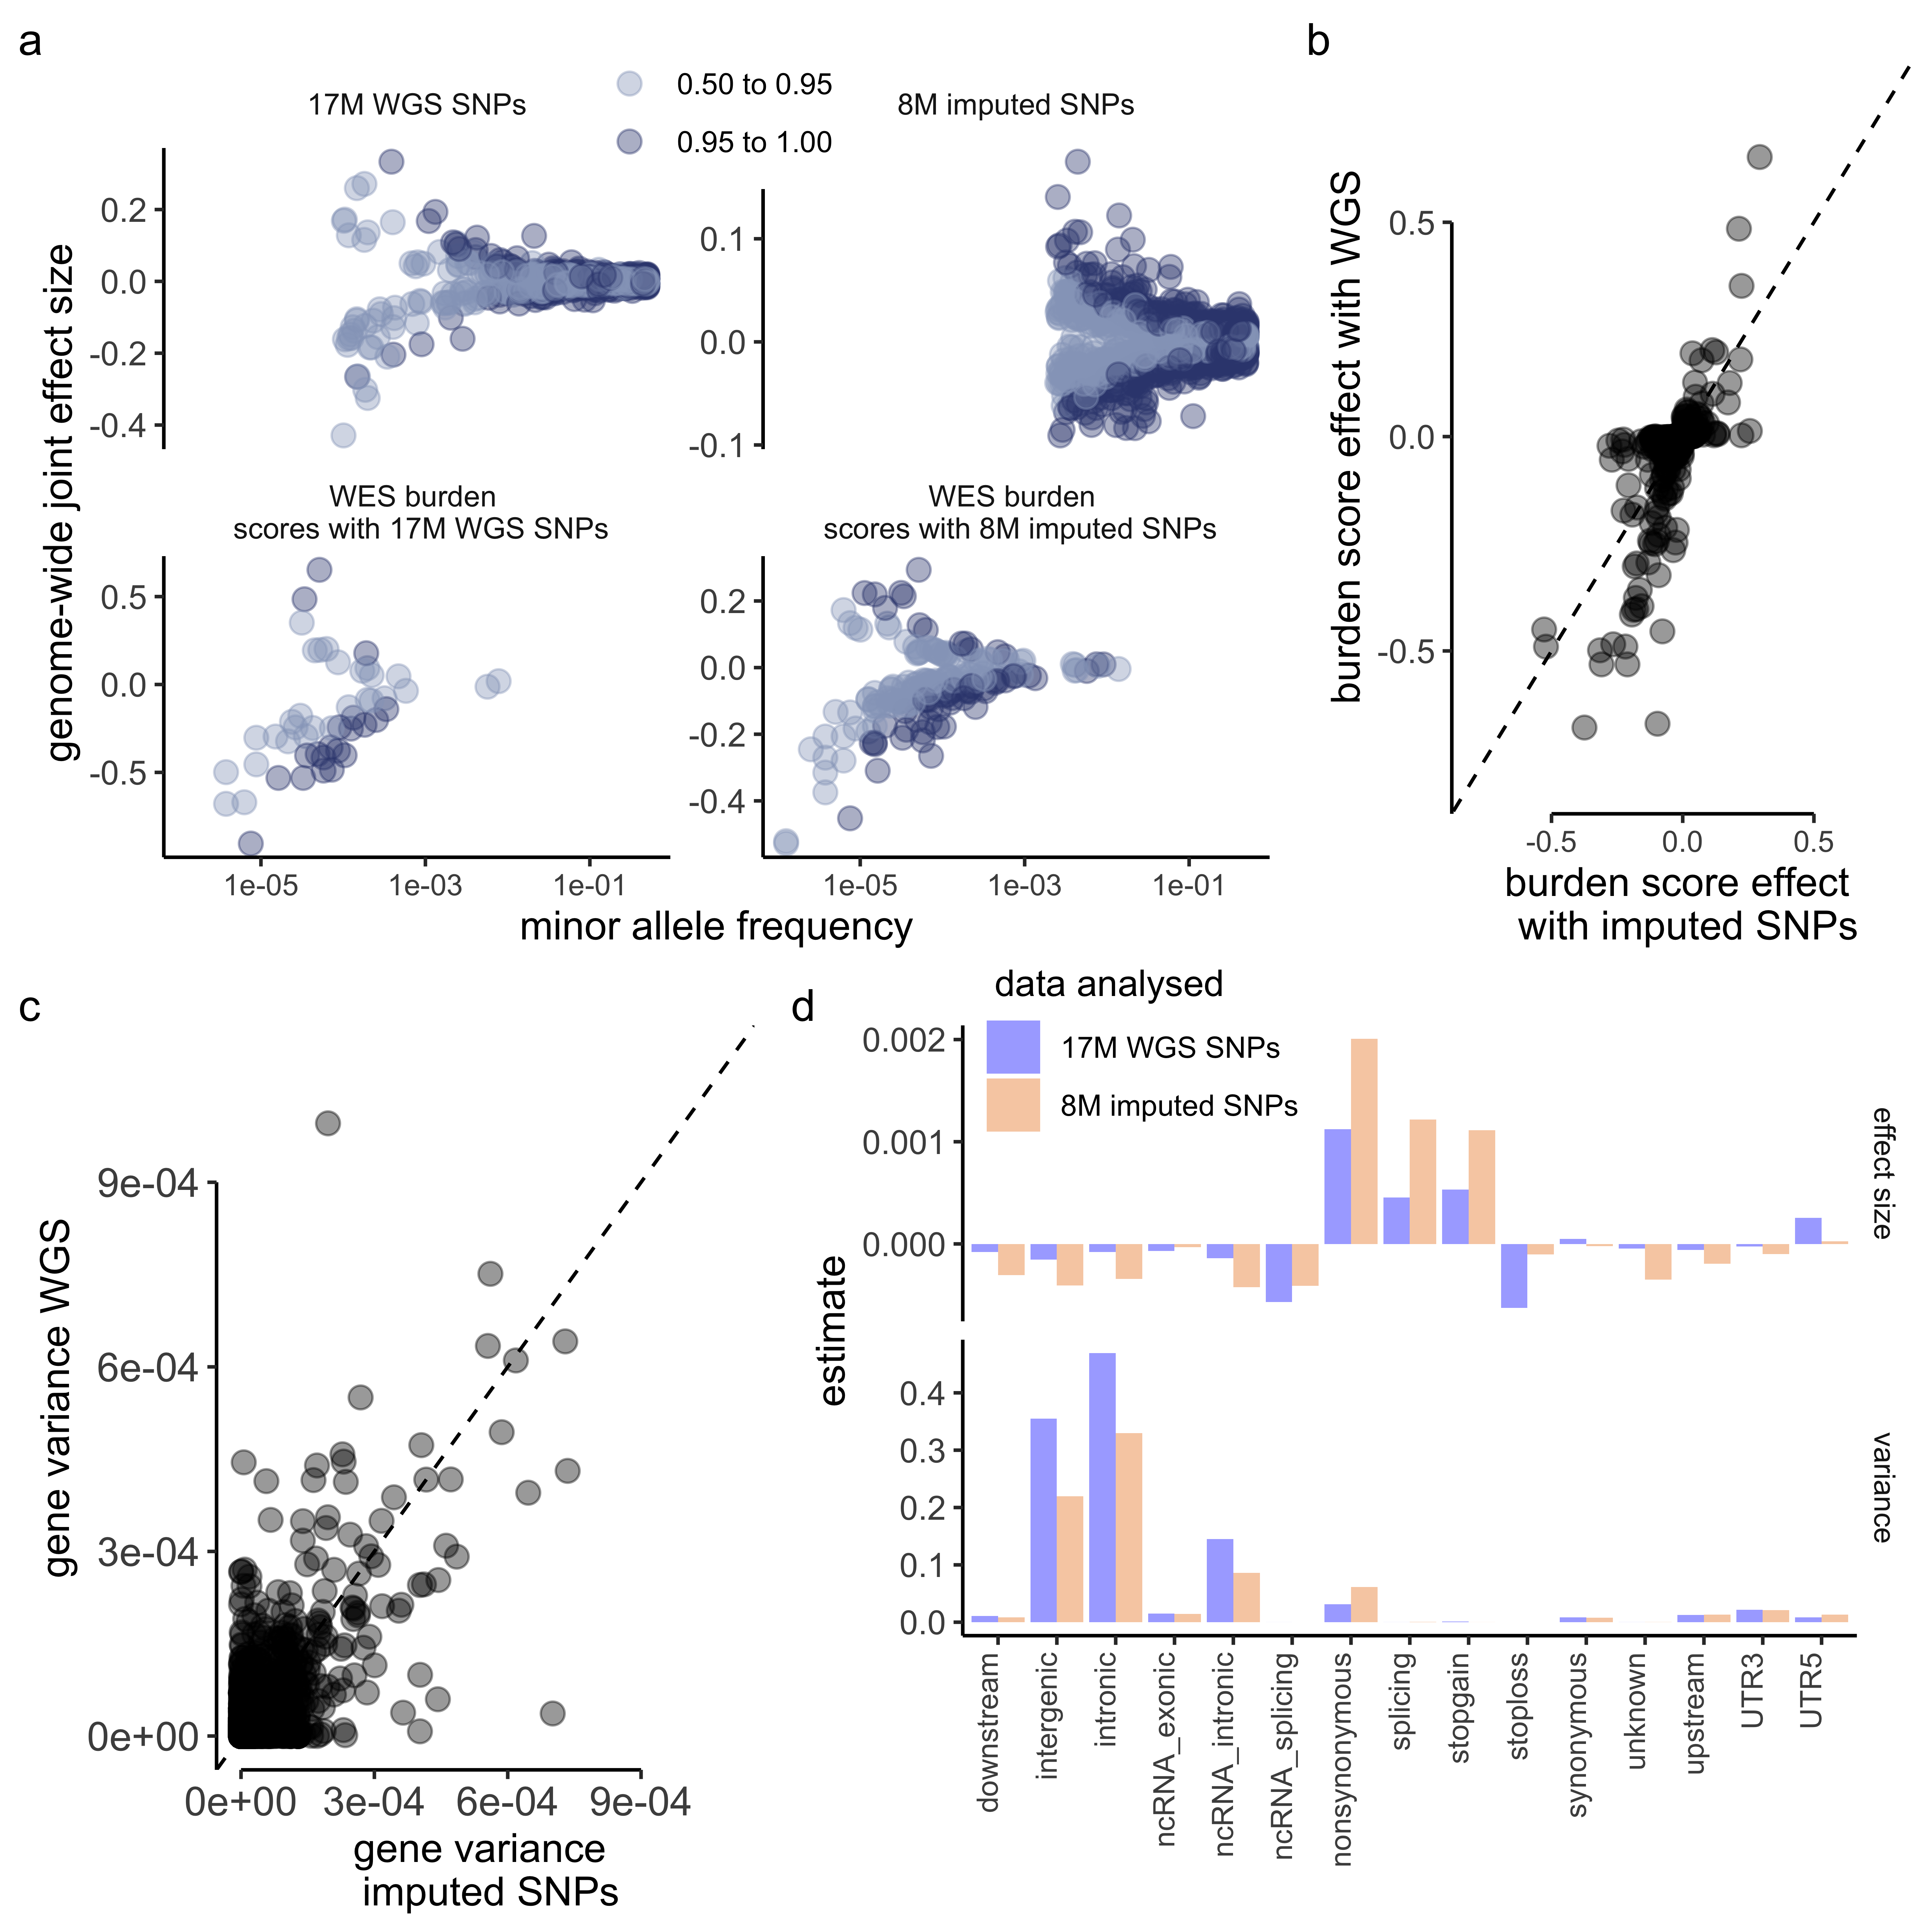
\includegraphics[width=\linewidth]{graphics/gVAMP_figures/final_main_figure_3.png}
    \caption[The relationship between effect size and minor allele frequency, burden score effects and the genetic architecture of human height inferred from 16,854,878 whole genome sequence variants in the UK Biobank]{\textbf{The relationship between effect size and minor allele frequency, burden score effects and the genetic architecture of human height inferred from 16,854,878 whole genome sequence (WGS) variants in the UK Biobank.} \small{\emph{(a)} For different posterior inclusion probability thresholds ($0.5$ to $0.95$ and $\ge0.95$), we plot the relationship between joint effect size and minor allele frequency (MAF) for 16,854,878 WGS variants ("17M WGS SNPs"), 8,430,446 imputed SNP variants ("8M imputed SNPs") and 17,852 whole exome sequence (WES) gene burden scores fit alongside either the WGS or imputed variants. \emph{(b)} Across 17,852 WES gene burden scores, we find general concordance of the estimated effect sizes when fit alongside either imputed or WGS data, for most but not all genes, with squared correlation 0.532 and regression slope 0.993 (0.007 SE). The dashed line gives $y=x$.}}
    \label{fig:fig4}
\end{figure}

\begin{figure}[!t] % the continued legend, at the top of the page after the figure
    \ContinuedFloat
    \captionsetup{labelformat=continued}
    \caption[]{\small{\emph{(c)} Likewise, we also find general concordance of the phenotypic variance attributable to markers annotated to each of the 17,852 genes, when fit conditional on either imputed or WGS variants, with squared correlation 0.494 and a regression slope of 0.698 (0.004 SE). The dashed line gives $y=x$. \emph{(d)} Finally, we show similar patterns of enrichment when annotating markers to functional annotations in either the average effect size relative to the genome-wide average effect size (labeled ``effect size'') or the proportion of variance attributable to each group (labeled ``variance''), from joint estimation of either imputed or WGS data.}}
\end{figure}

19 out of the 21 genome-wide significant gene burden scores are for genes that have previous GWAS height associations linked to them in Open Targets, but our analysis suggests that the effect is attributable to a rare protein coding variant rather than the common variants suggested by current genome-wide association studies. This includes insulin-like growth factor 2 genes IGF1R and IGF2BP2, and known height genes ACAN, ADAMTS10 and ADAMTS17, CRISPLD1, DDR2, FLNB, HMG20B, LTBP2, LCORL, NF1, and NPR2. Novel genes are COL27A1 which encodes a collagen type XXVII alpha 1 chain, and HECTD1. The top genes, where gVAMP attributes $\geq 0.04\%$ of height variation in addition to those listed above are EFEMP1, ZBTB38, and ZFAT. We find that many genome-wide significant height-associated rare variants discovered in the WGS data were not found in previous UK Biobank analyses in Open Targets including: rs116467226, an intronic variant by TPRG1; rs766919361, an intronic variant by FGF18; rs141168133, an intergenic variant 19kb from ID4; rs150556786, an upstream gene variant for GRM4; rs574843917, a non-coding transcript exon variant in GPR21; rs532230290, an intergenic variant 42kb from SCYL1; rs543038394, intronic in OVOL1; rs1247942912, a non-coding transcript exon variant in AC024257.3; rs577630729, a regulatory region variant for ISG20; and rs140846043, a non-coding transcript exon variant of MIRLET7BHG. 10 out of our top 38 height-associated WGS variants of $\leq1\%$ MAF were not previously discovered, and only become height-associated when conditioning on the entire polygenic background captured by WGS data within our analysis. 

Generally, marginal estimates made in WGS data for height have similar joint effect sizes when included within the gVAMP model (Figure \ref{fig:figS8}). We find high replication for variants directly observed within the All of Us study (Figure \ref{fig:figS9}) when we compare the jointly fitted gVAMP estimates to simple marginal OLS estimates made within All of Us, controlling for sex and 16 available PCs in (Figure \ref{fig:figS9}). The slope of the regression coefficients is $0.8471$, which is a previously used metric of replication \cite{yengo_meta-analysis_2018}.

We then compare our gVAMP WGS analysis to gVAMP run on two curated sets of 8,430,446 and 2,174,071 imputed SNPs for the same individuals (see Methods) but with an elevated MAF threshold, to contrast the findings obtained when setting different MAF thresholds, and to explore the benefit of using WGS data over imputed SNP data. gVAMP estimates the proportion of phenotypic variance in human height attributable to WGS data as 0.652, a value that is comparable to 0.63 for imputed SNP data, to the previously published REML estimate in a different WGS dataset~\cite{Wainschtein} and to family-based estimates~\cite{robinson2017}. This is expected as the imputed data are a subset of the WGS data and very low frequency variants are expected to make little contribution to the population-level variance, so that the addition of large numbers of rare variants will have little impact, especially if they capture signal that was previously weakly tagged by more common variation. 

gVAMP identifies 2,070 sets of variants when we apply the model to a set of 2,174,071 imputed SNPs at $\text{PIP}\ge 95\%$, which is consistent with findings from mixed-linear model association testing described in the next section within imputed data (Table \ref{table:table2}). We note that in the WGS data however, gVAMP identifies fewer genome-wide significant effects, with only 501 found at $\text{PIP}\ge 95\%$. There are two potential explanations for this. The first is that some of the height associations are re-allocated to DNA variants of lower minor allele frequency, and we then have lower power to detect them above a $\text{PIP}\ge 95\%$ threshold. The second explanation is that two variants can have very low correlation with each other in the imputed data, while still both being moderately correlated to a third SNP. If the third SNP is not in the imputed panel but is height associated, this would result in two quasi-independent associations in the imputed data, but only one in the WGS data. We find that our 501 findings are within 50kb of 1,042 of the 2,070 sets of variants identified by gVAMP in the 2,174,071 imputed SNP data and are within 500kb of 1,989 of the 2,070 variant sets. Thus, the WGS gVAMP findings are often neighbored by multiple variants discovered by gVAMP in the imputed SNP data. The WGS analysis identifies a greater proportion of variants (both SNPs and gene burden scores) at lower frequencies (Figure \ref{fig:fig3}d) and finds a larger proportion of variance attributable to rare variation at the expense of slightly less variation attributable to common variants (Figure \ref{fig:fig3}e). 

We show that rare effects are larger than the effects of common variants when both are fit jointly (Figure \ref{fig:fig4}a). We estimate the effects of 17,852 WES gene burden scores when fit alongside the WGS data, finding again that conditioning on rare variation enhances joint effect sizes (Figure \ref{fig:fig4}a and Figure \ref{fig:fig4}b). We find a general concordance of the estimated effect sizes for most but not all WES gene burden scores (Figure \ref{fig:fig4}b). WES gene burden score effects can differ in the WGS analysis by being either: \emph{(i)} more strongly associated because of improved conditioning on the genetic background, or \emph{(ii)} attenuated because the variants that comprise the burden score are also included as variants in the analysis. We sum up the joint effects to determine the variation in height attributable to each gene, and we find a general concordance across markers annotated to each of the 17,852 genes, conditional on all other markers, across the imputed SNP and WGS analysis (Figure \ref{fig:fig4}c). We see little relationship between the variance attributable to the burden score of a given gene and the SNPs annotated to the gene (Figure \ref{fig:figS10}), with some notable exceptions of: ACAN, ADAMTS17, ADAMTS10, and LCORL.
Additionally, across annotations, we find that the phenotypic variance attributable to different DNA regions is higher for intergenic and intronic variants (Figure \ref{fig:fig4}d). However, when adjusting for the number of SNPs contained by each category by using the average effect size of the group relative to the average effect size genome-wide, we find that exonic variants that are nonsynonymous, splicing and stop-gain have the largest average effects of the WGS variants included within our model (Figure \ref{fig:fig4}d). 
Finally, across annotations, we find similar patterns across both WGS and imputed SNP analyses (Figure \ref{fig:fig4}d). Taken together, we find strong concordance across WGS and imputed data analyses performed on the same people, but we highlight MAF cut-offs influence the variants to which effects are assigned and thus where phenotypic variance is allocated. Therefore, we expect WGS data to provide a more accurate characterization of the genetic architecture of human traits, but very large sample sizes are required to incorporate more rare variation so that effects can be appropriately assigned.

\subsection{Creating genetic predictors via gVAMP}

\begin{figure}[!t]
    \centering   
    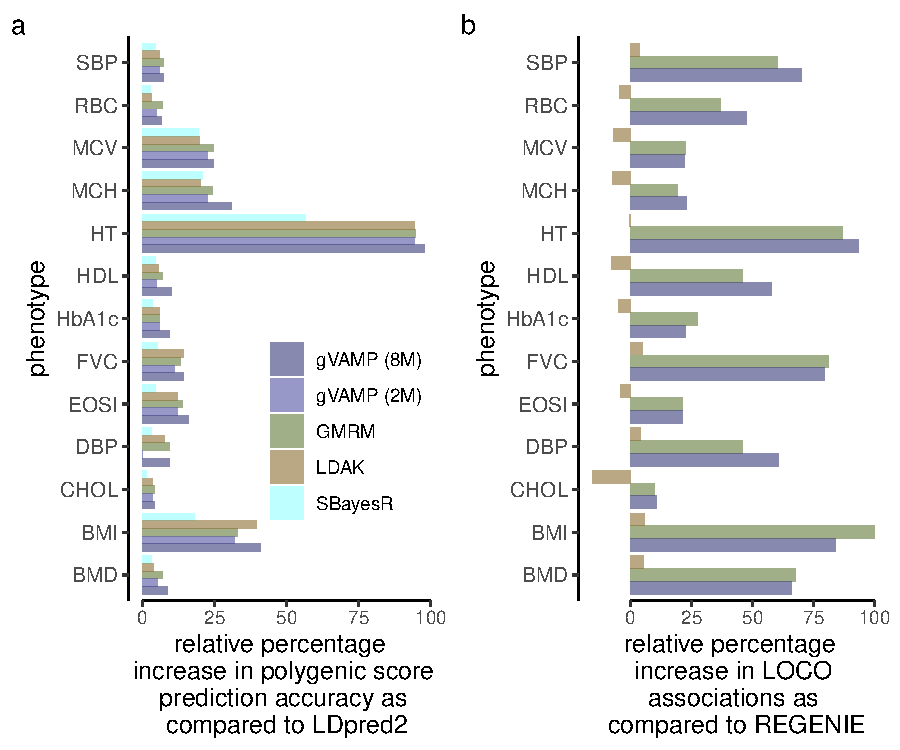
\includegraphics[width=1.0\linewidth]{graphics/gVAMP_figures/Figure_4.pdf}
    \caption[Validating gVAMP through polygenic risk score accuracy and association testing benchmarks in the UK Biobank within imputed SNP data]{\textbf{Validating gVAMP through polygenic risk score accuracy and association testing benchmarks in the UK Biobank within imputed SNP data.} \small{\emph{(a)} Relative prediction accuracy of gVAMP in a hold-out set of the UK Biobank across 13 traits as compared to other approaches. \emph{(b)} Relative number of leave-one-chromosome-out (\gls{loco}) associations of gVAMP across 13 UK Biobank traits as compared to other approaches at 8,430,446 markers.}}
    \label{fig:fig5}
\end{figure}


\begin{table}[!ht]
\caption[Polygenic risk score prediction accuracy $R^2$ for $13$ different traits from statistical models trained in the UK Biobank data and tested in a UK Biobank hold-out set]{\textbf{Polygenic risk score prediction accuracy $R^2$ for $13$ different traits from statistical models trained in the UK Biobank data and tested in a UK Biobank hold-out set.} \small Training data sample size and trait codes are given in Table \ref{table:tableS2} for each trait. The sample size of the hold-out test set is $15,000$ for all phenotypes. LDpred2 and SBayesR give estimates obtained from the LDpred2 and SBayesR software respectively, using summary statistic data of 8,430,446 SNPs obtained from the REGENIE software. LDAK gives the estimates obtained by the LDAK software using the elastic net predictor and individual-level data of 2,174,071 SNP markers. GMRM denotes estimates obtained from a Bayesian mixture model at 2,174,071 SNP markers (``GMRM 2.17M''). gVAMP denotes estimates obtained from the adaptive EM Bayesian mixture model within a vector approximate message passing (VAMP) framework presented in this work, using either 887,060 (``gVAMP 880k''), 2,174,071 (``gVAMP 2.17M''), or 8,430,446 SNP markers (``gVAMP 8M''). }
\begin{center}
\resizebox{\columnwidth}{!}{
\begin{tabular}{|| c || c || c || c || c || c | c | c ||} 
 \hline
Phen & LDpred2 & SBayesR & LDAK & GMRM & gVAMP & gVAMP & gVAMP \\ [0.5ex] 
     &        &         & 2.17M & 2.17M & 880k & 2.17M & 8M \\
\hline\hline
CHOL & 0.147 & 0.149 & 0.152 & \textbf{0.153} & 0.140 & 0.152 & \textbf{0.153} \\
 \hline 
EOSI & 0.107 & 0.112 & 0.120 & 0.122 & 0.114 & 0.120 & \textbf{0.124}  \\
 \hline 
HbA1c & 0.087 & 0.090 & 0.092 & 0.092 & 0.085 & 0.092 & \textbf{0.095}  \\
 \hline
HDL & 0.199 & 0.208 & 0.210 & 0.213 & 0.192 & 0.209 & \textbf{0.219} \\
 \hline
MCH & 0.178 & 0.215 & 0.214 & 0.221 & 0.203 & 0.218 & \textbf{0.223} \\
 \hline
MCV & 0.196 & 0.234 & 0.235 & \textbf{0.244} &  0.222 & 0.240 & \textbf{0.244} \\
 \hline
RBC & 0.186 & 0.191 & 0.192 & \textbf{0.199} & 0.182 & 0.195 & \emph{0.198} \\
 \hline
BMI & 0.100 & 0.118 & 0.140 & 0.133 & 0.107 & 0.132 & \textbf{0.141} \\
 \hline
DBP & 0.065 & 0.067 & 0.070 & \textbf{0.071} & 0.058 & 0.065 & \textbf{0.071} \\
 \hline
FVC & 0.098 & 0.103 & \textbf{0.112} & 0.111 & 0.097 & 0.109 & \textbf{0.112} \\
 \hline 
BMD & 0.188 & 0.194 & 0.195 & 0.201 & 0.183 & 0.198 & \textbf{0.204} \\
 \hline
HT & 0.231 & 0.362 & 0.449 & 0.450 & 0.419 & 0.449 & \textbf{0.457} \\
 \hline
SBP & 0.068 & 0.071 & 0.072 & \textbf{0.073} & 0.061 & 0.072 & \textbf{0.073} \\
\hline\hline
\end{tabular}
}
\end{center}
\label{table:table1}
\end{table}

We validate and benchmark gVAMP against state-of-the-art polygenic risk score prediction approaches in a number of alternative datasets. Applying our model to 13 traits in the UK Biobank imputed data (training data sample size and trait codes given in Table \ref{table:tableS2}), we compare the prediction accuracy of gVAMP to the widely used summary statistic methods LDpred2~\cite{ldpred} and SBayesR~\cite{sbayesr}, and to the individual-level methods GMRM~\cite{Orliac2022} and LDAK\cite{hof2024ldak}. gVAMP matches or outperforms all methods for most phenotypes (Figure \ref{fig:fig5}a and Table \ref{table:table1} with the best prediction accuracy highlighted in bold). Specifically, for human height (HT), our prediction accuracy is the highest and individual-level approaches clearly outperform summary statistic ones: we obtain an accuracy of 45.7\%, which is a 97.8\% relative increase over LDpred2 and a 26.2\% relative increase over SBayesR (Figure \ref{fig:fig5}a and Table \ref{table:table1}). We also note that our polygenic risk score has higher accuracy than that obtained from SBayesR using the latest height GWAS study of 3.5M people of 44.7\%~\cite{HTbig}, despite our sample size of only 414,055.

The polygenic risk score accuracy presented may represent the limit of what is achievable for these traits at the UK Biobank sample size. While modeling 2.17M SNPs improves accuracy over modeling 880,000 variants, we find rather small differences when going from 2.17M to 8M. This is because the 2.17M data set is an LD-grouped subset of the 8M data, and the addition of highly correlated variants captures little additional phenotypic variance. gVAMP estimates the $h^{2}_{SNP}$ of each of the 13 traits at an average of 3.4\% less than GMRM when using 2,174,071 SNP markers, but at an average of only 3.9\% greater than GMRM when using 8,430,446 SNP markers. This implies that only slightly more of the phenotypic variance is captured by the SNPs when the full imputed SNP data are used (Figure \ref{fig:figS12}). 

In summary, gVAMP (an adaptive mixture) performs similarly to LDAK (an elastic net) and GMRM (an MCMC sampling algorithm), improving over both when analyzing the full set of 8,430,446 imputed SNPs (Table \ref{table:table1} and Figure~\ref{fig:fig5}a).  

Next, we compare gVAMP to REGENIE, GMRM and LDAK-KVIK for association testing of the 13 traits in the UK Biobank imputed data. gVAMP performs similarly to mixed-linear model association leave-one-chromosome-out (MLMA-LOCO) testing conducted using a predictor from GMRM, with the use of the full 8,430,446 imputed SNP markers improving performance (Table \ref{table:table2} and Figure \ref{fig:fig5}b). REGENIE yields far fewer associations than either GMRM or gVAMP for all traits (Table \ref{table:table2} and Figure \ref{fig:fig5}b), with LDAK-KVIK being equivalent to REGENIE. We additionally verify that placing the predictors obtained by gVAMP into the second step of the LDAK-KVIK algorithm, also yields improved performance as compared to the LDAK model (Table \ref{table:tableS3}). Finally, using gVAMP to conduct variable selection, we find that hundreds of the LOCO marker associations for each trait can be localized (Table \ref{table:table2}), with the obvious caveat that these results are for imputed SNP data and re-analysis of WGS data may yield different results as we show above for height. Using height as an example, we find that 3,367 of the 5,242 MLMA-LOCO associations can be localized directly to the 2,070 imputed variant sets discovered by gVAMP via the PIP testing within 50kb. Thus, the gVAMP findings obtained by performing variable selection via the state evolution framework are often neighbored by multiple variants discovered by MLMA-LOCO in the imputed SNP data.

The increase in MLMA-LOCO findings for gVAMP over LDAK and REGENIE within the UK Biobank is consistent with the extensive simulation study results presented in Supplementary Section \ref{supp:note1}. There, we show that MLMA-LOCO testing power scales with the out-of-sample prediction accuracy only for gVAMP and not for the other methods (Figures \ref{fig:figSN1} and \ref{fig:figSN2}). Including more predictors in gVAMP to generate the polygenic risk scores used in the first stage of MLMA-LOCO generally improves out-of-sample prediction accuracy (Figure \ref{fig:figSN1}) and association testing power, whilst maintaining controlled type-I error (Figures \ref{fig:figSN2}, \ref{fig:figSN3}, \ref{fig:figSN4}). Additional simulations varying the number of markers included in the model lead to similar findings (Figures \ref{fig:figSN5}, \ref{fig:figSN6}, and \ref{fig:figSN7}). We also find that in practice our framework has similar performance to an MCMC approach, GMRM\cite{Orliac2022}, that has a similar mixture prior (Figure \ref{fig:figSN8}). 

In terms of compute time and resource use, gVAMP completes in less than $1/2$ of the time given the same data and compute resources as compared to a single trait analysis with REGENIE (Figure \ref{fig:figSN9}a), it is dramatically faster than GMRM ($12.5\times$ speed-up, Figure \ref{fig:figSN8}c), and it is marginally faster than LDAK when run on our simulated data (Figure \ref{fig:figSN9}a). Across the 13 UK Biobank traits, gVAMP is faster than LDAK-KVIK, but it requires more RAM (roughly the plink file size on disk, Figure \ref{fig:figSN9}b). If run on cloud computing at the current DNAnexus rates, step 1 of REGENIE can accommodate all 13 UK Biobank traits together, requiring 75.6 hours with 30 threads, 15GB RAM and 421GB disk space, which costs 75 GBP for the whole analysis, or 5.77 GBP per trait. LDAK-KVIK analysis of 13 UK Biobank traits with 2.17M SNPs using 15 threads, requires up to 6 GB of RAM and 210 GB of storage, with an average runtime across the 13 traits of 26h, giving an average cost of 11.47 GBP per trait. Increasing the CPU given to LDAK to 60 as in Figure \ref{fig:figSN9}b reduces the average run time to 14.5h, but raises costs to 28.57 GBP per trait. GMRM analysis of 2.17M SNP markers requires 82 hours using 60 threads and 210GB RAM and disk space, which costs 163.59 GBP per trait. In comparison, gVAMP analysis of 2.17M SNP markers requires 16 hours on average with 32 threads and 210GB RAM and disk space, which costs 20.59 GBP per trait. Increasing the CPU to 60 as in Figure \ref{fig:figSN9}b reduces the average run time to 11h, but slightly raises the cost to 21.89 GBP per trait.

\begin{table}[!ht]
\caption[Genome-wide significant associations for $13$ UK Biobank traits from the software GMRM, gVAMP, LDAK-KVIK and REGENIE at 8,430,446 genetic variants from either mixed linear model association leave-one-chromosome-out (MLMA-LOCO) testing or gVAMP variable selection]{\textbf{Genome-wide significant associations for $13$ UK Biobank traits from the software GMRM, gVAMP, LDAK-KVIK and REGENIE at 8,430,446 genetic variants from either mixed linear model association leave-one-chromosome-out (MLMA-LOCO) testing or gVAMP variable selection.} \small  "REGENIE 880k LOCO" denotes results obtained from MLMA-LOCO testing using the REGENIE software, with 882,727 SNP markers used for step 1 and 8,430,446 markers used for the LOCO testing of step 2. "GMRM 2M LOCO" refers to MLMA-LOCO testing at 8,430,446 SNPs, using a Bayesian MCMC mixture model in step 1, with 2,174,071 SNP markers. "LDAK 2M LOCO" refers to MLMA-LOCO testing at 8,430,446 SNPs, using the LDAK-KVIK software in step 1, with 2,174,071 SNP markers. "gVAMP 2M LOCO" refers to MLMA-LOCO testing at 8,430,446 SNPs, using the framework presented here, where in step 1 2,174,071 markers are used and the second step is identical to that of REGENIE. We then extend that to using all 8,430,446 SNP markers (``gVAMP 8M LOCO'') in step 1. We also present gVAMP posterior inclusion probability (PIP) testing when applying a correlation threshold on the markers prior to analysis of 0.9 to the SNP markers (2,174,071 markers). For LOCO testing, the values give the number of genome-wide significant linkage disequilibrium independent associations selected based upon a standard $p$-value threshold of less than $5 \cdot 10^{-8}$ and $R^2$ between SNPs in a 1 Mb genomic segment of less than $1\%$. For the PIP testing, values give the number of genome-wide significant associations selected based upon a $\geq0.95$ threshold.}
\begin{center}
\resizebox{\columnwidth}{!}{%
\begin{tabular}{|| c || c || c || c || c | c || c ||} 
 \hline
Trait & REGENIE & GMRM & LDAK & gVAMP & gVAMP & gVAMP \\ [0.25ex]
 & 880k LOCO & 2M LOCO & 2M LOCO & 2M LOCO & 8M LOCO & PIP \\ [0.25ex]
 \hline\hline
CHOL & 571 & 627 & 482 & 603 & \textbf{632} & 381 \\
 \hline 
EOSI & 572 & \textbf{693} & 549 & 630 & \textbf{693} & 527 \\
 \hline 
HbA1c & 337 & \textbf{429} &  321 & 385 & \emph{413} & 227 \\
 \hline
HDL & 692 & 1009 & 639 & 812 & \textbf{1092} & 536 \\
 \hline
MCH & 746 & 889 & 690 & 810 & \textbf{916} & 691 \\
 \hline
MCV & 970 & \textbf{1190} & 903 & 1062 & \emph{1185} & 898 \\
 \hline
RBC & 897 & 1229 & 856 & 1079 & \textbf{1325} & 651 \\
 \hline
BMI & 688 & \textbf{1376} & 726 & 1175 & \emph{1266} & 261\\
 \hline
DBP & 291 & 425 & 303 & 419 & \textbf{468} & 315 \\
 \hline
FVC & 549 & \textbf{994} & 577 & 721 & \emph{986} & 318 \\
 \hline 
BMD & 522 & \textbf{874} & 549 & 668 & \emph{867} & 491 \\
 \hline
HT & 2712 & 5070 & 2703 & 4452 & \textbf{5242} & 2070 \\
 \hline
SBP & 311 & 499 & 323 & 388 & \textbf{529} & 245 \\
\hline\hline
\end{tabular}
}
\end{center}
\label{table:table2}
\end{table}


\section{Discussion}
Here, we develop an adaptive form of Bayesian variable selection regression capable of fitting tens of millions of WGS variants jointly for hundreds of thousands of individuals. For human height, a joint analysis of a set of 17M WGS variants, localizes associations to numerous rare variants and gene burden scores as well as hundreds of regions containing common variation. gVAMP provides a point estimate from the posterior distribution and, as such, its performance is expected to match that of standard MCMC Gibbs sampling algorithms. We show that this is the case in imputed SNP data: gVAMP and GMRM have comparable out-of-sample prediction accuracy, comparable estimates of the proportion of variance attributable to the DNA, comparable number of MLMA-LOCO findings and comparable performance in our simulation study. However, unlike Gibbs sampling algorithms which cannot scale to current data sizes, gVAMP exhibits a remarkable speed-up which allows high-dimensional biobank data with full WGS observations to be analyzed. Taken together, gVAMP offers a flexible framework suitable to \emph{(i)} conduct variable selection in WGS data, where SuSiE, FINEMAP and their variants are miscalibrated, and \emph{(ii)} create polygenic risk scores with high accuracy that can also be used for downstream tasks such as MLMA-LOCO testing, with improved performance over LDAK-KVIK and REGENIE.

There are a number of remaining limitations and possible ways to expand and improve the analyses presented here. Our results suggest that the prioritization of relevant regions, genes and gene sets is feasible at current sample sizes, but the detection of specific height-associated mutations is expected to be a challenging task. There are a very large number of rare variants within the human population that are missing from our analysis of 16,854,878 WGS variants. While conducting variable selection genome-wide for these will require millions of WGS samples, it may be beneficial to include as many of these rare variants as possible. Our algorithm requires random-access memory (RAM) that is the same as the PLINK data file on disk, and although we evidence that this is not prohibitive to running the algorithm on the UK Biobank cloud computing, two alternative solutions could be to: \emph{(i)} apply gVAMP region-by-region, or \emph{(ii)} make slight modifications in the implementation, so that gVAMP streams data, at the cost of slightly increased run time. Our ongoing work focuses on exploring these options.

A further limitation is that we have exclusively tested and analyzed individuals of European ancestry. Combining data of different ancestries, or utilising admixed populations is of great importance~\cite{world}, and previous work suggests that better modeling within a single large biobank can facilitate improved association testing in other global biobanks~\cite{crosspred}. However, tackling this problem requires the development of a modeling framework that explicitly allows for differences in MAF, LD and effect size across the human population, which we leave to future work. 

Additionally, we also removed first-degree relatives from all of our analyses to avoid confounding of shared environmental effects. While some relatedness still exists even after removing first-degree relatives, we show in simulations that gVAMP performs well in both WGS and imputed data when planting a signal on real observed genotype data. Our motivation is that genotype-phenotype data of close relatives is often utilized for follow-up studies and there are unique models (to which our framework could be adapted) employed for such tasks. Additionally, removing first-degree relatives loses 39,592 individuals from the UK Biobank, which does not alter the sample size in a significant way. We note that methods such as fastGWA~\cite{fastGWAglm} or the equivalent implementation in LDAK, could be used where a first step calculates the parameters needed to control for environmental confounding before the model is then run. Furthermore, our method currently requires LD pruning of highly correlated common variants to improve numerical stability and convergence. While this limits the ability of gVAMP to fine-map regions with extremely high correlations, we note that when rare variants are included in the analysis, we find that gVAMP demonstrates superior performance compared to FINEMAP, SuSiE, and their respective variants.

Finally, we also now seek to extend the model presented here to different outcome distributions (binary outcomes, time-to-event, count data, etc.), to have a grouped prior for annotations, to model multiple outcomes jointly, and to do all of this using summary statistic as well as individual-level data across different biobanks. The latter objective is particularly feasible, as the VAMP iterations can be reformulated exclusively in terms of summary statistics. Progress in these areas has been made in the AMP literature, see e.g. \cite{schniter_vector_2016,Fletcher2019}. Combining data sets together in a principled way without a loss of accuracy, whilst preserving privacy, is key to obtaining the sample sizes that are likely required to fully explore the genetic basis of complex traits. We outline avenues for future research in Section \ref{sec:limitations_perspectives}.

% In this regard, we also seek to extend the inference framework to models that account for non-homogeneity of population, specifically setups in which the population is comprised of individuals of different genetic ancestry. To explore transfer learning abilities from overrepresented subpopulation to underrepresented subpopulations, several MCMC approaches that either directly model relationship between subpopulation effect sizes guided by global hyperparameters \cite{prscsx,mussel,JointPRS} or that use posterior mean of overrepresented population in prior construction for underrepresented subpopulations \cite{BridgePRS} have been developed. Upon estimation of effect sizes for all subpopulations, a typical approach is to fit a simple linear regression model between predictors obtained from each subpopulation and tune hyperparameters on the validation set of the targeted subpopulation. Hence, motivated by approach taken by \cite{BridgePRS} and work on AMP with side information \cite{AMP_side_info}, we propose conditioning on an additional state evolution result from overrepresented population when constructing denoisers for underrepresented population. Predictor obtained in such way would represent transfer learning component from one subpopulation to the other, implicitely searching for shared effect sizes, whilst performing training only on targeted supopulation. Such approach would enjoy benefits derived from using individual-level models over summary-level models, whilst being extremely computationally efficient as the overrepresented population effects sizes and state evolution parameters would need to be calculated only once and since training individual-level models in underrepresented subpopulations is much faster due to lower number of individuals involved. In terms of objects from Algorithm \ref{gVAMP}, instead of deriving $\mathbb{E}[\bm{\beta}|{\bm{r_{1,t}}^{(2)}} = \mathcal{N}(\bm{\beta}, (\gamma_{1,t}^{(2)})^{-1} \bm{I}), p(\bm{\beta})]$ for underrepresented population we propose deribving $\mathbb{E}[\bm{\beta} | \bm{r_{1,t}}^{(2)} = \mathcal{N}(\bm{\beta}, ({\gamma_{1,t}}^{(2)})^{-1} \bm{I}), {\bm{r_1}^{(1)}} = \mathcal{N}(\bm{\beta}, ({\gamma_{1}}^{(1)})^{-1} \bm{I}), p(\bm{\beta})]$, where objects $\bm{r_{1,t}}^{(2)} \text{ and } {\gamma_{1,t}}^{(2)}$ relate to underrepresented population and objects ${\bm{r_1}^{(1)}} \text{ and } {\gamma_{1}}^{(1)}$ represent state evolution parameters picked from the stopping iteration from the training of overrepresented subpopulation. The detailed derivation of these denoisers is provided in Supplementary Section \ref{supp:note3}.

% $\mathbb{E}[\bm{\beta} | \bm{r_{1,t}}^{(2)} = \mathcal{N}(\bm{\beta}, ({\gamma_{1,t}}^{(2)})^{-1} \bm{I}), {\bm{r}^{(1)}}_{1} = \mathcal{N}(\bm{\beta}, ({\gamma_{1}}^{(1)})^{-1} \bm{I}), p(\bm{\beta})]$, where objects $\bm{r_{1,t}}^{(2)} \text{ and } {\gamma_{1,t}}^{(2)}$ relate to underrepresented population and objects ${\bm{r}^{(1)}}_{1} \text{ and } {\gamma_{1}}^{(1)}$
% In this regard, we also seek to extend the model to allow for transfer learning across multi-ancestry datasets. One principled way of doing this similar to defining a prior on effect sizes for one ancestry based on the effect estimates from the other one \cite{BridgePRS}. One idea here would be to exploit on the uncertanty estimaton from state evolution results from primary population and use it as a side information inspired by the work on AMP with side information \cite{AMP_side_info}. Details of such derivation can be found in \ref{supp:note3}.

In summary, gVAMP is a different way to create genetic predictors and to conduct variable selection. With increasing sample sizes reducing standard errors, a vast number of genomic regions are being identified as significantly associated with trait outcomes by one-SNP-at-a-time association testing. Such large numbers of findings will make it increasingly difficult to determine the relative importance of a given mutation, especially in whole genome sequence data with dense, highly correlated variants. Thus, it is crucial to develop statistical approaches fitting all variants jointly and asking whether, given the LD structure of the data, there is evidence for an effect at each locus. 


\section{Methods}

\subsection{gVAMP algorithm}

\begin{breakablealgorithm}{genomic Vector Approximate Message Passing}{gVAMP}{gVAMP}
    \begin{algorithmic}[1]
        \STATE \parbox[t]{\dimexpr\linewidth-2\algorithmicindent}{% 
        {\bfseries Input:} preprocessed normalized genotype matrix $\bX \in \mathbb{R}^{N \times P}$, max number of iterations $N_{\text{it}}$, initial estimate of effect sizes $\bm{r}_{1,0} = \bm{0}_{P} \in \mathbb{R}^P$, initial estimate of effect sizes precision $\gamma_{1,0} = 10^{-6} > 0$, initial estimate of noise precision $\gamma_{\epsilon, 0}=2$, initial set of parameters defining the prior distribution $\Theta_{0} = \{\lambda, (\pi_{i}^{(0)})^{L}_{i=1}, \allowbreak (\sigma_{i}^{(0)})^{L}_{i=1} \}$, max number of variance auto-tuning steps $N_{\text{var\_tune}} = 5 \in \mathbb{N}$, threshold for stopping criterion $\varepsilon = 10^{-4} > 0$, damping factor $\rho \in (0, 1), \allowbreak \alpha_{2,-1} = 0.$}
        \FOR{$t = 0, 1,\dots, N_{\text{it}}$}
            \STATE {\bfseries Denoising step}

            \FOR{$k = 0, 1,\dots, N_{\text{var\_tune}}$ }
                \STATE $\hat{\bm{\beta}}_{1,t} = \mathbb{E}[\bm{\beta} | \bm{r}_{1,t} = \bm{\beta} + \mathcal{N}(0, \gamma_{1,t}^{-1}\bm{I}), \gamma_{1,t}, \Theta_{t}]$
                \IF {$t>0$}
                    \STATE Variance auto-tuning step of estimation error for $\bm\beta$ in the denoising step, called $\gamma_{1,t}$ 
                    \STATE \text{EM} update of the prior distribution parameters $\Theta$, called $\Theta_t$
                    \IF {$|\gamma_{1,t}-\gamma_{1,t}^{(\text{previous})}|< 10^{-3} $}
                        \STATE \textbf{break}
                    \ENDIF
                \ENDIF
            \ENDFOR
            \IF {$t\ge0$}
                \STATE $\hat{\bm{\beta}}_{1,t} = \rho \cdot \hat{\bm{\beta}}_{1,t} + (1-\rho) \cdot \hat{\bm{\beta}}_{1,t-1}$
            \ENDIF
            \STATE $\alpha_{1,t} = \gamma_{1,t} \cdot \langle \text{Var}[\bm{\beta}|\bm{r}_{1,t} = \bm{\beta} + \mathcal{N}(0, \gamma_{1,t}^{-1}\bm{I}), \gamma_{1,t}, \Theta_{t}] \rangle$
            \STATE $\gamma_{2,t} = \gamma_{1,t} \cdot (1 - \alpha_{1,t}) / \alpha_{1,t}$ 
            \STATE $\bm{r}_{2,t} = (\hat{\bm{\beta}}_{1,t} - \alpha_{1,t} \bm{r}_{1,t}) / (1-\alpha_{1,t})$
            \STATE $\xi = \min (2\cdot \min(\alpha_{1,t}, \alpha_{2,t-1}), 1.0)$ 
            % // Inspired by \cite{VAMP_MRI,sarkar2021mri}
            \STATE $\rho = \max(\rho, \xi)$
            \item[]
            \STATE \textbf{LMMSE step}
            \STATE $\hat{\bm{\beta}}_{2,t} =  ( \gamma_{\epsilon,t} \bm{X}^\top\bm{X} + \gamma_{2,t} \bm{I} )^{-1} ( \gamma_{\epsilon,t} \bm{X}^\top \bm{y} + \gamma_{2,t} \bm{r}_{2,t} )$ 
            \STATE $\alpha_{2,t} = \gamma_{2,t} \cdot \text{Tr}[(\gamma_{\epsilon,t} \bm{X}^\top\bm{X} + \gamma_{2,t}\bm{I})^{-1}] / P$
            \STATE $\gamma_{1,t+1} = \gamma_{2,t} \cdot (1-\alpha_{2,t}) / \alpha_{2,t}$
            \IF {$t>1$}
                % \STATE Variance auto-tuning step of estimation error for $\bm\beta$ in the LMMSE step, called $\gamma_{2,t}$
                \STATE \parbox[t]{\dimexpr\linewidth-3\algorithmicindent}{%
                    Variance auto-tuning step of estimation error for $\bm\beta$ in the LMMSE step, called $\gamma_{2,t}$}
            \ENDIF
            \STATE $\bm{r}_{1,t+1} = (\hat{\bm{\beta}}_{2,t} - \alpha_{2,t} \bm{r}_{2,t}) / (1-\alpha_{2,t})$ 
            \STATE { \text{EM update of the estimate of } $\gamma_{\epsilon}$\text{, called } $\gamma_{\epsilon,t}$ }
            \item[]
            \IF {$t\ge 1$ and $||\hat{\bm{\beta}}_{1,t} - \hat{\bm{\beta}}_{1,t-1}||_2 / ||\hat{\bm{\beta}}_{1,t-1}||_2 < \varepsilon$}
                \STATE \textbf{break}
            \ENDIF
        \ENDFOR
        \STATE \textbf{return} $\hat{\bm{\beta}}_{1,t}$
    \end{algorithmic}
\end{breakablealgorithm}

Approximate message passing (AMP) was originally proposed for linear regression \cite{DMM09, Bayati2011, krzakala2012} assuming a Gaussian design matrix $\bX$. To accommodate a wider class of structured design matrices, vector approximate message passing (\gls{vamp}) was introduced in \cite{schniter_vector_2016}. The performance of VAMP can be precisely characterized via a deterministic, low-dimensional \emph{state evolution} recursion, for any right-orthogonally invariant design matrix. We recall that a matrix is right-orthogonally invariant if its right singular vectors are distributed according to the Haar measure, i.e., they are uniform in the group of orthogonal matrices. Empirical evidence \cite{donoho2009observed, monajemi2013deterministic} suggests that the predictions for rotationally invariant models hold for a wide class of scenarios, and a line of work  has aimed at showing that this is case for AMP algorithms \cite{Wang22AMPUniversality, dudeja2022universality}.

gVAMP extends EM-VAMP, introduced in \cite{LearningFreeEnergies2018, RigorousDynamics2017}, in which the prior parameters are adaptively learnt from the data via EM, and it is an iterative procedure consisting of two steps: \emph{(i)} denoising, and \emph{(ii)} linear minimum mean squared error (LMMSE) estimation. The denoising step accounts for the prior structure given a noisy estimate of the signal $\bm{\beta}$, while the LMMSE step utilizes phenotype values to further refine the estimate by accounting for the LD structure of the data.

A key feature of AMP-type algorithms is the so-called Onsager correction: this is added to ensure the asymptotic normality of the noise corrupting the estimates of $\bm{\beta}$ at every iteration. Here, in contrast to MCMC or other iterative approaches, the normality is guaranteed under mild assumptions on the normalized genotype matrix. This property allows a precise performance analysis via state evolution and, consequently, the optimization of the method.

In particular, the quantity $\gamma_{1,t}$ in line 7 of Algorithm \ref{gVAMP} is the state evolution parameter tracking the error incurred by $\bm r_{1, t}$ in estimating $\bm\beta$ at iteration $t$. The state evolution result gives that $\bm{r}_{1,t}$ is asymptotically Gaussian, i.e., for sufficiently large $N$ and $P$, $\bm{r}_{1,t}$ is approximately distributed as $\mathcal{N}(\bm{\beta}, \gamma_{1,t}^{-1} \bm{I})$. Here, $\bm{\beta}$ represents the signal to be estimated, with the prior learned via EM steps at iteration $t$: 
% \begin{align}
%     \beta_i \sim (1-\lambda_t) \cdot \delta_0(\cdot) + \lambda_t \cdot \sum^{L}_{l=1} \pi_{t, l} \cdot \mathcal{N}(\cdot, 0, \sigma_{t, l}^2), \quad \,\forall \,\, i = 1, \dots, P.
% \end{align}
\begin{align}
    \beta_i \sim (1-\lambda_t) \cdot \delta_0 + \lambda_t \cdot \sum^{L}_{l=1} \pi_{t, l} \cdot \mathcal{N}(0, \sigma_{t, l}^2), \quad \,\forall \,\, i = 1, \dots, P.
\end{align}
Compared to Equation \eqref{eq:prior_gvamp}, the subscript $t$ in $\lambda_t, \pi_{t, l}, \sigma_{t, l}$ indicates that these parameters change through iterations, as they are adaptively learned by the algorithm.
Similarly, $\bm{r}_{2,t}$ is approximately distributed as $\mathcal{N}(\bm{\beta}, \gamma_{2,t}^{-1} \bm{I})$. The Gaussianity of $\bm{r}_{1,t}, \bm{r}_{2,t}$ is enforced by the presence of the Onsager coefficients $\alpha_{1,t}$ and $\alpha_{2,t}$, see lines 17 and 24 of Algorithm \ref{gVAMP}, respectively. We also note that  $\alpha_{1,t}$ (resp.\ $\alpha_{2,t}$) is the state evolution parameter linked to the error incurred by $\hat{\bm \beta}_{1, t}$ (resp.\ $\hat{\bm \beta}_{2, t}$).

The vectors $\bm r_{1, t}, \bm r_{2, t}$ are obtained after the LMMSE step, and they are further improved via the denoising step, which respectively gives $\hat{\bm \beta}_{1, t}, \hat{\bm \beta}_{2, t}$. In the denoising step, we exploit our estimate of the approximated posterior by computing the conditional expectation of $\bm\beta$ with respect to $\bm r_{1, t}, \bm r_{2, t}$ in order to minimize the mean square error of the estimated effects. For example, let us focus on the pair $(\bm r_{1, t}, \hat{\bm \beta}_{1, t})$  (analogous considerations hold for $(\bm r_{2, t}, \hat{\bm \beta}_{2, t})$). Then, we have that 
\begin{align}
    \label{denoiser_def}
\hat{\bm \beta}_{1, t} = f_t(\bm{r}_{1,t}) = \mathbb{E}[\bm{\beta} | \bm{r}_{1,t} = \bm{\beta} + \mathcal{N}(0, \gamma_{1,t}^{-1}\bm{I}), \lambda_t, \{\pi_{t, l}\}_{l=1}^L, \{ \sigma_{t,l}^2 \}_{l=1}^L].
\end{align}
Here, $f_t:\mathbb{R} \to \mathbb{R}$ denotes the denoiser at iteration $t$ and the notation $f_t(\bm{r}_{1,t})$ assumes that the denoiser $f_t$ is applied component-wise to elements of $\bm{r}_{1,t}$. Note that, in line 15 of Algorithm \ref{gVAMP}, an additional damping step is performed on the denoised signal estimate as suggested in \cite{rangan_vector_2019}, see ``Algorithm stability'' below. In line 20 of Algorithm \ref{gVAMP}, inspired by \cite{VAMP_MRI,sarkar2021mri}, we tune the damping factor to ensure that each iteration of the algorithm acts as a contraction mapping.
% Note that, in line 15 of Algorithm \ref{gVAMP}, we take this approach one step further by performing an additional step of damping, see ``Algorithm stability'' below. 

From Bayes' theorem, following the approach in \cite{EMGAMP2012}, one can calculate the posterior distribution (which here has the form of a spike-and-slab mixture of Gaussians) and obtain its expectation. Hence, by denoting a generic component of $\bm{r}_{1,t}$ as $r_1$, it follows that
\begin{align}
    \label{denoiser}
    & f_t(r_1) \nonumber \\
    & = \frac{\lambda_t \cdot \sum_{l=1}^L \pi_{t,l} \cdot \frac{r_1 \cdot \sigma_{t,l}^{2}}{\gamma_{1,t}^{-1} + \sigma_{t,l}^{2}} \cdot \mathcal{N}(r_1; 0, \gamma_{1,t}^{-1} + \sigma_{t,l}^{2})}{ (1-\lambda_t) \cdot \mathcal{N}(r_1; 0, \gamma_{1,t}^{-1}) + \lambda_t \sum_{l=1}^L \pi_{t,l} \cdot \mathcal{N}(r_1; 0, \gamma_{1,t}^{-1} + \sigma_{t,l}^2) } \nonumber \\
    & = \frac{\lambda_t \cdot \sum_{l=1}^L \pi_{t,l} \cdot \frac{r_1 \cdot \sigma_{t,l}^2}{(\gamma_{1,t}^{-1} + \sigma_{t,l}^{2})^{3/2}} \cdot \text{EXP}(\sigma_{t,l}^2) }{(1-\lambda_t) \cdot \gamma_1^{1/2} \cdot \text{EXP}(0) + \lambda_t \cdot \sum_{l=1}^L \pi_{t,l} \cdot \frac{1}{(\gamma_{1,t}^{-1} + \sigma_{t,l}^2)^{1/2}} \cdot \text{EXP}(\sigma_{t,l}^2)}, 
\end{align}
where $\mathcal{N}(r_1; 0, \gamma_{1,t}^{-1} + \sigma_{t,l}^{2})$ denotes the probability density function of a Gaussian with mean $0$ and variance $\gamma_{1,t}^{-1} + \sigma_{t,l}^{2}$ evaluated at $r_1$. Furthermore, we set 
\begin{align}
    \text{EXP}(\sigma^2) = \exp \bigg ( - \frac{r_1^2}{2} \cdot \frac{\sigma_{t,*}^2 - \sigma^2}{(\gamma_{1,t}^{-1} + \sigma^2) (\gamma_{1,t}^{-1} + \sigma_{t, *}^2)} \bigg ),
\end{align} 
with $\sigma_{t,*}^2:= \max_{l}(\sigma_{t,l}^2)$. This form of the denoiser is particularly convenient, as we typically deal with very sparse distributions when estimating genetic associations. We also note that the calculation of the Onsager coefficient in line 17 of Algorithm \ref{gVAMP} requires the evaluation of a conditional variance, which is computed as the ratio of the derivative of the denoiser over the error in the estimation of the signal, i.e., 
\begin{multline}
    \label{den_onsager}
    \operatorname{Var}\Big[\beta_i \,\Big|\, (\bm{r}_{1,t})_i = \beta_i + \mathcal{N}(0, \gamma_{1,t}^{-1}),\ \lambda_t,\ \{\pi_{t,l}\}_{l=1}^L,\ \{\sigma_{t,l}^2\}_{l=1}^L\Big] \\
    = \frac{f_t'\big((\bm{r}_{1,t})_i\big)}{\gamma_{1,t}}.
\end{multline} 
The calculation of the derivative of $f_t$ is detailed in Supplementary Section \ref{supp:note2}, following \cite{EMGAMP2012}.

If one has access to the singular value decomposition (SVD) of the data matrix $\bm{X}$, the per-iteration complexity is of order $\mathcal{O}(N P)$. However, at biobank scales, performing the SVD is computationally infeasible. Thus, the linear system $( \gamma_{\epsilon,t} \bm{X}^\top\bm{X} + \gamma_{2,t} \bm{I} )^{-1}(\gamma_{\epsilon, t} \bm{X}^\top \bm{y} + \gamma_{2,t} \bm{r}_{2,t})$ (see line $23$ of Algorithm \ref{gVAMP}) needs to be solved using an iterative method, in contrast to having an analytic solution in terms of the elements of the singular value decomposition of $\bm{X}$. In the next section, we provide details on how we overcome this issue.

\subsubsection{Scaling up using warm-start conjugate gradients}
Following \cite{schniter2021gampmatlab}, we approximate the solution of the linear system $( \gamma_{\epsilon,t} \bm{X}^\top\bm{X} + \gamma_{2,t} \bm{I} )^{-1}(\gamma_{\epsilon, t} \bm{X}^\top \bm{y} + \gamma_{2,t} \bm{r}_{2,t})$ with a symmetric and positive-definite matrix via the \textit{conjugate gradient method} (CG), see Algorithm \ref{CG} in Supplementary Section \ref{supp:note4}, which is included for completeness. If $\kappa$ is the condition number of $\gamma_{\epsilon,t} \bm{X}^\top\bm{X} + \gamma_{2,t} \bm{I}$, the method requires $\mathcal{O}(\sqrt{\kappa})$ iterations to return a reliable approximation. 

Additionally, inspired by \cite{schniter2021gampmatlab,skuratovs2022warmstarting}, we initialize the CG iteration with an estimate of the signal from the previous iteration of gVAMP. This warm-starting technique leads to a reduced number of CG steps that need to be performed and, therefore, to a computational speed-up. However, this comes at the expense of potentially introducing spurious correlations between the signal estimate and the Gaussian error from the state evolution. Such spurious correlations may lead to algorithm instability when run for a large number of iterations (also extensively discussed below). This effect is prevented by simply stopping the algorithm as soon as the $R^2$ measure on the training data starts decreasing.
% i.i.d.
In order to calculate the Onsager correction in the LMMSE step of gVAMP (see line $22$ of Algorithm \ref{gVAMP}), we follow standard practice \cite{schniter2021gampmatlab} and use the Hutchinson estimator \cite{Hutchinson} to estimate the quantity $\text{Tr}[(\gamma_{\epsilon,t} \bX^\top \bX + \gamma_{2,t} \bm{I})^{-1}]/P$. We recall that this estimator is unbiased, in the sense that, if $\bm{u}$ has \gls{iid} \ entries equal to $-1$ and $+1$ with the same probability, then
\begin{align}
    \mathbb{E}[\bm{u}^\top(\gamma_{\epsilon,t} \bX^\top \bX + \gamma_{2,t} \bm{I})^{-1}\bm{u}/ P ] = \text{Tr}[(\gamma_{\epsilon,t} \bX^\top \bX + \gamma_{2,t} \bm{I})^{-1}]/P.
\end{align}    
Furthermore, in order to perform an EM update for the noise precision $\gamma_\epsilon$, one has to calculate the trace of a matrix which is closely connected to the one we have seen in the previous paragraph. In order to do so efficiently, i.e., to avoid solving another large-dimensional linear system, we store the inverted vector $(\gamma_{\epsilon,t} \bX^\top \bX + \gamma_{2,t} \bm{I})^{-1}\bm{u}$ and reuse it again in the EM update step (see the subparagraph on EM updates).

\subsubsection{Algorithm stability}
We find that the application of existing EM-VAMP algorithms to the UK Biobank dataset leads to diverging estimates of the signal. This is due to the fact that the data matrix (the SNP data) might not conform to the properties required in \cite{rangan_vector_2019}, especially that of right-rotational invariance. Furthermore, incorrect estimation of the noise precision in line 30 of Algorithm \ref{gVAMP} may also lead to instability of the algorithm, as previous applications of EM-VAMP generally do not leave many hyperparameters to estimate.

To mitigate these issues, different approaches have been proposed including row or/and column normalization, damping (i.e., doing convex combinations of new and previous estimates) \cite{VAMP_MRI,sarkar2021mri}, and variance auto-tuning \cite{RigorousDynamics2017}. In particular, to prevent EM-VAMP from diverging and ensure it follows its state evolution, we empirically observe that the combination of the following techniques is crucial.  
\begin{enumerate}
    \item \emph{Damping} is performed in the space of denoised signals. Thus, line 15 of Algorithm \ref{gVAMP} reads as
    \begin{equation}
        \hat{\bm{\beta}}_{1,t} = \rho \cdot \mathbb{E}[\bm{\beta} | \bm{r}_{1,t}, \Theta_{t}] + (1-\rho) \cdot \hat{\bm{\beta}}_{1,t-1},
    \end{equation}   
in place of $\hat{\bm{\beta}}_{1,t} = \mathbb{E}[\bm{\beta} | \bm{r}_{1,t}, \Theta_{t}]$. Here, $\rho \in ( 0, 1 )$ denotes the damping factor. This ensures that the algorithm makes smaller steps when updating a signal estimate. 
    \item \emph{Auto-tuning} of $\gamma_{1,t}$ is performed via the approach from \cite{RigorousDynamics2017}. Namely, in the auto-tuning step, one refines the estimate of $\gamma_{1,t}$ and the prior distribution of the effect size vector $\bm{\beta}$ by jointly re-estimating them. Denoting the previous estimates of $\gamma_{1, t}$ and $\Theta$ with $\gamma_{1, t}^{(\text{previous})}$ and $\Theta^{(\text{previous})}$, then this is achieved by setting up an expectation-maximization procedure whose aim is to maximize 
\begin{align}
    \mathbb{E} \big [ \log p(\bm{\beta}, \bm{r}_{1, t}|\gamma_{1, t}, \Theta) | \bm{r}_{1, t}, \gamma_{1, t}^{(\text{previous})}, \Theta^{(\text{previous})} \big ]
\end{align}
with respect to $\gamma_{1, t}$ and $\Theta$.
\item 
The design matrix is \emph{filtered} for first-degree relatives to reduce the correlation between rows, which has the additional advantage of avoiding potential confounding of shared-environmental effects among relatives. 
\end{enumerate}

\subsubsection{Estimation of the prior and noise precision via EM}
The VAMP approach in \cite{rangan_vector_2019} assumes exact knowledge of the prior on the signal $\bm\beta$, which deviates from the setting in which genome-wide association studies are performed. Hence, the signal prior must be adaptively learned from the data using expectation-maximization (EM) steps, see lines 8 and 30 of Algorithm \ref{gVAMP}. This leverages the variational characterization of EM-VAMP \cite{LearningFreeEnergies2018}, and its rigorous theoretical analysis presented in \cite{RigorousDynamics2017}. In this subsection, the hyperparameter estimation results from \cite{EMGAMP2012} are summarized in the context of our model. The final update formulas for the hyperparameter estimates are as follows:
\begin{itemize}
    \item \underline{Sparsity rate $\lambda$:} 
The quantities $\{\zeta_j \}_{j=1}^P$ are defined as: $\forall j=1, \dots, P,$
% One-line denominator: the equation uses the full text width, not the narrower list width.
\begin{adjustwidth}{-\leftmargin}{0pt}
\begin{align}
    \label{em:mixture_probs}
    \zeta_j := \frac{\lambda_t \sum_{l=1}^L \pi_{l,t}\, \mathcal{N}\big((\bm{r}_{1,t})_j; 0, \sigma_{l,t}^2 + \gamma_{1,t}^{-1}\big)}{\lambda_t \sum_{l=1}^L \pi_{l,t}\, \mathcal{N}\big((\bm{r}_{1,t})_j; 0, \sigma_{l,t}^2 + \gamma_{1,t}^{-1}\big) + (1-\lambda_t)\, \mathcal{N}\big((\bm{r}_{1,t})_j; 0, \gamma_{1,t}^{-1}\big)}
\end{align}
\end{adjustwidth}
The intuition behind $\{\zeta_j\}_{j=1}^P$ is that each $\zeta_j$ tells what fraction of posterior probability mass was assigned to the event that it has a non-zero effect. Then, the update formula for the sparsity rate $\lambda_{t+1}$ reads as
\begin{align}
    \lambda_{t+1} = \frac{1}{P} \sum_{j=1}^P \zeta_j.
\end{align}
\item \underline{Probabilities of mixture components in the slab part $\{ \pi_{i} \} _{i=1}^L:$} Similarly, the quantities $\{\xi_{j,i}\}_{i=1, j=1}^{L,P}$ are defined as: $\forall i=1, \dots, L$, $\forall j=1,\dots, P$,
\begin{align}
    \xi_{j,i} := \frac{\pi_{i,t}\, \mathcal{N}\big((\bm{r}_{1,t})_j; 0, \sigma_i^2 + \gamma_{1,t}^{-1}\big)}{\sum_{l=1}^L \pi_{l,t}\, \mathcal{N}\big((\bm{r}_{1,t})_j; 0, \sigma_l^2 + \gamma_{1,t}^{-1}\big)}.
\end{align}
The intuition behind $\{\xi_{j,i}\}_{i=1, j=1}^{L,P}$ is that each $\xi_{j,i}$ approximates the posterior probability that a marker $j$ belongs to a mixture $i$ conditional on the fact that it has non-zero effect. Thus, the update formula for $\pi_{i,t+1}$ reads as: $\forall i=1,\dots, L$,
\begin{align}
    \pi_{i,t+1} = \frac{\sum_{j=1}^P \zeta_{j} \xi_{j,i}}{\sum_{j=1}^P \zeta_j}.
\end{align}

\item \underline{Variances of mixture components in the slab part $ \{ \sigma_{i}^2 \}_{i=1}^L:$} Using the same notation, the update formula reads as: $\forall i=1, \dots, L$,
\begin{align}
    \sigma_{i, t+1}^2 = \frac{\sum_{j=1}^P \zeta_j \cdot \xi_{j,i} \cdot \bigg [ \bigg ( \frac{(\bm{r}_{1,t})_j \cdot \gamma_{1,t}}{\gamma_{1,t} + \sigma_{i,t}^{-2}} \bigg )^2 + \frac{1}{\gamma_{1,t} + \sigma_{i,t}^{-2}} \bigg ] }{\sum_{j=1}^P \zeta_j \cdot \xi_{j,i}}.
\end{align}
Here we also introduce a mixture merging step, i.e., if the two mixtures are represented by variances that are close to each other in relative terms, then we merge those mixtures together. Thus, we adaptively learn the mixture number. 
\item $\underline{ \text{Precision of the error } \gamma_\epsilon }:$ Defining $\bm{\Sigma}_t := (\gamma_{\epsilon,t} \bm{X}^\top\bm{X} + \gamma_{2,t} \bm{I})^{-1}$ . Then, the update formula for the estimator of $\gamma_{\epsilon}$ reads as
\begin{align}
    \gamma_{\epsilon, t+1} = \frac{1}{\frac{||\bm{y} - \bm{X} \hat{\bm{\beta}}_{2,t}||^2}{N} + \frac{\text{Tr}(\bm{X} \bm{\Sigma}_t \bm{X}^\top)}{N}}.
\end{align}
In the formula above, the term $||\bm{y} - \bm{X} \hat{\bm{\beta}}_{2,t}||^2 / N$ takes into account the quality of the fit of the model, while the term $\text{Tr}(\bm{X} \bm{\Sigma}_t \bm{X}^\top) / N$ prevents overfitting by accounting for the structure of the prior distribution of the effect sizes via the regularization term $\gamma_{2,t}$. Note that the naive evaluation of this term would require an inversion of a matrix of size $P \times P$. We again use the Hutchinson estimator for the trace to approximate this object, i.e., $\text{Tr}(\bm{X} \bm{\Sigma}_t \bm{X}^\top) = \text{Tr}(\bm{X}^\top \bm{X} \bm{\Sigma}_t) \approx \bm{u}^\top (\bm{X}^\top \bm{X} \bm{\Sigma}_t) \bm{u}$, where $\bm{u}$ has i.i.d.\ entries equal to $-1$ and $+1$ with the same probability. Furthermore, instead of solving a linear system $\bm{\Sigma}_t \bm{u}$ with a newly generated $\bm{u}$, we re-use the $\bm{u}$ sampled when constructing the Onsager coefficient, thus saving the time needed to construct the object $\bm{\Sigma}_t \bm{u}$. 
\end{itemize}

\subsubsection{C++ code optimization}
Our open-source gVAMP software (\url{https://github.com/Information-and-learning-for-genomics/gVAMP}) is implemented in C++, and it incorporates parallelization using the OpenMP and MPI libraries. MPI parallelization is implemented in a way that the columns of the normalized genotype matrix are approximately equally split between the workers. OpenMP parallelization is done on top of that and used to further boost performance within each worker by simultaneously performing operations such as summations within matrix vector product calculations. Moreover, data streaming is employed using a lookup table, enabling byte-by-byte processing of the genotype matrix stored in PLINK format with entries encoded to a set $\{0,1,2\}$:

\begin{center}    
$
        \begin{pNiceMatrix}[margin]
        \Block[draw, fill=red!15,rounded-corners]{1-2}{}
        0 & 1 & 
        \Block[draw, fill=red!15,rounded-corners]{1-2}{}
        0 & 0 & 
        \Block[draw, fill=red!15,rounded-corners]{1-2}{}
        1 & 1 &
        \Block[draw, fill=red!15,rounded-corners]{1-2}{}
        1 & 0 \\
        \end{pNiceMatrix} \mapsto \begin{pNiceMatrix}[margin]
        \Block[draw, fill=darkgray!15,rounded-corners]{1-1}{}
        \text{NaN} & 
        \Block[draw, fill=darkgray!15,rounded-corners]{1-1}{}
        2 & 
        \Block[draw, fill=darkgray!15,rounded-corners]{1-1}{}
        0 &
        \Block[draw, fill=darkgray!15,rounded-corners]{1-1}{}
        1 \\
        \end{pNiceMatrix}
    $
\end{center}
The lookup table enables streaming in the data in bytes, where every byte ($8$ bits) encodes the information of $4$ individuals. This reduces the amount of memory needed to load the genotype matrix. In addition, given a suitable computer architecture, our implementation supports SIMD instructions which allow handling four consecutive entries of the genotype matrix simultaneously. To make the comparisons between different methods fair, the results presented in the paper do not assume usage of SIMD instructions. Additionally, we emphasize that all calculations take un-standardized values of the genotype matrix in the form of standard PLINK binary files, but are conducted in a manner that yields the parameter estimates one would obtain if each column of the genotype matrix was standardized. 

The gVAMP pipeline adapts the foundational EM-VAMP framework for high-dimensional genomic datasets, with few distinctions from the comprehensive MATLAB package \cite{schniter2021gampmatlab}. Algorithmically, in contrast to \cite{schniter2021gampmatlab}, gVAMP applies damping directly to the denoised estimates \cite{rangan_vector_2019} and explicitly avoids damping the precision $\gamma_1$—an adaptation empirically shown to maximize stability for highly correlated genomic data. Furthermore, gVAMP incorporates explicit noise precision EM updates from \cite{LearningFreeEnergies2018} in settings where a full SVD of the matrix is unavailable. It achieves this by computationally reusing the linear system solutions generated by the Hutchinson estimator during the Onsager correction calculation, thereby avoiding computational overhead. We also introduce a practical mixture-merging step that adaptively learns the number of Gaussian components by combining those with similar relative variances, contrasting with the more refined approach for learning optimal number of mixture groups in \cite{EMGAMP2012}. Beyond these algorithmic adjustments, gVAMP is engineered specifically for real-world scalability. To manage the computational demands of complex trait prediction, the implementation integrates tailored genomic data preprocessing with advanced software engineering techniques, utilizing lookup-table-based data streaming and extensive code parallelization via MPI and OpenMP. Together, these enhancements yield a unified, highly optimized software pipeline specialized for genomic analysis.

\subsection{UK Biobank data}

\subsubsection{Participant inclusion}
UK Biobank has approval from the North-West Multicenter Research Ethics Committee (MREC) to obtain and disseminate data and samples from the participants (\url{https://www.ukbiobank.ac.uk/ethics/}), and these ethical regulations cover the work in this study. Written informed consent was obtained from all participants. 

Our objective is to use the UK Biobank to provide proof of principle of our approach and to compare to state-of-the-art methods in applications to biobank data. We first restrict our analysis to a sample of European-ancestry UK Biobank individuals to provide a large sample size and more uniform genetic background with which to compare methods. To infer ancestry, we use both self-reported ethnic background (UK Biobank field 21000-0), selecting coding 1, and genetic ethnicity (UK Biobank field 22006-0), selecting coding 1. We project the 488,377 genotyped participants onto the first two genotypic principal components (PC) calculated from 2,504 individuals of the 1,000 Genomes project. Using the obtained PC loadings, we then assign each participant to the closest 1,000 Genomes project population, selecting individuals with PC1 projection $\leq$ absolute value 4 and PC2 projection $\leq$ absolute value 3. We apply this ancestry restriction as we wish to provide the first application of our approach, and to replicate our results, within a sample that is as genetically homogeneous as possible. Our approach can be applied within different human groups (by age, genetic sex, ethnicity, etc.). However, combining inference across different human groups requires a model that is capable of accounting for differences in minor allele frequency and linkage disequilibrium patterns across human populations. Here, the focus is to first demonstrate that our approach provides an optimal choice for biobank analyses, and ongoing work focuses on exploring differences in inference across a diverse range of human populations. Secondly, samples are also excluded based on UK Biobank quality control procedures with individuals removed of \emph{(i)} extreme heterozygosity and missing genotype outliers; \emph{(ii)} a genetically inferred gender that did not match the self-reported gender; \emph{(iii)} putative sex chromosome aneuploidy; \emph{(iv)} exclusion from kinship inference; \emph{(v)} withdrawn consent. 

\subsubsection{Whole genome sequence data}
We process the population-level WGS variants, recently released on the UK Biobank DNAnexus platform. We use bcftools \cite{bcftools} to process thousands of pVCF files storing the chunks of DNA sequences, applying elementary filters on genotype quality (GQ $\le 10$), local allele depth (smpl\_sum LAD $< 8$), missing genotype (F\_MISSING $> 0.1$), and minor allele frequency (MAF $< 0.0001$). We select this MAF threshold as it means that on average about 80 people will have a genotype that is non-zero, which was the lowest frequency for which we felt that there was adequate power in the data to detect the variants and estimate the regression coefficients. Simultaneously, we normalize the indels to the most recent reference, removing redundant data fields to reduce the size of the files. Finally, we remove the variants sharing the same base pair position, not keeping any of these duplicates. For all chromosomes separately, we then concatenate all the pre-processed VCF files and convert them into PLINK format. 

The compute nodes on the DNAnexus system are quite RAM limited, and it is not possible to analyze the WGS data outside of this system, which restricts the number of variants that can be analyzed jointly. To reduce the number of variants to the scale which can be fit in the largest computational instance available on the DNAnexus platform, we rank variants by minor allele frequency and remove the variants in high LD with the most common variants using the PLINK clumping approach, setting a 1000\,kb radius, and $R^2$ threshold to 0.36. This selects a focal common variant from a group of other common variants with correlation $\geq 0.6$, which serves to capture the common variant signal into groups, whilst keeping all rare variation within the data. Finally, we merge all the chromosomes into a large data instance, giving the final 16,854,878 WGS variants.

\subsubsection{Imputed SNP data}
We use genotype probabilities from version 3 of the imputed autosomal genotype data provided by the UK Biobank to hard-call the single nucleotide polymorphism (SNP) genotypes for variants with an imputation quality score above 0.3. The hard-call-threshold is 0.1, setting the genotypes with probability $\leq0.9$ as missing. From the good quality markers (with missingness less than 5\% and $p$-value for the Hardy-Weinberg test larger than $10^{-6}$, as determined in the set of unrelated Europeans) we select those with rs identifier, in the set of European-ancestry participants, providing a dataset of 23,609,048 SNPs.

We further subset the 23,609,048 SNP data by selecting markers with MAF $\geq 0.002$ to give 8,430,446 autosomal markers. We then select additional two subsets of these data by taking one marker from a set of variants with LD $R^2 \geq 0.8$ within a 1MB window to obtain 2,174,071 markers, and selecting with LD $R^2 \geq 0.5$ to obtain 882,727 SNP markers. This results in the selection of two subsets of ``tagging variants'', with only variants in very high LD with the tag SNPs removed. This allows us to compare analysis methods that are restricted in the number of SNPs that can be analyzed, but still provide them a set of markers that are all correlated with the full set of imputed SNP variants, limiting the loss of association power by ensuring that the subset is correlated to those SNPs that are removed.

We recall that rare variants are directly observed in WGS data as opposed to being largely inferred within imputed data. Rare variants are also more prone to imputation errors and the subset of variants that can be inferred accurately must, by definition, have some correlation to the variants measured on the genotyping array platform~\cite{Si2021-xh}. Thus, while we tried to compare gVAMP on WGS and imputed data using same MAF threshold of $0.0001$, we find that the imputed data analyses give estimates with small out-of-sample prediction accuracy from either gVAMP (6\% correlation), ridge regression (4\% correlation), or an elastic net (3\% correlation). All of these models appear to fit the training data well, but they do not generalise well out-of-sample, and this is likely due to the highly correlated nature of the dataset creating difficulties in separating the effects of correlated rare and common variants. Thus, we can only make comparisons between WGS and imputed data by increasing the MAF threshold used to $0.002$, creating the sets of 8,430,446 and 2,174,071 imputed SNPs. 

\subsubsection{Whole exome sequence data burden scores}
We then combine this data with the UK Biobank whole exome sequence data. The UK Biobank final release dataset of population level exome variant calls files is used (\url{https://doi.org/10.1101/572347}). Genomic data preparation and aggregation is conducted with custom pipeline (repo) on the UK Biobank Research Analysis Platform (RAP) with DXJupyterLab Spark Cluster App (v.\ 2.1.1). Only biallelic sites and high quality variants are retained according to the following criteria: individual and variant missingness $<10\%$, Hardy-Weinberg Equilibrium $p$-value $>10^{-15}$, minimum read coverage depth of 7, at least one sample per site passing the allele balance threshold $>0.15$. Genomic variants in canonical, protein coding transcripts (Ensembl VERSION) are annotated with the Ensembl Variant Effect Predictor (VEP) tool (docker image ensemblorg/ensembl-vep:release\_110.1). High-confidence (HC) loss-of-function (LoF) variants are identified with the LOFTEE plugin (v1.0.4\_GRCh38). For each gene, homozygous or multiple heterozygous individuals for LoF variants have received a score of 2, those with a single heterozygous LoF variant 1, and the rest 0. We chose to use the WES data to create the burden scores rather than the WGS data as existing well-tested pipelines were available.

\subsubsection{Phenotypic records}
Finally, we link these DNA data to the measurements, tests, and electronic health record data available in the UK Biobank \cite{Bycroft2018} and, for the imputed SNP data, we select 7 blood based biomarkers and 6 quantitative measures which show $\geq 15\%$ SNP heritability and $\geq 5\%$ out-of-sample prediction accuracy~\cite{Orliac2022}. Our focus is on selecting a group of phenotypes for which there is sufficient power to observe differences among approaches. We split the sample into training and testing sets for each phenotype, selecting 15,000 individuals that are unrelated (SNP marker relatedness $<0.05$) to the training individuals to use as a testing set. This provides an independent sample of data with which to access prediction accuracy. We restrict our prediction analyses to this subset as predicting across other biobank data introduces issues of phenotypic concordance, minor allele frequency and linkage disequilibrium differences. In fact, our objective is to simply benchmark methods on as uniform a dataset as we can. As stated, combining inference across different human groups, requires a model that is capable of accounting for differences in minor allele frequency and linkage disequilibrium patterns across human populations and, while our algorithmic framework can provide the basis of new methods for this problem, the focus here is on benchmarking in the simpler linear model setting. Samples sizes and traits used in our analyses are given in Table~\ref{table:tableS2}. Prior to analysis all phenotypic values were adjusted by the participant's recruitment age, their genetic sex, north-south and east-west location coordinates, measurement center, genotype batch, and the leading 20 genetic PCs.

\subsection{Statistical analysis in the UK Biobank}
\subsubsection{Simulation study for WGS data}
To demonstrate the usefulness of gVAMP as a signal localization tool, we investigate a series of 12 simulation scenarios in which the signal is planted on top of the observed whole genome sequence data of chromosomes 11-15, which consists of 3,285,117 variants and 411,536 individuals. At a scale of over 3 million WGS variants and over 400,000 individuals, cloud computing costs naturally restrict the number of scenarios we can explore, especially as we have to benchmark against a range of other fine-mapping approaches. The simulation details for each of the 12 scenarios we considered are reported in Table \ref{table:S1} and described below.

The signal itself is simulated from a Bernoulli-Gaussian prior in which the variance of the slab part is determined as the ratio of the phenotypic variance explained by the causal variants and the number of causal variants. We fix the phenotypic variance explained by the causal variants to be $7.25\%$ and vary the number of causal variants as either 500 or 1000. Given that the length of the DNA of chromosomes 11-15 is $\sim18.8\%$ of the total autosomal DNA length, the settings we use are equivalent to a trait with a proportion of variance explained of $\sim 39\%$ spread over $\sim 2700$ to $\sim 5300$ causal variants genome-wide. Our objective in the simulation study is to access the performance of our model at scale in settings similar to our WGS analysis of human height, but where power is sufficient to accurately compare variable selection methods. $39\%/5300 = 0.0074\%$ is a value similar to that expected for human height $70\%/10000 = 0.007\%$ suggested by recent results\cite{HTbig}. In the settings we explore, we vary $\gamma$, the percentage of non-zero effects attributed to common variants (those with minor allele frequency $\geq0.05$). In simulation scenarios with $\gamma=0\%$, we spread the signals uniformly across variants maintaining our minimal distance. $\gamma=50\%$ allows common variants in the interval $[0.05, 0.5]$ to be causal with the probability $50\%$. When selecting causal variants within these two settings, we do so at random, but to spread variants across the DNA we enforce a minimal distance between consecutive causal variants of size 100,000 base pairs. This minimal distance facilitates a simple direct comparison of variable selection methods to localize a single signal within a given genomic region, but restricts us to a smaller absolute number of causal variants than may be expected for some traits genome-wide. However, as noted above, the average expected contribution to variance is in-line with that expected for human height and, thus, our simulation represents a realistic potential architecture.

We vary $\alpha$, the power relationship between effect size and minor allele frequency. For each SNP position $j$, upon randomly choosing a mixture group $l$ it belongs to, according to the true effect probability distribution, we draw its effect size from $\mathcal{N}(0, \sigma_l^2 \cdot (2 \cdot\text{MAF}_j \cdot [1-\text{MAF}_j] )^{1+\alpha})$. Given a desired heritability $h^2$ of the simulated trait, we normalize the estimates so that the sum of squares of all simulated effects is equal to $h^2$. This model conforms exactly to that described in \cite{speed2017reevaluation} and we set values of $-1$, $-0.5$, and $-0.25$ to cover those reported for complex traits \cite{speed2017reevaluation}. As described in \cite{speed2017reevaluation}, when $\alpha = 0$ the unscaled effect-size variance is invariant to MAF, indicative of selective neutrality. The uniform heritability model ($\alpha = -1$) implies that the unscaled effect-size variance increases as MAF decreases, which is interpreted as a signal of negative (or purifying) selection. 

All simulated traits are adjusted by the first 20 principal components following standard practice. For running SuSiE and SuSiE-inf (v1.4), we use the standard fine-mapping with infinitesimal effects v1.2 Python framework provided by the authors \cite{infinitesimalFineMapping2024}. The framework allows to initialize FINEMAP-inf using tau-squared and sigma-squared parameters generated by SuSiE-inf to improve accuracy. When running FINEMAP, we use a shotgun stochastic search subprogram. We perform genome-wide marginal testing and define fine-mapping blocks of size $3$Mb around a marginal discovery, passing the Bonferroni-adjusted p-value threshold of $0.05$. When the $3$Mb contained or neighboured multiple causal variants, we algorithmically allow for merging the overlapping regions, allowing FINEMAP and SuSiE to run on region sizes of $6$Mb. In fact, we found that this gave favorable performance to minimize the probability of counting an association as false, when it is simply correlated to a neighboring true causal variant. For each region, we create an index of variants using bgenix \cite{band_bgenn_2018}, compute LD matrices using LDstore v2.0 \cite{benner_prospect_2017}, and marginal estimates using PLINK 1.9 \cite{Chang2015}. 

We run the gVAMP method using as prior initialization a spike at zero and 22 slab mixtures. We let the variance of those mixtures follow a geometric progression in the interval $[10^{-7}, 1]$, and we let the probabilities follow a geometric progression with factor $1/2$. The prior probability $1-\lambda$ of variants being assigned to the 0 mixture is initialized to $99\%$. Variant effect sizes are initialised with $0$. Based on the experiments in the UK Biobank imputed dataset, in WGS we use damping factor $\rho=0.05$ and run the method until iteration 30 when the hyper-parameters stabilize. 

We then conduct an additional simulation study focusing on the inclusion of WES burden scores alongside WGS variants. For the settings of $(\alpha, \gamma) \in \{(-1, 0), (-1, 50), \allowbreak (-0.5, 0), \allowbreak (-0.5, 50) \}$, we used the same whole genome sequence data of chromosomes 11-15 described above. We simulated 500 underlying causal variants with a total heritability of $h^2=7.25\%$, allocating 75\% of the causal markers (CM) to randomly selected WGS variants and 25\% to randomly selected WES burden scores from the same chromosomes. The WES burden scores exhibit effect sizes drawn from the normal distribution with variance three-fold larger than those of individual WGS variants. This gives the expectation that the variance attributable to WGS variants should equal that of the WES burden scores. 
We then ran gVAMP using the same initialization described above.


Finally, we conduct a further simulation study where we vary effects sizes across genomic annotations. Specifically, we simulated 500 causal variants with a total heritability of $h^2=7.25\%$, stratifying them into coding and non-coding regions of the genome. We vary the parameter $\gamma_\text{annot} \in \{0, 50, 100 \}$ which specifies the percentage of causal variants assigned to coding (exonic) regions. This simulation was performed only for settings $a$, $b$, $e$, and $f$, described in Supplementary Table \ref{table:S1}. We then ran gVAMP using the same initialization described above.


\subsubsection{gVAMP model parameters for the analysis of human height in WGS data}
We apply gVAMP to the WGS data to analyse human height using the largest computational instance currently available on the DNAnexus platform, employing 128 cores and 1921.4\,GB total memory. Efficient C++ gVAMP implementation allows for parallel computing, utilizing OpenMP and MPI libraries. Here, we split the memory requirements and computational workload between 2 OpenMP threads and 64 MPI workers. The prior initialization of gVAMP is similar to that used in the simulation study, except that we opt for a sparser prior with probability $99.5\%$ of variants being assigned to the 0 mixture. As before, the SNP marker effect sizes are initialised with $0$. Based on the experiments in the UK Biobank imputed dataset, in WGS we set the initial damping factor $\rho$ to 0.1, and adjust it to 0.05 from iteration 4 onward, which stabilizes the algorithm and leads us to stop it at iteration 18. We also note that, after the first few iterations, the marker inclusion probabilities are stable. 

\subsubsection{gVAMP model parameters for imputed SNP data}
We run gVAMP on the 13 UK Biobank phenotypes on the full 8,430,446 SNP set, and on the 2,174,071 and 882,727 LD clumped SNP set. We find that setting the damping factor $\rho$ to $0.1$ performs well for all the 13 outcomes in the UK Biobank that we have considered. For the prior initialization, we use a spike at zero and 22 slab mixtures following a geometric progression in the interval $[10^{-6}, 10]$. The probabilities of the 22 slab mixtures follow a geometric progression with factor $1/2$, and the probability of being assigned to the $0$ mixture is $97\%$. This configuration works well for all phenotypes. We also note that our inference of the number of mixtures, their probabilities, their variances and the SNP marker effects is not dependent upon specific starting parameters for the analyses of the 2,174,071 and 882,727 SNP datasets, and the algorithm is rather stable for a range of initialization choices. Similarly, the algorithm is stable for different choices of the damping $\rho$, as long as said value is not too large.  

Generally, appropriate starting parameters are not known in advance and this is why we learn them from the data within the EM steps of our algorithm. However, it is known that EM can be sensitive to the starting values given and, thus, we recommend initialising a series of models at different values to check that this is not the case (similar to starting multiple Monte Carlo Markov chains in standard Bayesian methods). The feasibility of this recommendation is guaranteed by the significant speed-up of our algorithm compared to existing approaches (see Supplementary Section \ref{supp:note1}, Figure \ref{fig:figSN9}). 

Given the same data, gVAMP yields estimates that more closely match GMRM when convergence in the training $R^2$, SNP heritability, residual variance, and out-of-sample test $R^2$ are smoothly monotonic within around 10-40 iterations. Following this, training $R^2$, SNP heritability, residual variance, and out-of-sample test $R^2$ may then begin to slightly decrease as the number of iterations becomes large. Thus, as a stopping criterion for the 2,174,071 and 882,727 SNP datasets, we choose the iteration that maximizes the training $R^2$.

We highlight the iterative nature of our method. Thus, improved computational speed and more rapid convergence is achieved by providing better starting values for the SNP marker effects. Specifically, when moving from 2,174,071 to 8,430,446 SNPs, only columns with correlation $R^2 \geq 0.8$ are being added back into the data. Thus, for the 8,430,446 SNP set, we initialise the model with the converged SNP marker and prior estimates obtained from the 2,174,071 SNP runs, setting to $0$ the missing markers. Furthermore, we lower the value of the damping factor $\rho$, with typical values being $0.05$ and $0.01$. We experiment both with using the noise precision from the initial 2,174,071 SNP runs and with setting it to $2$. We then choose the model that leads to a smoothly monotonic curve in the training $R^2$. We observe that SNP heritability, residual variance, and out-of-sample test $R^2$ are also smoothly monotonic within 25 iterations. Thus, as a stopping criterion for the 8,430,446 SNP dataset, we choose the estimates obtained after 25 iterations for all the 13 traits. We follow the same process when extending the analyses to include the WES rare burden gene scores.

\subsubsection{Polygenic risk scores and SNP heritability}
gVAMP produces SNP effect estimates that can be directly used to create polygenic risk scores. The estimated effect sizes are on the scale of normalised SNP values, i.e., $(\bm{X}_j - \mu_{X_j}) / SD(\bm{X}_j)$, with $\mu_{X_j}$ the column mean and $SD(\bm{X}_j)$ the standard deviation, and thus SNPs in the out-of-sample prediction data must also be normalized. We provide an option within the gVAMP software to do phenotypic prediction, returning the adjusted prediction $R^2$ value when given input data of a PLINK file and a corresponding file of phenotypic values. gVAMP estimates the SNP heritability as the phenotypic variance (equal to 1 due to normalization) minus 1 divided by the estimate of the noise precision, i.e., $h_{SNP}^2=1-1/\gamma_\epsilon$. 

We compare gVAMP to an MCMC sampler approach (GMRM) with a similar prior (the same number of starting mixtures) as presented in \cite{Orliac2022}. We select this comparison as the MCMC sampler was demonstrated to exhibit the highest genomic prediction accuracy up to date \cite{Orliac2022}. We run GMRM for 2000 iterations, taking the last 1800 iterations as the posterior. We calculate the posterior means for the SNP effects and the posterior inclusion probabilities of the SNPs belonging to the non-zero mixture group. GMRM estimates the SNP heritability in each iteration by sampling from an inverse $\chi^2$ distribution using the sum of the squared regression coefficient estimates. We also compare to the LDAK-KVIK elastic net software\cite{hof2024ldak}, run using their suggested parameters and default options. 

Finally, we also compare gVAMP to the summary statistics prediction methods LDpred2~\cite{ldpred} and SBayesR~\cite{sbayesr} using summary statistic data of 8,430,446 SNPs obtained from the REGENIE software. For SBayesR, following the recommendation on the software webpage (\url{https://cnsgenomics.com/software/gctb/#SummaryBayesianAlphabet}), after splitting the genomic data per chromosomes, we calculate the so-called \textit{shrunk} LD matrix, which use the method proposed by \cite{Wen_Stephens} to shrink the off-diagonal entries of the sample LD matrix toward zero based on a provided genetic map. We make use of all the default values: \texttt{-{}-genmap-n $183$}, \texttt{-{}-ne $11400$} and \texttt{-{}-shrunk-cutoff $10^{-5}$}. Following that, we run the SBayesR software using summary statistics generated via the REGENIE software (see ``Mixed linear association testing'' below) by grouping several chromosomes in one run. Namely, we run the inference jointly on the following groups of chromosomes: $\{1\}, \{2\}, \{3\}, \{4\}, \allowbreak \{5,6\}, \allowbreak \{7,8\}, \allowbreak \{9, 10, 11\}, \allowbreak \{12, 13, 14\}$ and $\{15, 16, 17, 18, 19, 20, 21, 22\}$. This allows to have locally joint inference, while keeping the memory requirements reasonable. All the traits except for Blood cholesterol (CHOL) and Heel bone mineral density T-score (BMD) give non-negative $R^2$; CHOL and BMD are then re-run using the option to remove SNPs based on their GWAS $p$-values (threshold set to $0.4$) and the option to filter SNPs based on LD R-Squared (threshold set to $0.64$). For more details on why one would take such an approach, one can check \url{https://cnsgenomics.com/software/gctb/#FAQ}. As the obtained test $R^2$ values are still similar, as a final remedy, we run standard linear regression over the per-group predictors obtained from SBayesR on the training dataset. Following that, using the learned parameters, we make a linear combination of the per-group predictors in the test dataset to obtain the prediction accuracy given in the table. 

\subsubsection{Mixed linear model association testing}
We conduct mixed linear model association testing using a leave-one-chromosome-out (LOCO) estimation approach on the 8,430,446 and 2,174,071 imputed SNP markers. LOCO association testing approaches have become the field standard and they are two-stage: a subset of markers is selected for the first stage to create genetic predictors; then, statistical testing is conducted in the second stage for all markers one-at-a-time. We consider REGENIE \cite{regenie}, as it is a recent commonly applied approach and LDAK-KVIK\cite{hof2024ldak}. We also compare to GMRM \cite{Orliac2022}, a Bayesian linear mixture of regressions model that has been shown to outperform REGENIE for LOCO testing. For the first stage of LOCO, REGENIE is given 887,060 markers to create the LOCO genetic predictors, even if it is recommended to use 0.5 million genetic markers. We compare the number of significant loci obtained from REGENIE to those obtained if one were to replace the LOCO predictors with: \emph{(i)} those obtained from GMRM using the LD pruned sets of 2,174,071 and 887,060 markers; and \emph{(ii)} those obtained from gVAMP at all 8,430,446 markers and the LD pruned sets of 2,174,071 and 887,060 markers. We note that obtaining predictors from GMRM at all 8,430,446 markers is computationally infeasible, as using the LD pruned set of 2,174,071 markers already takes GMRM several days. In contrast, gVAMP is able to use all 8,430,446 markers and still be faster than GMRM with the LD pruned set of 2,174,071 markers. LDAK-KVIK is given 2,174,071 markers to facilitate a direct comparison with gVAMP and we compare \emph{(i)} placing the predictors of gVAMP directly within the LDAK-KVIK step 2; \emph{(ii)} using gVAMP step 2 procedure which is identical to that of REGENIE.

LOCO testing does not control for linkage disequilibrium within a chromosome. Thus, to facilitate a simple, fair comparison across methods, we clump the LOCO results obtained with the following PLINK commands: \texttt{-{}-clump-kb $1000$ -{}-clump-r2 $0.01$ -{}-clump-p1 $0.00000005$}. Therefore, within 1Mb windows of the DNA, we calculate the number of independent associations (squared correlation $\leq 0.01$) identified by each approach that pass the genome-wide significance testing threshold of $5 \cdot 10^{-8}$. As LOCO can only detect regions of the DNA associated with the phenotype and not specific SNPs, given that it does not control for the surrounding linkage disequilibrium, a comparison of the number of uncorrelated genome-wide significance findings is conservative. A full benchmark of approaches in a simulation study is also provided in Supplementary Section \ref{supp:note1}, where we consider a wider range of metrics, scenarios and comparisons.

\subsubsection{gVAMP association testing}
In line with the standard outputs of MCMC methods, the AMP framework offers the possibility of calculating posterior inclusion probabilities (PIPs) jointly for each of the SNPs. Once the prior information in a particular iteration is updated, we use Equation (\ref{em:mixture_probs}) to approximate the probability of each SNP belonging to each of the slab mixture components. Finally, by summing up all the mentioned probabilities for a particular SNP we obtain its posterior inclusion probability. To conduct variable selection, we apply a threshold of PIP $\ge 0.95$.

\subsubsection{Replication of gVAMP association testing}
We use the whole genome sequence data from the All of Us cohort\cite{allofus}. Informed consent for all participants is conducted in person or through an eConsent platform that includes primary consent, HIPAA Authorization for Research use of electronic health records and other external health data, and Consent for Return of Genomic Results. The protocol was reviewed by the Institutional Review Board (IRB) of the All of Us Research Program. The All of Us IRB follows the regulations and guidance of the NIH Office for Human Research Protections for all studies, ensuring that the rights and welfare of research participants are overseen and protected uniformly.

We select height data from European genetic ancestry, yielding 226,147 individuals, and adjust the phenotypic values for sex and 16 available PCs. Then, we run a marginal regression on standardized WGS dosage using the Hail Python library.

\section{Supplementary information}

\subsection{Data availability}
This project uses the UK Biobank data under project number 35520. UK Biobank genotypic and phenotypic data are available through a formal request at (\url{http://www.ukbiobank.ac.uk}). It also uses genotypic and phenotypic data from the All of Us study, which is also available through a formal request at (\url{https://www.researchallofus.org/data-tools/data-access/}). All summary statistic estimates are released publicly on Dryad: \url{https://doi.org/10.5061/dryad.cz8w9gjjc}.

\subsection{Code availability}
The gVAMP code developed in this work is open source and has been deposited on GitHub, where it is publicly available at \url{https://github.com/medical-genomics-group/gVAMP}. The scripts used to execute the model are available at \url{https://github.com/medical-genomics-group/gVAMP}. R version 4.2.1 is available at \url{https://www.r-project.org/}. PLINK version 1.9 is available at \url{https://www.cog-genomics.org/plink/1.9/}. REGENIE is available at \url{https://github.com/rgcgithub/regenie}. bignspr 1.12.4 package that contains LDpred2 is available at \url{https://privefl.github.io/bigsnpr/index.html}. SBayesR is available at \url{https://cnsgenomics.com/software/gctb/#Overview}. LDAK-KVIK is available at \url{https://dougspeed.com/}. GMRM code is fully open-source and publicly available at \url{https://github.com/medical-genomics-group/gmrm}. FINEMAP and LDstore are available at \url{http://www.christianbenner.com}. SuSiE is available at \url{https://stephenslab.github.io/susieR}. SuSiE-Inf and FINEMAP-Inf are available at \url{https://github.com/FinucaneLab/fine-mapping-inf}. bcftools is available at \url{https://samtools.github.io/bcftools/}. bgenix is available at \url{https://enkre.net/cgi-bin/code/bgen}. Python 3.11 is available at \url{https://www.python.org}. 

% \subsection{Acknowledgments}
% We thank Malgorzata Borczyk for creating the gene burden scores. We thank Robin Beaumont, Amedeo Roberto Esposito, Gareth Hawkes, Philip Schniter, Matthew Stephens, Pragya Sur, Peter Visscher, Michael Weedon and Harry Wright for providing valuable suggestions and comments on earlier versions of the work. 
% This project was funded by a Lopez-Loreta Prize to MM, by an SNSF Eccellenza Grant to MRR (PCEGP3-181181), by an ERC Starting Grant to MM (INF$^2$, project number 101161364) and by core funding from ISTA. High-performance computing was supported by the Scientific Service Units (SSU) of ISTA through resources provided by Scientific Computing (SciComp). We would like to acknowledge the participants and investigators of the UK Biobank study. We gratefully acknowledge the All of Us participants for their contributions, without whom this research would not have been possible. We also thank the National Institutes of Health’s All of Us Research Program for making available the participant data [and/or samples and/or cohort] examined in this study.

% \subsection*{Author contribution}
% MM and MRR conceived the study. AD, MM and MRR designed the study. AD derived the model and the algorithm, with input from MM and MRR. AD wrote the software, with input from MM and MRR. AD, JB, MM, and MRR conducted the analysis and wrote the paper. All authors approved the final manuscript prior to submission.

% \subsection*{Author competing interests}
% MRR receives research funding from Boehringer Ingelheim for work that is unrelated to that presented here. All other authors declare no competing interests.

% \subsection{Ethical approval declaration}
% This project uses UK Biobank data under project 35520. UK Biobank genotypic and phenotypic data is available through a formal request at \url{http://www.ukbiobank.ac.uk}. The UK Biobank has ethics approval from the North West Multi-centre Research Ethics Committee (MREC). Methods were carried out in accordance with the relevant guidelines and regulations, with informed consent obtained from all participants. Informed consent for all All of Us participants is conducted in person or through an eConsent platform that includes primary consent, HIPAA Authorization for Research use of electronic health records and other external health data, and Consent for Return of Genomic Results. The protocol was reviewed by the Institutional Review Board (IRB) of the All of Us Research Program. The All of Us IRB follows the regulations and guidance of the NIH Office for Human Research Protections for all studies, ensuring that the rights and welfare of research participants are overseen and protected uniformly.


\chapter[Joint Variable Selection for Omic Biomarkers in Age-at-Diagnosis Data][Joint Variable Selection for Omic Biomarkers]{Joint Variable Selection for Omic Biomarkers in Age-at-Diagnosis Data}
\label{ch:vampw}

\section{Introduction}
\label{sec:intro}
Aging is the primary risk factor for the vast majority of common chronic, noncommunicable diseases that cause illness and death worldwide. The relationship is generally exponential, where disease risk and incidence increase sharply with advancing age~\cite{Kopp2024-hy}. The potential genes and pathways involved in disease onset and progression can be identified by associating time-to-diagnosis information contained within electronic health records to multiple genomic (``multiomics") measures~\cite{gadd_blood_2024, sun_plasma_2023}. The prognostic biomarkers identified can then provide predictors of age at disease onset, facilitating patient screening programs and preventative medicine~\cite{gadd_blood_2024, sun_plasma_2023}.

To date, the two main tasks in time-to-event modeling of multiomics data---association testing and out-of-sample prediction of disease onset age---are almost always conducted using semiparametric \acrfull{coxph} models. More precisely, association testing of disease onset age in genomic studies has predominantly been conducted with marginal CoxPH testing~\cite{gadd_blood_2024,gong_unraveling_2025,deng_atlas_2025}. This corresponds to analyzing one genomic feature at a time, and it ignores pervasive correlations among genomic measures~\cite{argentieri_proteomic_2024}, making it difficult to identify which proteins are most likely driving the observed patterns, with an increased risk of false discoveries \cite{fan_stable_2024}. For prediction tasks, penalized CoxPH models \cite{tibshirani_lasso_1997} are frequently employed \cite{gadd_blood_2024,kuo_proteomic_2025}, enabling the simultaneous modeling of many markers while shrinking or zeroing out a subset of coefficients. Cross-validation is commonly used to select the optimal level of penalization and stability selection \cite{meinshausen_stability_2010} can further be applied to reduce the impact of stochastic variability in model fitting when identifying associated predictors. In practice, this involves fitting multiple models with fixed hyperparameters and selecting only stable features—those that are included in a significant proportion of the models. The CoxPH model relies on a partial likelihood that ignores the baseline hazard and the exact spacing between events. While this makes semi-parametric Cox regression robust and widely applicable, it is statistically less efficient because it depends only on the ordering of event times rather than their absolute values. Hence, it does not provide direct predictions of absolute event times. Instead, it yields relative risk scores with respect to other individuals in the dataset. 

Here, we provide an alternative %address the limitations of semi-parametric models and the false discoveries of marginal testing 
to semi-parametric models by introducing vampW, a joint estimation procedure based on \acrfull{vamp} \cite{rangan_vector_2019,schniter_vector_2016} that employs a fully parametric Weibull survival model. The methodological novelty of vampW lies in the introduction of Weibull channel denoisers and in handling right-censoring. Using large-scale proteomics data linked to electronic health records~\cite{sun_plasma_2023,hu_proteome-wide_2025,wang_blood_2025}, we conduct extensive simulations and benchmarking analyses to demonstrate that joint modeling of time-to-event outcomes using vampW substantially reduces false-positive protein associations, as compared to conventional one-protein-at-a-time testing and other forms of CoxPH models. Applying vampW to 24 disease outcomes in the \acrlong{ukb}, we identify 1,308 and 219 protein-disease associations in models with and without exponential age correction, respectively, highlighting the sensitivity of protein-outcome associations to the choice of age-correction method. In addition to identifying several well-established biomarkers, such as \emph{APOE} with Alzheimer, \emph{REN} with hypertension and \emph{KLK3} with prostate cancer, we find novel associations that may point to previously unrecognized disease pathways. In particular, we identify \emph{CXCL17}, previously reported as a potential biomarker for colorectal cancer and ischemic heart disease, as being associated with depression. The majority of vampW findings replicate in an independent Icelandic cohort, when adjusted for overlap in proteins and outcomes, despite different measurement technologies between the studies. Moreover, across 14 outcomes with sufficient prevalence for out-of-sample evaluation, vampW predicts age at onset with an average root mean squared error which is over 32\% and 26\% lower than that of CoxPH variants and the deep learning approach DeepSurv \cite{katzman_deepsurv_2018}, respectively. We then show that the \acrfull{prs} generated by vampW are transferable across diverse genetic ancestries, even in minority populations. Finally, we show that vampW outperforms deep learning methods in the data-scarce regimes on standard survival benchmarking datasets, demonstrating the utility of our approach across datasets in the life sciences.

\section{Results}
\label{sec:results}

\subsection{Overview of the approach}
Our aim is to jointly model the data in a design matrix $\bm{X} \in \mathbb{R}^{N \times P}$, containing observations on $N$ individuals and $P$ biological markers, ensuring that we control for the correlation structure. 
%Our goal is to jointly model $N$ individuals and $P$ biological markers within the design matrix $\bm{X} \in \mathbb{R}^{N \times P}$, ensuring that we control for correlation structure. 
We consider a Weibull model for time-to-event observations, $\mathbf{y} = [y_1, \dots, y_N]^\top$, where $y_i$ denotes the time-to-event (diagnosis) for individual $i$. The model is formulated as follows:
% Using the fact that the mean and variance can be separated in the Weibull model and that the logarithm of a Weibull random variable follows a Gumbel distribution, we formulate the model as:
\begin{equation}
    \label{eq:vampW_model_overview}
    \log (\bm{y} )=\mu + \bm{X} \bm{\beta} + \frac{\bm{w}}{\alpha} + \frac{K}{\alpha}, 
\end{equation}
where $\bm{w} = [w_1, \dots, w_N]$ is a random vector containing independent, Gumbel$(0,1)$ distributed variables, $\alpha$ is the Weibull shape parameter, $\bm{\beta}$ is the vector of marker effects, $\mu$ is the model intercept, and $K$ is the Euler-Mascheroni constant. We normalize the entries of $\bm{X}$ to have zero mean and unit variance across columns. In order to allow for a range of effect magnitudes, we select the prior on $\bm{\beta}$ to be an adaptive spike-and-slab form:
\begin{equation}
\label{eq:prior_overview}
    \beta_j \sim ( 1 - \lambda ) \delta_0 + \lambda \sum^L_{i=1} \pi_i \cdot \mathcal{N}(0, \sigma^2_i),
\end{equation}
where $L$ denotes the number of mixture components, $(\pi_1, \dots, \pi_L)$ are inclusion probabilities, $(\sigma^2_1, \dots, \sigma^2_L)$ are mixture-specific variances, $\delta_0$ is a Dirac spike function at 0, and $\lambda$ is the sparsity rate (for full details see Methods).

To fit the parameters of the model outlined in Equation~\eqref{eq:vampW_model_overview}, we introduce a novel generalized vector approximate message passing algorithm (called \emph{vampW}), %employing a  framework \cite{rangan_vector_2019,schniter_vector_2016}, 
which adaptively estimates the prior-specific parameters from Equation \eqref{eq:prior_overview} and Weibull distribution parameters of Equation~\ref{eq:vampW_model_overview} via an \acrfull{em} procedure. %Approximate message passing (AMP) \cite{DMM09,feng2022unifying} refers to a family of iterative algorithms with several attractive properties for the proposed application, namely \emph{(i)} allowing the use of a wide range of Bayesian priors, \emph{(ii)} achieving Bayes-optimal performance in several settings \cite{barbier-mmse-glm-pnas,montanari2017estimation,mondelli2021approximate,barbier2023fundamental}, and \emph{(iii)} enabling association test statistics to be obtained via state evolution \cite{Bayati2011,bolthausen2014iterative}, a low-dimensional recursion tracking the probability distributions of objects inside the algorithm. 
A recent study \cite{Depope2026} has demonstrated that a vector approximate message passing framework can be applied to imputed and whole-genome sequence data to achieve state-of-the art polygenic risk score performance for human complex traits.
% the authors demonstrated the applicability of the AMP framework to genome-wide association studies (GWAS) and whole genome sequence data (WGS). 
%However, the model considered by \cite{Depope2026} is linear and the data considered is not censored.
% , as is standard in GWAS and WGS. 
Here, we develop this framework further for age-at-onset phenotypes, where the majority of the data is right-censored. The Weibull model we employ, whose applicability to omics and medical data is well documented in the literature~\cite{Ojavee2021-zu, plana_cancer_2022,duan_bayesian_2018}, is highly non-linear and we: \textit{(i)} introduce a novel Weibull channel denoiser, and \textit{(ii)} a novel method for handling right-censored data. % within the VAMP framework. 
These properties make vampW broadly applicable to biological datasets integrated with electronic medical records containing information on disease onset times.

%in contrast, we analyze protein abundance measurements from the UK Biobank Pharma Proteomics Project (PPP) dataset \cite{sun_plasma_2023} paired with age-at-onset phenotypes, where the majority of the data is right-censored, see Section \ref{subsec:W} for details. Furthermore, 
% These properties make vampW broadly applicable to biological datasets linked to medical records for predicting the time to disease onset.
% enabling the joint modeling of time-to-onset of human complex diseases.
Within a single framework, vampW performs variable selection using \acrlongpl{pip} (PIPs, see Methods), while simultaneously enabling time-to-event prediction. Here, we apply this model to analyze protein abundance measurements from the \acrfull{ukb_ppp} dataset \cite{sun_plasma_2023} paired with age-at-onset phenotypes. As compared to the marginal CoxPH testing that has previously been used for these data~\cite{gadd_blood_2024,gong_unraveling_2025,deng_atlas_2025}, the key differences are that within vampW: \textit{(i)} all proteins are modeled jointly, capturing combined effects and controlling for correlations among plasma protein abundances; \textit{(ii)} an interpretable hazard structure is used where depending on the value of its shape parameter, the hazard rate can increase, decrease, or remain constant over time; \textit{(iii)} a full-likelihood exploits the actual event times directly, capturing the probability of the observed data under the complete model specification; \textit{(iv)} a continuous survival curve can generate long-term survival predictions because its parametric form is defined over the full time domain, whereas the Cox model paired with the Breslow estimator yields a piecewise-defined baseline hazard; and \textit{(v)} prior knowledge or specific information can be incorporated within the Bayesian framework and posterior mean estimates are produced together with credible intervals, allowing for explicit quantification of uncertainty.


\subsection{Simulation study in UKB PPP}
\label{sim_ukb_ppp}

\begin{figure}[t]
    \begin{center}
    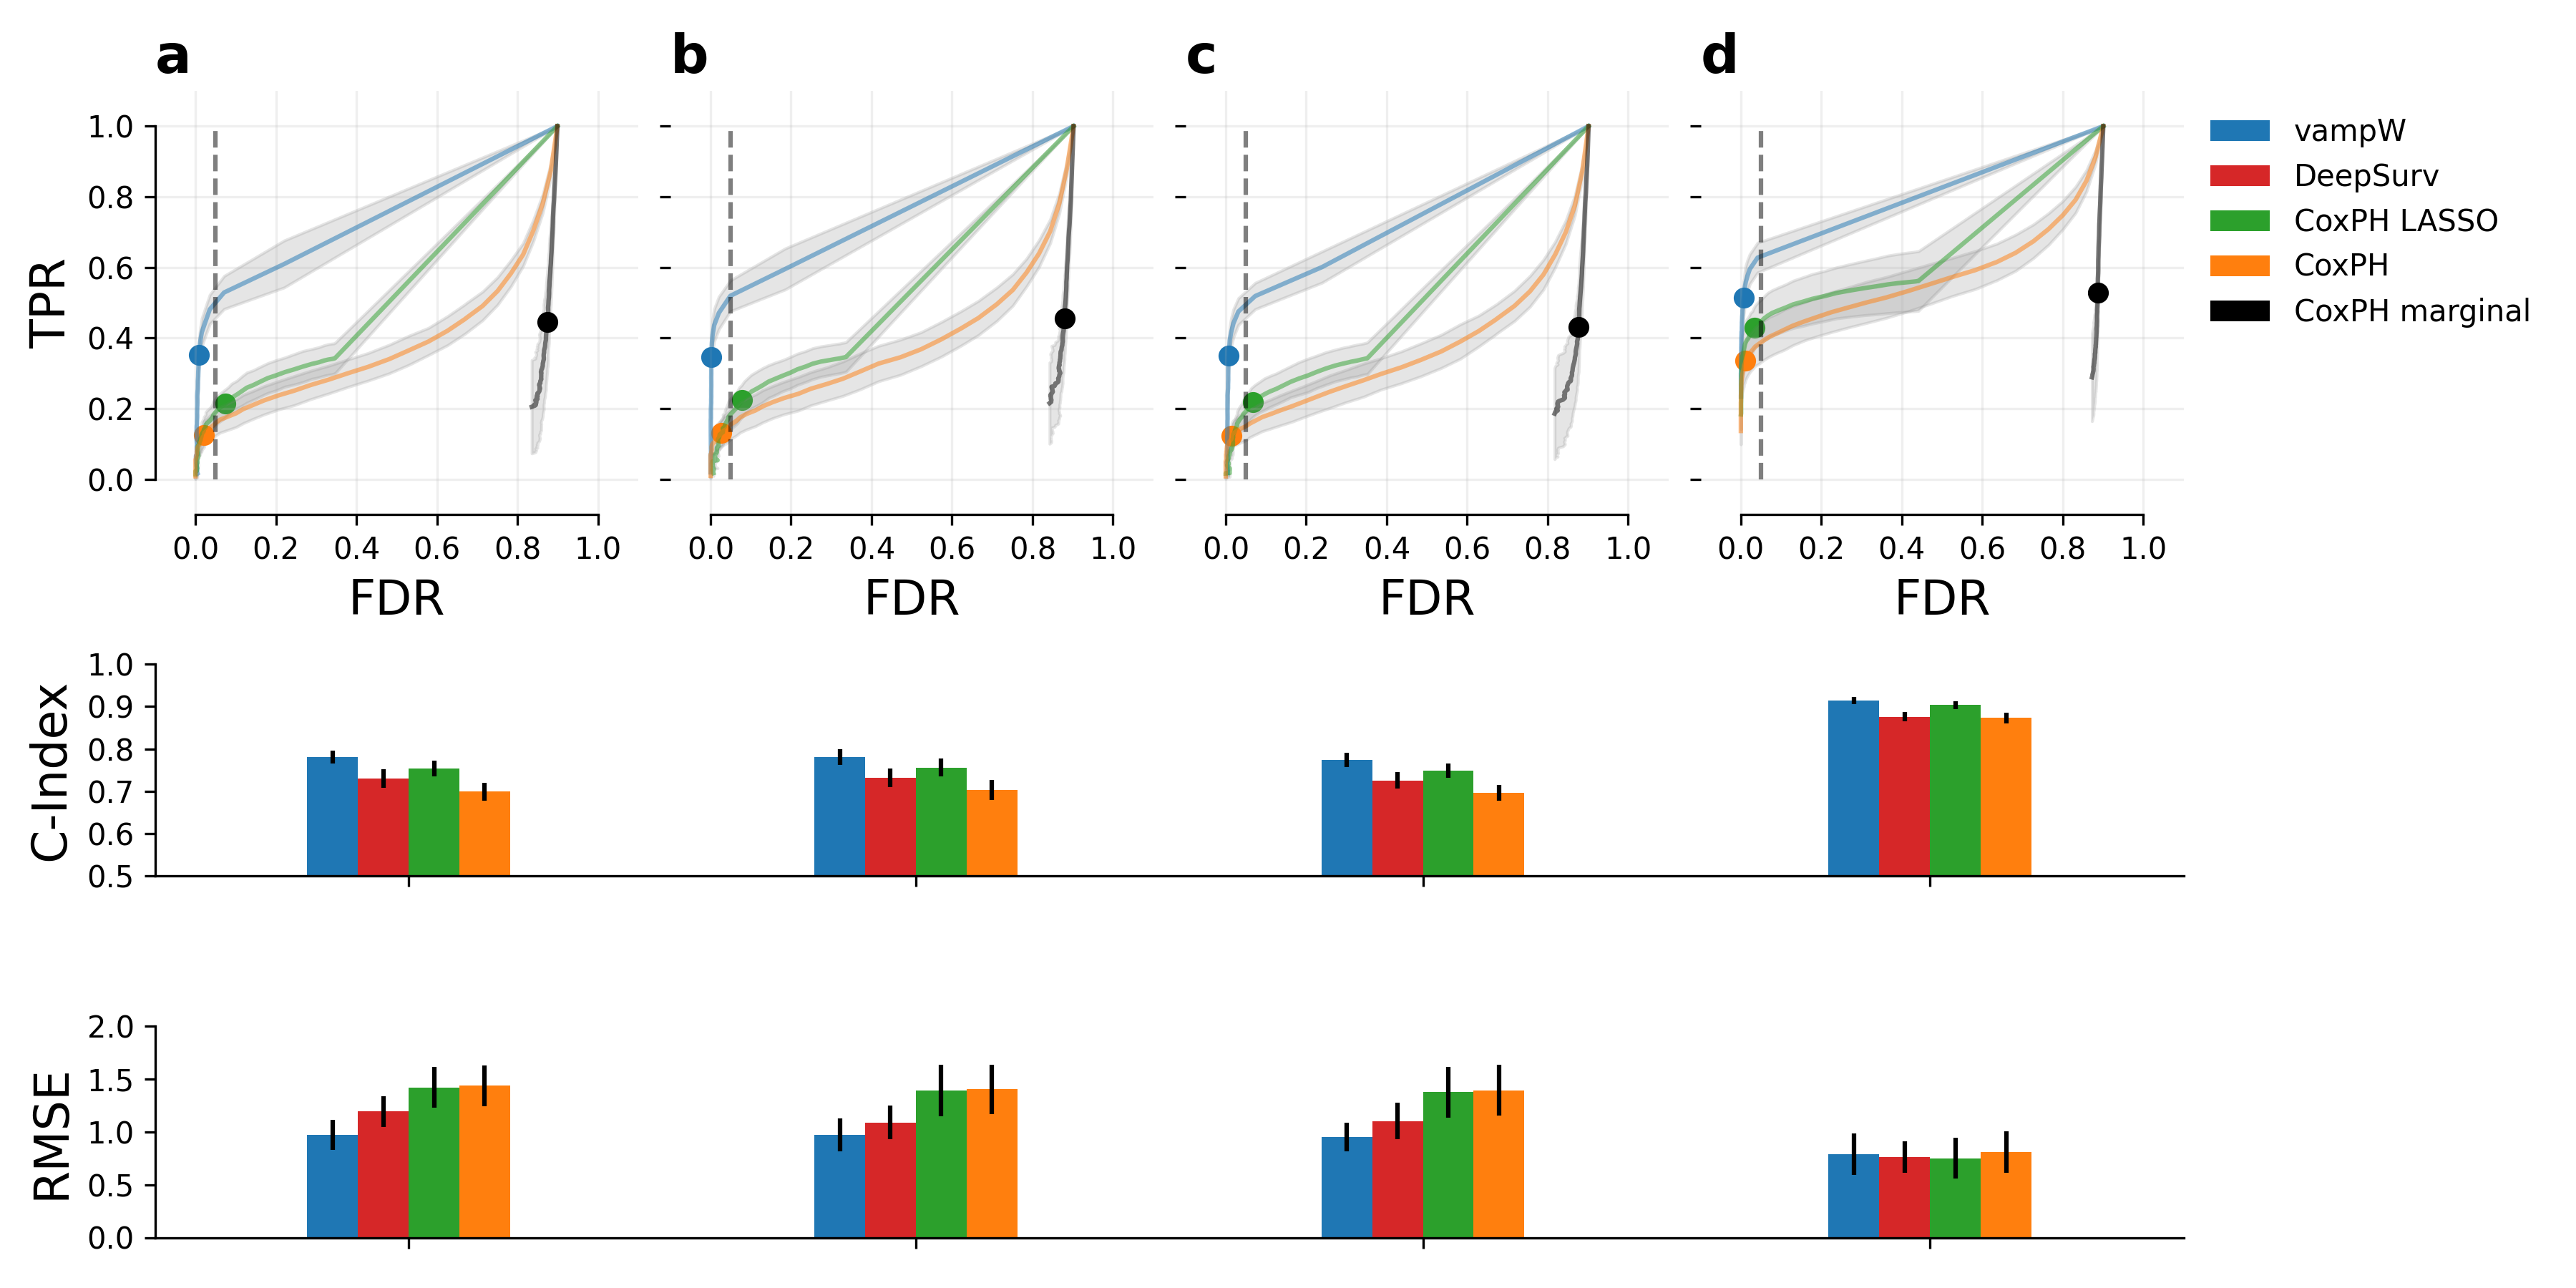
\includegraphics[width=\linewidth]{figures/panel_plot_1.png}
    \end{center}
    \caption[Simulation study of variable selection and out-of-sample prediction performance using 2,924 proteins across 53,018 individuals from the UK Biobank]{
    \textbf{Simulation study of variable selection and out-of-sample prediction performance using 2,924 proteins across 53,018 individuals from the UK Biobank.} We present four representative simulation scenarios (out of the 24 in total presented in Supplementary Figures~\ref{fig:fdr_tpr}-\ref{fig:sim_paired_differences}), covering low signal-to-noise ratios, model mis-specification, and high censoring rates. Specifically, subplots (a, b, c, d) correspond to simulation scenarios (m, o, q, t), as described in Supplementary Table \ref{tab:sim}. Across all subplots, we use the following color convention: vampW in blue, marginal CoxPH in black, joint CoxPH in orange, LASSO-penalized CoxPH in green, and DeepSurv in red. In the first row, we show variable selection performance as the relationship between \acrlong{fdr} ($\text{FDR} = \text{FP} / (\text{FP} + \text{TP}))$  and true positive rate ($\text{TPR} = \text{TP} / (\text{TP} + \text{FN}))$. For vampW, we use posterior inclusion probabilities (PIPs), while for the other methods, p-value testing across multiple thresholds is employed, see Methods for details. Colored dots indicate the 0.95 threshold for vampW PIP and the Bonferroni-corrected 0.05 threshold for the other methods. The second row presents prediction performance measured by the concordance index (C-index) on a held-out test set. The last row presents prediction performance measured by the Root Mean Squared Error (RMSE) between the true and predicted survival times in the logarithmic domain, on uncensored individuals. The error bars (black lines in the bar plots and gray shaded areas in FDR-TPR plots) represent the standard deviation across 50 simulation replicates. \label{fig:main1}} 
\end{figure}

We begin by benchmarking vampW against several state-of-the-art variable selection approaches within a semi-synthetic simulation study. Using the 2,924 observed protein levels from the UKB PPP dataset measured in 53,018 individuals, we simulate artificial phenotypic outcomes in 24 scenarios (see Methods for details). The varied parameters are: \emph{(i)} the proportion of variance explained by biological markers, \emph{(ii)} the proportion of censored individuals, \emph{(iii)} the phenotype distribution (Weibull, ExpGamma), \emph{(iv)} the prior distribution of the slab part of the regression coefficients (Normal, Laplace), and \emph{(v)} the ExpGamma distribution parameter. Each scenario is repeated 50 times to obtain independent realizations of the simulated data, and train/test splits are resampled at a 90\%/10\% ratio across these realizations. We evaluate vampW against several approaches: one-protein-at-a-time testing (CoxPH marginal); non-penalized CoxPH fitted to all markers jointly (CoxPH); joint LASSO-penalized CoxPH with cross-validation and stability selection (CoxPH LASSO); and the deep learning approach DeepSurv (see Methods for details). We assess the ability of each method to recover the simulated causal variables and the out-of-sample time-to-event observation prediction accuracy. For variable selection, we report the false discovery rate (FDR) and true positive rate (TPR) in 4 representative scenarios in Figure \ref{fig:main1}, where $\text{FDR} = \text{FP} / (\text{FP} + \text{TP})$ and $\text{TPR} = \text{TP} / (\text{TP} + \text{FN})$, with $\text{FP}$ denoting number of false discoveries, $\text{TP}$ the number of true positive discoveries, and $\text{FN}$ the number of false negative discoveries. FDR–TPR plots for all 24 simulation scenarios are reported in Supplementary Figure~\ref{fig:fdr_tpr}.

The results of Figure \ref{fig:main1} show that joint variable selection under the Weibull model of our vampW approach achieves a calibrated false discovery rate, while outperforming both marginal and joint CoxPH models in terms of true positive rate. More precisely, marginal one-at-a-time association testing using the Cox model produces over 80\% false positives across all simulated scenarios, even with a Bonferroni correction. This is due to the fact that, when testing each protein individually, correlations can inflate false discoveries as the estimated effect is confounded by other correlated proteins. Modeling the data using a single joint CoxPH model substantially reduces false positives, leading to well-calibrated association testing with a false discovery rate below 0.05\%. Joint approach reduces the pool of candidate markers for clinical testing while capturing combined or conditional effects, which may be more informative for understanding biological pathways. Furthermore, employing a LASSO-penalized CoxPH model with 5-fold cross-validation and stability selection increases power over the joint CoxPH model, while maintaining a well-calibrated false discovery rate in most scenarios. However, the TPR achieved by the LASSO-penalized CoxPH model with stability selection is still lower than that of vampW across all settings. The complete results for all the 24 simulation scenarios in Supplementary  Figure~\ref{fig:fdr_tpr} are similar to those presented in Figure \ref{fig:main1}, where overall, the TPR of vampW is higher, with comparable or improved FDR to CoxPH approaches. This holds even under model mis-specification (generalized Gamma distribution with shape parameter $\kappa \in \{0.8, 1.2\}$) or when the prior distribution of simulated regression coefficients follows a spike-and-slab prior with slab component being a Laplace distribution which has heavier tails than the Gaussian slab prior used by vampW (Supplementary Figure~\ref{fig:fdr_tpr}). 
 
We investigate the ability of vampW to recover signals from highly correlated proteins, by annotating proteins based on their correlation structure (the top 100 correlated proteins are shown in Supplementary Figure~\ref{fig:correlation}). If the correlation of a particular protein with any other protein is greater than 0.5 in terms of the absolute value of the Pearson correlation coefficient, it is categorized as a highly correlated protein, with remaining proteins categorized as low-correlated. Supplementary Figure~\ref{fig:annot} shows that, among true-positive predictions with PIP $\geq$ 0.95, the fraction of highly versus low-correlated proteins closely matches the corresponding fraction among ground-truth in the simulation. Thus, vampW has equivalent detection power across proteins of different correlation structure.

We then compare the out-of-sample prediction accuracy across approaches, using two metrics: \emph{(i)} Harrell's concordance index (C-index) \cite{harrell_evaluating_1982}, which measures the proportion of concordant pairs, defined as $\text{C-index}=(n_{c} + 0.5 \cdot n_t) / n_{a}$, where $n_{c}$ is the number of pairs which are in the same order in predictions in comparison to the observation, $n_{t}$ is the number of tied pairs, and $n_{a}$ is all possible admissible pairs; and \emph{(ii)} root mean squared error (RMSE), which represents the average error between the predicted times and the actual diagnosis times for uncensored individuals, defined as $\text{RMSE}(\bm{y}, \hat{\bm{y}})= (N^{-1} \sum_{i=1}^{N} (y_i - \hat{y}_i)^2)^{1/2}$, where $\hat{\bm{y}}$ is the predicted outcome time and $\bm{y}$ is the ground-truth for the uncensored individuals. For the simulation results (Figure~\ref{fig:main1} and Supplementary Figures~\ref{fig:sim_prediction} and ~\ref{fig:sim_paired_differences}), the RMSE is computed on $\log(\bm{y})$, which is the quantity standardized to zero mean and unit variance by all methods. For the results on real data (Figure~\ref{fig:main3}), the RMSE is computed on $\bm{y}$, which represents the actual time of onset and hence provides a more interpretable quantity.

Prediction accuracies for different methods are presented in Figure~\ref{fig:main1} for 4 representative scenarios, in Supplementary Figure~\ref{fig:sim_prediction} for all 24 simulation scenarios and in Supplementary Figure~\ref{fig:sim_paired_differences} considering pairwise differences of these performance metrics across different simulation replicas. These plots show that, in comparison to CoxPH LASSO, vampW achieves higher C-index values across all simulation scenarios, as well as lower or on par RMSE in all scenarios. We additionally compare vampW to DeepSurv, a deep learning extension of the CoxPH model developed for risk prediction. DeepSurv performs better than the standard CoxPH, but is outperformed by vampW in all simulation scenarios in terms of C-index. In terms of RMSE, in most simulation scenarios vampW and DeepSurv exhibit similar performance, with vampW being significantly better in three scenarios. We refrain from comparing association testing performance that of DeepSurv, as the latter was primarily developed for prediction tasks (in which it does not improve upon vampW) and it does not provide variable selection within the current framework. 

\subsection{Analyzing 24 disease-related outcomes in UK Biobank}

\begin{figure}[t]
    \begin{center}
    \includegraphics[width=\linewidth]{figures/panel_plot_2.png}
    \end{center}
    \caption[Protein-coding genes discovered by vampW and their genomic positions]{\textbf{Protein-coding genes discovered by vampW and their genomic positions.} The proteins discovered by vampW and their corresponding protein names that pass a posterior inclusion probability (PIP) threshold of 0.95 are shown. Disease outcomes are categorized into four groups: neurological diseases, cardiovascular diseases, cancer types, and other disease-related outcomes.\label{fig:main2}}
\end{figure}

We apply vampW to the age-at-diagnosis of 24 disease outcomes derived from medical records in the UK Biobank, linked to protein measurements from blood samples. \changed{In Figure \ref{fig:main2}, we report two sets of vampW discoveries, passing a PIP threshold of 0.95, for models with and without exponential age correction. First, for the model without exponential age correction, we also run marginal CoxPH, joint CoxPH, and LASSO-penalized CoxPH analyses, all using Bonferroni-corrected p-value testing.} Marginal testing identifies tens of times more associations compared with joint vampW testing, consistently across most traits (exceptions being Alzheimer’s disease, vascular dementia, brain/CNS disorders, and prostate disease). However, our simulation study indicates substantial inflated false discoveries when using marginal testing, which often selects features that appear significant individually but are correlated with each other, whereas joint testing produces a potentially more biologically meaningful set of discoveries, reducing the need for unnecessary follow-up experiments. The set of vampW discoveries is largely independent of the top-$x$ marginal discoveries, where $x$ corresponds to the number of vampW discoveries. Specifically, the overlap between vampW and the top-$x$ marginal CoxPH results is 37 out of 219 vampW associations. This indicates that vampW identifies largely novel associations, and that its joint testing capability cannot be replicated simply by tightening the marginal testing p-value threshold. In comparison with joint CoxPH and LASSO-penalized CoxPH, 61 and 110 associations, respectively, overlap with vampW. The overlap indicates that vampW is not overly conservative in variable selection, as it identifies proteins that are also detected by LASSO. For 9 of the 24 traits, no association passes the PIP threshold.

In the set of discoveries without exponential age correction, we highlight the discovery of collagen alpha-1(IX) \emph{COL9A1} in type 2 diabetes, which was also identified by the standard joint CoxPH model but not by CoxPH LASSO. Although it has previously been reported among top plasma proteins \cite{deng_atlas_2025}, it is not well established as a biomarker and may provide novel insights into the biological pathways underlying the disease. Another potentially novel association with type 2 diabetes is the \emph{MATN3} gene, which also exhibits an underlying interaction with \emph{COL9A1} based on text mining, as shown in Supplementary Figure~\ref{fig:interaction_networks}. Furthermore, we identify \emph{SOST} as a novel candidate associated with endometriosis, a potential biomarker that has not been widely studied in this context.

One of the leading associations we identify is the protein-coding gene \emph{CGA}, which is associated with multiple diseases, including endometriosis, T2D, depression, ischemic heart disease, liver disease, Parkinson’s disease, gynecological cancer, prostate cancer, and colorectal cancer. Notably, plasma levels of \emph{CGA} are highly influenced by age and sex in non-linear ways and rank among the top six protein-coding genes (alongside \emph{FSHB}, \emph{SOST}, \emph{GDF15}, \emph{MLN}, and \emph{PTN}) exhibiting the most significant age-dependent changes \cite{deng_atlas_2025,Sigurdsson2025}. This suggests that plasma levels of these proteins may be associated with these outcomes simply because both the proteins and the time-to-diagnosis both vary exponentially with age. 

To explore this further, we conduct an additional adjustment of the plasma protein observations including exponential age effects along with the linear ones (see Methods), and re-analyze the traits. This yields associations of plasma protein levels with disease onset beyond age-related variation. The protein-coding gene \emph{CGA}, previously reported as age-associated, disappears from ischemic heart disease, colorectal disease, and mortality associations when non-linear effects of age on protein levels are taken into account (see Figure~\ref{fig:main2} and Figure~\ref{fig:cov_age}). Moreover, for certain outcomes, the signal becomes attributed to a different set of proteins, revealing new underlying biological structure. For example, we find the chemokine \emph{CXCL17} as associated with colorectal cancer, which is previously reported as a potential biomarker for the diagnosis of colon cancer \cite{ohlsson_ectopic_2016}. Furthermore, we identify Tenascin-XB (TNXB) protein, encoded by the TNXB gene, which is recognized as a potential blood-based plasma biomarker associated with depression \cite{biomedicines8110455}. PARK7 (also known as DJ-1) is a multifunctional protein that acts as an antioxidant sensor. Its oxidized form (oxDJ-1) in blood has been proposed as a promising biomarker for early-stage Parkinson’s disease \cite{Matsuda2024ModificationsOD}. It was also identified by vampW, after exponential age correction, in association with Parkinson’s disease and rheumatoid arthritis.

Regardless of the age correction approach, we find several associations supported by recent literature. In particular, we find \emph{ACE} to be associated with both hypertension and ischemic heart disease, supporting a role in blood pressure regulation \cite{zambrano_genetic_2023}. Prostate-specific antigen (PSA) is the most widely used clinical biomarker for identifying men at risk of prostate cancer prior to symptom onset, and its mechanisms have been extensively studied \cite{pellegrino_mechanistic_2021}. PSA is encoded by the \emph{KLK3} gene, which exhibits an association with prostate cancer, regardless of age correction approach in our study. Growth differentiation factor 15 (\emph{GDF15}) reduces food intake and represents a promising therapeutic target for the treatment of type 2 diabetes \cite{aguilar-recarte_knocking_2022}. It is also a useful biomarker for identifying individuals at increased risk of diabetes \cite{aguilar-recarte_knocking_2022}, and vampW exhibits a strong association between GDF15 protein levels and type 2 diabetes. Variation in the \emph{APOE} protein, especially the alleles $\varepsilon_3$ and $\varepsilon_4$, has been widely established as a risk factor for late-onset disease across multiple large cohorts \cite{williams_proportion_2026}. Regardless of adjustment for non-linear age effects, we find \emph{APOE} to be significantly associated with Alzheimer’s disease progression. \changed{We also identify renin (REN) associated with hypertension, which is a key enzyme in the renin-angiotensin-aldosterone system (RAAS), making its measurement—often via plasma renin activity (PRA)—a crucial biomarker for classifying, diagnosing, and assessing cardiovascular risk in hypertension patients \cite{VOLPE2012312}.}

% Overall, vampW discoveries exhibit average replication rates across traits of 52\% and 73\% for models with and without exponential age correction, respectively, when compared with the DISEASES 2.0 gene–disease database at a Z-score threshold of 2, adjusted for overlap in genes and diseases between the datasets. 
We further identify 262 and 9 protein associations, respectively, for the models with and without exponential age correction that show no prior link to a given disease in the DISEASES 2.0 database, which integrates disease-gene associations from automatic text mining and is updated on a weekly basis (we use March 2026 version). We examine the total \acrfull{snp} heritability of proteins, as shown in Supplementary Figure \ref{fig:protein_h2}, using values reported in \cite{sun_plasma_2023}. We find no significant deviation of vampW-discovered proteins compared to all proteins in the study, with average SNP heritability of 19.9\% and 18.7\% for models with and without exponential age correction, respectively.

To further validate the vampW discoveries and assess whether they can be replicated in a cohort using a different sampling technology, we matched proteins and outcomes between the UK Biobank and a SomaScan v4 study of plasma samples from 36,000 Icelandic individuals \cite{eldjarn_large-scale_2023}.
% To further validate the vampW discoveries, we match proteins and outcomes between the UK Biobank and a SomaScan v4 study of plasma samples from 36,000 Icelandic individuals \cite{eldjarn_large-scale_2023}. 
Among the vampW discoveries, we identified matching proteins for Alzheimer's disease, depression, hypertension, rheumatoid arthritis, and prostate cancer. Of the 71 matched discoveries, 48 also show an association using logistic regression with binary disease occurrence in the Icelandic cohort at a Bonferroni-adjusted p-value threshold. 
% Moreover, we attempted to replicate our findings in the independent Generation Scotland (GS) study, which employed SOMAscan V.4 technology, in contrast to the Olink Explore 3072 PEA platform used in UK Biobank. We observed limited overlap in the proteins measured across the two studies, as well as a low prevalence of certain diseases of interest, making replication challenging. Nevertheless, we successfully replicated the association of CDH5 with hypertension, a protein recently recognized as a key contributor to hypertension pathogenesis \cite{aldisi_identification_2025}.

\begin{figure}[t]
    \begin{center}
    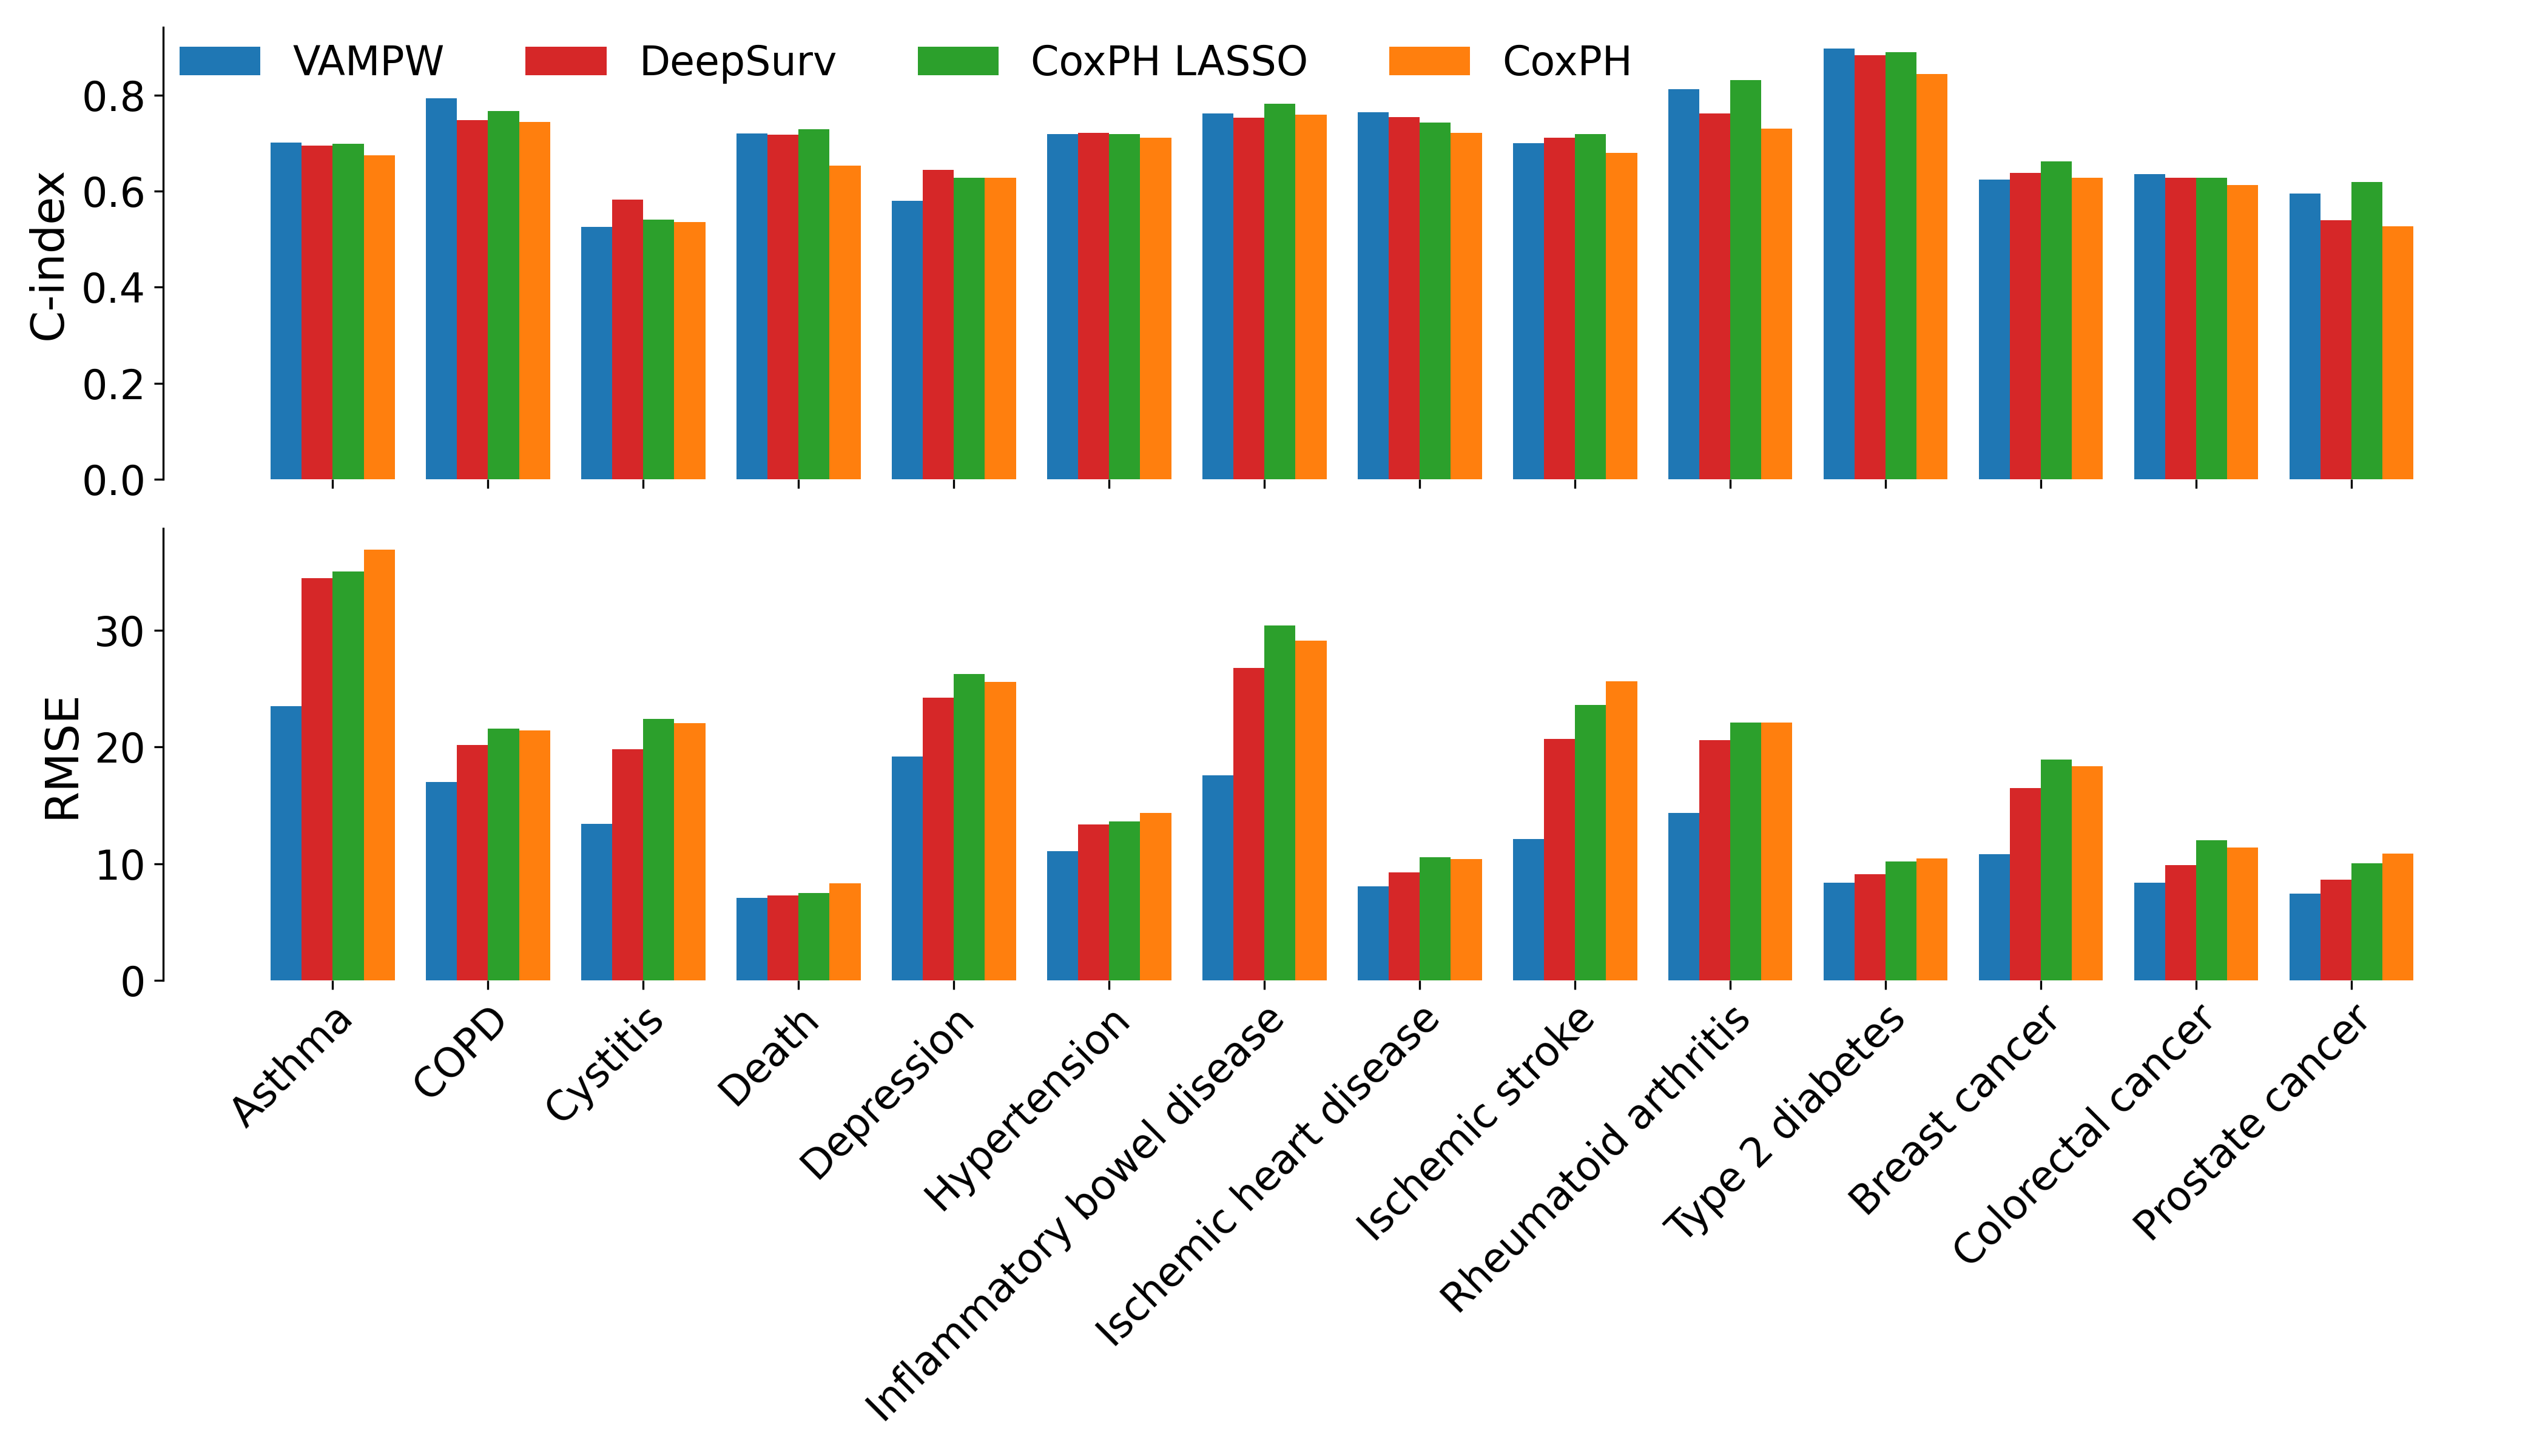
\includegraphics[width=\linewidth]{figures/panel_plot_3.png}
    \end{center}
    \caption[Out-of-sample performance comparison for CoxPH, LASSO-penalized CoxPH, DeepSurv, and vampW]{
    \textbf{Out-of-sample performance comparison for CoxPH, LASSO-penalized CoxPH, DeepSurv, and vampW.} 
    We evaluate time-to-diagnosis predictions for 14 health-related outcomes in the UK Biobank (traits with $\ge 100$ cases in the test set) using protein measurements adjusted for age and sex. 
    Model accuracy is assessed using the Concordance Index (C-index), which measures the probability of correctly ranking patient risks, and the root mean squared error (RMSE), representing the average error in years between predicted and actual diagnosis times for uncensored individuals. Training is performed on data that is first log-transformed and standardized to zero mean and unit variance, and then scaled back using an exponential transformation. To represent actual survival times, we rescale the predictions back to years using statistics from the training set. A sensitivity analysis shows that using test-set statistics for this rescaling impacts results negligibly and preserves the ordering of methods in terms of their performance. In terms of RMSE, vampW significantly improves over all other methods. In terms of C-index, vampW outperforms CoxPH, and it performs on par with CoxPH LASSO and DeepSurv.
  }
    \label{fig:main3}
\end{figure}

In Figure \ref{fig:main3}, we show the absolute values of C-index and RMSE metrics across traits with more than $100$ uncensored individuals (representing cases) present in the test set. In terms of RMSE, vampW outperforms all other methods across all traits: on average, it reduces the RMSE by 33\% with respect to CoxPH, by 32\% with respect to CoxPH LASSO and by 26\% with respect to DeepSurv. Figure~\ref{fig:main3} gives the RMSE in the actual scale of years, and we also present the RMSE in the logarithmic time domain, assuming standardized $\log(\bm{y})$, in Supplementary Figure~\ref{fig:real_rmse_time}, which shows that the relative performance ranking of the methods remains unchanged.

In terms of out-of-sample C-index performance, vampW shows an improvement over CoxPH in $11/14$ traits, over LASSO-penalized CoxPH in $6/14$ traits and over DeepSurv in $9/14$ traits. Furthermore, on average, the C-index of vampW is 0.5\% better than that of DeepSurv, 4\% better than that of CoxPH, and 1.3\% worse than that of LASSO-penalized CoxPH. Finally, we note that the largest deviations from the Weibull distribution, as shown in Supplementary Figure \ref{fig:distance}, occur for asthma and inflammatory bowel disease, for which vampW has limited power for association testing but still demonstrates improved time-prediction performance over the various baselines. In comparison to other methods, vampW yields better prediction performance at later ages for most outcomes, based on the Brier score, as shown in Supplementary Figure~\ref{fig:bs_t75}.

We find that vampW generates highly transferable protein risk scores across diverse genetic ancestries, maintaining predictive utility in minority populations. Specifically, while vampW achieves comparable accuracy in terms of C-index to CoxPH LASSO, it consistently outperforms both standard CoxPH and CoxPH LASSO models in minimizing overall prediction error (RMSE), as seen in Supplementary Figure~\ref{fig:genetic_ancestry_exp_50_10}.

To demonstrate the wider applicability of our algorithm outside the proteomics domain, we additionally benchmark vampW in data-scarce regimes using common survival benchmarking datasets, following the study \cite{monod_neuralsurv_2025}. As shown in Supplementary Figure~\ref{fig:deep_benchmark}, vampW outperforms all deep learning methods on the METABRIC, SUPPORT, and SAC3 datasets, and outperforms 6 out of 13 benchmarking methods on the GBSG dataset. 

\section{Discussion}
In this work, we develop the novel vampW algorithm for Bayesian variable selection under the Weibull model. Applying our approach to the largest proteomics data available to date, we demonstrate its capability to jointly fit thousands of plasma proteomics markers across tens of thousands of individuals from the UK Biobank, revealing new disease biomarkers. Our simulation study shows that vampW outperforms state-of-the-art methods for variable selection, reducing false discoveries compared to marginal testing and improving the true positive rate relative to multiple forms of CoxPH models. When analyzing real health-related outcomes from the UK Biobank, vampW identifies 219 associations between protein levels and human complex diseases. Our discoveries exhibit a 68\% replication rate in an independent Icelandic cohort, accounting for overlap in proteins and outcomes between the studies. 

vampW provides point estimates of the posterior mean, and its prediction performance is expected to be Bayes-optimal. For out-of-sample prediction of the outcome ranking (C-index), vampW outperforms the standard CoxPH model and achieves performance comparable to penalized versions of CoxPH and to the deep learning-based method DeepSurv. For the prediction of disease onset times in uncensored individuals, vampW yields more accurate predictions, measured by RMSE, as compared to all other benchmarked methods. We also show that vampW generates highly transferable protein risk scores across diverse genetic ancestries and achieves strong out-of-sample prediction performance in other non-proteomics data-scarce regimes, outperforming deep learning methods on most of the examined survival benchmarking datasets, even when trained on very small sample size. 

There are several limitations and potential avenues for future work. First, plasma protein levels, as well as other multi-omics markers, may be influenced by multiple confounding factors, such as medication use, sex, and age, including non-linear effects of age on protein levels, as suggested by our ablation study. In this context, a key direction for future work is to leverage the medical records of individuals in the UK Biobank, which would allow adjustments for a broader set of potential confounders. Moreover, to examine whether variation in protein levels reflects disease predisposition or the disease state itself, one possible approach is to restrict the analysis to individuals who experience events after the date of blood sampling and assessment, rather than incorporating both prospective and historical events. With more samples available, covering a larger portion of the population prevalent with a certain disease, studying associations between survival time and protein levels during the follow-up period represents a viable approach. Additional extensions are models that can identify relevant age-related changes in protein levels that are associated with disease onset at different time points, which requires repeated proteomics observations.

In terms of model stability, although the UKB PPP protein design matrix violates the assumptions required for Bayes optimality of our algorithm, introducing damping and damping autotuning (see Methods) empirically results in strong predictive performance. The damping choices affect the convergence properties when searching over the parameter space, as too strong damping may cause the algorithm to get stuck in local minima; and thus we propose a grid search of starting parameters which is facilitated by the efficient implementation of our algorithm (see Methods). 

% \marco{this paragraph does not seem to belong here, but would be better suited for Methods?}


Finally, our future work will also focus on improving the computational efficiency of the vampW algorithm through parallelization and reduced memory requirements, which has the potential to enable large-scale analyses involving hundreds of thousands of omics markers.  

In summary, vampW is a novel approach for selecting multiomic biomarkers associated with human diseases and for predicting disease onset times. With increasing sample sizes and expanding data coverage in the world’s largest biobanks, joint vampW analyses have the potential to advance our understanding of the genomic architecture of complex human diseases by enabling interpretable identification of disease associations and providing accurate predictions of disease onset.

\section{Methods}
\subsection{Weibull model for time-to-event outcomes}\label{subsec:W}

We consider a Weibull$(\alpha, \eta)$ model, one of the most common models in survival analysis, where $\alpha$ and $\eta$ are the shape and scale parameters. We follow a recently proposed formulation of the model~\cite{Ojavee2021-zu}, where we aim to estimate mean and variance of the time-to-event outcome. Let $y_i$ be the time at which the individual $i$ experiences the event, and consider the survival function $S(y_i) = \exp(-(\frac{y_i}{\eta_i})^{\alpha})$. In the logarithmic space, the mean and variance of the model can be separated as follows:
\begin{align}
    & \mathbb{E}[\log(y_i)] = \log(\eta_i) - \frac{K}{\alpha}, \\
    & \text{Var}[\log(y_i)] = \frac{\pi^2}{6 \alpha^2},
\end{align}
where $K$ is the Euler-Mascheroni constant ($\approx 0.57722$). Once the variance is independent of the scale parameter $\eta_i$, one can introduce the vector of underlying latent genetic effects $\bm{\beta}$ as $\bm{\eta} = \exp(\mu + \bm{X} \bm{\beta} + \frac{K}{\alpha})$, resulting in $\mathbb{E}[\log(\bm{y})] = \mu + \bm{X} \bm{\beta}$, where $\bm{X} \in \mathbb{R}^{N \times P}$ is a design matrix containing observations on $N$ individuals and $P$ biological markers, $\bm{y}=[y_1, \ldots, y_N]$, $\bm{\eta}=[\eta_1, \ldots, \eta_N]$, $\bm{\beta}$ is the vector of marker effects, and $\mu$ represents the model intercept. The columns of the matrix $\bm{X}$ are normalized, i.e., they each have zero mean and unit variance. Using the fact that the logarithm of a Weibull random variable follows a Gumbel distribution and the Location-Scale property of the Gumbel distribution, we formulate the final model as
\begin{equation}
    \label{eq:vampW_model}
    \log (\bm{y} )=\mu + \bm{X} \bm{\beta} + \frac{\bm{w}}{\alpha} + \frac{K}{\alpha}, 
\end{equation}
where $\bm{w} = [w_1, \dots, w_N]$ with each $w_i$ following the Gumbel$(0,1)$ distribution. We note that in the algorithm and software described below, any arbitrary measurement represented in floating point can be accommodated as the entries of $\bm{X}$. These can be gene expression, methylation, copy number variants, DNA sequence variation, protein measures, which can all be included alongside one another. 

To allow for a range of effect sizes from different data types, we select the prior on the marker effects $\bm{\beta}$ to be distributed as a form of spike and slab distribution, with non-zero signals coming from a mixture of normal distributions,
\begin{equation}
\label{eq:prior}
    \beta_j \sim ( 1 - \lambda ) \delta_0 + \lambda \sum^L_{i=1} \pi_i \cdot \mathcal{N}(0, \sigma^2_i),
\end{equation}
where $(\pi_1, \dots, \pi_L)$ denotes the vector of inclusion probabilities for each of the $L$ mixture components, $\delta_0$ is a Dirac spike function at 0, $\lambda$ is the sparsity ratio, and $(\sigma^2_1, \dots, \sigma^2_L)$ are mixture-specific variances.

Finally, we account for the right-censoring issue inherent in time-to-event data. In practical applications, the true event time $y_i$ is often right-censored, meaning that the event of interest has not occurred for some individuals by the end of the study. Consequently, we do not observe $y_i$ directly for all $i$; instead, we observe the time $\min(y_i, C_i)$ and an indicator $\delta_i = \mathbb{I}(y_i \leq C_i)$, where $C_i$ is the censoring time and $\delta_i=1$ implies the event was observed while $\delta_i=0$ implies it was censored.

\subsection{vampW algorithm and its implementation}\label{sec:vampW}

To infer the parameters of Equations \eqref{eq:vampW_model} and \eqref{eq:prior}, we propose an algorithm that we call vampW, which is based on Vector Approximate Message Passing (VAMP) for generalized linear models \cite{rangan_vector_2019, schniter_vector_2016}, where the outcome variable is observed through a noisy and non-linear Weibull channel. It adaptively estimates the prior-specific parameters $\Theta = \{\lambda, (\pi_i)_{i=1}^L, (\sigma_i^2)_{i=1}^L \}$ via a Bayesian Expectation-Maximization procedure, as introduced in EM-VAMP \cite{LearningFreeEnergies2018}. vampW introduces a novel approach for handling censored data, as well as denoisers derived specifically for Weibull link functions and the corresponding expectation-maximization updates. We highlight that no existing AMP method is able to address the challenge of censored data. 
% \marco{unnatural rendering: lots of blank space in this page and in the next page the page number displays in the middle of the algorithm. Please fix.}

As seen in Algorithm \ref{alg:vampW}, vampW consists of two denoising steps and two (non-linear) minimum mean-squared error (MMSE) estimation steps, applied separately to the vector of effect sizes $\bm{\beta}$ and to the latent predictor. The denoising step accounts for the prior properties of the model when considering a noisy estimate of either  $\bm{\beta}$ or the latent predictor, while the MMSE step further refines the estimates by taking the correlation structure among the columns in the design matrix $\bm{X}$ into account. The key feature is the so-called \textit{Onsager correction}, which is added to ensure the asymptotic normality of the noise corrupting the algorithm's estimates of $\bm{\beta}$ at every iteration, important for the subsequent feature selection. A direct application of generalized EM-VAMP to real genomics, epigenetics and proteomics measures may lead to signal-estimation divergence, primarily due to violations of right-rotational invariance in the data design matrix, one of the assumptions in the original EM-VAMP algorithm. To mitigate these stability issues, damping is applied to the denoised signals---a standard practice in practical EM-VAMP implementations \cite{VAMP_MRI,sarkar2021mri}---as seen on line 11 of Algorithm \ref{alg:vampW}, where $\rho \in ( 0, 1 )$ denotes the damping factor.
% To mitigate these stability issues, we perform \emph{damping} of denoised signals, as seen on line 11 of Algorithm \ref{alg:vampW}, where $\rho \in ( 0, 1 )$ denotes the damping factor. 

% \begin{algorithm}[H]
% % \begin{breakablealgorithm}
%     \caption[Vector Approximate Message Passing for Weibull Model]{vampW}
%     \label{alg:vampW}
%     \scriptsize     
%     % Rescale the algorithm to 90% of its original size to fit on the page
%     % \scalebox{1.1}{
%         % \begin{minipage}{1.38\linewidth} % Adjust minipage width to compensate for scaling (1/0.85 approx 1.17)


    %%%%%%%%%%%%%%%%%%%%
    % \begingroup
    % \vspace{1em}
    % \hrule height 0.8pt
    % \vspace{0.5em}

    % % Using algocf integrates perfectly with algorithm2e!
    % \captionof{algocf}[Vector Approximate Message Passing for Weibull Model]{vampW}
    % \label{alg:vampW}

    % \vspace{0.5em}
    % \hrule
    % \vspace{0.5em}

  % We use a group to keep the spacing contained
\begin{breakablealgorithm}{Vector Approximate Message Passing for Weibull Model}{vampW}{alg:vampW}
    \begin{algorithmic}[1]
    % \addtolength{\leftskip}{1.5em}
    \STATE {\bfseries Input:} max number of iterations $N_{it}$, \\ 
    normalized design data matrix of uncensored individuals $\boldsymbol{X} \in \mathbb{R}^{N \times P}$, \\
    normalized design data matrix of censored individuals $\bm{X}_{\mathcal{C}} \in \mathbb{R}^{N_{\mathcal{C}} \times P}$, \\
    vector of measured phenotypes $\bm{y} \in \mathbb{R}^N$, \\
    vector of censoring times $\bm{y}_{\mathcal{C}} \in \mathbb{R}^{N_{\mathcal{C}}}$,\\
    initial noisy signal estimate $\bm{r}_{10} \in \mathbb{R}^P$, 
    \\ 
    initial signal precision estimate $\gamma_{10} > 0$, \\ 
    initial noisy genetic predictor estimate $\bm{p}_{10} \in \mathbb{R}^N$,
    \\ 
    initial genetic predictor precision estimate $\tau_{10} > 0$, \\
    initial set of parameters defining prior distribution $\Theta_{0}$, \\ 
    initial estimate of Weibull model hyperparameters $\mu \in\mathbb{R}$ and $\alpha > 0$,\\ 
    damping factor $\rho$, \\
    damping reduction factor $c_{\rho} < 1$, \\
    max damping autotune steps $N_{\rho\_steps}$, \\
    flag to enable damping autotuning
    \FOR{$t = 0, 1,\dots, N_{\text{it}}$ 
    }
        \STATE {\bfseries Denoising of the effect sizes}
        \STATE { \text{EM} update of the prior distribution parameters $\Theta$, called $\Theta_t$} 
        
        \STATE $\hat{\bm{\beta}}_{\text{new}} = \mathbb{E}[\bm{\beta} | \bm{r}_{1t} = \bm{\beta} + \mathcal{N}(0, \gamma_{1t}^{-1}\bm{I}), \gamma_{1t}, \Theta_{t}]$
        %\footnotemark \marco{unclear what footnote is doing here}
        
        \IF {$t=0$}
            \STATE $\hat{\bm{\beta}}_{1t} = \hat{\bm{\beta}}_{\text{new}}$
        \ELSE
            \IF {damping autotuning is enabled}
                \FOR{$k = 1, \dots, N_{\rho\_steps}$}
                    \STATE $\hat{\bm{\beta}}_{1t} = \rho \cdot \hat{\bm{\beta}}_{\text{new}} + (1-\rho) \cdot \hat{\bm{\beta}}_{1t-1}$
                    \IF {$\text{C-index}_{\textbf{train}}(\hat{\bm{\beta}}_{1t}) \ge \text{C-index}_{\textbf{train}}(\hat{\bm{\beta}}_{1t-1})$}
                        \STATE \textbf{break}
                    \ELSE
                        \STATE $\rho \leftarrow \rho \cdot c_{\rho}$
                    \ENDIF
                \ENDFOR
            \ELSE
                \STATE $\hat{\bm{\beta}}_{1t} = \rho \cdot \hat{\bm{\beta}}_{\text{new}} + (1-\rho) \cdot \hat{\bm{\beta}}_{1t-1}$
            \ENDIF
        \ENDIF

        \STATE $\alpha_{1t} = \gamma_{1t} \cdot \langle \text{Var}[\bm{\beta}|\bm{r}_{1t} = \bm{\beta} + \mathcal{N}(0, \gamma_{1t}^{-1}\bm{I}), \gamma_{1t}, \Theta_{t}] \rangle$ %\footref{formula:denoiser}
        \STATE $\gamma_{2t} = \gamma_{1t} \cdot (1 - \alpha_{1t}) / \alpha_{1t}$ 
        \STATE $\bm{r}_{2t} = (\hat{\bm{\beta}}_{1t} - \alpha_{1t} \bm{r}_{1t}) / (1-\alpha_{1t})$
        \item[]
        \STATE {{\bfseries Denoising of the genetic predictor }(see Section \ref{sec:sup1})}
        \STATE $\hat{\bm{z}}_{1t} = g_z(\bm{p}_{1t}, \tau_{1t})$

        \STATE $\upsilon_{1t} = \langle \tau_1 / ( \tau_1 + \alpha^2 \bm{y}^\alpha \cdot e^{-\alpha(\mu+\hat{\bm{z}}_{1t}) - K}) \rangle$
        \STATE $\tau_{2t} = \tau_{1t} \cdot (1 - \upsilon_{1t}) / \upsilon_{1t}$ 
        \STATE $\bm{p}_{2t} = (\hat{\bm{z}}_{1t} - \upsilon_{1t} \bm{p}_{1t}) / (1-\upsilon_{1t})$
        \item[]
        \STATE { EM update of the estimates of Weibull model hyperparameters $\alpha$ and $\mu$ (see Section \ref{sec:sup3})} 
            
        \STATE \textbf{Nonlinear censoring MMSE of the effect sizes} (see Section \ref{sec:sup2})

        \STATE $\hat{\bm{\beta}}_{2t}^{(0)} = ( \tau_{2t} \bm{X}^\top\bm{X} + \gamma_{2t} \bm{I} )^{-1} ( \tau_{2t} \bm{X}^\top \bm{p}_{2t} + \gamma_{2t} \bm{r}_{2t} )$ 
        \STATE Compute $\hat{\bm{\beta}}_{2t}$ by solving $F(\bm{\beta}) = 2 \gamma_{2t} \bm{r}_{2t} + 2 \tau_{2t} \bm{X}^\top \bm{p}_{2t}$ with initialization $\bm{\beta}_{init} = \hat{\bm{\beta}}_{2t}^{(0)}$, where \newline
            % F(beta) in one unbreakable two-line block, so it is not split across lines or pages.
            \quad \quad $\begin{aligned}[t] F(\bm{\beta}) & = 2(\gamma_{2t}I + \tau_{2t}\bm{X}^\top\bm{X})\bm{\beta} \\ & \quad - \alpha \bm{X}_\mathcal{C}^\top \text{exp}\Big(\alpha(\log(\bm{y}_\mathcal{C}) - \mu - \bm{X}_\mathcal{C} \bm{\beta})-K\Big) \end{aligned}$

        \STATE $\alpha_{2t} = 2 \gamma_{2t} \cdot \text{Trace}([J_{\beta}F(\hat{\bm{\beta}}_{2t})]^{-1})/P$, where $J_{\beta} F(\bm{\hat{\beta}}_{2t}) = 2(\gamma_{2t} \bm{I} + \tau_{2t}\bm{X}^\top\bm{X}) + \nabla^2 g(\hat{\bm{\beta}}_{2t})$ 
        \STATE $\gamma_{1,t+1} = \gamma_{2t} \cdot (1-\alpha_{2t}) / \alpha_{2t}$
        \STATE $\bm{r}_{1,t+1} = (\hat{\bm{\beta}}_{2t} - \alpha_{2t} \bm{r}_{2t}) / (1-\alpha_{2t})$ 
            
        \item[]
        \STATE \textbf{MMSE of the latent predictor}

        \STATE $\hat{\bm{z}}_{2t} =  \boldsymbol{X} \hat{\bm{\beta}}_{2t}$ 
        \STATE $\upsilon_{2t} = 2 \cdot \tau_{2t} \cdot \text{Trace}(\bm{X} \cdot [J_{\beta}F(\hat{\bm{\beta}}_{2t})]^{-1} \cdot \bm{X}^\top)/ N$
        \STATE $\tau_{1,t+1} = \tau_{2t} \cdot (1 - \upsilon_{2t}) / \upsilon_{2t}$ 
        \STATE $\bm{p}_{1,t+1} = (\hat{\bm{z}}_{2t} - \upsilon_{2t} \bm{p}_{2t}) / (1 - \upsilon_{2t})$
    
    \ENDFOR
    \STATE \textbf{return} $\hat{\bm{\beta}}_{1t}$
    \end{algorithmic}
\end{breakablealgorithm}

This approach makes the algorithm take smaller steps when learning $\bm{\beta}$. In order to further stabilize convergence and improve prediction performance, we employ damping autotuning \cite{VAMP_MRI,sarkar2021mri}: we iteratively reduce the damping by the factor $c_{\rho}$ while the training prediction, using signal estimates from the denoising step $\hat{\bm{\beta}}_1$, increases over the last iteration, measured by the concordance index (C-index), as seen in line 12 of Algorithm \ref{alg:vampW}. Following recent implementation tailored to genomic data \cite{Depope2026}, we employ the Hutchinson estimator introduced in \cite{Hutchinson} and applied to EM-VAMP in \cite{schniter2021gampmatlab} to evaluate the trace of the inverse of regularized Gram matrices, and we warm-start the conjugate gradient (CG) algorithm approximating the solution of the linear system (line 32 in Algorithm \ref{alg:vampW}). The CG solver %in subsequent VAMP iterations 
is initialized from the value at convergence in the previous iteration, which leads to reduced computational time. Compared to the gVAMP algorithm introduced by \cite{Depope2026} for a linear model without censoring, vampW derives a non-linear Weibull model within the AMP framework and incorporates censoring information into the process (as detailed in the paragraph below), thus requiring two denoising steps and two non-linear MMSE estimation steps.

\subsubsection{Handling right censorship with vampW}
As disease outcomes are only partially observed, with data being frequently right-censored, we revise the LMMSE formulation of the standard VAMP algorithm for generalized linear models to explicitly incorporate the censored phenotypes. Let $\mathcal{C} = \{i \mid \delta_i = 0\}$ denote the set of indices corresponding to the $N_{\mathcal C}$ censored individuals ($|\mathcal C|=N_{\mathcal C}$), $\bm{y}_\mathcal{C}=[y_{c, 1}, \ldots, y_{c, N_{\mathcal C}}]\in \mathbb R^{N_{\mathcal C}}$  the censored observations and $\bm{z}_\mathcal{C} = \bm{X}_\mathcal{C} \bm{\beta}$ the corresponding linear predictors, where $\bm{X}_\mathcal{C}$ represents the matrix containing only information on individuals in $\mathcal{C}$. We note that both the data matrix and the phenotype vector are split into censored and uncensored individuals at runtime, without the need to perform the splits manually beforehand. 

We reformulate the problem by incorporating the survival function of the standard Gumbel distribution $S_w$ into the likelihood term of the optimization problem. We recall that the survival function of the standard Gumbel distribution evaluated at $\alpha\left(\log(y_{c,i}) - \mu - (\bm{X}_\mathcal{C} \bm{\beta})_i \right) -K$ reflects the probability that the censored individual $i$ survived longer than the censoring time $y_{c, i}$. Relying on the state evolution result that noisy version of the signal and genetic predictor behave as $\bm{r}_{2t} \sim \mathcal{N}(\bm{\beta},\gamma_{2t}^{-1}\bm{I})$ and $\bm{p}_{2t} \sim \mathcal{N}(\bm{X}\bm{\beta},\tau_{2t}^{-1}\bm{I})$, and motivated by the previous interpretation, the final optimization task at hand becomes:

\begin{equation}
\label{formula:cenosring_opt_problem}
\begin{split}
& \hat{\bm{\beta}}_{2t} = \operatorname*{arg\,min}_{\bm{\beta} \in \mathbb{R}^P} \Bigg\{ \gamma_{2t} \| \bm{r}_{2t} - \bm{\beta} \|_2^2 + \tau_{2t} \| \bm{p}_{2t} - \bm{X} \bm{\beta} \|_2^2 \\
& \qquad - \sum_{i=1}^{N_{\mathcal C}} \log S_w\left(\alpha\left(\log(y_{c,i}) - \mu - (\bm{X}_\mathcal{C} \bm{\beta})_i \right) -K \right) \Bigg\}.
\end{split}
\end{equation} 
This objective function represents a Maximum A Posteriori (MAP) estimator for the current VAMP iteration. The quadratic terms incorporate the extrinsic information passed from the VAMP factor graph (approximated as Gaussian priors with precisions $\gamma_{2t}$ and $\tau_{2t}$), while the logarithmic term explicitly handles the non-Gaussian nature of the censored data by maximizing the survival probability $S$ for the unobserved event times. Following the derivation described in Section \ref{sec:sup2}, we obtain the following formulae for the Onsager correction terms at iteration $t$: 
\begin{align}
    \begin{split}
    \alpha_{2t} & = \frac{2 \cdot \gamma_{2t} \cdot \text{Trace}([J_{\bm{\beta}}F(\hat{\bm{\beta}}_{2t})]^{-1})}{P} \quad \text{and} \\
    \upsilon_{2t} & = \frac{2 \cdot \tau_{2t} \cdot \text{Trace}(\bm{X} \cdot [J_{\bm{\beta}}F(\hat{\bm{\beta}}_{2t})]^{-1} \cdot \bm{X}^\top)}{N},
    \end{split}
\end{align}
where $F:\mathbb{R}^P \to \mathbb{R}^P$ is defined as

\begin{align}
    \begin{split}
    F(\bm{\beta}) & = 2(\gamma_{2t}\bm{I} + \tau_{2t}\bm{X}^\top\bm{X})\bm{\beta} \\
    & \quad - \alpha \bm{X}_\mathcal{C}^\top \exp\left(\alpha(\log(\bm{y}_\mathcal{C}) - \mu - \bm{X}_\mathcal{C} \bm{\beta})-K\right),
    \end{split}
\end{align}
so that the minimizer $\hat{\bm{\beta}}_{2t}$ of \eqref{formula:cenosring_opt_problem} solves $F(\bm{\beta}) = 2 \gamma_{2t} \bm{r}_{2t} + 2 \tau_{2t} \bm{X}^\top \bm{p}_{2t}$.

\subsubsection{Association testing}
\label{sec:methods_assoc}
To evaluate the statistical relevance of the markers and test their associations with the traits under investigation, vampW provides Bayesian Posterior Inclusion Probabilities (PIPs). Following Algorithm \ref{alg:vampW}, PIPs are calculated using the noisy signal estimates $\bm{r}_{1,t}$ and the associated precision $\gamma_{1,t}$ at  iteration $t$, relying on the interpretation of those quantities within AMP frameworks in the standard setting with no censoring. We employ the PIP formulation in \cite{Depope2026}, i.e.,
\begin{equation}
    \zeta_j := \frac{\lambda_t \sum_{i=1}^L \pi_{i,t}\, \mathcal{N}\big((\bm{r}_{1,t})_j; 0, \sigma_{i,t}^2 + \gamma_{1,t}^{-1}\big)}{\lambda_t \sum_{i=1}^L \pi_{i,t}\, \mathcal{N}\big((\bm{r}_{1,t})_j; 0, \sigma_{i,t}^2 + \gamma_{1,t}^{-1}\big) + (1-\lambda_t)\, \mathcal{N}\big((\bm{r}_{1,t})_j; 0, \gamma_{1,t}^{-1}\big)},
\end{equation}
where $\zeta_j$ is the posterior probability that marker $j$ has a non-zero effect, and $\{\lambda, \allowbreak (\pi_i)_{i=1}^L, \allowbreak (\sigma_i^2)_{i=1}^L \}$ are prior parameters (Equation \ref{eq:prior}) adaptively learned throughout the vampW iterations. The PIP can be viewed as the Bayesian analogue of a p-value. We use a PIP threshold of 0.95, which represents strong evidence that a variable is associated with the outcome and corresponds to a 5\% probability of false discovery in a calibrated setting.

\subsubsection{Computational efficiency} 
vampW can be run as a single-threaded program on an HPC cluster, requiring approximately 64 GB of random-access memory (RAM) per trait and an average of 12.7 CPU hours (measured on AMD EPYC 9654 Processor) to complete a single trait analysis. This corresponds to approximately 7.3 GBP when run on a cloud-computing DNAnexus virtual machine (mem3\_ssd3\_x8)\footnote{\url{https://documentation.dnanexus.com/developer/api/running-analyses/instance-types}}, which is required due to data protection. The CoxPH LASSO approach can be parallelized, requiring a total of 160 GB of RAM when using 10 parallel CPU cores. With an average of 60.8 CPU hours required per trait, this corresponds to 10.5 GBP per trait when run on a mem3\_ssd3\_x24 machine. In comparison, CoxPH requires an average of 0.3 CPU hours per trait, and marginal CoxPH requires 0.1 CPU hours per trait, however those methods score lowest in our benchmarks in out-of-sample prediction and variable selection as we show in the Results.

\subsection{UK Biobank protein data and time-to-event phenotypes}
\label{subsection:ukb}
To validate our proposed approach, we analyze protein measures from the UK Biobank Pharma Proteomics Project (PPP) dataset \cite{sun_plasma_2023}. We use a total of 2,924 unique proteins measured across 53,018 individuals, obtained using the antibody-based Olink Explore 3072 PEA. We standardize each protein vector across individuals (ignoring missing values) to obtain zero mean and unit variance, and then impute the missing values with zeros. We adjust the protein levels by regressing them on the covariates ${\rm sex}$ and ${\rm age}$ via the linear model $\alpha_1 \cdot {\rm sex} + \alpha_2 \cdot {\rm age}$. We then use the resulting residuals, representing the component of protein variation not explained by sex and age. This follows previous studies which use the same correction factors \cite{deng_atlas_2025, gadd_blood_2024}, having shown that adjusting for genetic principal components, protein batch, and study center has minimal effects on protein levels. Additionally, to explore non-linear effects of age on protein levels \cite{Sigurdsson2025}, which have not been previously considered in protein-disease onset association testing, we perform covariate adjustment by including an exponential age component, alongside the linear term, in the model $\alpha_1 \cdot {\rm sex} + \alpha_2 \cdot {\rm age} + \alpha_3 \cdot \exp({\rm age})$. Throughout all analyses, we use a 90\%/10\% split for train and test subsets.

The 24 phenotypes selected include: breast cancer, prostate cancer, colorectal cancer, lung cancer, gynecological cancer, brain/CNS cancer, multiple sclerosis, major depression, systemic lupus erythematosus, endometriosis, vascular dementia, amyotrophic lateral sclerosis, inflammatory bowel disease, Alzheimer’s dementia, cystitis, rheumatoid arthritis, Parkinson’s disease, ischemic stroke, COPD, type 2 diabetes, ischemic heart disease, mortality and hypertension, as described in Supplementary Table~\ref{tab:ppp_traits}. We choose not to include schizophrenia because preliminary analyses of its marginal age-at-onset distribution reveal a substantial deviation from a Weibull model, along with a comparatively uniform hazard rate across the observed time span, see Supplementary Figure \ref{fig:distance}. We consider an individual's time of event from the UK Biobank health records of the first reported occurrence (Category 1712). For major depression, we combine two data fields into one joint set, particularly the first reported depressive episode (UK Biobank code 130894) and the first reported recurrent depressive disorder (UK Biobank code 130896). Similarly, for inflammatory bowel disease, we combine the first reported cases of Crohn's disease (UK Biobank code 131626) and ulcerative colitis (UK Biobank code 131628) into one joint set. In the type 2 diabetes cohort, we exclude individuals who are observed to have type 1 diabetes (UK Biobank code 130706) at the same time.

For cancer phenotypes (Breast, Prostate, Colorectal, Lung, Gynecological, and Brain/CNS), we use data from the UK Biobank cancer registry. Cases are defined by the presence of disease-specific \gls{icd}-10 (field 40006) or \gls{icd}-9 (field 40013) codes across any of the 22 reported instances. The specific codes for each cancer type are detailed in Supplementary Table~\ref{tab:cancer_codes}. For identified cases, the time-to-event is defined as the minimum age at diagnosis recorded across all matching instances (field 40008). For individuals without a diagnosis (censored observations), the time-to-event is calculated as their age at the initial assessment center visit, derived from the date of assessment (field 53) and year of birth (field 34).

To assess how population homogeneity affects vampW performance, we repeat our analysis by also partitioning individuals based on their genetic ancestry. %rather than relying on imprecise self-reported data. 
Using a Random Forest classifier trained on the 1000 Genomes Project reference panel, we project target samples onto the top six principal components of genetic variation, applying a strict assignment probability threshold of 0.9. From an initial cohort of 53,018 individuals, high-confidence classifications yield 46,011 British or Irish, 1,253 African, and 966 South Asian individuals. A further group of 772 individuals are classified as having other European origin. Quality control and processing of all single nucleotide polymorphisms follow the established pipeline from \cite{prscsx}. Next, we train vampW using only data from individuals of British or Irish descent. To test the model’s performance, we evaluate it against three groups: a British/Irish test set, and the complete sets of African and South Asian participants. Performance is assessed using 10-fold random subsampling, where the evaluation set is repeatedly split into subsets comprising 50\% of the original data. For each iteration, we calculate the C-index and RMSE to measure predictive accuracy.

\subsection{Simulation study}
\label{sec:methods_sim}
We conduct a simulation study to demonstrate the utility of the vampW method as a prediction and association-testing tool. We exploit pre-processed (standardized, not adjusted for covariates) real protein measures from the UK Biobank PPP dataset, described above. We simulate artificial phenotypic outcomes in different scenarios, varying multiple parameters, namely: \emph{(i)} the proportion of variance explained by biological markers $\sigma_G^2 \in \{40\%, 80\%\}$, \emph{(ii)} the proportion of censored individuals $C \in \{90\%, 95\%\}$, \emph{(iii)} the phenotype distribution (Weibull, ExpGamma), \emph{(iv)} the prior distribution of the slab part of the regression coefficients (Normal, Laplace), and \emph{(v)} the ExpGamma distribution parameter $\kappa \in \{0.8, 1.2\}$. This yields 24 scenarios in total, summarized in Supplementary Table~\ref{tab:sim}. Details on simulating ExpGamma outcomes are in the Section \ref{sec:sup4}.

The causal signals are sampled from either an \gls{iid} zero-mean Bernoulli-Gaussian or Bernoulli-Laplace spike and slab distribution:
\begin{align}
    & \beta_j \sim ( 1 - \lambda ) \delta_0 + \lambda \cdot \mathcal{N} \bigg (0, \frac{\sigma^2_G}{P_C} \bigg ), \\
    & \beta_j \sim ( 1 - \lambda ) \delta_0 + \lambda  \cdot {\rm Laplace} \bigg (0, \sqrt{\frac{\sigma_G^2}{2P_C}} \bigg ),
    \label{eq:sim_prior}
\end{align}
where $\sigma^2_G$ is the target variance explained by biological markers (plasma protein levels). The aim is to spread the variance explained to a certain number of causal markers $P_{C}$. We use $\lambda=0.1$ which, given the total of 2,924 markers, corresponds to roughly $292$ causal markers. Note that the variance of the Laplace distribution is determined by its scale parameter. We then generate the phenotypic outcome $y_i$ as either a Weibull or an ExpGamma distribution, as described in the Section \ref{sec:sup4}.

To simulate data that more closely mimics real-world cohorts, we also account for censoring in the simulation procedure. Specifically, we randomly select a proportion $C$ of individuals to be censored. For each censored individual $i$, we multiply the simulated outcome $y_i$ with a random factor drawn from a uniform distribution ${\rm Unif}(0,1)$. We repeat the simulation 50 times for each scenario to obtain independent realizations of the simulated data, \changed{representing repeated measures}. We also resample train/test sub-splits in ratio $90\%/10\%$ across data realizations.

\subsubsection{Initialization of vampW}
The vampW framework allows several parameters to be specified before running the algorithm. Some of these are estimated from the data, while others influence convergence behavior. In our simulation study, we intentionally initialize vampW with a mis-specified prior to demonstrate that the algorithm can adapt and learn the prior from the data. Following the prior definition in Equation \eqref{eq:prior}, we initialize the slab part of the prior with unit variance and sparsity $\lambda=0.3$. While the majority of traits utilize a unit slab part variance, a smaller variance of $0.01$ is applied to specific diverged scenarios. In our analysis, we observe better stability of the algorithm when using only 1 slab component ($L=1$). Furthermore, we initialize the $\alpha$ parameter in the Weibull model to 3 (Equation \ref{eq:vampW_model}). We fix the damping factor at 0.3 and train the algorithm for 30 iterations. Based on our observations, this number of iterations is sufficient for the hyperparameters to stabilize. Finally, we choose the best iteration based on train concordance index after 5 warm up iterations.

We initialize vampW for all 24 UK Biobank traits with a consistent prior structure, setting the initial shape parameter $\alpha=3$ and sparsity rate $\lambda=0.3$ and only one mixture component in the slab part. While the majority of traits utilize a slab variance of $0.01$, a wider variance of $1$ is applied to specific phenotypes such as hypertension and death. The global shrinkage parameter $\rho$ is initialized between $0.3$ and $1.0$ depending on the trait, with an adaptive $\rho$ strategy enabled for a subset of runs, including depression, Parkinson's disease, and several cancer endpoints, to allow for dynamic adjustment of update speed. More details can be found in Supplementary Tables \ref{tab:sim_params}-\ref{tab:trait_init}. As in the simulations, we choose the final iteration based on the best training concordance index after $5$ warm-up iterations. For model with exponential correction, we are initializing vampW with the same priors as in the main analysis.

\subsection{Benchmarking methods}
\label{subsection:benchmarking}
We evaluate vampW against state-of-the-art survival analysis approaches, specifically: \emph{(i)} one-at-a-time marginal CoxPH testing (CoxPH marginal); \emph{(ii)} non-penalized CoxPH fitted to all markers simultaneously (CoxPH); \emph{(iii)} LASSO-penalized CoxPH \cite{tibshirani_lasso_1997} with cross-validation and stability selection (CoxPH LASSO); and  \emph{(iv)} DeepSurv \cite{katzman_deepsurv_2018}. One-protein-at-a-time testing (CoxPH marginal) is among the most commonly used approaches for variable selection. Joint models offer an alternative which fit each marker in the structural context of all other markers. Furthermore, a penalized model (CoxPH LASSO) enables joint selection of markers while shrinking or zeroing out some coefficients. Cross-validation is used to determine the optimal level of penalization, and stability selection is then applied to identify the most robust predictors and reduce the impact of stochastic variability. DeepSurv represents one of the most commonly used deep learning approaches for survival analysis, capable of modeling complex nonlinear relationships among biological markers. For CoxPH and CoxPH marginal, we use the Python \textit{lifelines} \cite{Davidson-Pilon2019} library with its default settings, which estimates the baseline hazard using the Breslow estimator and outputs the regression coefficients and corresponding p-values \changed{from two-sided Wald test.} Bonferroni correction is applied for multiple testing rejecting the null hypothesis $H_0$ if the p-value $p < 0.05/P$, where $P=$ 2,924 tests correspond to the number of proteins.

For traits where CoxPH with default parameters failed to converge, we follow the guidelines provided by the \textit{lifelines} documentation for resolving convergence issues in the Cox Proportional Hazard model\footnote{\url{https://lifelines.readthedocs.io/en/latest/Examples.html}}. Consistent with these recommendations, we use fixed initialization parameters with adjusted penalization and step sizes to ensure stability. Specifically, for liver disease, we employ a penalization of $0.1$ and a step size of $0.95$; for Alzheimer's disease, multiple sclerosis, Parkinson's disease, systemic lupus erythematosus, vascular dementia, as well as the colorectal, gynecological, and lung cancer datasets, we employ a penalization of $0.001$ with a step size of $0.95$; finally, for inflammatory bowel disease, and brain and CNS cancer, we employ a penalization of $0.001$ and a step size of $0.5$.

For CoxPH LASSO, we use Python's \textit{scikit-survival} \cite{sksurv} implementation with a grid search to identify the optimal penalty. We perform 5-fold cross-validation, further splitting the training data, and sweep over 16 penalizer values in logarithmic space, from $10^{-4}$ to $10^{0}$. After selecting the optimal penalizer, we perform stability selection \cite{meinshausen_stability_2010} by fitting 100 parallel penalized regressions, each trained on a random 75\% subset of the data. We then retain only the stable variables appearing in at least 90\% of the models. Finally, we fit a non-penalized CoxPH model from \textit{lifelines} using only these stable features, estimating the baseline hazard via the Breslow method to obtain the final refined regression coefficients and their corresponding p-values.

For running DeepSurv, we use the code provided by the authors \cite{katzman_deepsurv_2018}, using one hidden layer and turning the batch normalization and standardization on. To optimize performance, we explore the hyperparameter space via a grid search over the following parameters: $\ell_2{\rm Reg}\in \{0.01,1,5\}$, ${\rm dropout}\in \{0, 0.1 \}$, learning rate (LR) $\in \{0.001, 0.0001 \}$, size of the hidden layer $\in \{256,512,1024\}$. Moreover, we fix the LR decay to 0.001, momentum for the Adam optimizer to 0.9 and number of epochs to 500. During the grid search, the training set is further randomly split into an 90\% sub-train set and a 10\% validation subset, optimizing for the best C-index on the validation set. To predict age at onset using DeepSurv, we use the predicted log-risk scores from DeepSurv as input to the \textit{lifelines} CoxPHFitter, which estimates the baseline hazard using the Breslow estimator and predicts expected onset times. For CoxPHFitter, we set the step size to 0.5.

All benchmarking methods described here, including vampW, operate on the outcome vector $\bm{y}$ in the time domain, after standardization on the logarithmic scale, so that $\log(\bm{y})$ has zero mean and unit variance. To obtain root mean squared error (RMSE) values in units of years for predictions of UK Biobank outcomes, we rescale the model predictions %$\hat{\bm{y}}_{test}$ 
from the log-standardized space back to the original time scale, using the mean and standard deviation of $\log(\bm{y}_{train})$, with $\bm{y}_{train}$ denoting the training part of $\bm{y}$. The RMSE is evaluated using only uncensored samples, as the true event times for censored data are unobserved and the benchmarked methods do not explicitly model the censoring time distribution.

\enlargethispage{1\baselineskip}

\subsubsection{Benchmarking in data-scarce regime}
We conduct a comparison of vampW with deep learning survival methods on several commonly used datasets, namely METABRIC, GBSG, SUPPORT, and SAC3, obtained from the \textit{pycox python} library \cite{havard_kvamme_pycox_2024}. Following the study \cite{monod_neuralsurv_2025}, we examine vampW in the data-scarce regime by subsampling the datasets to 100 samples for training and 25 samples for testing. We recreate the exact subsets used in \cite{monod_neuralsurv_2025}, enabling a direct comparison of our results with those reported in the central analysis of the study. We report results for several recent and more traditional deep learning methods, namely: Multi-Task Logistic Regression (MTLR) \cite{Yu2011LearningPC}, DeepHit \cite{Lee_Zame_Yoon_van_der_Schaar_2018}, DeepSurv \cite{katzman_deepsurv_2018}, LogisticHazard \cite{gensheimer_scalable_2019}, 
CoxTime \cite{CoxTime2019}, CoxCC \cite{CoxTime2019}, PMF \cite{PChazard2021}, PCHazard \cite{PChazard2021}, BCESurv \cite{JMLR:v24:19-1030}, DySurv \cite{10.1093/jamia/ocae271}, 
SumoNet \cite{pmlr-v151-rindt22a}, DQS \cite{pmlr-v202-yanagisawa23a}, 
and NeuralSurv \cite{monod_neuralsurv_2025}. Here, we initialize the vampW prior with one slab component of unit variance and 50\% probability. We set the initial parameter $\alpha$ to 3 and the damping factor to 0.3, allowing for automatic damping tuning over a maximum of 4 iterations.

\section{Supplementary information}

\bmhead{Data availability}
This project uses the UK Biobank data under project number 35520. UKB genotypic and phenotypic data is available through a request at (\url{http://www.ukbiobank.ac.uk}). 

\bmhead{Code availability}
Source code for vampW can be found at \url{https://github.com/Information-and-learning-for-genomics/Time2EVAMP.git}. Source code for DeepSurv can be found at \url{https://github.com/jaredleekatzman/DeepSurv}. Source code for the lifelines library can be found at \url{https://github.com/CamDavidsonPilon/lifelines}.  Python 3.11 is available at \url{https://www.python.org}.

\chapter{Discussion and Future Perspectives}
\label{ch:limitations_perspectives}

\section{Limitations and future perspectives}
\label{sec:limitations_perspectives}

The contributions presented in Chapters \ref{ch:gvamp} and \ref{ch:vampw}---focusing on joint inference in large-scale \gls{gwas} and the impact of proteomics on disease onset--- establish a foundation for further research. While the application of \acrlong{vamp} algorithms to high-dimensional biological data offers significant advantages, several underlying limitations remain. In this section, we outline these constraints in the context of omics data and complex traits, as well as potential avenues for future research.

% While \gls{vamp} is designed to handle ill-conditioned matrices, its theoretical guarantees assume uniform right singular vectors---an assumption often violated by the highly correlated data setups of interest in fine-mapping. Because of the resulting convergence issues, its application is currently restricted to scenarios mixing common and numerous rare variants, excluding the dense, extremely correlated loci that are of ultimate biological interest. A second major limitation involves hyperparameter learning. Although our approaches demonstrate improved variable selection and prediction accuracy, they can struggle to learn stable hyperparameters, instead oscillating between multiple fixed points. As a result, this limits biological interpretability and the conclusions drawn about these quantities. To address the intrinsic convergence issues, one promising direction involves reframing the estimation problem within a constrained optimization framework \cite{Slock2022}.

% From a computational standpoint, the gVAMP algorithm is memory-bound, explicitly trading RAM for execution speed by loading the entire PLINK genotype matrix into memory. To alleviate this constraint, future iterations could implement an out-of-core streaming approach, reading the genotype data in discrete chunks to restrict peak memory usage to just a few gigabytes. Similar streaming techniques have already been integrated into other genomic frameworks to manage high-dimensional data \cite{hof2024ldak}.

While \gls{vamp} is designed to handle ill-conditioned matrices, its theoretical guarantees assume uniform right singular vectors---an assumption often violated by the highly correlated data setups of interest in fine-mapping analyses. Because of the resulting convergence issues, its application in genomics is currently restricted to scenarios mixing common and numerous rare variants, excluding the dense, extremely correlated loci that are of ultimate biological interest. A second major limitation involves hyperparameter learning. Although our approaches demonstrate improved variable selection and prediction accuracy, they can struggle to learn stable hyperparameters, instead oscillating between multiple fixed points. As a result, this limits biological interpretability and the conclusions drawn about these quantities. Furthermore, from a computational standpoint, the gVAMP algorithm is inherently memory-bound, explicitly trading RAM for execution speed by loading the entire PLINK genotype matrix into memory.

To address these theoretical and computational challenges, several promising directions exist for future iterations. The intrinsic convergence issues could potentially be mitigated by reframing the estimation problem within a constrained optimization framework \cite{Slock2022}. Concurrently, to alleviate the strict memory constraints, the algorithm could implement an out-of-core streaming approach. By reading the genotype data in discrete chunks, peak memory usage could be restricted to just a few gigabytes---a technique already integrated into other genomic frameworks to manage high-dimensional data \cite{hof2024ldak}.

% These theoretical limitations do not undermine the practical utility of Approximate Message Passing approaches in computational omics. Specifically, recent universality results for right-rotationally invariant models \cite{dudeja2022universality,Wang22AMPUniversality} suggest that the theoretical underpinnings of these algorithms can remain correct even under departures from original assumptions. Furthermore, the successful application of this framework across the preceding chapters highlights its value for large-scale biological analysis. Also, one promising direction involves reframing the estimation problem within a constrained optimization framework \cite{Slock2022}. 

% Nonetheless, resolving the divergence issues intrinsic to AMP remains a primary concern for future applications. One promising direction involves reframing the estimation problem within a constrained optimization framework \cite{Slock2022}. 

\subsection{Alternative approximate message passing frameworks}

Future reductions in algorithmic complexity compared to the VAMP-based approach could be achieved by adopting the Memory Approximate Message Passing (MAMP) framework \cite{MAMP}. MAMP effectively lowers the computational burden to match that of standard \gls{amp} by incorporating estimators from previous iterations when constructing a noisy signal estimate. A closely related approach is Orthogonal Message Passing (OAMP) \cite{OAMP}, which shares a similar algorithmic structure with VAMP; in fact, the two methods are equivalent when OAMP is implemented with a specific variance updating rule.

Building on these foundations, recent theoretical work has introduced Generalized OAMP (GOAMP) tailored specifically for sublinear sparsity \cite{takeuchi2025generalized}. This framework addresses regimes where the number of non-zero effect sizes grows sublinearly with respect to the total number of variants, i.e., assuming that $\lim_{P, \text{CV} \to \infty} \log \text{CV} / \log P = \gamma \in [0, 1)$, where $\text{CV}$ represents the number of causal variants and $P$ is the total number of variants. Compared to the standard OAMP, this approach alters the asymptotic variance estimation. Hence, adapting such a sublinear inference procedure in statistical genetics holds promise for improving variable selection in highly sparse, oligogenic traits. Blood biomarkers provide a clear use case for such a procedure; for instance, the genetic architecture of Lipoprotein(a) is exceptionally sparse, with variation localized almost entirely within the $LPA$ gene region on chromosome 6 accounting for over 90\% of plasma concentration variance \cite{Boerwinkle,Clarke}. A similar pattern is observed in total bilirubin levels, where the top 1\% of loci explain 60.9\% of the \gls{snp} heritability \cite{35blood_biomarkers}. Applying GOAMP-based estimators to these phenotypes could yield more accurate \acrlongpl{pip} for the small subset of causal loci underlying these biomarker levels.

\subsection{Transfer learning for multi-ancestry prediction}

We also suggest extending the inference framework to models that account for the heterogeneity of the population, specifically setups in which the population is composed of individuals of different genetic ancestry. To explore transfer learning abilities from an overrepresented subpopulation to underrepresented subpopulations, several \gls{mcmc} approaches have been developed. These methods that either directly model the correlation between ancestry-specific effect sizes via global hyperparameters \cite{prscsx,mussel,JointPRS} or use the posterior mean of the overrepresented population in the prior construction for underrepresented subpopulations \cite{BridgePRS}. Upon estimating the effect sizes for all subpopulations, a typical approach is to fit a simple linear regression model between the predictors obtained from each subpopulation and tune hyperparameters on the validation set of the targeted subpopulation. 

Hence, motivated by the approach taken by \cite{BridgePRS} and work on AMP with side information \cite{AMP_side_info}, we propose conditioning on an additional state evolution result from the overrepresented population when constructing denoisers for the underrepresented population. A predictor obtained in this way would represent a transfer learning component from one subpopulation to the other, implicitly searching for shared effect sizes, while performing training only on the targeted subpopulation. Such an approach would retain the advantages of individual-level models over summary-level models while remaining highly computationally efficient. This efficiency is achieved because the effect sizes and state evolution parameters for the overrepresented population only need to be computed once, and training individual-level models for underrepresented subpopulations is much faster due to their smaller sample sizes.
% Such an approach would enjoy the benefits derived from using individual-level models over summary-level models, while being extremely computationally efficient, as the overrepresented population effect sizes and state evolution parameters would need to be calculated only once, and since training individual-level models in underrepresented subpopulations is much faster due to a lower number of individuals involved. 
In terms of objects from Algorithm \ref{gVAMP}, instead of deriving 
\begin{equation}
    \mathbb{E}[\bm{\beta}|{{\bm{r}_{1,t}}^{(2)}} = \mathcal{N}(\bm{\beta}, (\gamma_{1,t}^{(2)})^{-1} \bm{I}), \Theta_{t}]
\end{equation}
for the underrepresented population, we propose deriving 
\begin{equation}
    \mathbb{E}[\bm{\beta} | {\bm{r}_{1,t}}^{(2)} = \mathcal{N}(\bm{\beta}, ({\gamma_{1,t}}^{(2)})^{-1} \bm{I}), {{\bm{r}_1}^{(1)}} = \mathcal{N}(\bm{\beta}, ({\gamma_{1}}^{(1)})^{-1} \bm{I}), \Theta_{t}],
\end{equation}
where the objects ${\bm{r}_{1,t}}^{(2)} \text{ and } {\gamma_{1,t}}^{(2)}$ relate to the underrepresented population and the objects ${{\bm{r}_1}^{(1)}} \text{ and } {\gamma_{1}}^{(1)}$ represent VAMP objects and state evolution parameters taken from the stopping iteration of the training on the overrepresented subpopulation. The detailed derivation of these denoisers is provided in Supplementary Section \ref{supp:note3}. Our preliminary analysis suggests that the proposed transfer learning approach modestly outperforms the widely used multi-ancestry inference method PRScsx \cite{prscsx} for standing height and body mass index, specifically when transferring information from the European to the South Asian subpopulation in the UK Biobank, as defined by self-reported ancestry.

\subsection{Beyond standard linear models}

Moving beyond standard Bayesian linear models, future work could also extend these frameworks to accommodate diverse outcome distributions. This includes modeling binary phenotypes via Bayesian logistic or probit regression, as well as handling count data through a Poisson model, following the theoretical framework established in \cite{schniter_vector_2016}.

% Alternatively, these message-passing techniques can be generalized to more complex non-linear architectures; for instance, the Multi-Layer VAMP framework \cite{MultiLayerVAMP} enables inference across deep neural networks while maintaining a rigorous state evolution result that tracks the distributions of iterates. Such an approach could provide a powerful tool for modeling and inferring the epistatic effects that the genome or proteome exerts on a complex trait.

As an extension of these approaches, future work could improve predictive performance by incorporating functional annotations through grouped priors \cite{bayesrc} or by transitioning to joint inference across multiple correlated traits to increase statistical power.

\subsection{Extending gVAMP to summary statistics}

While the methods presented in this thesis demonstrate strong performance on the individual level data, the primary obstacle to broader applicability of these approaches remains the restricted availability of raw genotype data. Due to strict privacy regulations, genotype and phenotype records cannot be easily shared across institutions, and the direct merging of individual-level datasets from different biobanks is prohibited. Consequently, to achieve the sample sizes necessary for fully resolving complex traits, the field increasingly relies on summary statistics---namely, marginal effect estimates and reference \gls{ld} panels. Adapting the proposed VAMP-based algorithms to operate on these summary-level inputs represents a promising next step. This transition is feasible, as the core VAMP iterations can be mathematically reformulated to bypass individual-level information. Specifically, in the standard VAMP algorithm, the Linear Minimum Mean Squared Error (LMMSE) step requires solving the following linear system for $\hat{\bm{\beta}}_2$:

\begin{equation}
(\gamma_w \bm{X}^\top \bm{X} + \gamma_2 \bm{I}) \hat{\bm{\beta}}_2 = \gamma_w \bm{X}^\top \bm{y} + \gamma_2 \bm{r}_2,
\end{equation}

where $\bm{X}$ is the column-normalized genotype matrix, $\gamma_w$ is the noise precision, and $\bm{r}_2$ and $\gamma_2$ are passed from the preceding denoising step, with $\bm{r}_2$ asymptotically behaving as the true signal corrupted by independent Gaussian noise, and $\gamma_2$ representing the precision of that noise. By substituting the in-sample LD matrix $\bm{R} = \frac{1}{N} \bm{X}^\top \bm{X}$ and the marginal GWAS associations $\hat{\bm{\beta}}_{\text{GWAS}} = \frac{1}{N} \bm{X}^\top \bm{y}$, we can scale the entire system by the sample size $N$ to yield a purely summary-based update:

\begin{equation} 
    \bigg (\gamma_w \bm{R} + \frac{\gamma_2}{N} \bm{I} \bigg ) \hat{\bm{\beta}}_2 = \gamma_w \hat{\bm{\beta}}_{\text{GWAS}} + \frac{\gamma_2}{N} \bm{r}_2.
\end{equation}

This formulation preserves exact mathematical equivalence to the individual-level model while relying exclusively on summary statistics, thereby better protecting participant privacy. In practice, however, computing and storing the fully dense matrix $\bm{R}$ is computationally prohibitive for large-scale data. Consequently, $\bm{R}$ is typically replaced by an estimator $\hat{\bm{R}}$---such as a banded, block-diagonal, or sparse-thresholded approximation, as discussed in Section \ref{subsec:summary_level_prs}. Furthermore, similar to the theoretical approach proposed for transfer learning, one could develop a VAMP-based algorithm for joint inference across $K$ summary-statistic sources. Assuming that these sources share the same underlying Bayesian linear model and corresponding effect size vector $\bm{\beta}$, the LMMSE steps could be executed separately for each source. The shared knowledge would then be integrated during the denoising step. Instead of utilizing the standard single-source denoiser 
\begin{equation}
    \mathbb{E}[\bm{\beta} \mid \bm{r}_{1,t} = \bm{\beta} + \mathcal{N}(0, \gamma_{1,t}^{-1}\bm{I}), \Theta_{t}],
\end{equation} 
the framework would employ a multi-source denoiser conditioned on the noisy signal measurements and precisions from all $K$ datasets:
\begin{equation}
    \mathbb{E}[\bm{\beta} \mid \bm{r}_{1,t}^{(1)} = \bm{\beta} + \mathcal{N}(0, (\gamma_{1,t}^{(1)})^{-1}\bm{I}), \dots, \bm{r}_{1,t}^{(K)} = \bm{\beta} + \mathcal{N}(0, (\gamma_{1,t}^{(K)})^{-1}\bm{I}), \Theta_{t}]
\end{equation}

Here, $\Theta_{t}$ represents the prior distribution hyperparameters. The variables $\bm{r}_{1,t}^{(i)}$ and $\gamma_{1,t}^{(i)}$ are derived by running the baseline summary-statistics gVAMP algorithm's LMMSE step on the $i$-th source, with $\bm{r}_{1,t}^{(i)}$ asymptotically behaving as a noisy measurement of the signal, and $\gamma_{1,t}^{(i)}$ representing the precision of that noise. The \acrlong{em} updates for the prior probabilities and noise precision can be derived following analogous principles to those used in gVAMP.

\begin{figure}[htbp]
    \centering
    \captionsetup[subfigure]{position=top, justification=raggedright, singlelinecheck=false}
    \begin{subfigure}{0.45\textwidth}
        \caption{}
        \centering
        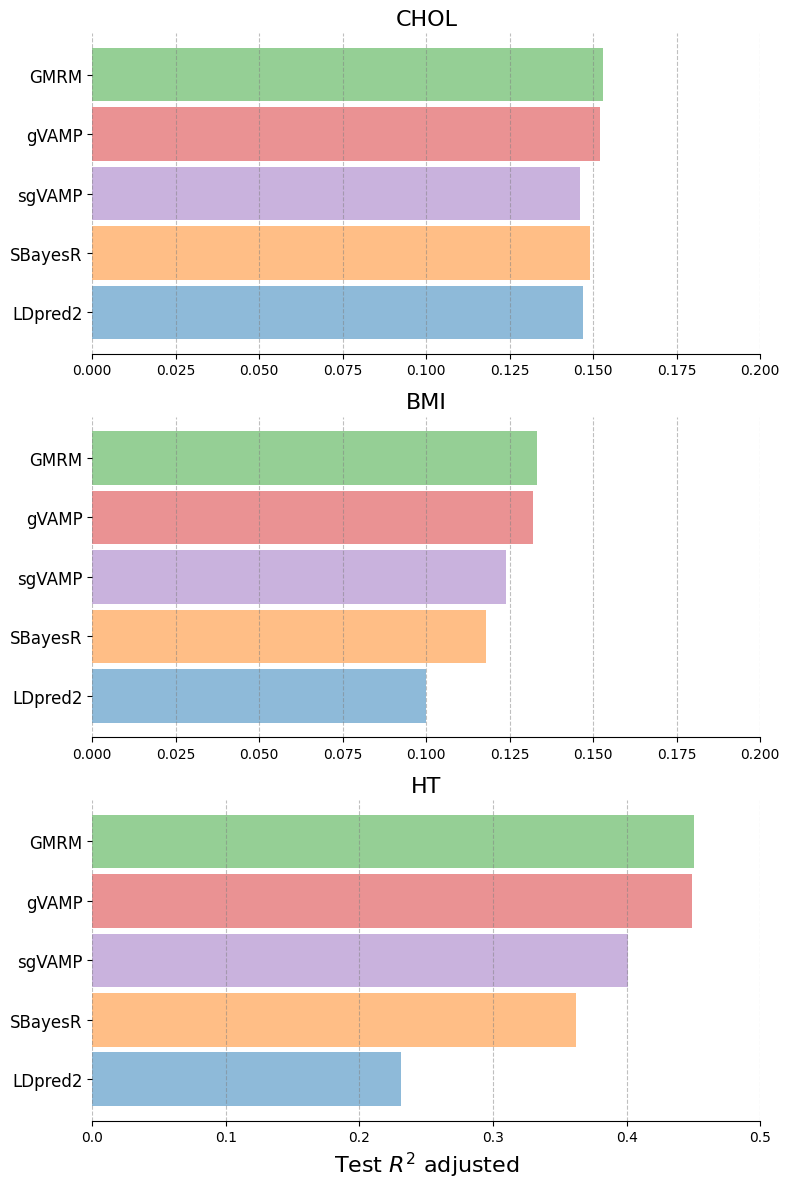
\includegraphics[width=\textwidth]{graphics/conclusion_figures/sgvamp_benchmarks.png}
        \label{fig:sgvamp_sub1}
    \end{subfigure}%
    \hfill
    \begin{subfigure}{0.45\textwidth}
        \caption{}
        \centering
        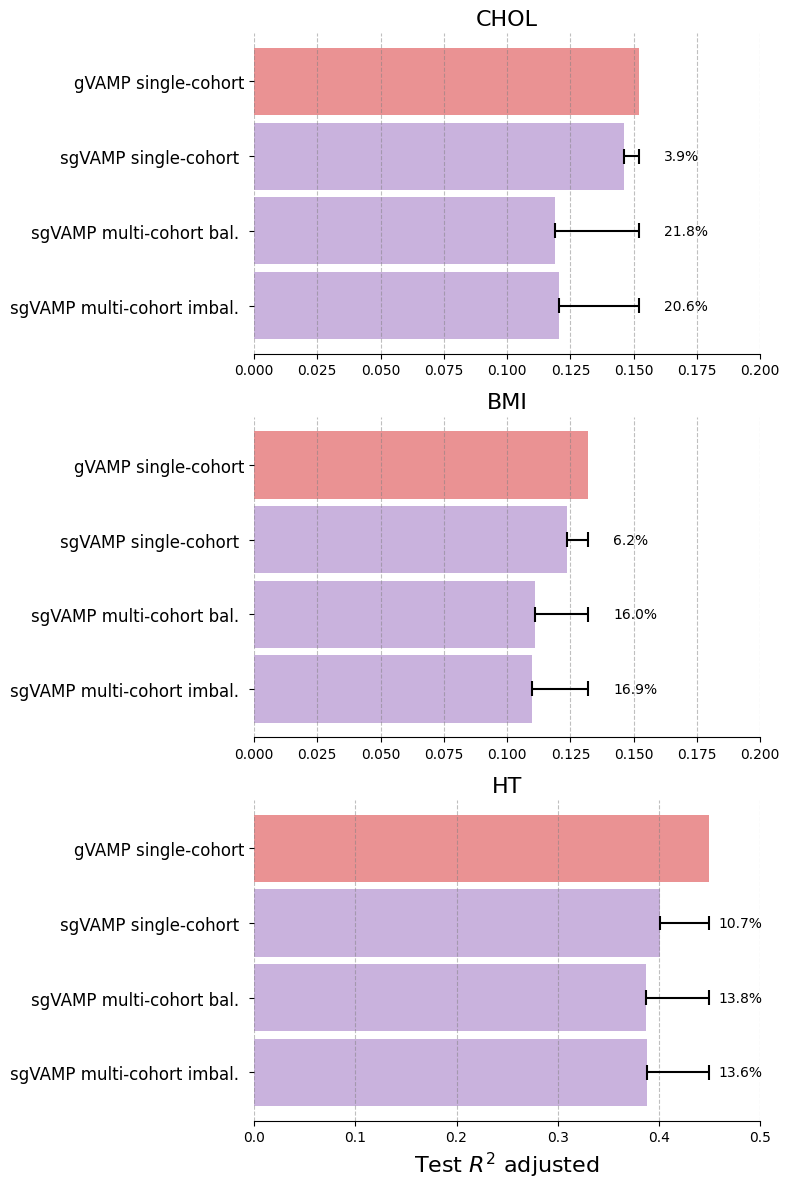
\includegraphics[width=\textwidth]{graphics/conclusion_figures/sgvamp_ukb_splits.png}
        \label{fig:sgvamp_sub2}
    \end{subfigure}
  
    \caption[Out-of-sample predictive performance of sgVAMP compared to established PRS methods and across multi-cohort splits]{\textbf{Out-of-sample predictive performance of sgVAMP compared to established PRS methods and across multi-cohort splits.} \textbf{(a)} Out-of-sample performance benchmark of sgVAMP against widely adopted polygenic risk score methods across three traits: Cholesterol (CHOL), Body Mass Index (BMI), and Standing Height (HT). The horizontal bar plots compare predictive performance (adjusted test $R^2$) across GMRM \cite{bayesrc} (green), gVAMP \cite{Depope2026} (red), sgVAMP (purple), SBayesR \cite{sbayesr} (orange), and LDpred2 \cite{ldpred} (blue). sgVAMP, the summary-level variant of gVAMP, maintains a high level of predictive accuracy, performing slightly below the individual-level state-of-the-art methods (GMRM, gVAMP) while significantly outperforming other summary-level methods for BMI and HT. The sgVAMP analysis was performed per chromosome using banded LD matrix approximations with a 1,000 kb window. Results for other methods are adapted from \cite{Depope2026}. \textbf{(b)} Predictive performance of sgVAMP in a split-cohort experiment on the UK Biobank data for CHOL, BMI, and HT. The training set was divided into either two equally sized groups (multi-cohort bal.) or two groups with a 3:1 ratio (multi-cohort imbal.). While there is an expected performance gap compared to the individual-level model trained on the full cohort, predictive accuracy remains consistent between the balanced and imbalanced data splits.}
    \label{fig:sgvamp}
\end{figure}
Figure \ref{fig:sgvamp}(a) compares the adjusted test $R^2$ performance of individual-level methods (GMRM \cite{bayesrc} and gVAMP \cite{Depope2026}) against summary-statistics methods, including our proposed summary-level version of gVAMP (sgVAMP), SBayesR \cite{sbayesr}, and LDpred2 \cite{ldpred}. Figure \ref{fig:sgvamp}(b) presents the results of a split-cohort experiment conducted on the UK Biobank dataset. We divided the training set into either two equally sized groups ("multi-cohort bal.") or two groups with a 3:1 size ratio ("multi-cohort imbal."). We evaluated the predictive performance for Cholesterol (CHOL), Body Mass Index (BMI), and Standing Height (HT) across these splits and compared it to the individual-level model trained on the full cohort. As anticipated, there is a performance gap between multi-cohort sgVAMP and the sgVAMP or gVAMP models trained on the complete dataset. Interestingly, the balanced and imbalanced split scenarios yield roughly similar predictive accuracy.

\subsection{vampW for proteomic discovery at scale}

Finally, a compelling path for future research is to apply the vampW methodology introduced in Chapter \ref{ch:vampw} to the full \gls{ukb_ppp} resource once the 600,000-sample expansion is finalized in 2027. Integrating a high-plex panel of 5,400 proteins at this scale will likely uncover substantial biological signal that remains statistically underpowered in the existing dataset. By utilizing the vampW framework, these future analyses can achieve a significant boost in discovery power while maintaining the rigorous \acrlong{fdr} control that traditional time-to-event variable selection approaches often lack.

Taking a long-term perspective, the scalability of VAMP-based inference makes it a promising candidate for the complex task of multi-omic data fusion. Integrating genomic, epigenetic, and proteomic data within a unified message-passing framework would facilitate a more holistic understanding of the regulatory networks and latent causal pathways that drive complex phenotypic traits.


\section{Conclusion}

This thesis presents novel high-dimensional statistical algorithms, built upon the Vector Approximate Message Passing framework, for joint modeling in large-scale genomics and in time-to-event proteomics data. By adopting a new perspective on inference, we move beyond the standard MCMC and variational inference techniques that form the basis of most current genome-wide association studies. A central contribution of this work is not just in the theoretical derivation of these algorithms, but in proving their practical feasibility and usefulness in large-scale computational omics. In doing so, this research bridges the gap between abstract algorithm design, scalable software implementation, and biological insights at the biobank scale.

Chapter 2 introduces gVAMP, a novel Bayesian whole-genome regression approach capable of fitting tens of millions of whole-genome sequence variants jointly for hundreds of thousands of individuals. We scale up the standard VAMP framework and combine techniques to mitigate the divergence issues commonly associated with Approximate Message Passing algorithms applied to correlated setups. Consequently, gVAMP enables joint inference at a biobank scale that far exceeds the limits of previous state-of-the-art approaches for individual-level genetic data \cite{regenie,Orliac2022}. 

By controlling for local and long-range linkage disequilibrium, it offers well-calibrated posterior inclusion probabilities that exhibit a significantly lower false discovery rate than current state-of-the-art fine-mapping methods \cite{susie,10.1093/bioinformatics/btw018}. Its capacity to handle massive whole-genome sequence inputs while providing reliable variable selection represents an important step towards a more accurate characterization of the genetic architecture of human traits. For instance, the application of gVAMP to human height data in the UK Biobank has yielded novel insights into the significant contribution of rare variation, potentially offering new avenues for prioritizing relevant genomic regions, genes, and therapeutic targets. Finally, gVAMP serves as a highly accurate tool for polygenic risk score prediction, achieving the highest reported prediction accuracy for standing human height to date. 

Chapter 3 introduces vampW, a fully parametric Bayesian survival model based on the VAMP framework for the analysis of time-to-event outcomes. We demonstrate that vampW can be applied to highly correlated proteomics data, allowing for increased prediction accuracy through the joint modeling of thousands of plasma proteins. In contrast to commonly used marginal testing and other forms of joint \acrlong{coxph}, vampW substantially reduces the false discovery rate at a similar true positive rate. The application of vampW to 24 disease outcomes in the UK Biobank study identified 219 robust protein-disease associations, many of which were missed by marginal testing. Furthermore, vampW achieves a significant improvement in the out-of-sample prediction of absolute disease onset times compared to both traditional and deep learning methods \cite{tibshirani_lasso_1997,katzman_deepsurv_2018}. These and similar future investigations have the potential to lead to a better understanding of the proteomic factors that influence when disease symptoms first appear, thereby paving the way toward personalized preventative medicine.

%%%%%%%%%%%%%%%%%%%%%%%%%%%%%%%%%%%%%%%%%%%%%%%%%%%%%%%%%%%%%%%%%%%%%%%%%%%%%%%%%%%%%%%%%%%%%%%%%%%%
%%% BACK MATTER %%%%%%%%%%%%%%%%%%%%%%%%%%%%%%%%%%%%%%%%%%%%%%%%%%%%%%%%%%%%%%%%%%%%%%%%%%%%%%%%%%%%
%%%%%%%%%%%%%%%%%%%%%%%%%%%%%%%%%%%%%%%%%%%%%%%%%%%%%%%%%%%%%%%%%%%%%%%%%%%%%%%%%%%%%%%%%%%%%%%%%%%%
\backmatter
\pagestyle{plain}

\bibliographystyle{alpha-max4} % alpha, but at most 4 authors per entry, then "et al." (alpha-max4.bst).
\renewcommand{\bibname}{References}
\bibliography{thesis, chapter_Background, chapter_gVAMP, chapter_vampW, chapter_Conclusion, intro} % Add the bibliography file (intro.bib in this case).

\mainmatter* % Remove this line to prevent numbering of appendix chapters.
\appendix % Number appendix chapters with letters instead of numbers.

\chapter{Appendix for Chapter 1}
\label{Background_Appendix}

\begin{lemma}[Bound on the Bayesian False Discovery Rate, adapted from \cite{Muller2004}]
Let $D$ be the observed GWAS data and $\mathcal{S}$ be a non-empty set of genetic variants selected as putative discoveries, with cardinality $|\mathcal{S}| > 0$. For every $j\in \mathcal{S}$, let $z_j \in \{0, 1\}$ be the unobserved, true causal indicator for variant $j$, and let $\text{PIP}_j = \mathbb{P}(z_j = 1 \mid D)$ be its \gls{pip}. Denoting the Bayesian False Discovery Rate of the set $\mathcal{S}$ as $\text{bFDR}(\mathcal{S})$, the following holds:

If there exists a constant $c \in [0, 1]$ such that $\text{PIP}_j \ge c$ for all variants $j \in \mathcal{S}$, then $\text{bFDR}(\mathcal{S}) \le 1 - c$.
\end{lemma}

\begin{proof}
The False Discovery Proportion (FDP) for the set $\mathcal{S}$ is defined as the empirical fraction of false discoveries:
\[
\text{FDP}(\mathcal{S}) = \frac{1}{|\mathcal{S}|} \sum_{j \in \mathcal{S}} (1 - z_j)
\]

The Bayesian False Discovery Rate ($\text{bFDR}$) is the posterior expectation of the FDP given the observed data $D$:
\[
\text{bFDR}(\mathcal{S}) = \mathbb{E}[\text{FDP}(\mathcal{S}) \mid D] = \mathbb{E} \left[ \frac{1}{|\mathcal{S}|} \sum_{j \in \mathcal{S}} (1 - z_j) \biggm| D \right]
\]

By the linearity of the expectation operator, we can move the expectation inside the summation. Furthermore, because $z_j$ is a Bernoulli random variable (taking values $0$ or $1$), its expected value is equal to its probability of being equal to $1$:
\[
\mathbb{E}[z_j \mid D] = P(z_j = 1 \mid D) = \text{PIP}_j
\]

Substituting this into the $\text{bFDR}$ equation yields:
\begin{align*}
\text{bFDR}(\mathcal{S}) &= \frac{1}{|\mathcal{S}|} \sum_{j \in \mathcal{S}} \mathbb{E}[(1 - z_j) \mid D] \\
&= \frac{1}{|\mathcal{S}|} \sum_{j \in \mathcal{S}} (1 - \mathbb{E}[z_j \mid D]) \\
&= \frac{1}{|\mathcal{S}|} \sum_{j \in \mathcal{S}} (1 - \text{PIP}_j)
\end{align*}

% -\text{PIP}_j &\le -c \\
Assume the premise of the lemma: for all $j \in \mathcal{S}$, $\text{PIP}_j \ge c$. It follows that:
\begin{align*}
1 - \text{PIP}_j &\le 1 - c
\end{align*}

We substitute this inequality into the simplified $\text{bFDR}$ equation:
\[
\text{bFDR}(\mathcal{S}) \le \frac{1}{|\mathcal{S}|} \sum_{j \in \mathcal{S}} (1 - c)
\]

Since $(1 - c)$ is a constant with respect to the summation index $j$, summing it $|\mathcal{S}|$ times yields:
\begin{align*}
% \text{bFDR}(\mathcal{S}) &\le \frac{1}{|\mathcal{S}|} \times |\mathcal{S}| \times (1 - c) \\
\text{bFDR}(\mathcal{S}) &\le 1 - c
\end{align*}
\end{proof}

\newpage

\begin{breakablealgorithm}{Expectation-Maximization Vector Approximate Message Passing for Generalized Linear Models}{Expectation-Maximization Vector Approximate Message Passing for Generalized Linear Models \cite{schniter_vector_2016,emGVAMP2018}.}{EMVAMP-GLM}
    \begin{algorithmic}[1]
        \STATE {\bfseries Input:} design matrix $\bm{X} \in \mathbb{R}^{N \times P}$, observed vector of outcomes $\mathbf{y} \in \mathbb{R}^N$, number of iterations $N_{\text{it}}$, initial estimate of effect sizes $\bm{r}_{1,0} \in \mathbb{R}^P$, initial effect size precision $\gamma_{1,0} \ge 0$, initial estimate of linear predictor $\bm{p}_{1,0} \in \mathbb{R}^N$, initial linear predictor precision $\tau_{1,0} \ge 0$, initial prior parameters $\Theta_{0}$ belonging to a space of prior parameters $\bm{\Theta}$, initial observation model parameters $\Phi_{0}$ belonging to a space of model parameters $\bm{\Phi}$, and denoisers $g_1 : \mathbb{R} \times \mathbb{R} \times \bm{\Theta} \to \mathbb{R}$ and $g_2 : \mathbb{R} \times \mathbb{R} \times \mathbb{R} \times \bm{\Phi} \to \mathbb{R}$ satisfying: $g_1$ and $g_2$ are separable with identical Lipschitz components applied elementwise, i.e., $[g_1(\bm{r}, \gamma, \Theta)]_n = g_1(r_n, \gamma, \Theta)$ $\forall n$ and $[g_2(\bm{p}, \tau, \mathbf{y}, \Phi)]_n = g_2(p_n, y_n, \tau, \Phi)$ $\forall n$.
        \FOR{$t = 0, 1,\dots, N_{\text{it}}$}

            \STATE {\bfseries Prior denoising step}
            \STATE EM update of the prior distribution parameters $\Theta \in \bm{\Theta}$, called $\Theta_t$
            \STATE $\hat{\bm{\beta}}_{1,t} = g_{1}(\bm{r}_{1,t}, \gamma_{1,t}, \Theta_t)$
            \STATE $\alpha_{1,t} = \gamma_{1,t} \cdot \langle g_{1}'(\bm{r}_{1,t}, \gamma_{1,t}, \Theta_t) \rangle$
            \STATE $\gamma_{2,t} = \gamma_{1,t} \cdot (1 - \alpha_{1,t}) / \alpha_{1,t}$
            \STATE $\bm{r}_{2,t} = (\hat{\bm{\beta}}_{1,t} - \alpha_{1,t} \bm{r}_{1,t}) / (1-\alpha_{1,t})$
            \item[]

            \STATE {\bfseries Observation model denoising step}
            \STATE EM update of the observation model parameters $\Phi \in \bm{\Phi}$, called $\Phi_t$
            \STATE $\hat{\bm{z}}_{1,t} = g_{2}(\bm{p}_{1,t}, \tau_{1,t}, \mathbf{y}, \Phi_t)$
            \STATE $\upsilon_{1,t} = \tau_{1,t} \cdot \langle g_{2}'(\bm{p}_{1,t}, \tau_{1,t}, \mathbf{y}, \Phi_t) \rangle$
            \STATE $\tau_{2,t} = \tau_{1,t} \cdot (1 - \upsilon_{1,t}) / \upsilon_{1,t}$
            \STATE $\bm{p}_{2,t} = (\hat{\bm{z}}_{1,t} - \upsilon_{1,t} \bm{p}_{1,t}) / (1-\upsilon_{1,t})$
            \item[]

            \STATE {\bfseries LMMSE step for $\bm{\beta}$}
            \STATE $\hat{\bm{\beta}}_{2,t} = ( \tau_{2,t} \bm{X}^\top\bm{X} + \gamma_{2,t} \bm{I} )^{-1} ( \tau_{2,t} \bm{X}^\top \bm{p}_{2,t} + \gamma_{2,t} \bm{r}_{2,t} )$
            \STATE $\alpha_{2,t} = \gamma_{2,t} \cdot \mathrm{Tr}[(\tau_{2,t} \bm{X}^\top\bm{X} + \gamma_{2,t}\bm{I})^{-1}] / P$
            \STATE $\gamma_{1,t+1} = \gamma_{2,t} \cdot (1-\alpha_{2,t}) / \alpha_{2,t}$
            \STATE $\bm{r}_{1,t+1} = (\hat{\bm{\beta}}_{2,t} - \alpha_{2,t} \bm{r}_{2,t}) / (1-\alpha_{2,t})$
            \item[]

            \STATE {\bfseries LMMSE step for $\bm{z} = \bm{X}\bm{\beta}$}
            \STATE $\hat{\bm{z}}_{2,t} = \bm{X} \hat{\bm{\beta}}_{2,t}$
            \STATE $\upsilon_{2,t} = \tau_{2,t} \cdot \mathrm{Tr}[\bm{X}(\tau_{2,t} \bm{X}^\top\bm{X} + \gamma_{2,t}\bm{I})^{-1}\bm{X}^\top] / N$
            \STATE $\tau_{1,t+1} = \tau_{2,t} \cdot (1-\upsilon_{2,t}) / \upsilon_{2,t}$
            \STATE $\bm{p}_{1,t+1} = (\hat{\bm{z}}_{2,t} - \upsilon_{2,t} \bm{p}_{2,t}) / (1-\upsilon_{2,t})$

        \ENDFOR
        \STATE \textbf{return} $\hat{\bm{\beta}}_{1,t}$
    \end{algorithmic}
\end{breakablealgorithm}

The prior denoising function is often chosen to minimize mean squared error: $g_{1}(\bm{r}, \gamma, \Theta) = \mathbb{E}[\bm{\beta} \mid \bm{r} = \bm{\beta} + \mathcal{N}(0, \gamma^{-1}\bm{I}), \gamma, \Theta]$ with derivative $g_{1}'(\bm{r}, \gamma, \Theta) = \gamma \cdot \mathrm{Var}[\bm{\beta} \mid \bm{r} = \bm{\beta} + \mathcal{N}(0, \gamma^{-1}\bm{I}), \gamma, \Theta]$. The observation model denoising function is analogously often used with $g_{2}(\bm{p}, \tau, \mathbf{y}, \Phi) = \mathbb{E}[\bm{z} \mid \bm{p} = \bm{z} + \mathcal{N}(0, \tau^{-1}\bm{I}), \mathbf{y}, \tau, \Phi]$ and derivative $g_{2}'(\bm{p}, \tau, \mathbf{y}, \Phi) =  \tau \cdot \mathrm{Var}[\bm{z} \mid \bm{p} = \bm{z} + \mathcal{N}(0, \tau^{-1}\bm{I}), \mathbf{y}, \tau, \Phi]$.


\chapter{Appendix for Chapter 2}

\section{Supplementary tables}

\begin{table}[!htp]
\caption[Simulation settings using whole genome sequence (WGS) data of chromosomes 11 to 15 in the UK Biobank]{\textbf{Simulation settings using whole genome sequence (WGS) data of chromosomes 11 to 15 in the UK Biobank.} \small{Each setting varies in the number of causal variants (CV), the frequency-based enrichment parameter ($\gamma$), and the effect-size–MAF relationship ($\alpha$, see Methods for the description of the parameters). All scenarios shown use $h^2 = 7.25\%$.}}
\begin{center}
\begin{tabular}{|| c | c | c | c ||} 
 \hline
ID & Number of causal variants & $\gamma$ & $\alpha$ \\ [0.5ex] 
 \hline\hline
a & 500 & 0 & -1 \\
\hline
b & 500 & 50 & -1 \\
\hline
c & 1000 & 0 & -1 \\
\hline
d & 1000 & 50 & -1 \\
\hline
e & 500 & 0 & -0.5 \\
\hline
f & 500 & 50 & -0.5 \\
\hline
g & 1000 & 0 & -0.5 \\
\hline
h & 1000 & 50 & -0.5 \\
\hline
i & 500 & 0 & -0.25 \\
\hline
j & 500 & 50 & -0.25 \\
\hline
k & 1000 & 0 & -0.25 \\
\hline
l & 1000 & 50 & -0.25 \\
\hline\hline
\end{tabular}
\end{center}
\label{table:S1}
\end{table}


\newpage

\begin{table}[!htp]
\caption[The $13$ UK Biobank traits used within the study]{\textbf{The $13$ UK Biobank traits used within the study}. \small Phenotypic names and their
codes used in the study. The sample size, $N$, gives the number of individuals with training data measures.}
\begin{center}
\begin{tabular}{|| c | c | c ||} 
 \hline
Phenotype & Code & Sample size, $N$ \\ [0.5ex] 
 \hline\hline
Blood: cholesterol & CHOL & 395,025  \\
 \hline 
Blood: eosinophill count & EOSI & 401,452  \\
 \hline 
Blood: glycated haemoglobin & HbA1c & 394,912  \\
 \hline
Blood: High density lipoprotein & HDL & 360,286  \\
 \hline
Blood: mean corpuscular haemoglobin & MCH & 402,201  \\
 \hline
Blood mean corpuscular volume & MCV & 402,202  \\
 \hline
Red blood cell count & RBC & 402,204  \\
 \hline
Body mass index & BMI & 413,595  \\
 \hline
Diastolic blood pressure & DBP & 377,358   \\
 \hline
Forced vital capacity & FVC & 376,724  \\
 \hline 
Heel bone mineral density & BMD & 231,693  \\
 \hline
Standing height  & HT & 414,055   \\
 \hline
Systolic blood pressure & SBP & 377,347  \\
\hline\hline
\end{tabular}
%}
\end{center}
\label{table:tableS2}
\end{table}

\newpage


\begin{table}[!htp]
\caption[Genome-wide significant associations for $13$ UK Biobank traits from the software gVAMP and LDAK-KVIK at 8,430,446 genetic variants from mixed linear model association leave-one-chromosome-out (MLMA-LOCO) testing]{\textbf{Genome-wide significant associations for $13$ UK Biobank traits from the software gVAMP and LDAK-KVIK at 8,430,446 genetic variants from mixed linear model association leave-one-chromosome-out (MLMA-LOCO) testing.} \small{"LDAK 2M LOCO" refers to MLMA-LOCO testing at 8,430,446 SNPs, using the LDAK-KVIK software in step 1, with 2,174,071 SNP markers. "gVAMP 2M LOCO 1" refers to MLMA-LOCO testing at 8,430,446 SNPs, using the framework presented here, where in step 1 2,174,071 markers are used and the second step is identical to that of LDAK-KVIK. "gVAMP 2M LOCO 2" is the same as "gVAMP 2M LOCO 1" but with the second step identical to REGENIE. The values are the number of genome-wide significant linkage disequilibrium independent associations selected based upon a standard $p$-value threshold of less than $5 \cdot 10^{-8}$ and $R^2$ between SNPs in a 1 Mb genomic segment of less than $1\%$.}}
\begin{center}
\resizebox{0.6\columnwidth}{!}{%
\begin{tabular}{|| c || c || c | c | c || c ||} 
 \hline
Trait & LDAK & gVAMP & gVAMP \\ [0.25ex]
 & 2M LOCO & 2M LOCO & 2M LOCO \\ [0.25ex]
  & & 1 & 2 \\ [0.25ex]
 \hline\hline
CHOL & 482 & 625 & 603  \\
 \hline 
EOSI &  549 & 666 & 630  \\
 \hline 
HbA1c &  321 & 400 & 385  \\
 \hline
HDL & 639 & 855 & 812  \\
 \hline
MCH & 690 & 858 & 810  \\
 \hline
MCV & 903 & 1128 & 1062  \\
 \hline
RBC & 856 & 1140 & 1079  \\
 \hline
BMI & 726 & 1202 & 1175\\
 \hline
DBP & 303 & 357 & 419  \\
 \hline
FVC & 577 & 759 & 721 \\
 \hline 
BMD & 549 & 681 & 668 \\
 \hline
HT & 2703 & 4747 & 4452 \\
 \hline
SBP & 323 & 410 & 388 \\
\hline\hline
\end{tabular}
}
\end{center}
\label{table:tableS3}
\end{table}

\newpage

\section{Supplementary figures}

\begin{figure}[!htp]
    \centering
    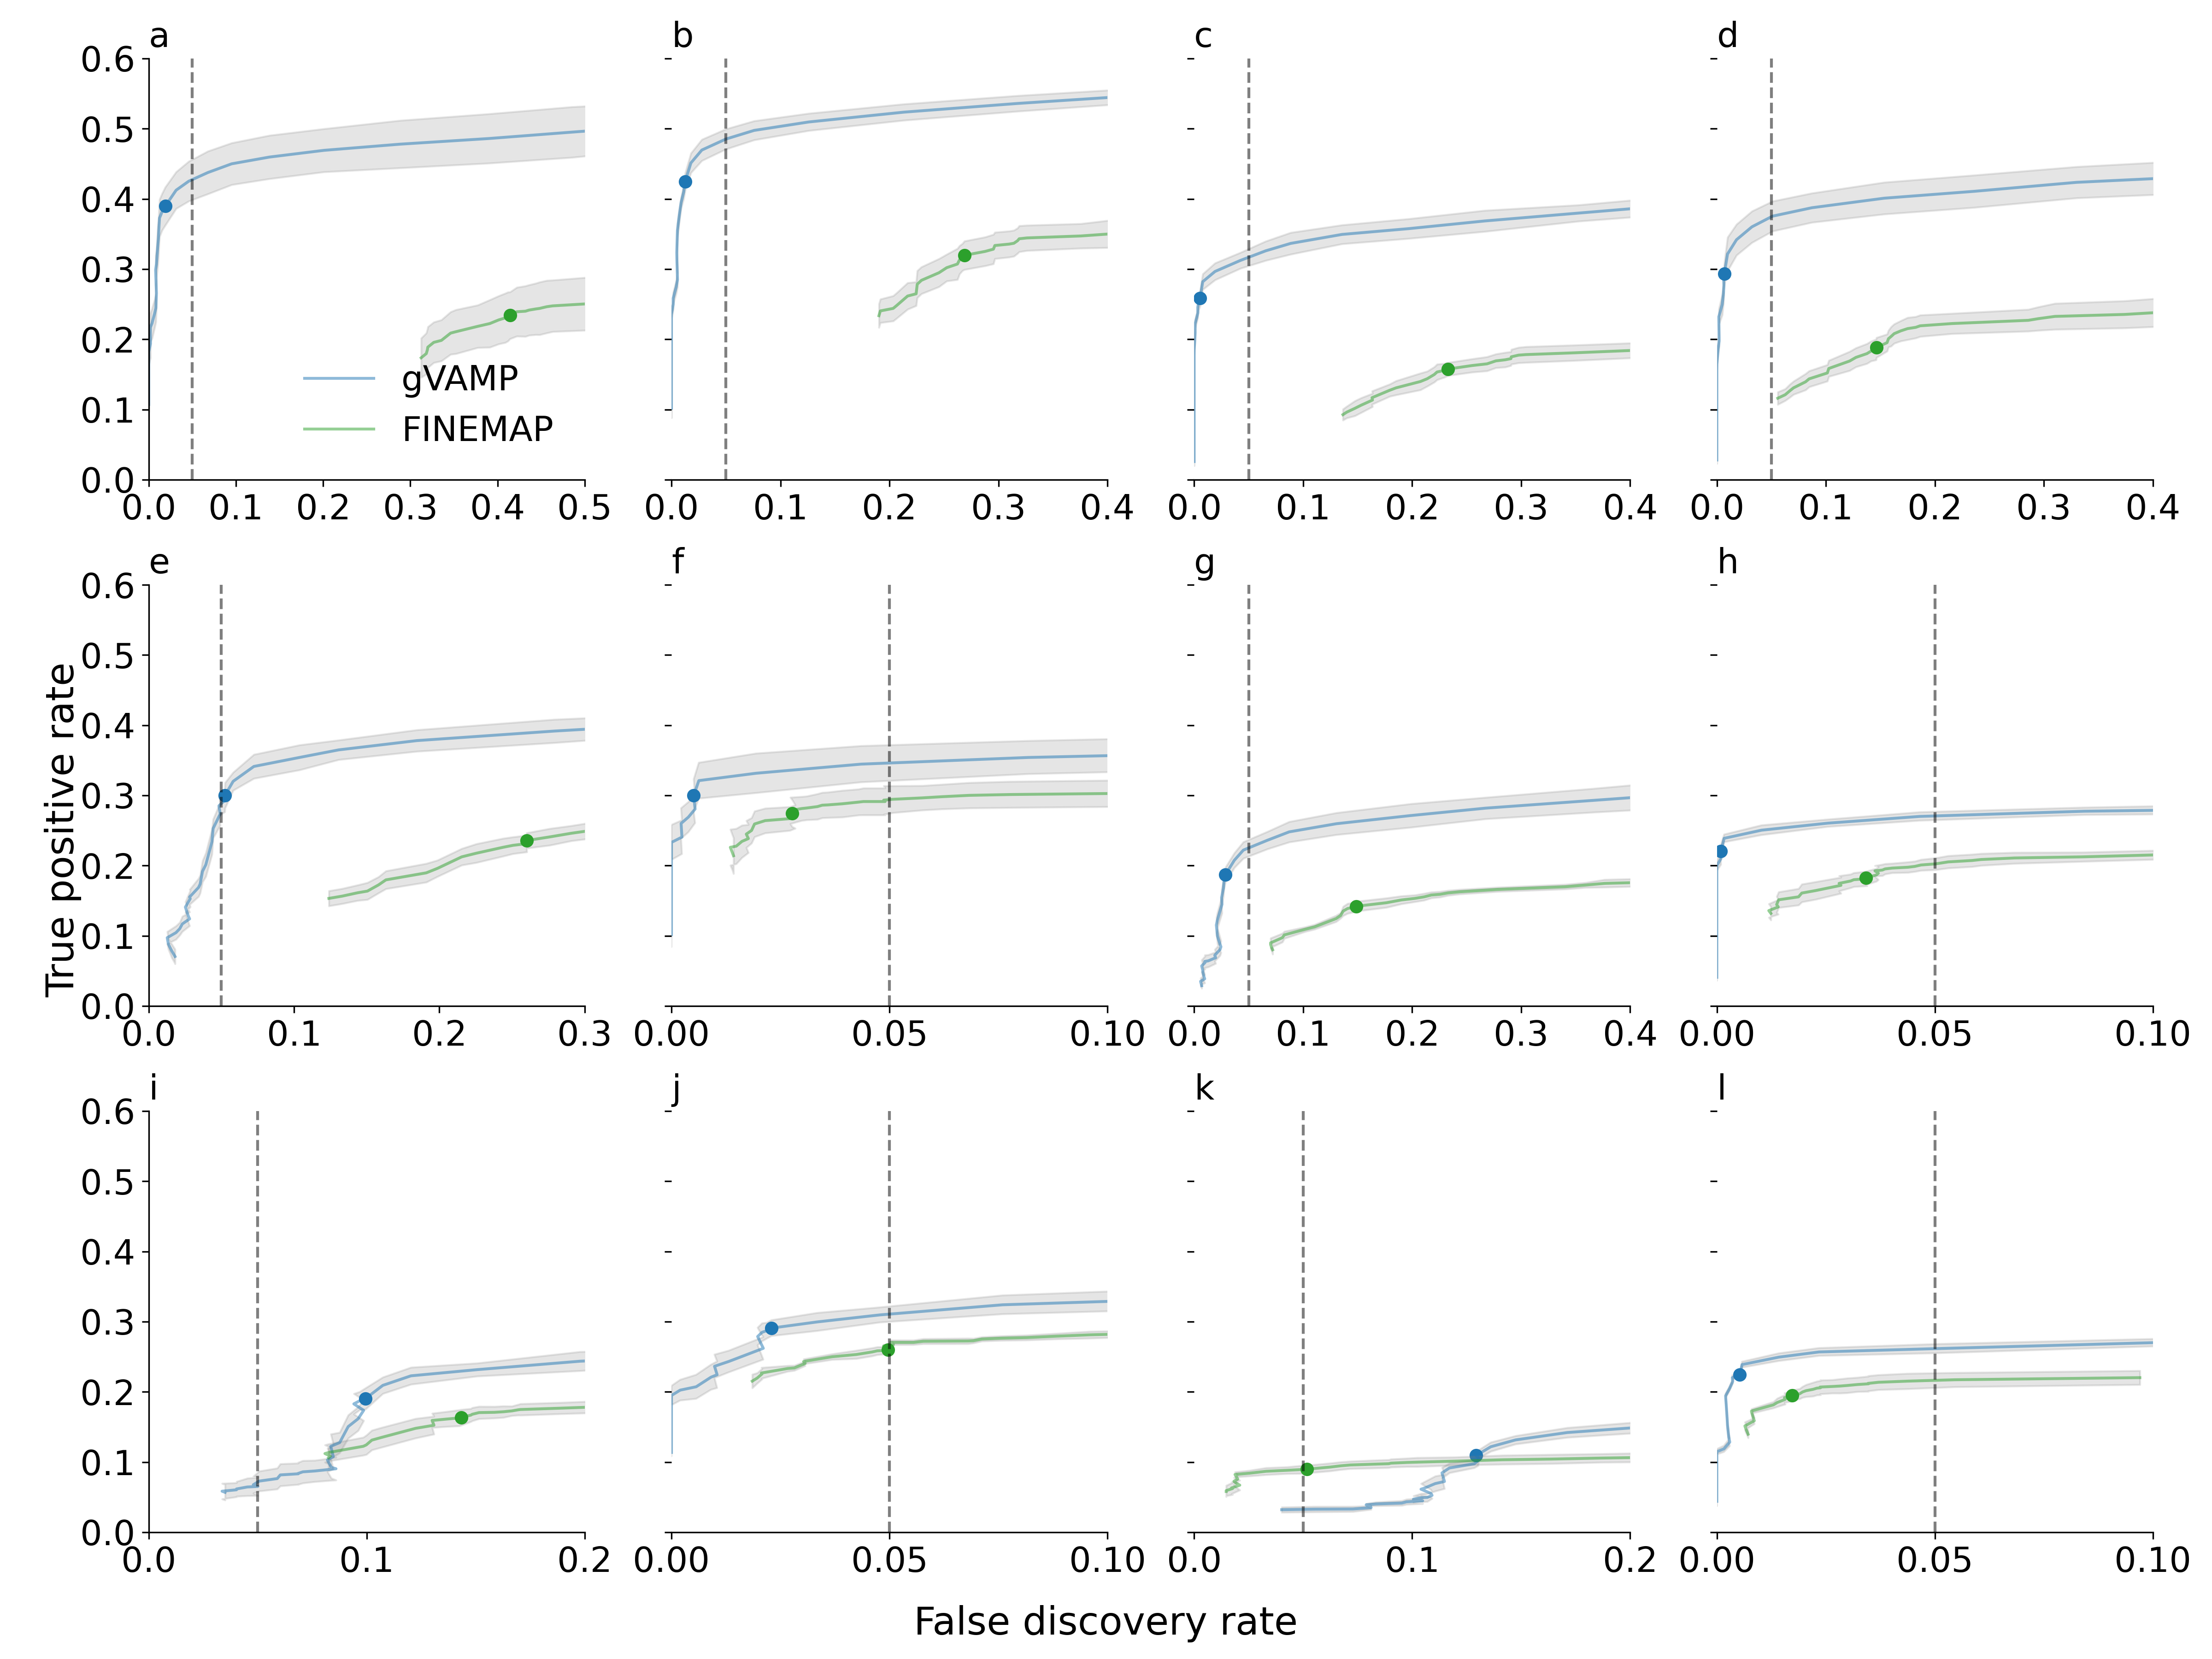
\includegraphics[width=\linewidth]{graphics/gVAMP_figures/v4/FigS1.png}
    \caption[Comparison of the true positive rate (TPR, $y$-axis) versus the false discovery rate (FDR, $x$-axis) between gVAMP and marginal GWAS association testing plus fine-mapping implemented in the FINEMAP algorithm across 12 simulation scenarios using whole genome sequence (WGS) data of chromosomes 11 to 15 in the UK Biobank]{\textbf{Comparison of the true positive rate (TPR, $y$-axis) versus the false discovery rate (FDR, $x$-axis) between gVAMP and marginal GWAS association testing plus fine-mapping implemented in the FINEMAP algorithm across 12 simulation scenarios using whole genome sequence (WGS) data of chromosomes 11 to 15 in the UK Biobank.} \small For the detailed description of different simulation settings, see Methods and Supplementary Table \ref{table:S1}. We use a Bonferroni corrected p-value significance threshold for marginal GWAS testing and then having identified associated regions we examine the ability of FINEMAP (green) to conduct variable selection across posterior inclusion probability (PIP) thresholds. For gVAMP (blue), variable selection is conducted from PIP values obtained from a single model run genome-wide. Error bands give the standard deviation across 5 simulation replicates. The blue and green dots give the TPR and FDR at PIP $\geq 0.95$, which should correspond to an FDR of $\leq 0.05$ if the model correctly conducts variable selection based on PIP values.}
    \label{fig:finalFigS1}
\end{figure}

\newpage

\begin{figure}[!htp]
    \centering
    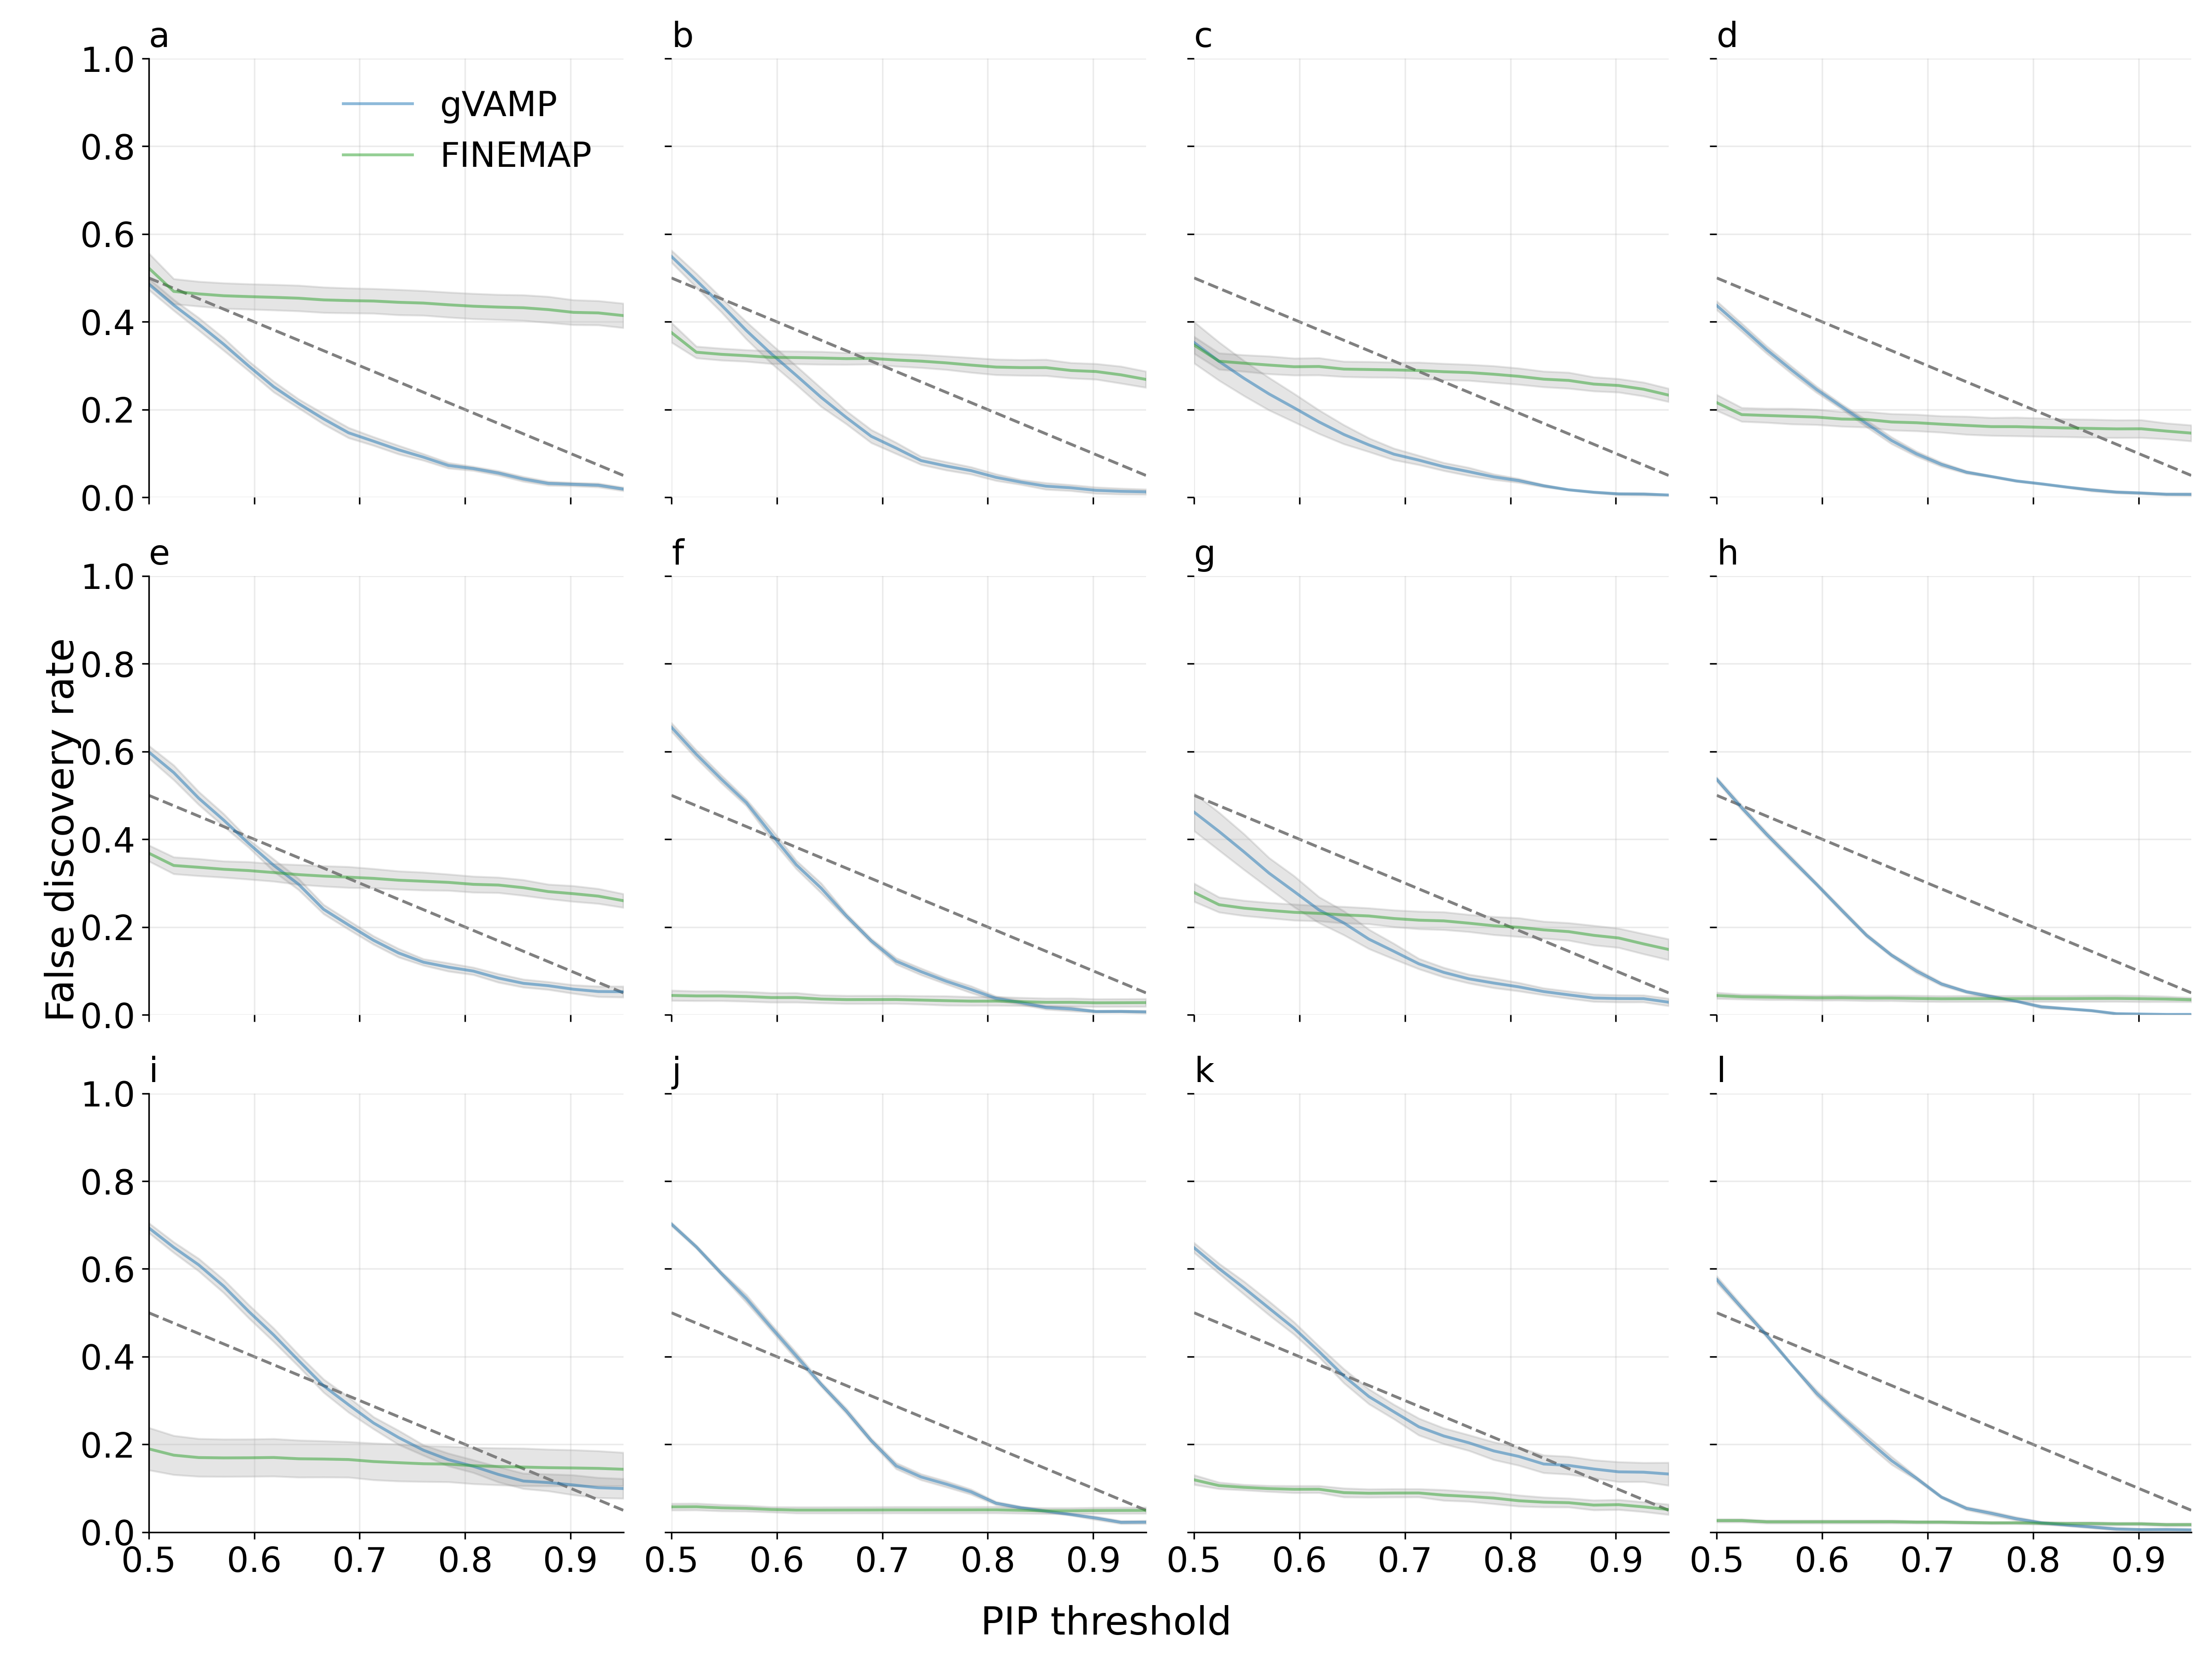
\includegraphics[width=\linewidth]{graphics/gVAMP_figures/v4/FigS2.png}
    \caption[Comparison of the posterior inclusion probability threshold (PIP threshold, $x$-axis) versus the false discovery rate (FDR, $y$-axis) between gVAMP and marginal GWAS association testing plus fine-mapping implemented in the FINEMAP algorithm across 12 simulation scenarios using whole genome sequence data of chromosomes 11 to 15 in the UK Biobank]{\textbf{Comparison of the posterior inclusion probability threshold (PIP threshold, $x$-axis) versus the false discovery rate (FDR, $y$-axis) between gVAMP and marginal GWAS association testing plus fine-mapping implemented in the FINEMAP algorithm across 12 simulation scenarios using whole genome sequence (WGS) data of chromosomes 11 to 15 in the UK Biobank.} \small For the detailed description of different simulation settings, see Methods and Supplementary Table \ref{table:S1}. We use a Bonferroni corrected p-value significance threshold for marginal GWAS testing and then having identified associated regions we examine the ability of FINEMAP (green) to conduct variable selection across PIP thresholds. For gVAMP (blue), variable selection is conducted from PIP values obtained from a single model run genome-wide. Error bands give the standard deviation across 5 simulation replicates. Dashed lines gives the maximum FDR expected at different PIP thresholds for a model that correctly conducts variable selection based on PIP values.}
    \label{fig:finalFigS2}
\end{figure}

\newpage

\begin{figure}[!htp]
    \centering
    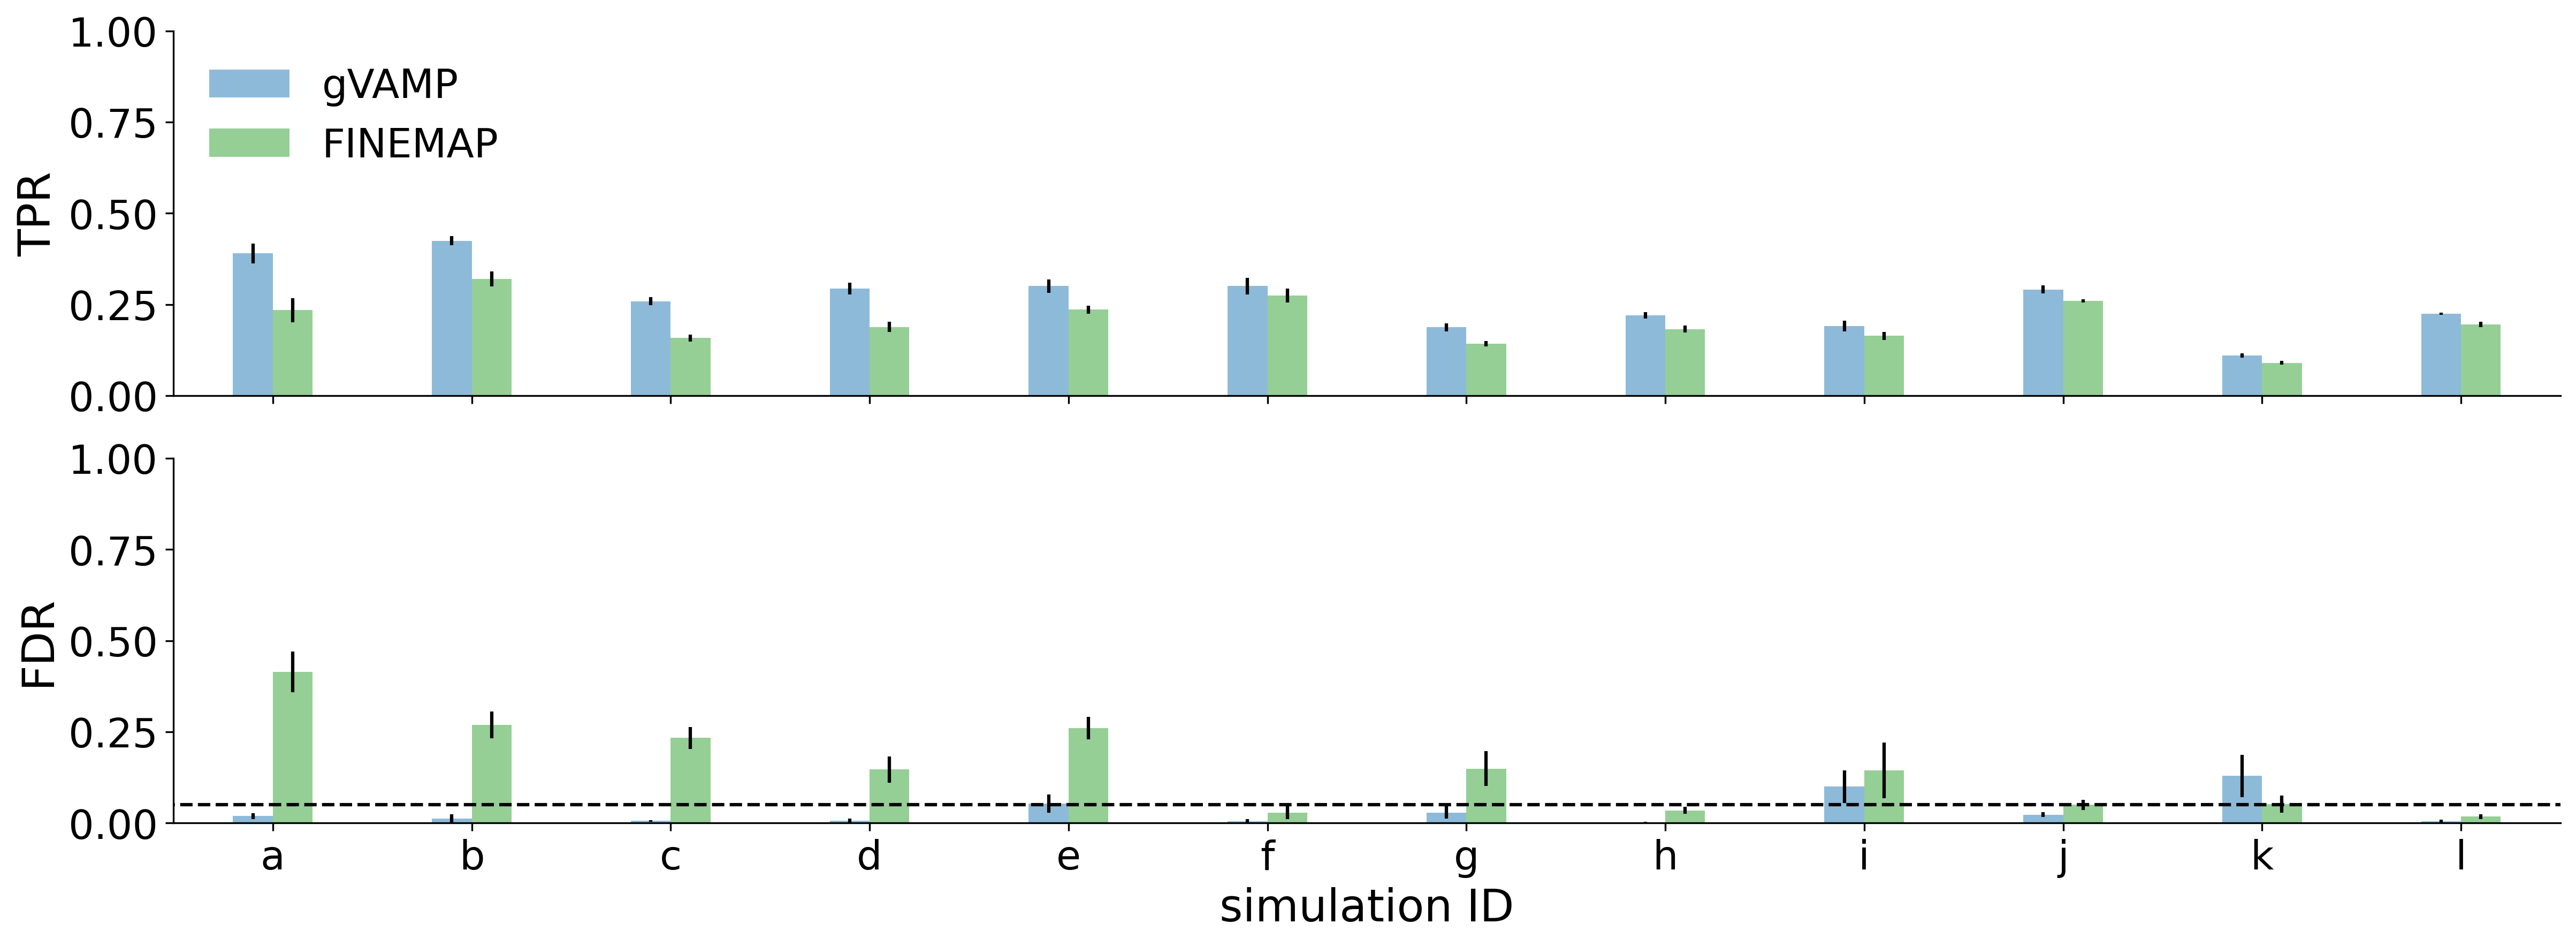
\includegraphics[width=\linewidth]{graphics/gVAMP_figures/v4/FigS3.png}
    \caption[Performance in terms of the true positive rate (TPR) and the false discovery rate (FDR) of marginal GWAS testing plus fine-mapping with FINEMAP, and gVAMP at posterior inclusion probability $\ge 0.95$ in a whole genome sequence data simulation study of chromosomes 11 to 15 in the UK Biobank]{\textbf{Performance in terms of the true positive rate (TPR) and the false discovery rate (FDR) of marginal GWAS testing plus fine-mapping with FINEMAP, and gVAMP at posterior inclusion probability $\ge 0.95$ in a whole genome sequence (WGS) data simulation study of chromosomes 11 to 15 in the UK Biobank.} \small We use a Bonferroni corrected p-value significance threshold for marginal GWAS and PIP $>0.95$ for FINEMAP (green) applied for regions identified as significant in the marginal analysis. FINEMAP controls the FDR in only 5 out of 12 WGS data simulation settings (see Methods and Supplementary Table \ref{table:S1}). In contrast, using a PIP $>0.95$ threshold for the gVAMP testing (blue) controls FDR in 10 out of 12 settings, whilst yielding consistently higher TPR across all settings. Error bars give the standard deviation across 5 simulation replicates.}
    \label{fig:finalFigS3}
\end{figure}

\newpage

\begin{figure}[!htp]
    \centering
    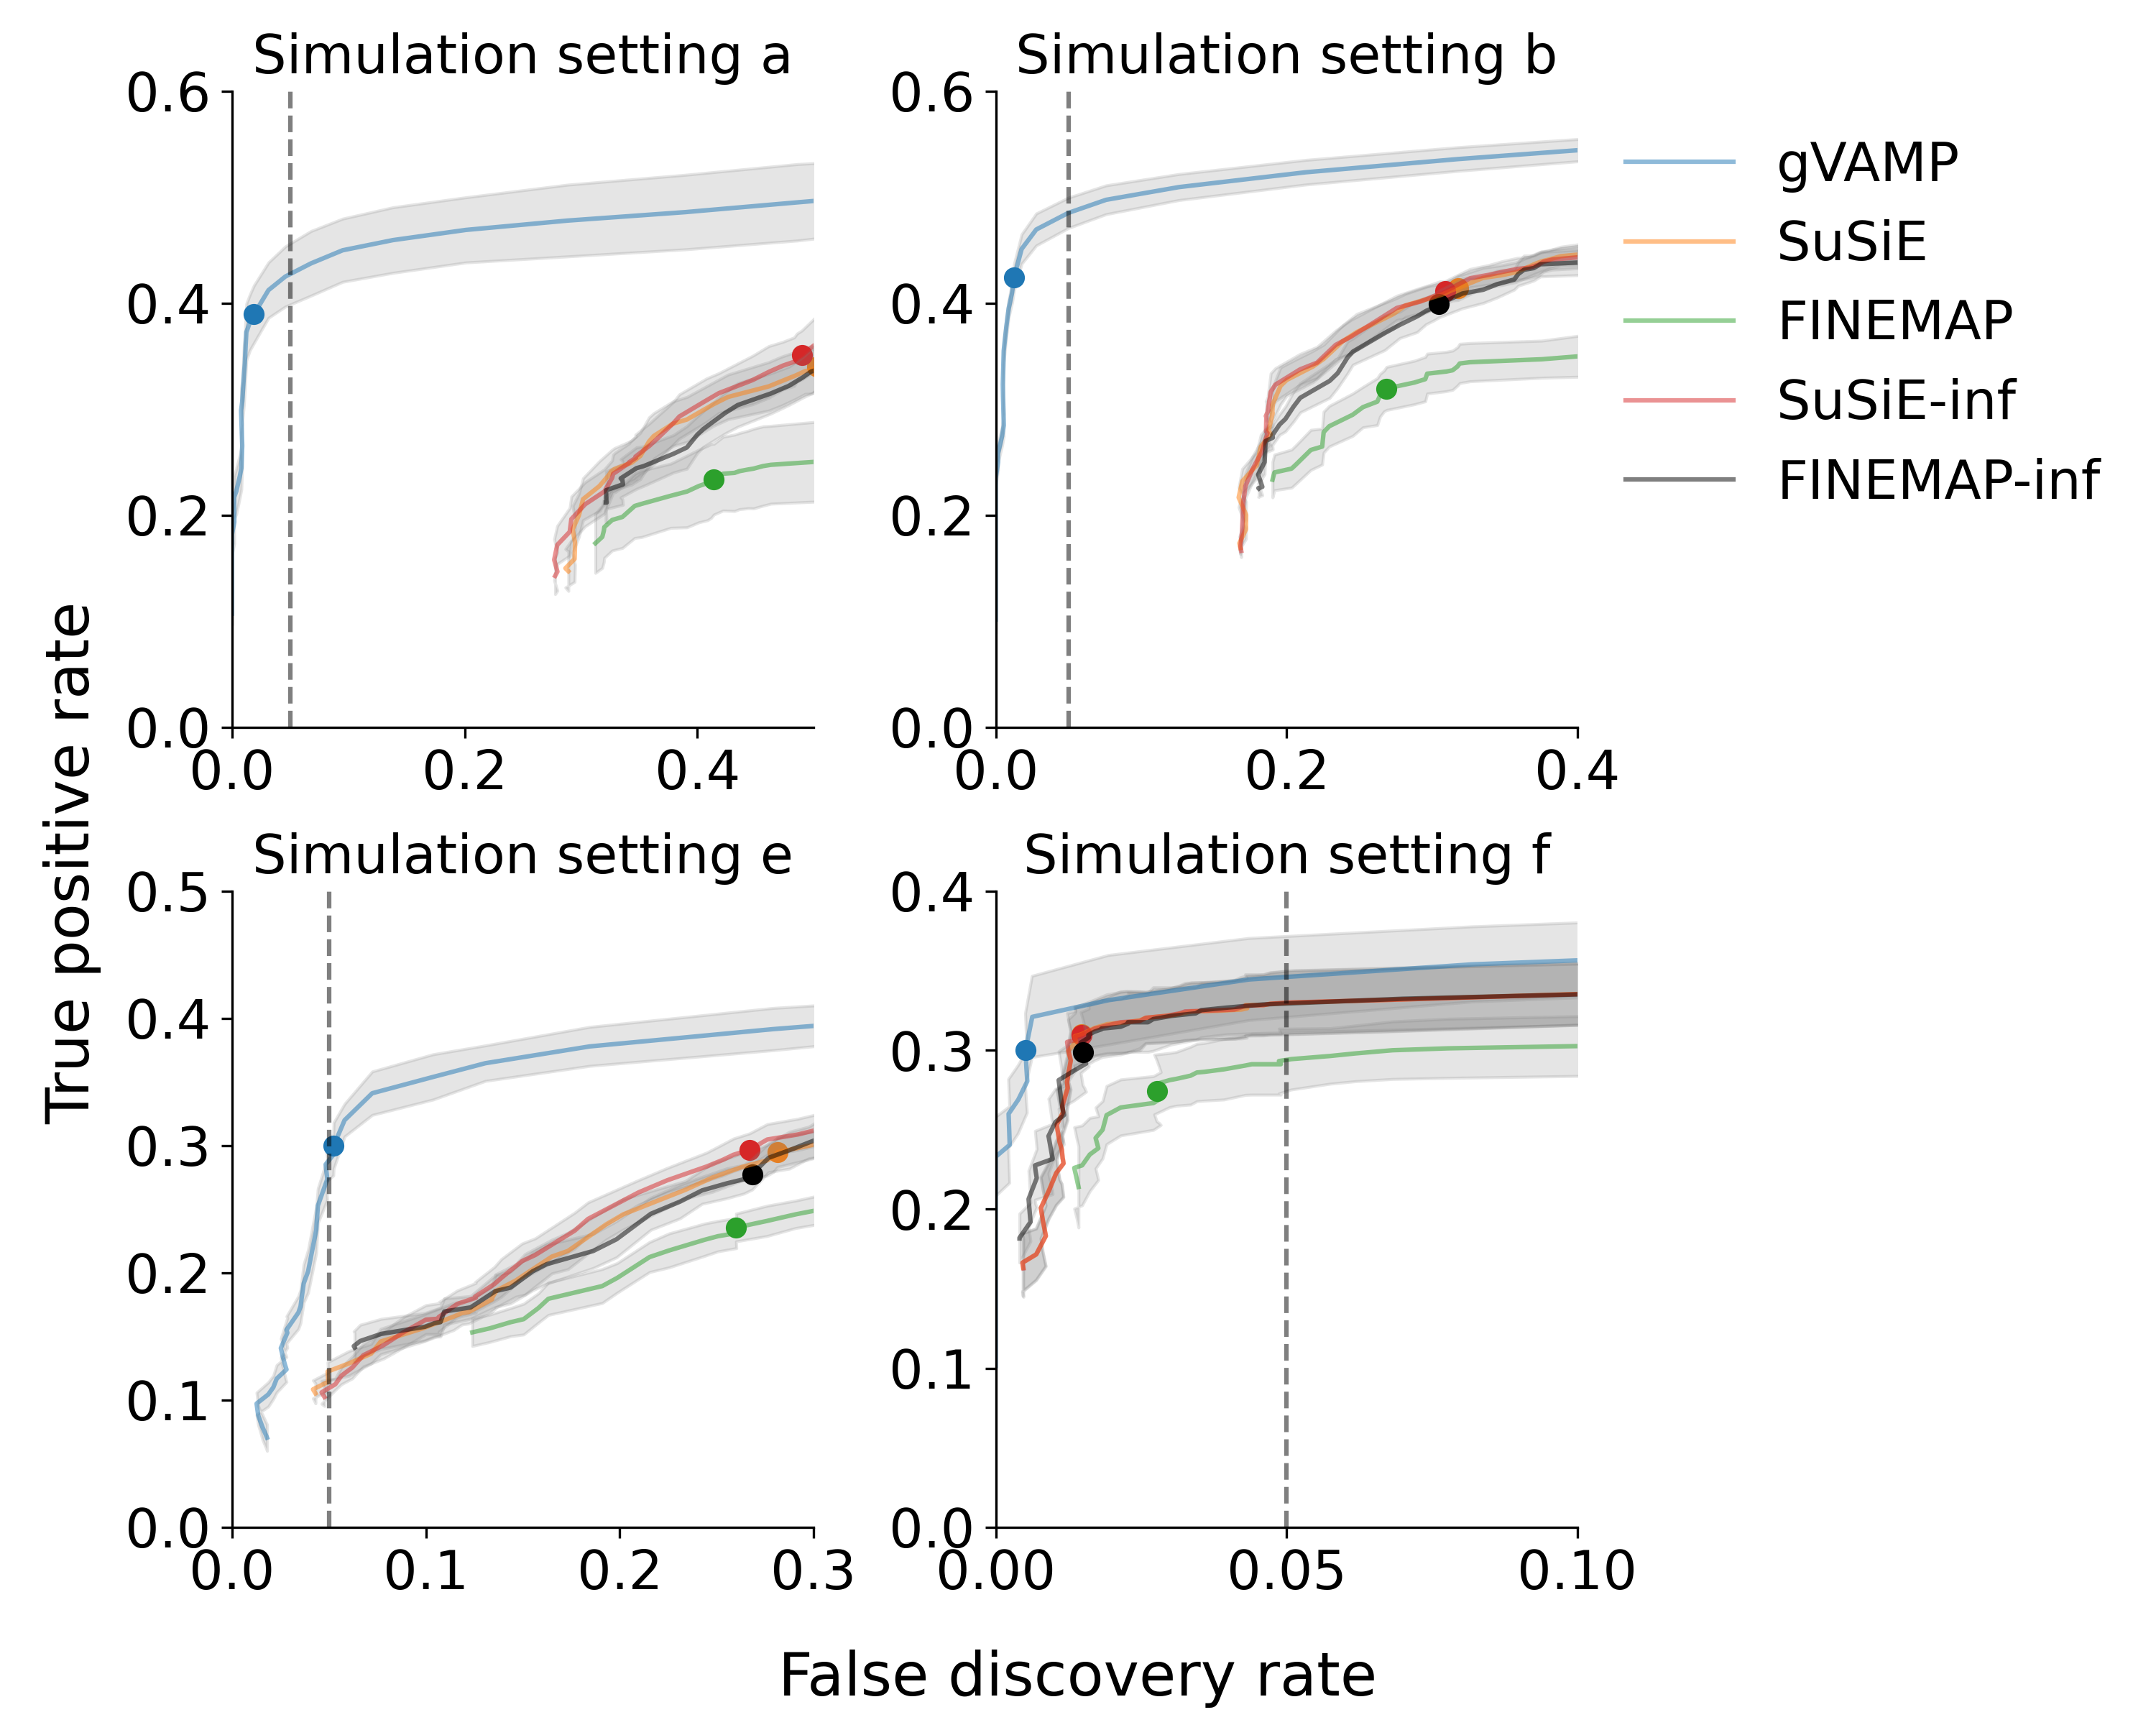
\includegraphics[width=\linewidth]{graphics/gVAMP_figures/v4/FigS4.png}
    \caption[Benchmarking of gVAMP to a wide range of fine-mapping methods applied to marginal GWAS summary data in a whole genome sequence data simulation study of chromosomes 11 to 15 in the UK Biobank]{\textbf{Benchmarking of gVAMP to a wide range of fine-mapping methods applied to marginal GWAS summary data in a whole genome sequence (WGS) data simulation study of chromosomes 11 to 15 in the UK Biobank.} \small For the detailed description of different simulation settings, see Methods and Supplementary Table \ref{table:S1}. We use a Bonferroni corrected p-value significance threshold for marginal GWAS testing and then having identified associated regions we apply FINEMAP (green) and SuSiE (orange) to conduct variable selection across PIP thresholds. We also compare to SuSiE-inf (red) and FINEMAP-inf (black) run genome-wide. We compare the true positive rate (TPR) and false discovery rate (FDR) of the methods, with coloured dots indicating the TPR and FDR at $\geq 0.95$ PIP, lines giving the TPR and FDR across PIP thresholds and error bands giving the standard deviation across 5 simulation replicates. SuSiE-inf and FINEMAP-inf improve the TPR, but generally not the FDR. gVAMP gives consistently higher TPR at FDR $\leq 5\%$.}
    \label{fig:finalFigS7}
\end{figure}

\newpage

\begin{figure}[!htp]
    \centering
    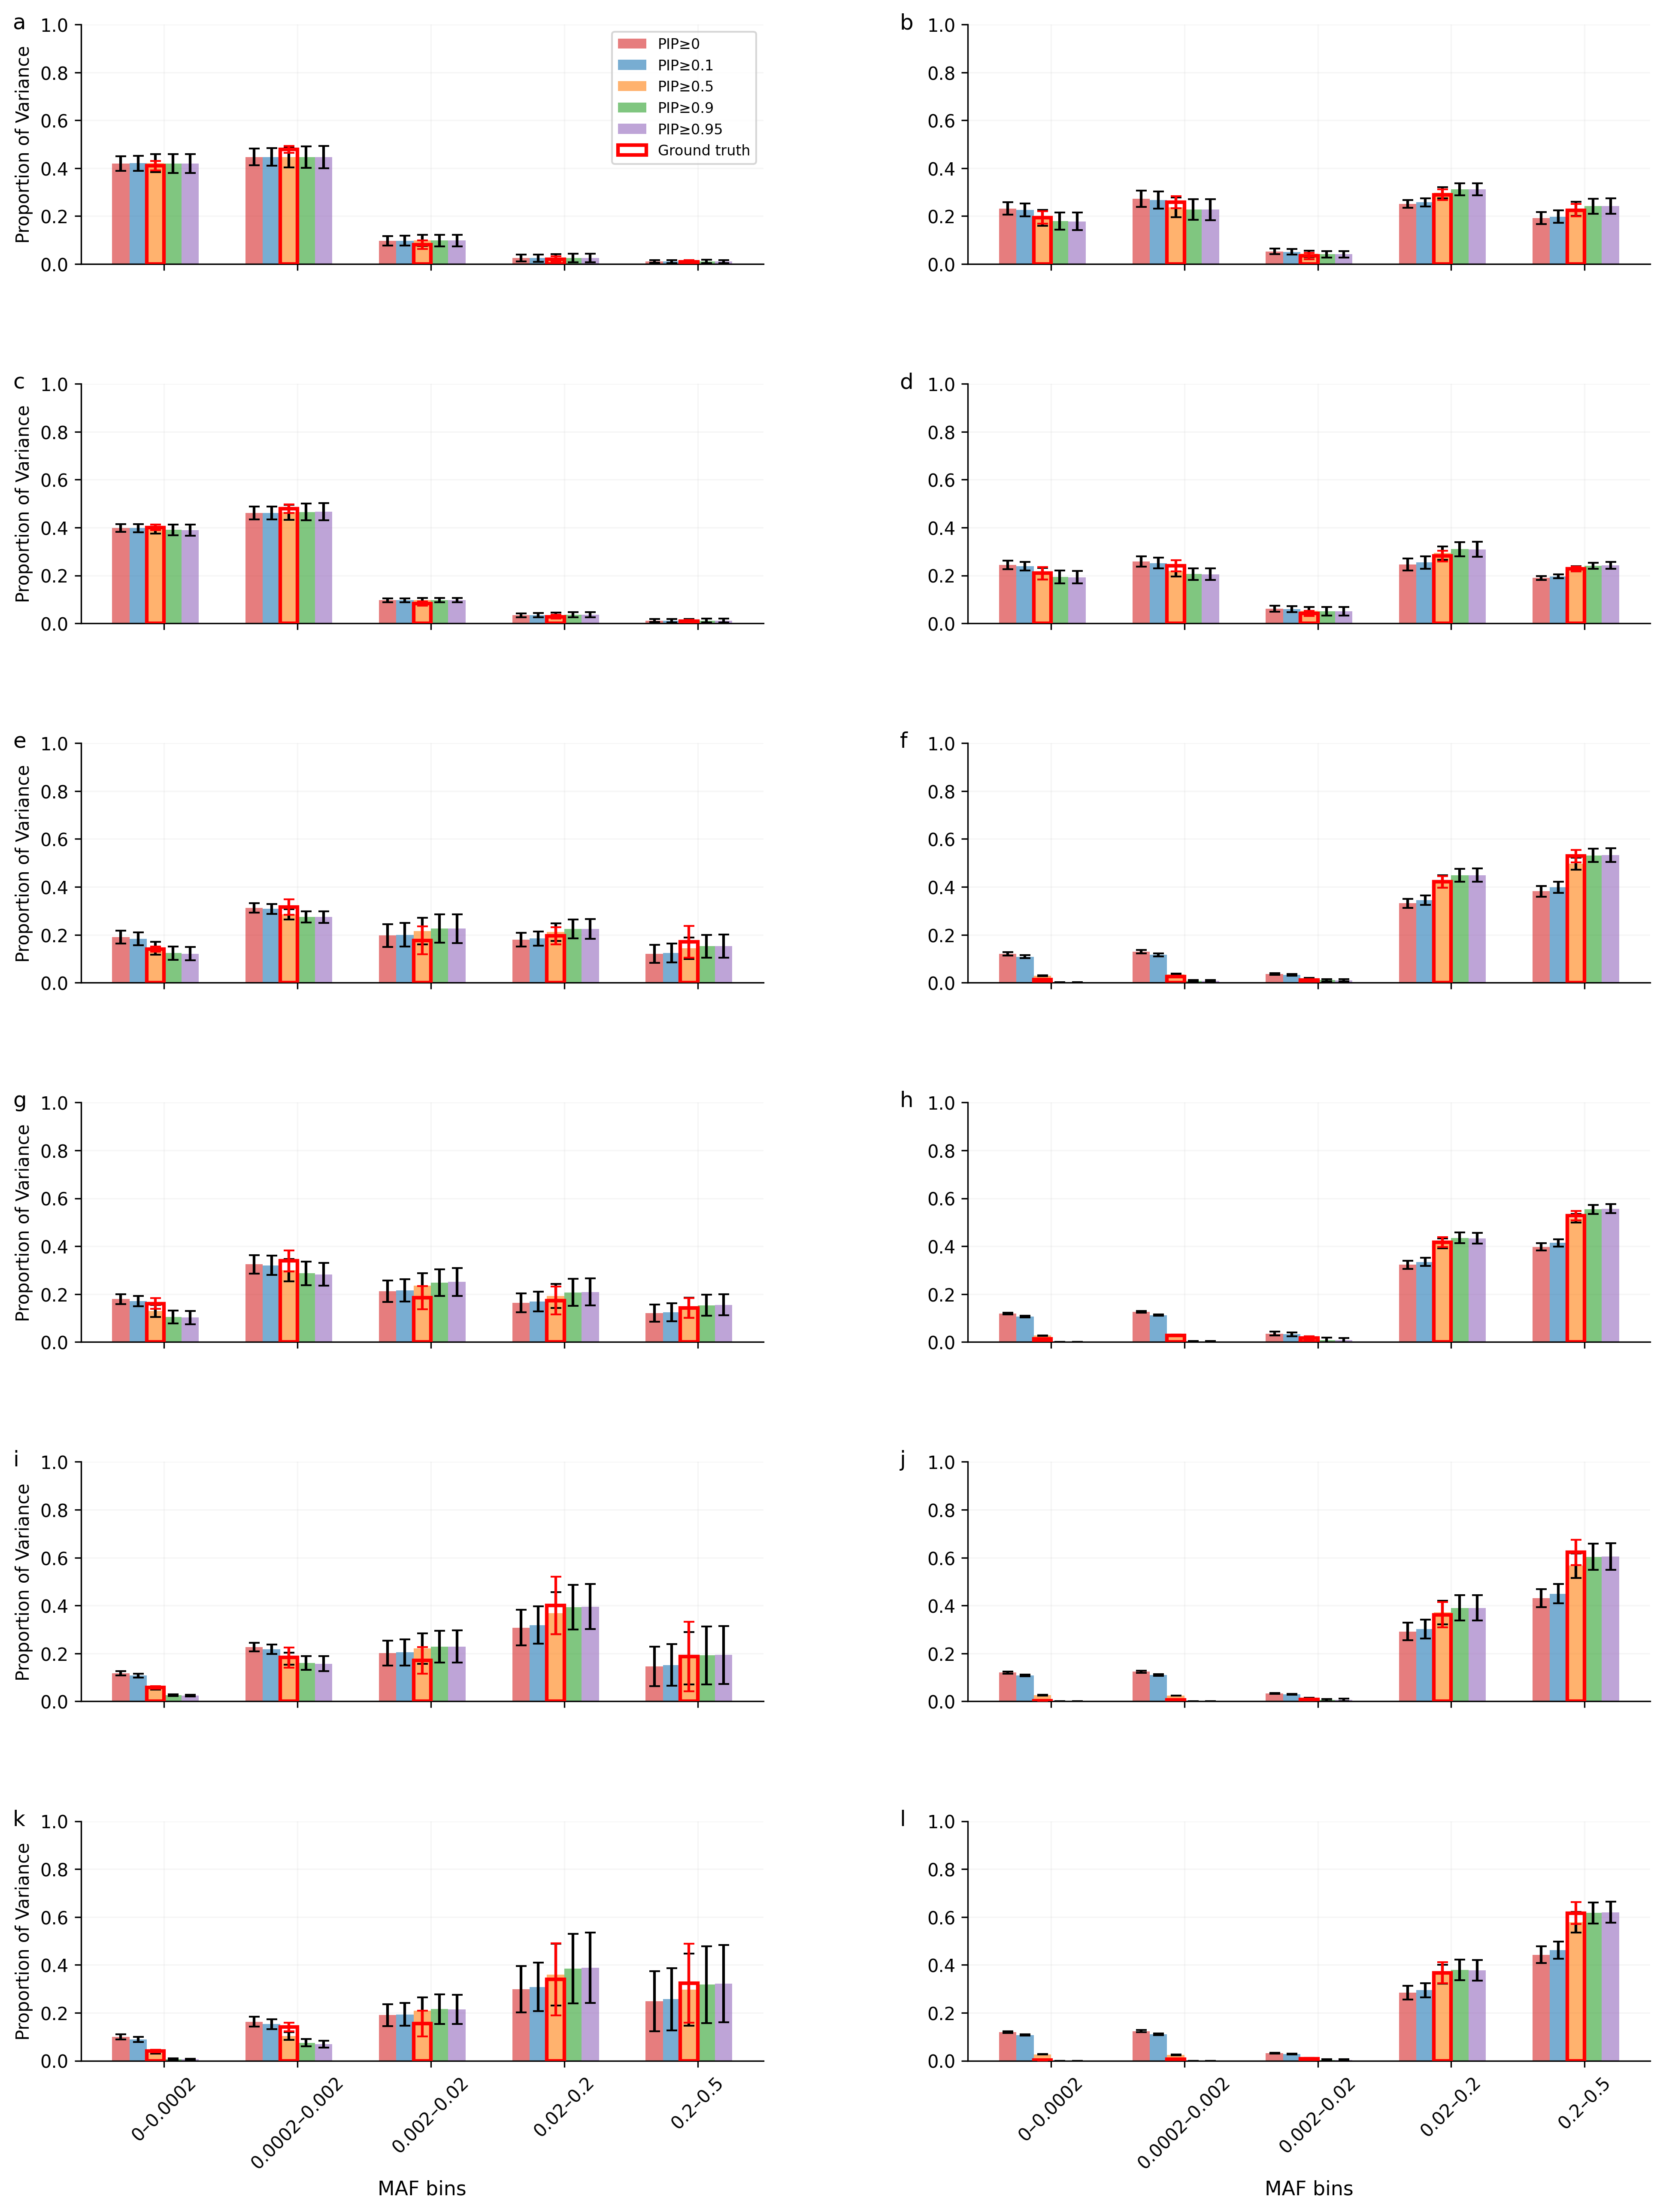
\includegraphics[width=0.9\linewidth]{graphics/gVAMP_figures/v4/FigS5.png}
    \caption[The proportion of variance attributable to DNA loci of different frequency in a whole genome sequence data simulation study using chromosomes 11 to 15 of the UK Biobank]{\textbf{The proportion of variance attributable to DNA loci of different frequency in a whole genome sequence (WGS) data simulation study using chromosomes 11 to 15 of the UK Biobank}. \small We plot the proportion of the sum of the squared regression coefficients attributable to variants of different frequency as estimated from gVAMP across different posterior inclusion probability (PIP) thresholds. The ground truth (red frame) is calculated as the sum of squared true effects across different frequency groups. The variance attributable to SNPs of different frequency matches the ground truth when selecting variants at posterior inclusion probability $\geq 0.5$. Error bars give the standard deviation across 5 simulation replicates.}
    \label{fig:finalFigS4}
\end{figure}

\newpage

\begin{figure}[!htp]
    \centering
    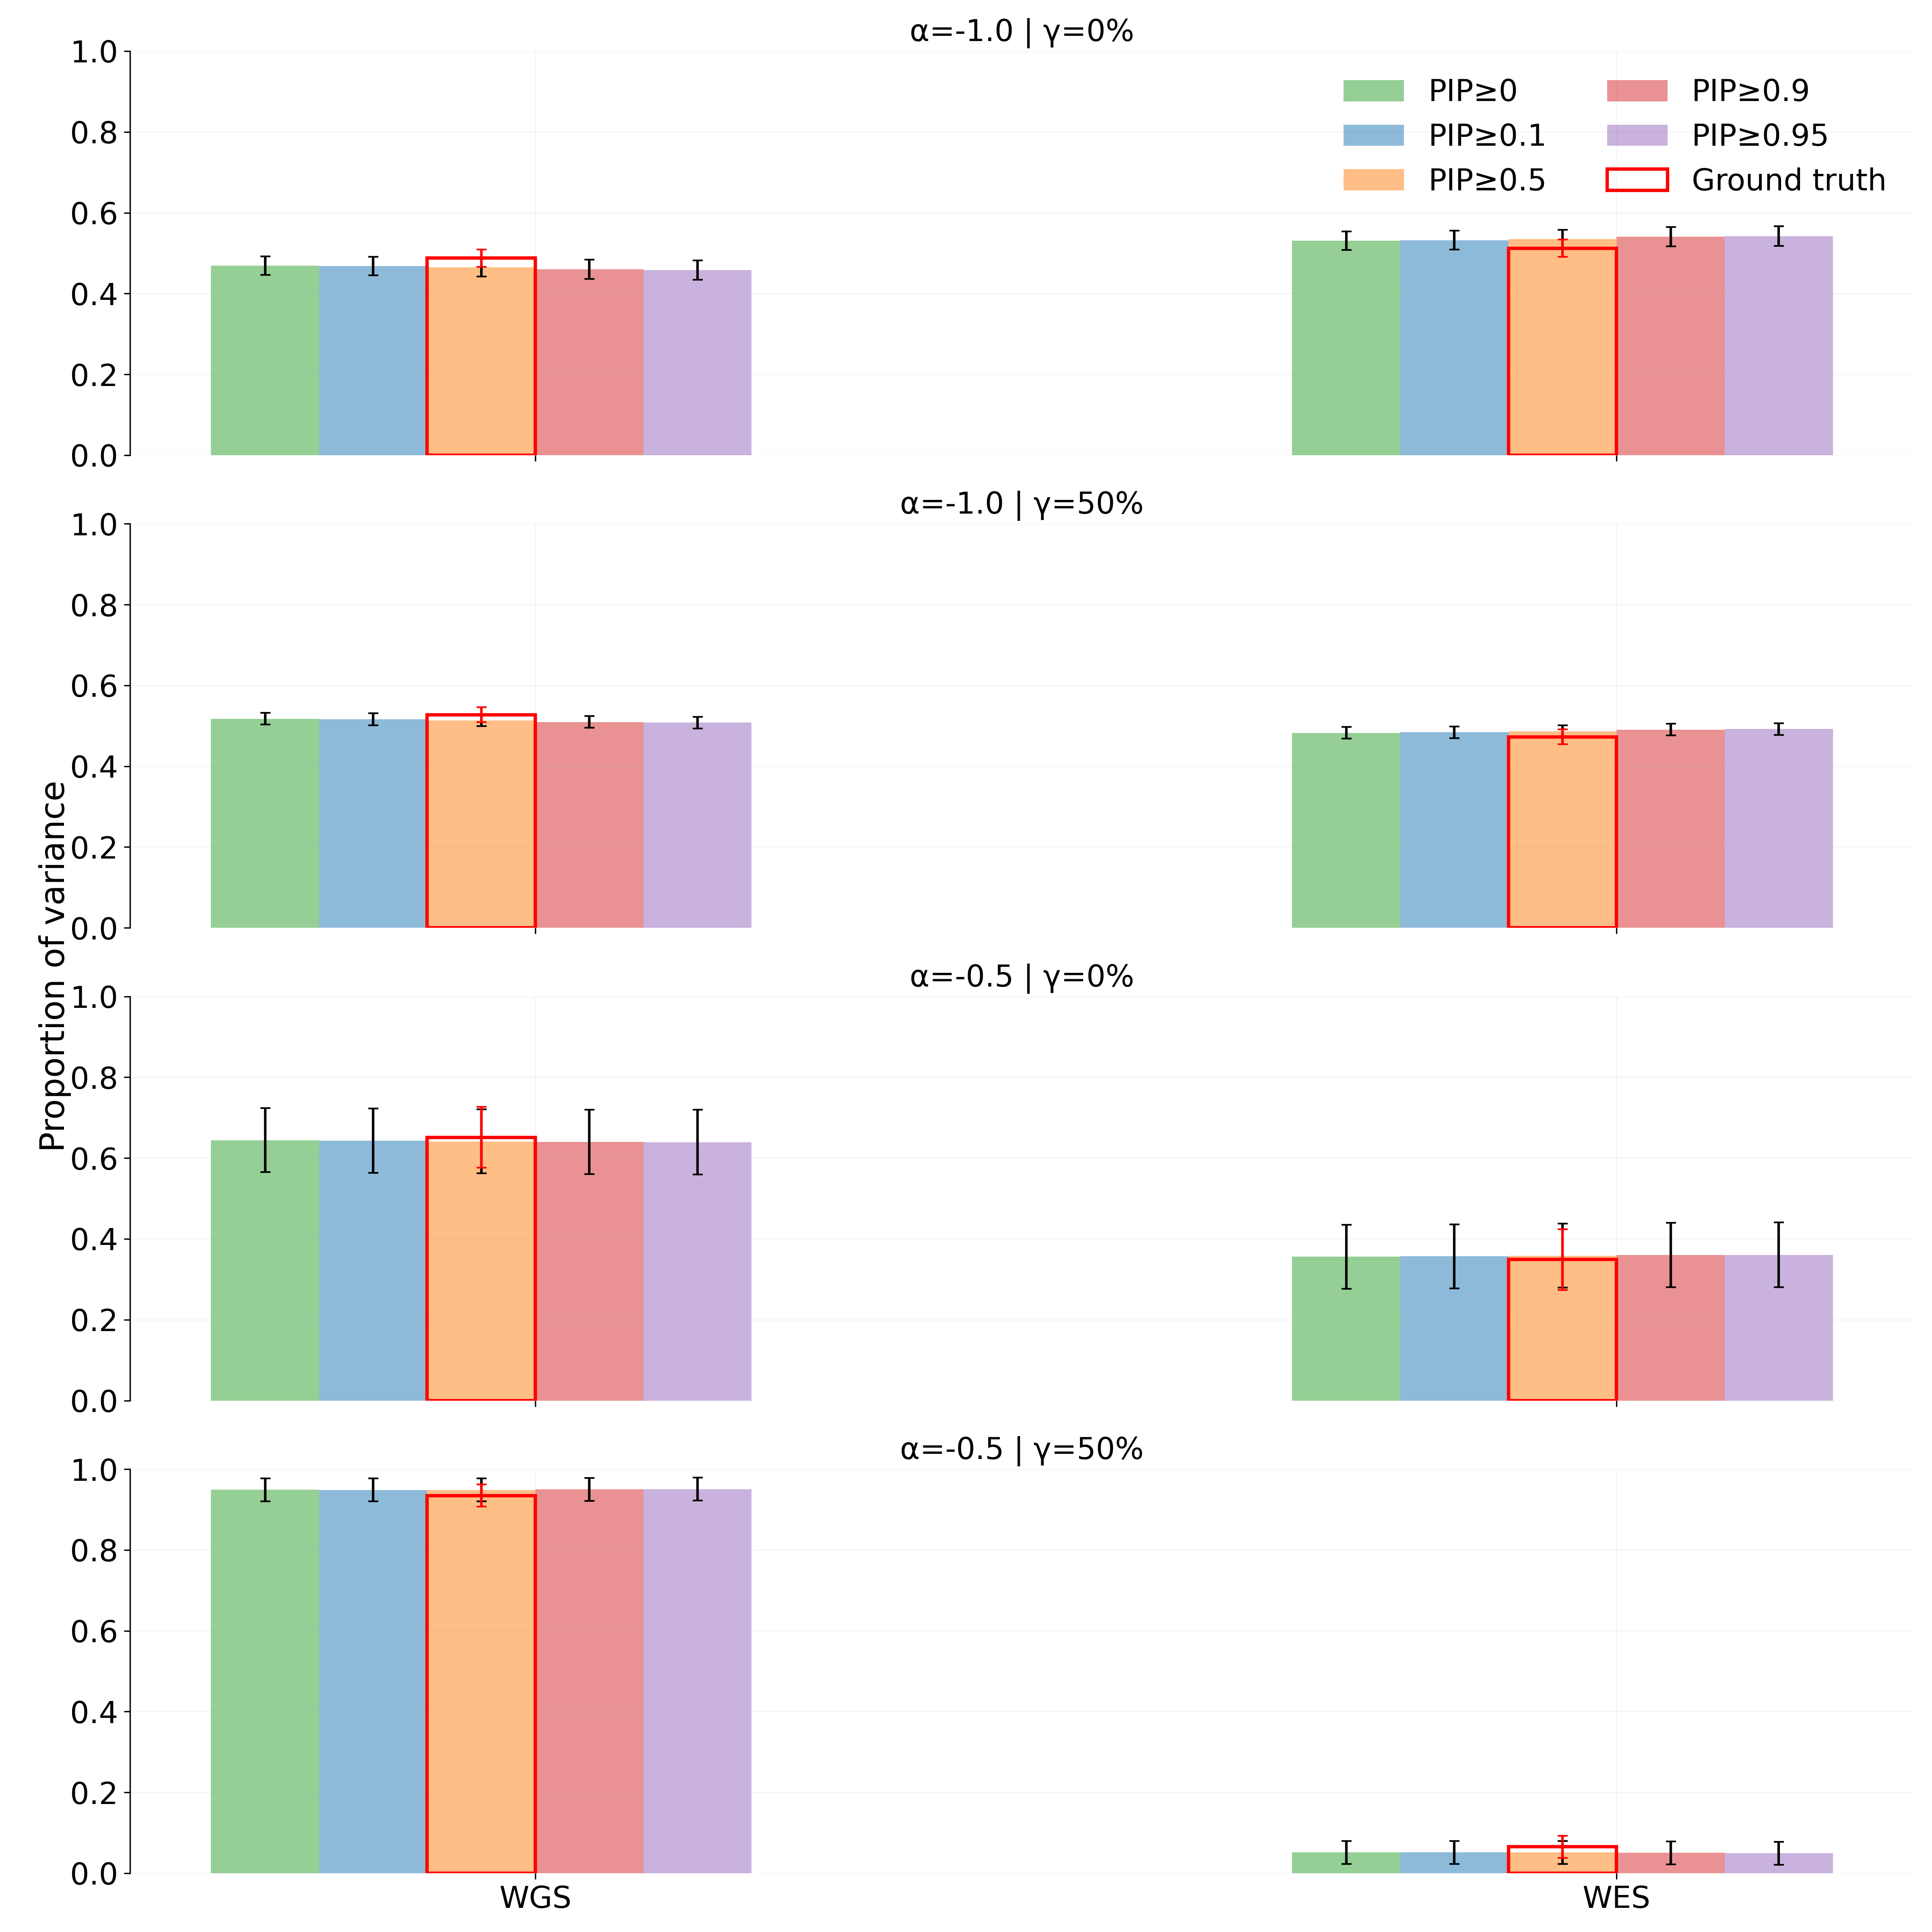
\includegraphics[width=\linewidth]{graphics/gVAMP_figures/v4/FigS6.png}
    \caption[Simulation study including whole exome sequence (WES) burden scores alongside WGS variants from chromosomes 11 to 15 of the UK Biobank]{\textbf{Simulation study including WES burden scores alongside WGS variants from chromosomes 11 to 15 of the UK Biobank}. We simulate 500 underlying causal signals with a total heritability of $h^2=7.25\%$, allocating 75\% of signals to WGS variants and 25\% to WES burden scores, with WES burden scores exhibiting effect sizes three-fold larger than those of individual WGS variants. For the detailed description of $\alpha$ and $\gamma$ parameters, see Methods. We find that the variance explained by WES and WGS, as inferred by gVAMP, aligns well with the ground truth across a range of PIP thresholds.}
    \label{fig:S6}
\end{figure}

\newpage

\begin{figure}[H]
    \centering
    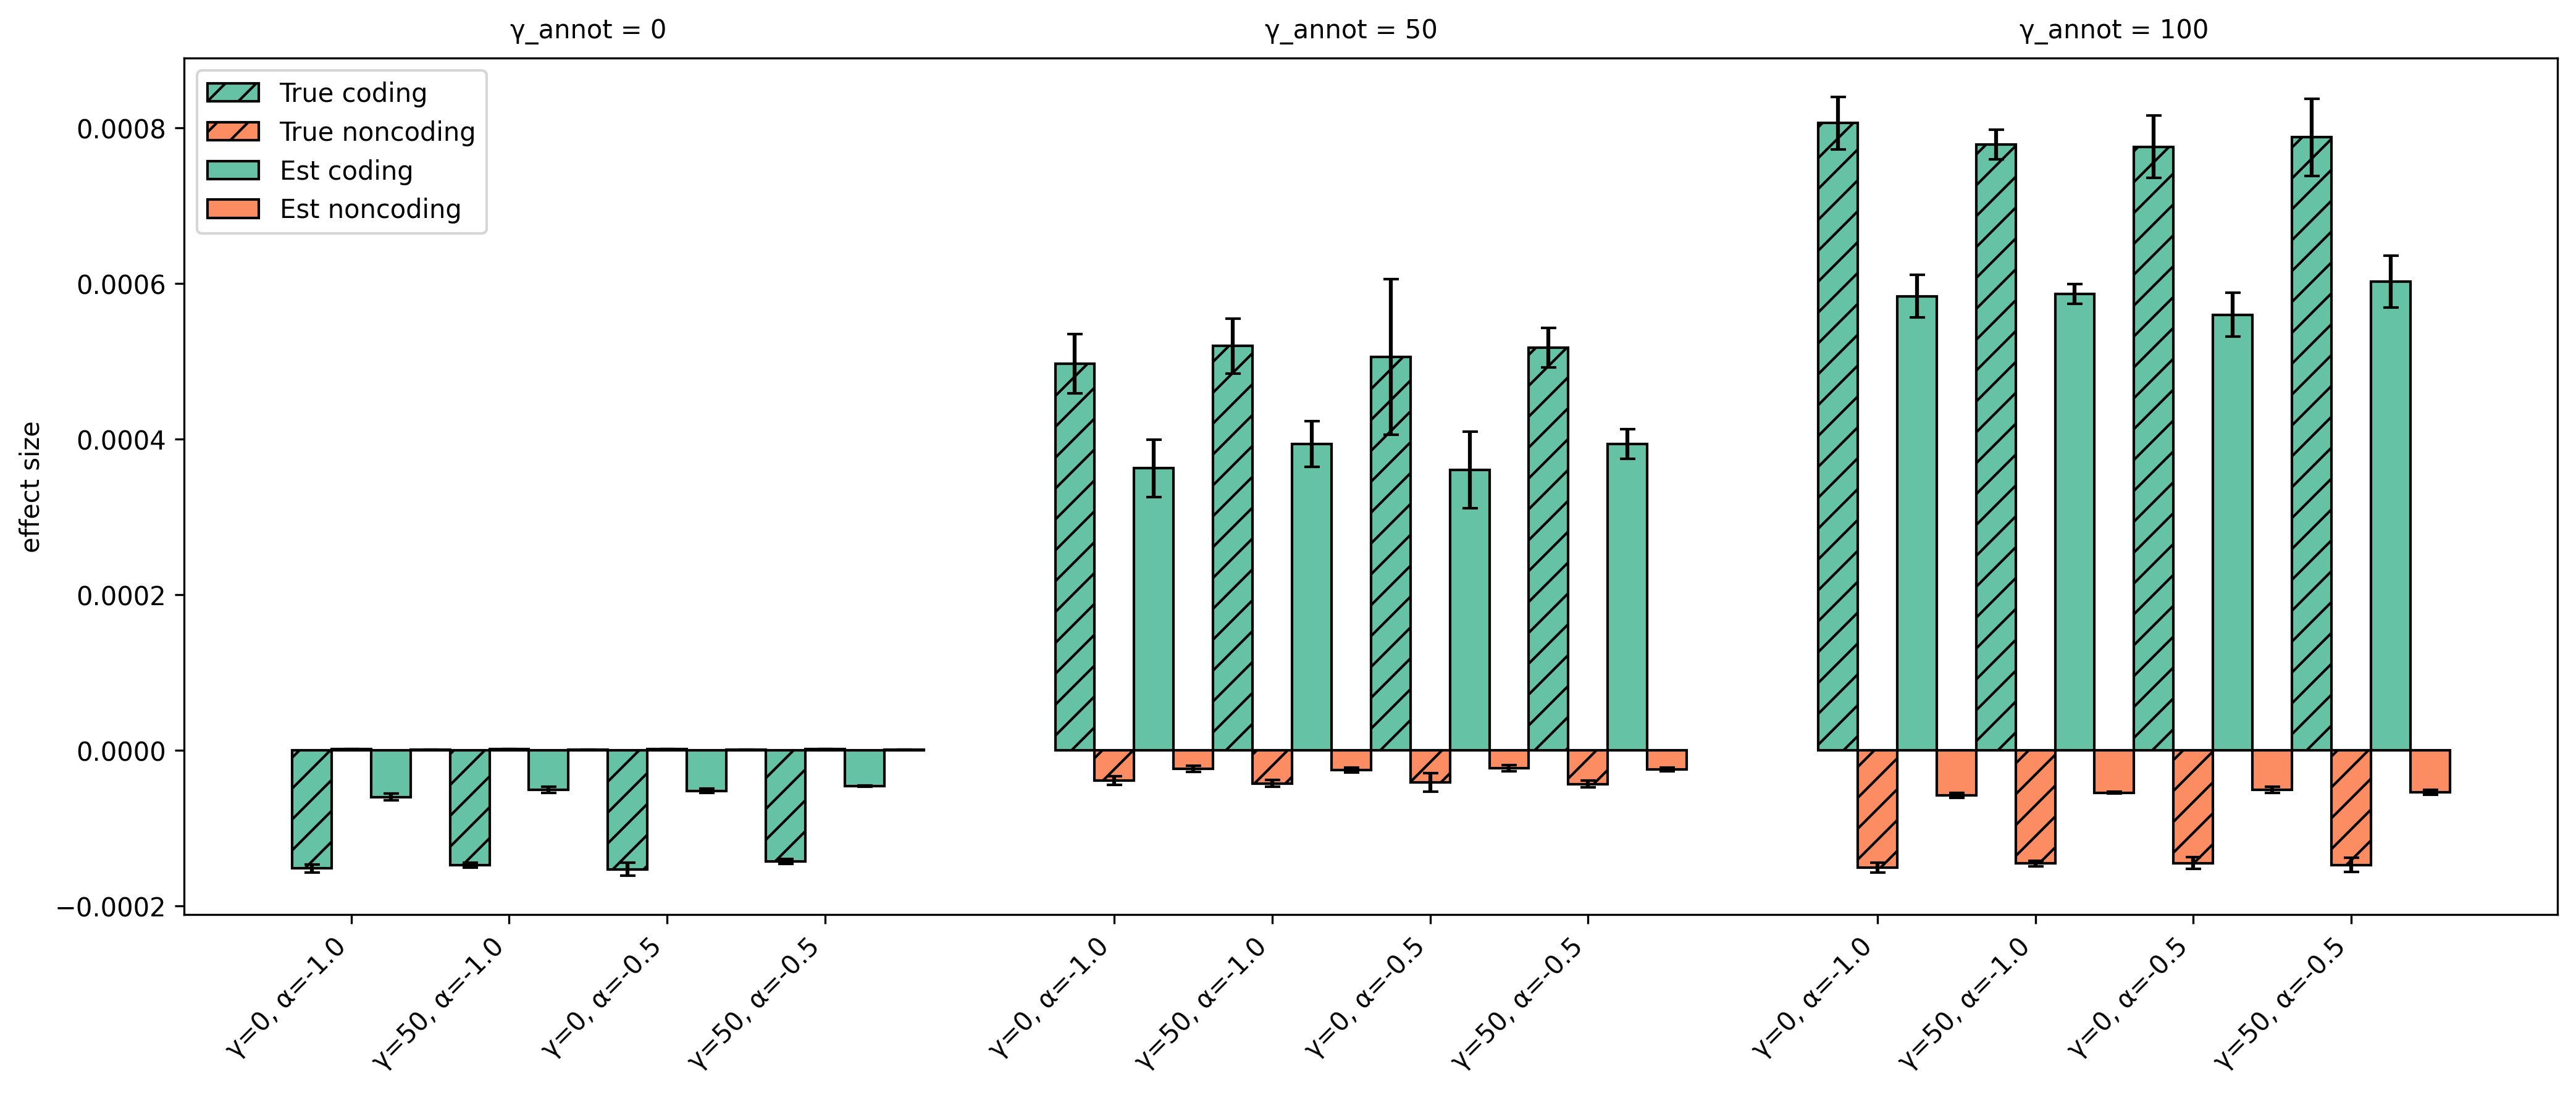
\includegraphics[width=\linewidth]{graphics/gVAMP_figures/cellgen_review/effect_size_plot_threshold_0.0.png}
    \caption[Simulation study stratifying causal effects into coding and non-coding regions]{\textbf{Simulation study stratifying causal effects into coding and non-coding regions.} We simulate 500 signals with a total heritability of $h^2=7.25\%$ across a variety of settings for power law $\alpha$ and percentage of common variants $\gamma$, also allocating $\gamma_\text{annot} \in \{0, 50, 100 \}$ \% percentage of causal variants to the coding region of the DNA. Effect sizes ($y$-axis) are calculated as the difference of the group average absolute value of the effects from the total group average absolute value of the effect (enrichment). The true simulated values are given by boxes with diagonal lines.}
    \label{fig:S7new}
\end{figure}

\newpage

\begin{figure}[!htp]
    \centering
    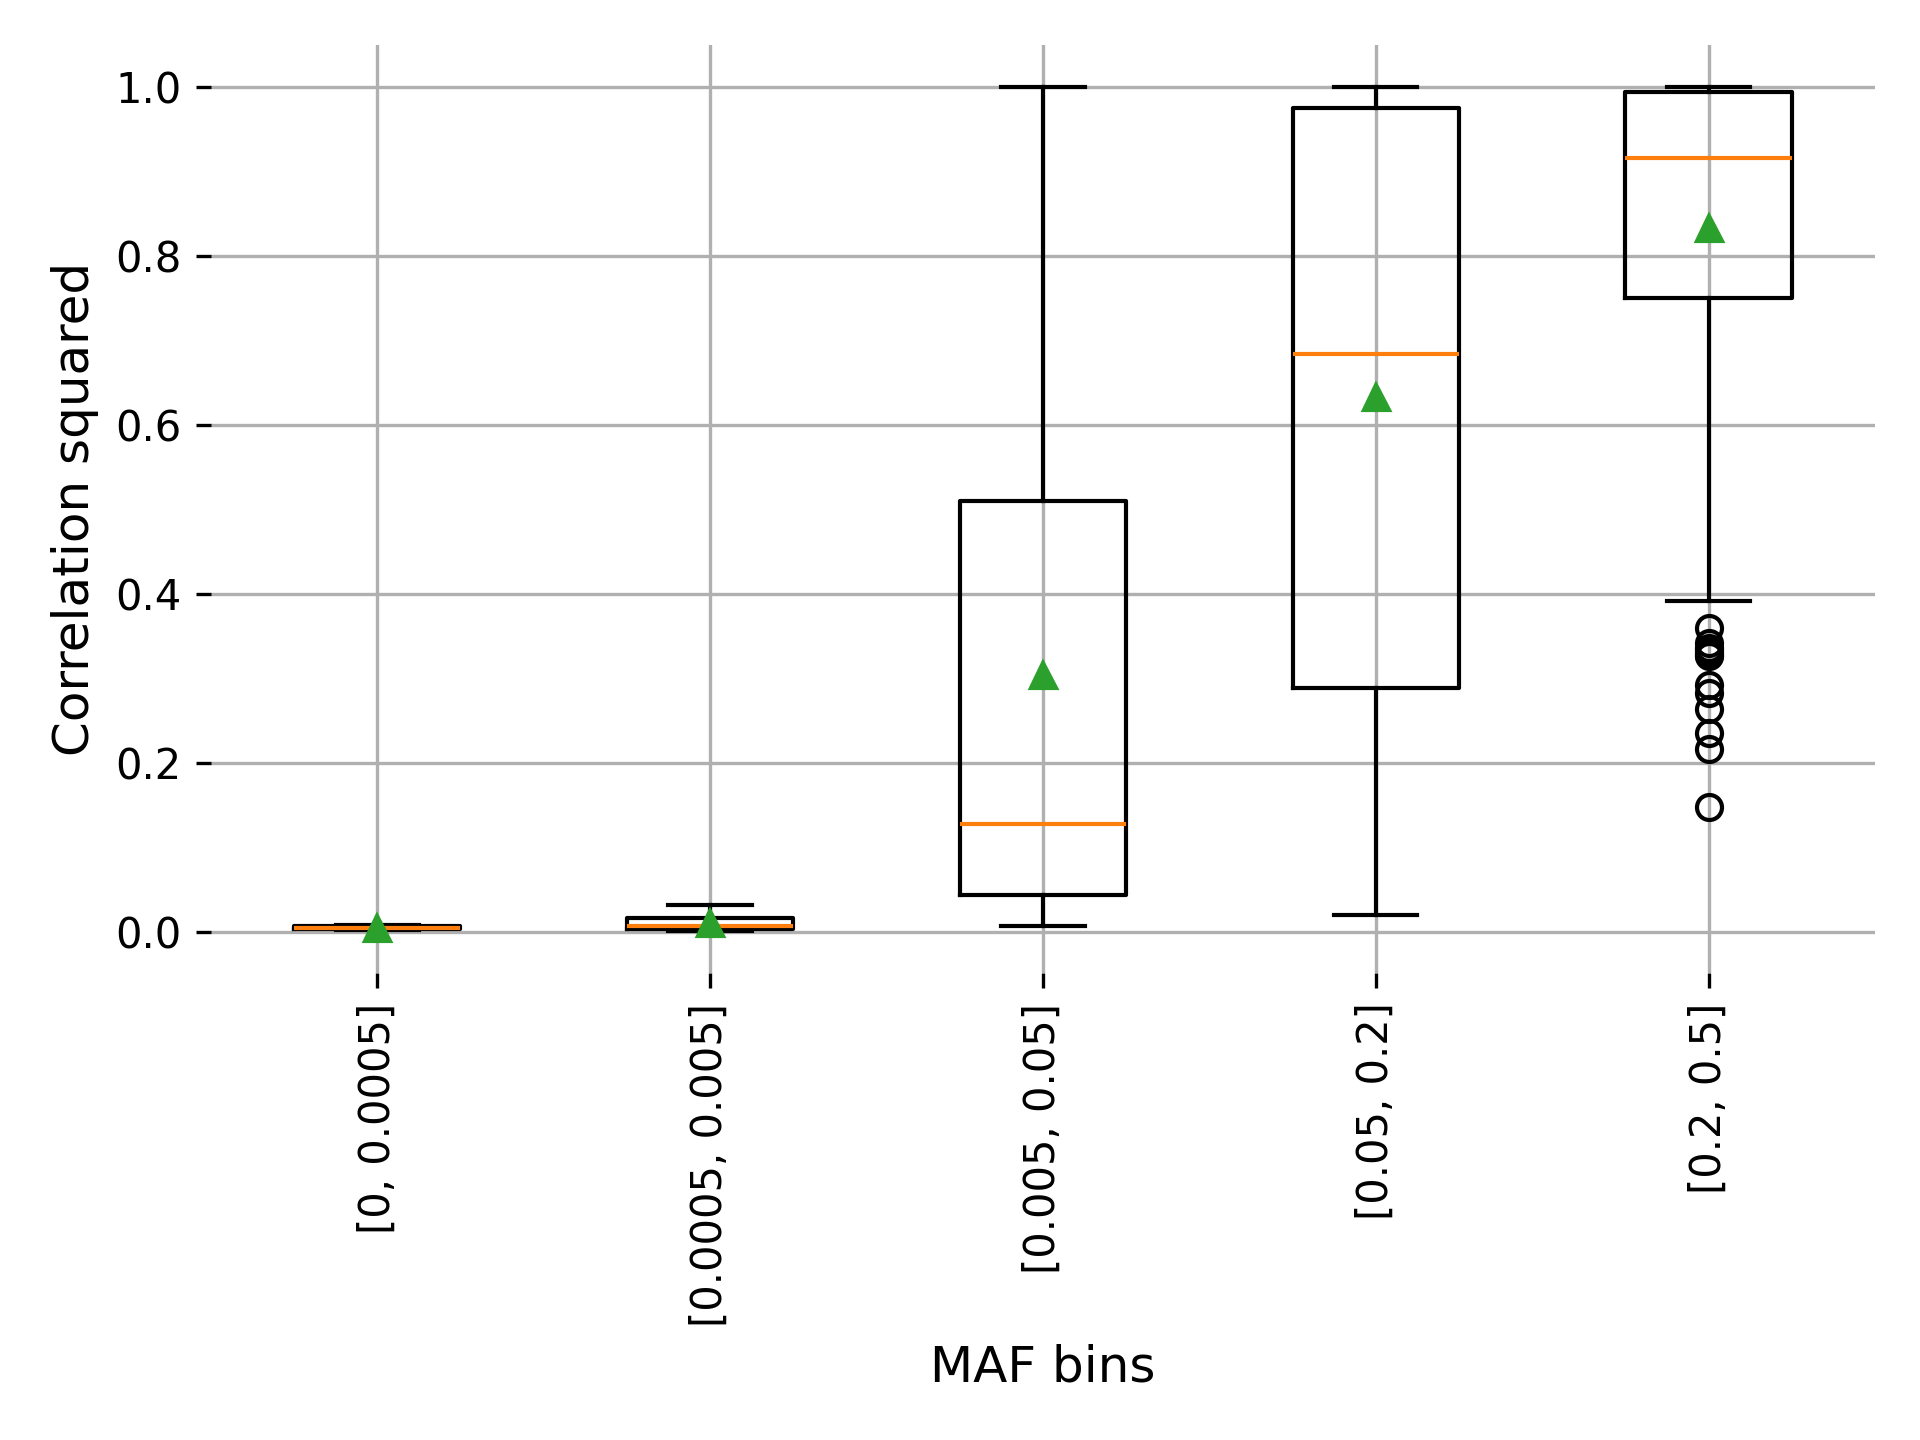
\includegraphics[width=\linewidth]{graphics/gVAMP_figures/v4/FigS8.png}
    \caption[Distribution of the maximum squared correlation between each height-associated variant found by gVAMP and variants reported by Yengo \textit{et al.} \cite{HTbig} within a 1Mb window across MAF groups]{\textbf{Distribution of the maximum squared correlation between each height-associated variant found by gVAMP and variants reported by Yengo \textit{et al.} \cite{HTbig} within a 1Mb window across MAF groups.} We estimate the maximum correlation within the UK Biobank WGS data of each gVAMP discovery at PIP$\geq95\%$ with Yengo \emph{et al.} SNPs significant at $p\le5 \cdot 10^{-8}$ within a 1 Mb window and stratify the squared correlations by the MAF of the gVAMP discovered variant. The orange line depicts the median, while the green triangle indicates the mean value. In total, we find 432 SNPs with correlation squared greater than 0.1. The results suggest that very rare variants (MAF $\le 0.005$) are independent of the colocalizing common variants from \cite{HTbig}.}
    \label{fig:correlation_MAF}
\end{figure}

\newpage

\begin{figure}[!htp]
    \centering
    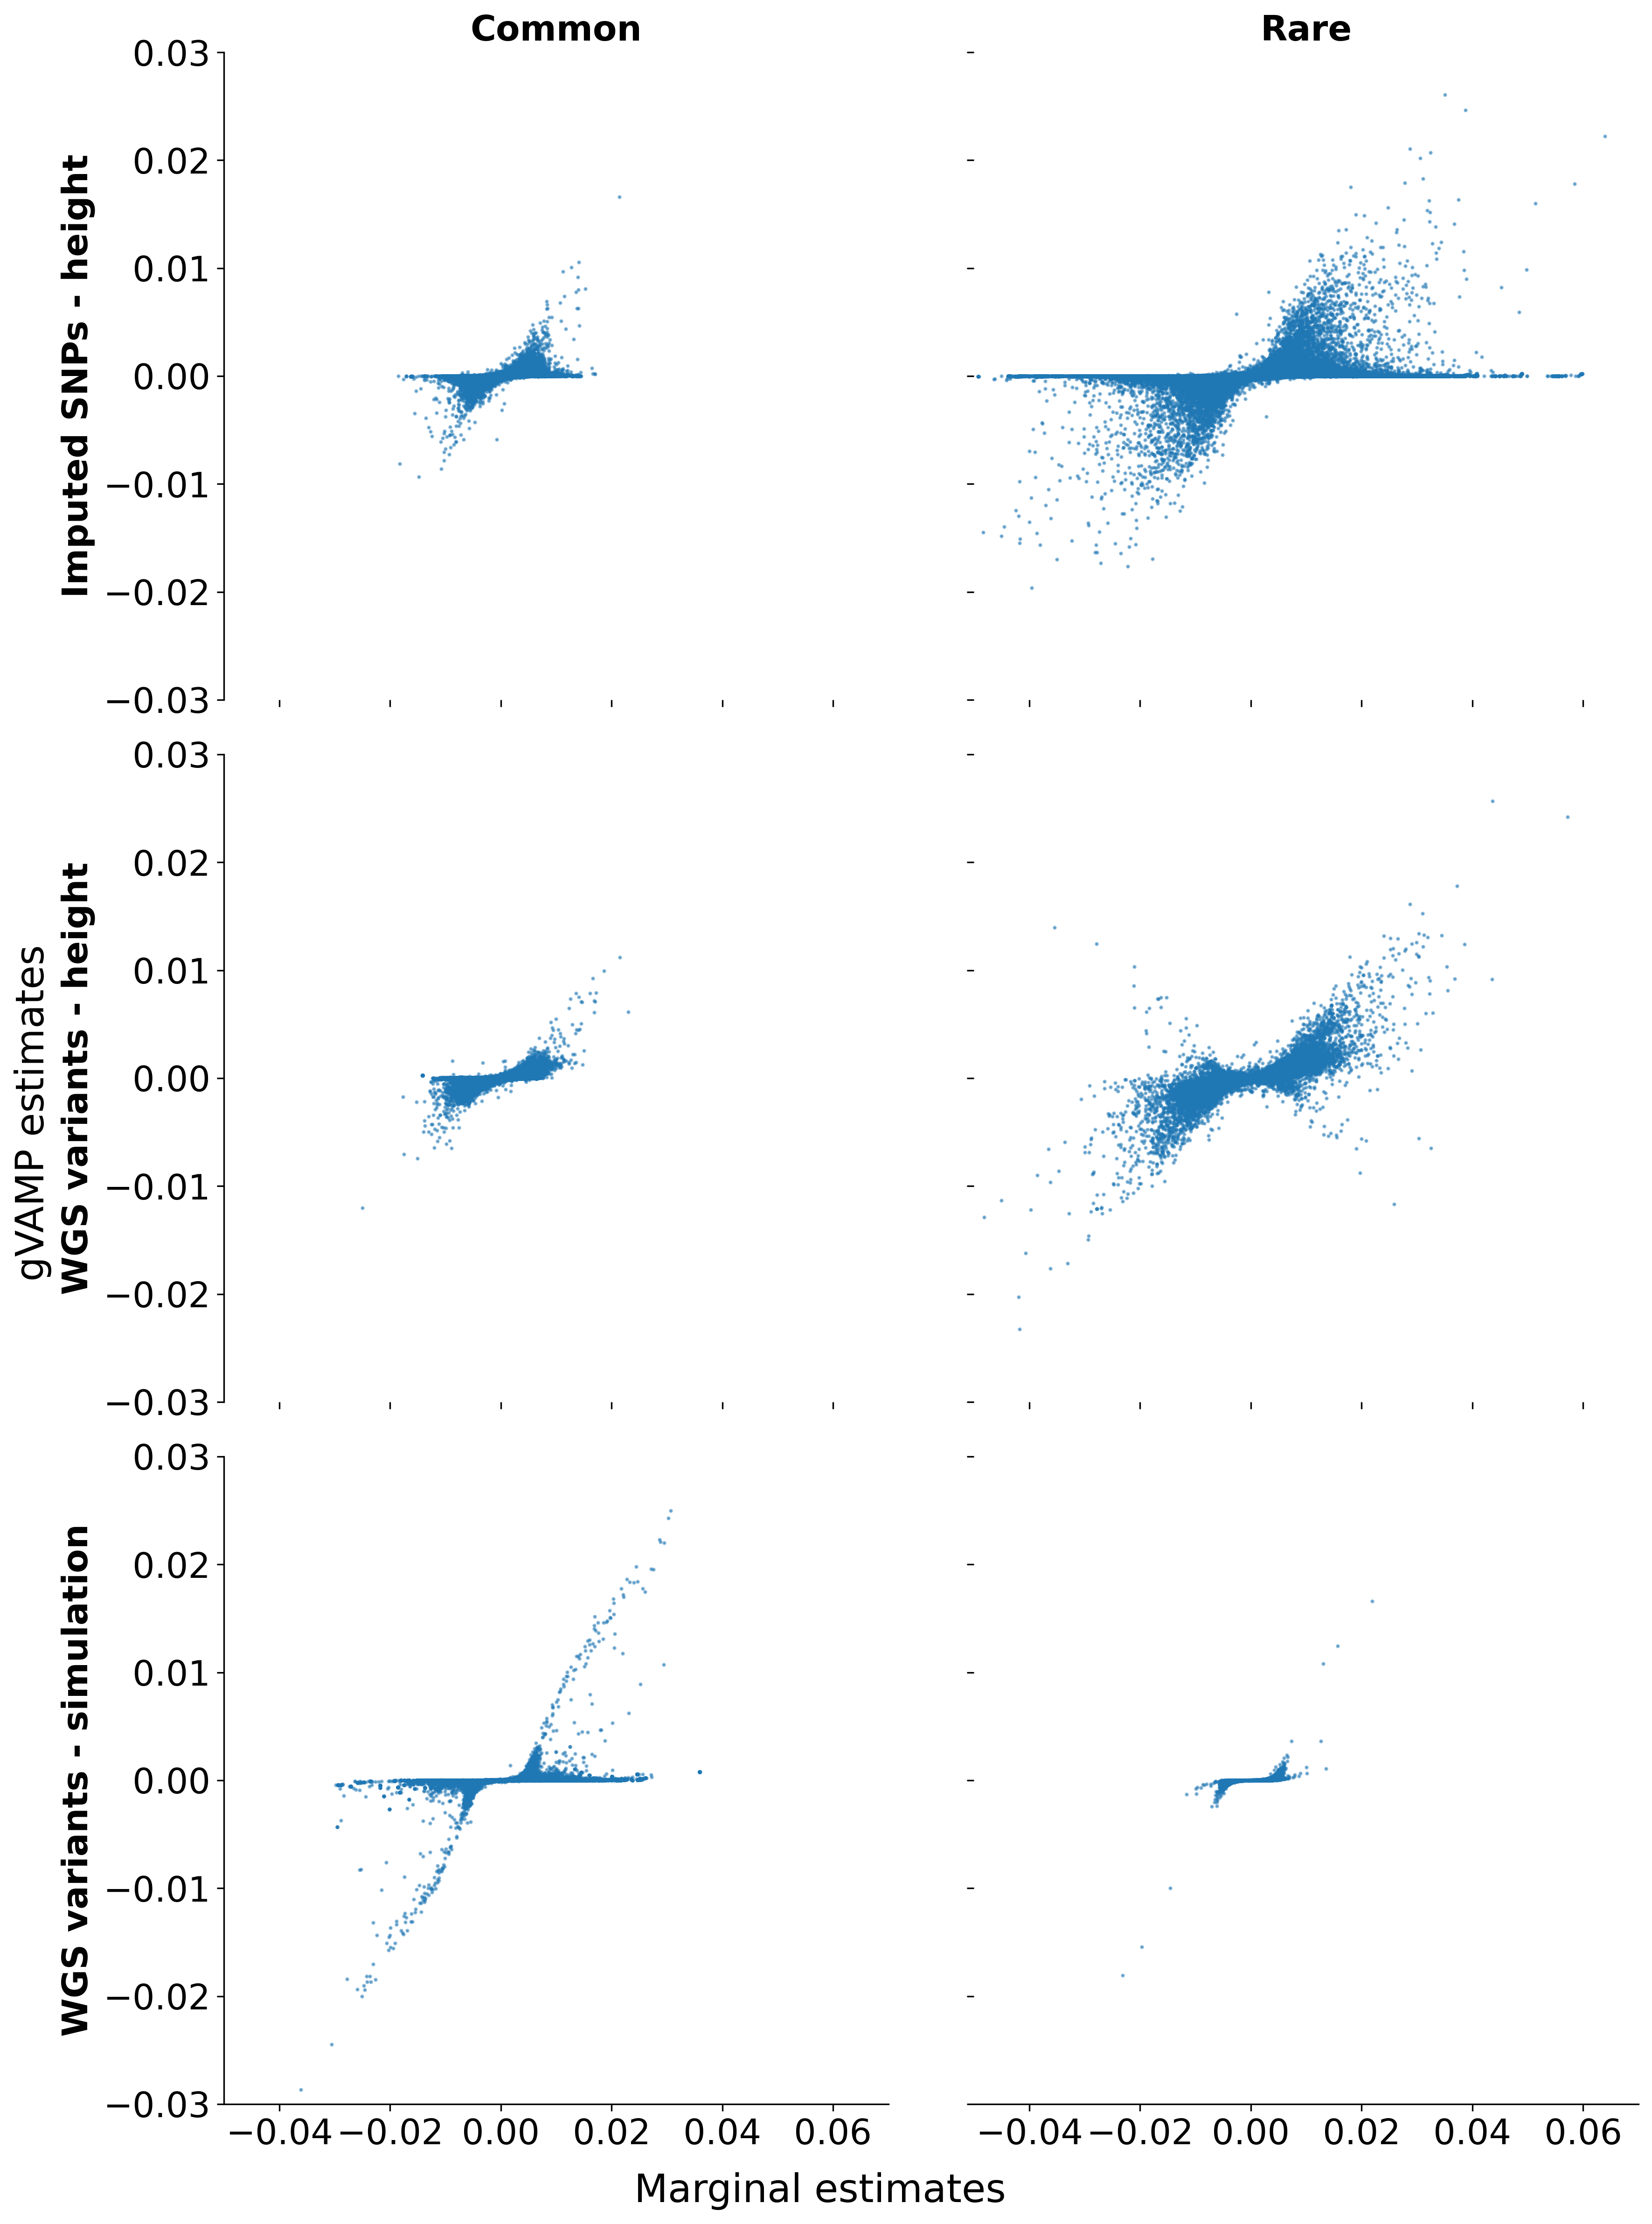
\includegraphics[width=\linewidth]{graphics/gVAMP_figures/v4/FigS9.png}
    \caption[Marginal regression coefficient estimates of the relationship of 16,854,878 whole genome sequence variants with human height, plotted against the regression coefficient values obtained from gVAMP]{\textbf{Marginal regression coefficient estimates of the relationship of 16,854,878 whole genome sequence (WGS) variants with human height, plotted against the regression coefficient values obtained from gVAMP}.}
    \label{fig:figS8}
\end{figure}

\begin{figure}[!t] % the continued legend, at the top of the page after the figure
    \ContinuedFloat
    \captionsetup{labelformat=continued}
    \caption[]{\small "WGS" refers to the gVAMP run on the WGS variants, "Imputed" refers to the gVAMP run on 8,430,446 imputed SNP markers, and "Simulation" gives the same comparison of marginal and gVAMP estimates in setting $a$. The comparison is plotted for common (minor allele frequency, MAF $\ge 1\%$) and rare variants (MAF $< 1\%$).}
\end{figure}

\newpage

\begin{figure}[!htp]
    \centering
    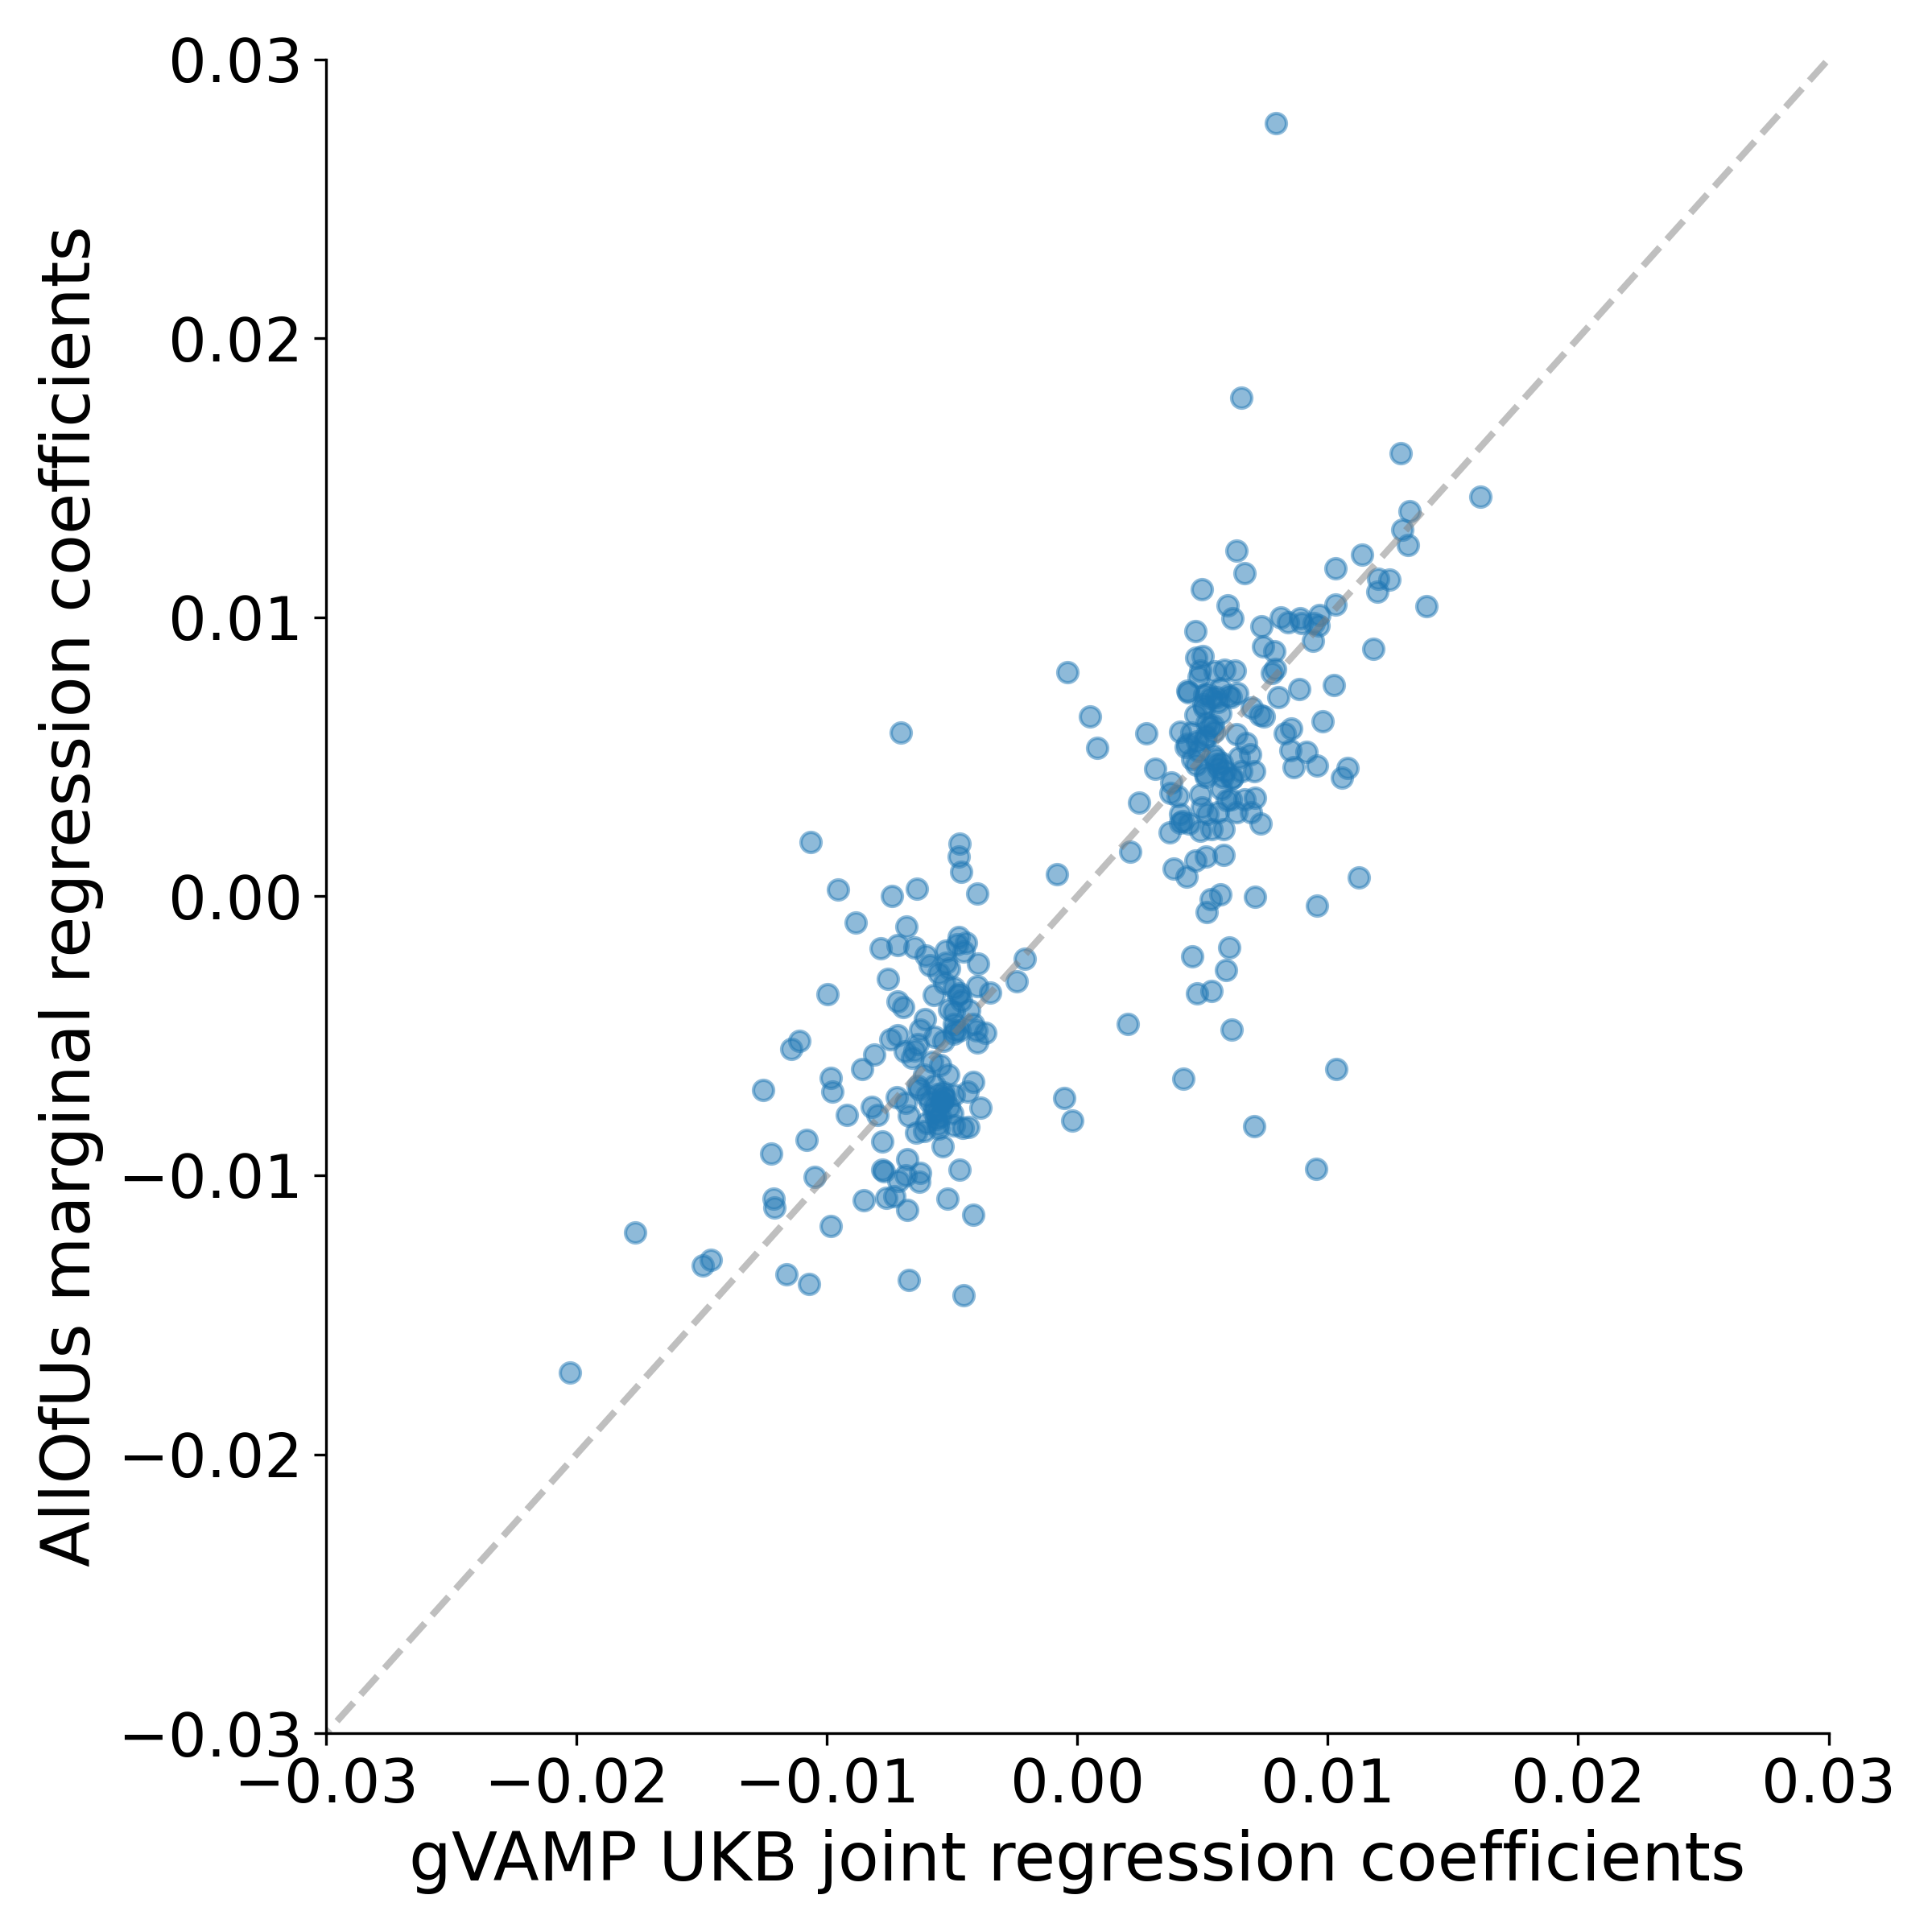
\includegraphics[width=\linewidth]{graphics/gVAMP_figures/v4/FigS10.png}
    \caption[Replication of UK Biobank gVAMP findings in the All of Us dataset]{\textbf{Replication of UK Biobank gVAMP findings in the All of Us dataset.} On the $x$-axis, we plot gVAMP regression coefficient estimates for human height in WGS data discovered at PIP $\geq 0.95$. On the $y$-axis, we plot the marginal regression coefficient estimates of the same SNPs in WGS data in the All of Us dataset, controlling for sex and 16 available PCs. When the major and minor alleles are swapped between two datasets, we change the sign of the effect to match them. The slope of the fitted regression line is $0.8471$.} 
    \label{fig:figS9}
\end{figure}

\newpage

\begin{figure}[!htp]
    \centering
    \includegraphics[width=\linewidth]{graphics/gVAMP_figures/figureS2.png}
    \caption[The variance attributable to gene burden scores calculated from WES data ($y$-axis) shows no relationship to the variance attributable to DNA variants within and around the gene ($x$-axis) estimated from a gVAMP analysis of either 8,430,446 imputed SNP markers or 16,854,878 whole genome sequence variants]{\textbf{The variance attributable to gene burden scores calculated from whole exome sequence (WES) data ($y$-axis) shows no relationship to the variance attributable to DNA variants within and around the gene ($x$-axis) estimated from a gVAMP analysis of either 8,430,446 imputed SNP markers or 16,854,878 whole genome sequence (WGS) variants.}}
    \label{fig:figS10}
\end{figure}


\newpage


\begin{figure}[!htp]
    \centering
    \includegraphics[width=0.88\linewidth]{graphics/gVAMP_figures/old_figs/Figure_S3.png}
    \caption[SNP heritability estimation of GMRM versus gVAMP with different numbers of SNP markers across 13 traits in the UK Biobank]{\textbf{SNP heritability estimation of GMRM versus gVAMP with different numbers of SNP markers across 13 traits in the UK Biobank.} \small Comparison of the proportion of phenotypic variation attributable to 2,174,071 autosomal SNP genetic markers (SNP heritability) estimated by GMRM ($x$-axis) to the SNP heritability estimated by gVAMP ($y$-axis) at either the same 2,174,071 SNPs (red) or 8,430,446 SNP markers (blue). The slope of the lines shows a 1-to-1 relationship of gVAMP to GMRM, but with an average of 3.4\% lower estimate for gVAMP at 2.17M SNPs. Analyzing 8.4M SNPs with gVAMP increases the heritability estimate over GMRM by 3.9\%, which is consistent with an increase in phenotypic variance captured by the full imputed sequence data, as opposed to a selected subset of SNP markers. The dashed grey line gives $y=x$.}
    \label{fig:figS12}
\end{figure}

\newpage


% \section*{Supplementary Note 1}
\refstepcounter{suppnotegvamp}
% \section{Supplementary Note \thesuppnotegvamp}
\section{Prediction accuracy and association testing simulations using imputed UK Biobank data}
\label{supp:note1}

\begin{figure}[!htp]
    \centering   
    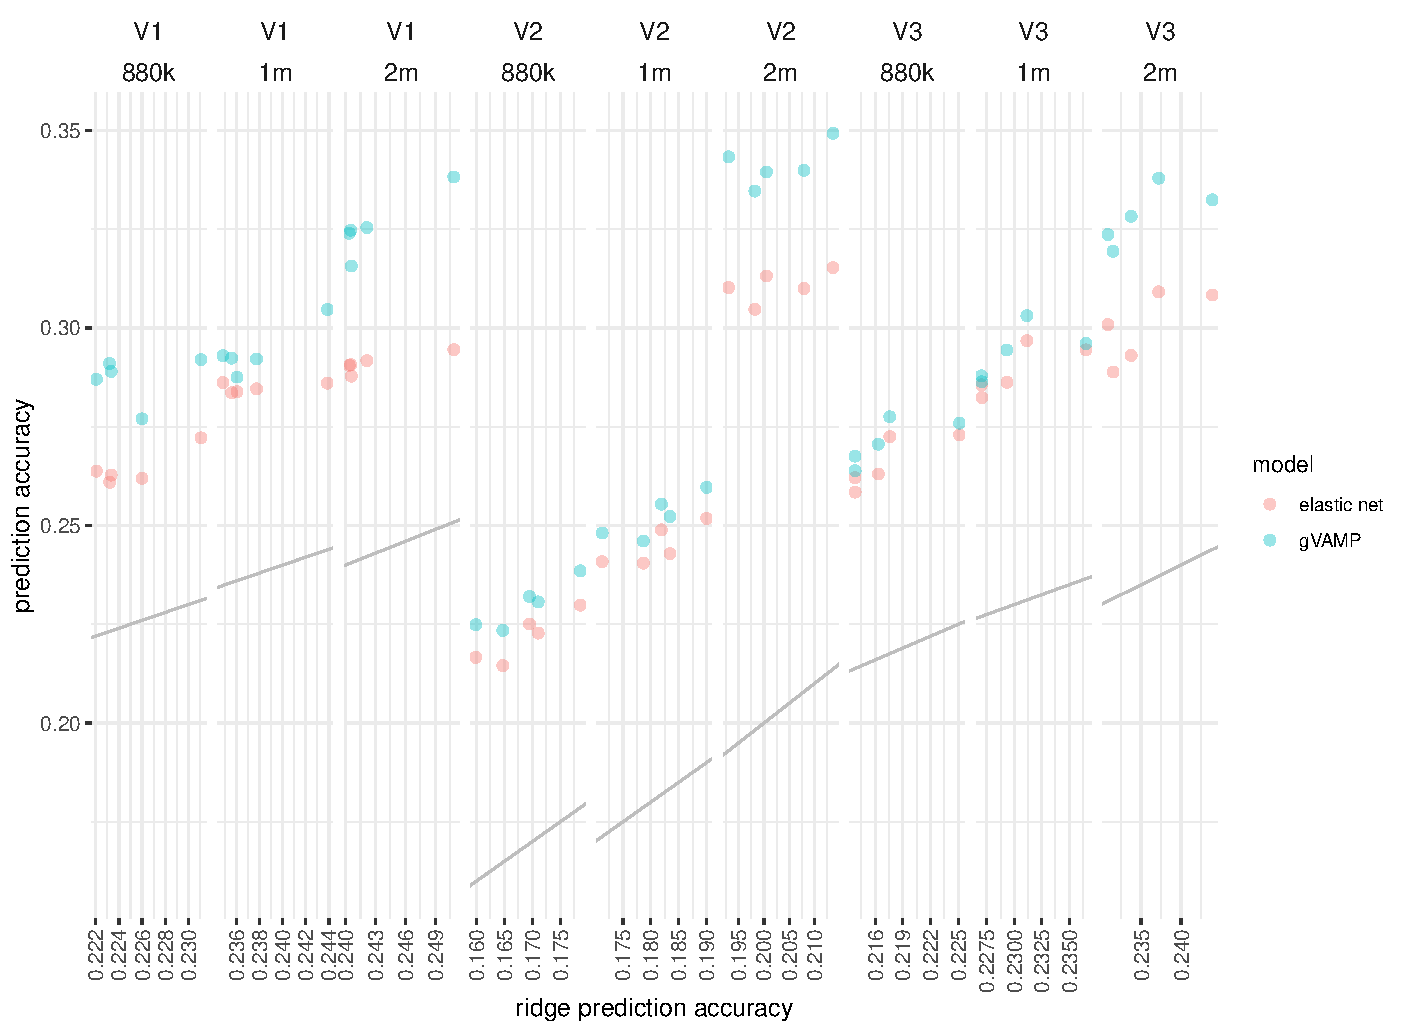
\includegraphics[width=\linewidth]{graphics/gVAMP_figures/Fig_SN1.pdf}
    \caption[Simulation study of out-of-sample prediction accuracy in UK Biobank imputed genotype data]{\textbf{Simulation study of out-of-sample prediction accuracy in UK Biobank imputed genotype data.} \small{We compare out-of-sample prediction accuracy ($y$-axis) for polygenic risk scores (PRS) created at different sets of markers ("880k" = 887,060, "1m" = 1,410,525, "2m" = 2,174,071 SNPs) from gVAMP (blue) and an elastic net model implemented in the LDAK software (red), as compared to the prediction accuracy obtained at the same sets of SNPs from a ridge regression model implemented in the LDAK software ($x$-axis). Grey lines give the 1:1 line. Comparisons are made across three settings: "V1" where 40,000 causal variants are randomly selected from 8,430,446 SNP markers and effects are drawn from a Gaussian, "V2" where 40,000 causal variants are randomly selected from 8,430,446 SNP markers, with effects that have a power relationship to the minor allele frequency of -0.5, and "V3" where 40,000 causal variants are randomly selected from 8,430,446 SNP markers, with effects drawn from an elastic net distribution.}}
    \label{fig:figSN1}
\end{figure}

\begin{figure}[!htp]
    \centering   
    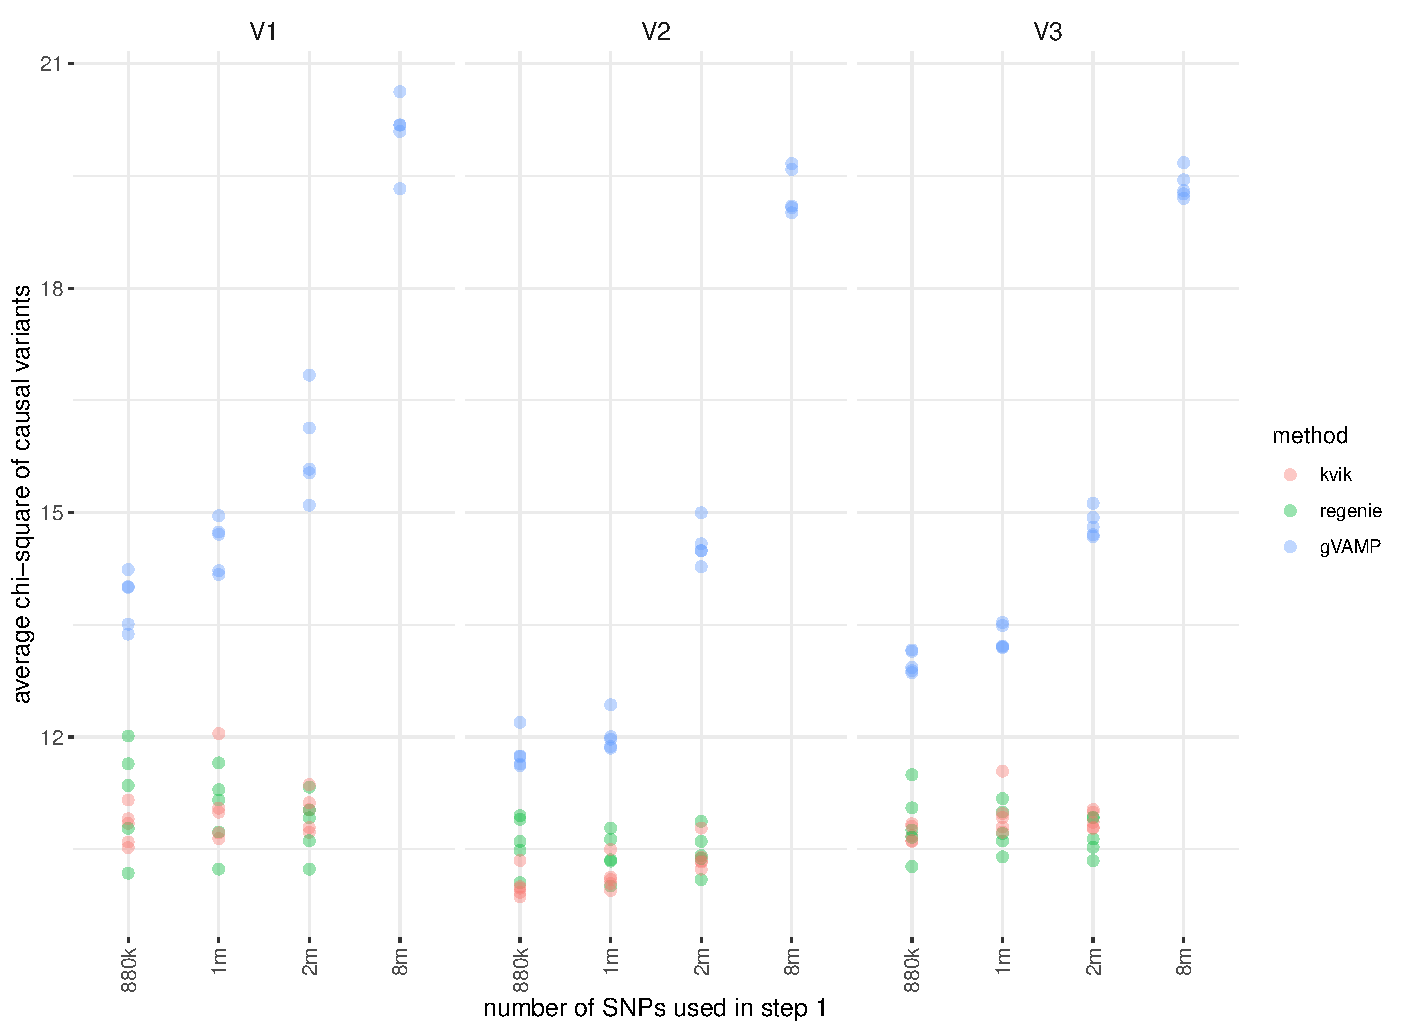
\includegraphics[width=\linewidth]{graphics/gVAMP_figures/Fig_SN2.pdf}
    \caption[Simulation study of power for mixed linear model leave-one-chromosome out association testing in UK Biobank imputed genotype data]{\textbf{Simulation study of power for mixed linear model leave-one-chromosome out association testing in UK Biobank imputed genotype data.} \small{We compare the average chi-squared value at the causal variants ($y$-axis) for leave-one-chromosome-out association testing (LOCO) when the first step LOCO predictors are created at different sets of markers ("880k" = 887,060, "1m" = 1,410,525, "2m" = 2,174,071 SNPs) from gVAMP (blue), an elastic net model implemented in the LDAK software (red), and Regenie (green). Comparisons are made across three settings: "V1" where 40,000 causal variants are randomly selected from 8,430,446 SNP markers and effects are drawn from a Gaussian, "V2" where 40,000 causal variants are randomly selected from 8,430,446 SNP markers, with effects that have a power relationship to the minor allele frequency of -0.5, and "V3" where 40,000 causal variants are randomly selected from 8,430,446 SNP markers, with effects drawn from an elastic net distribution.}}
    \label{fig:figSN2}
\end{figure}

\begin{figure}[!htp]
    \centering   
    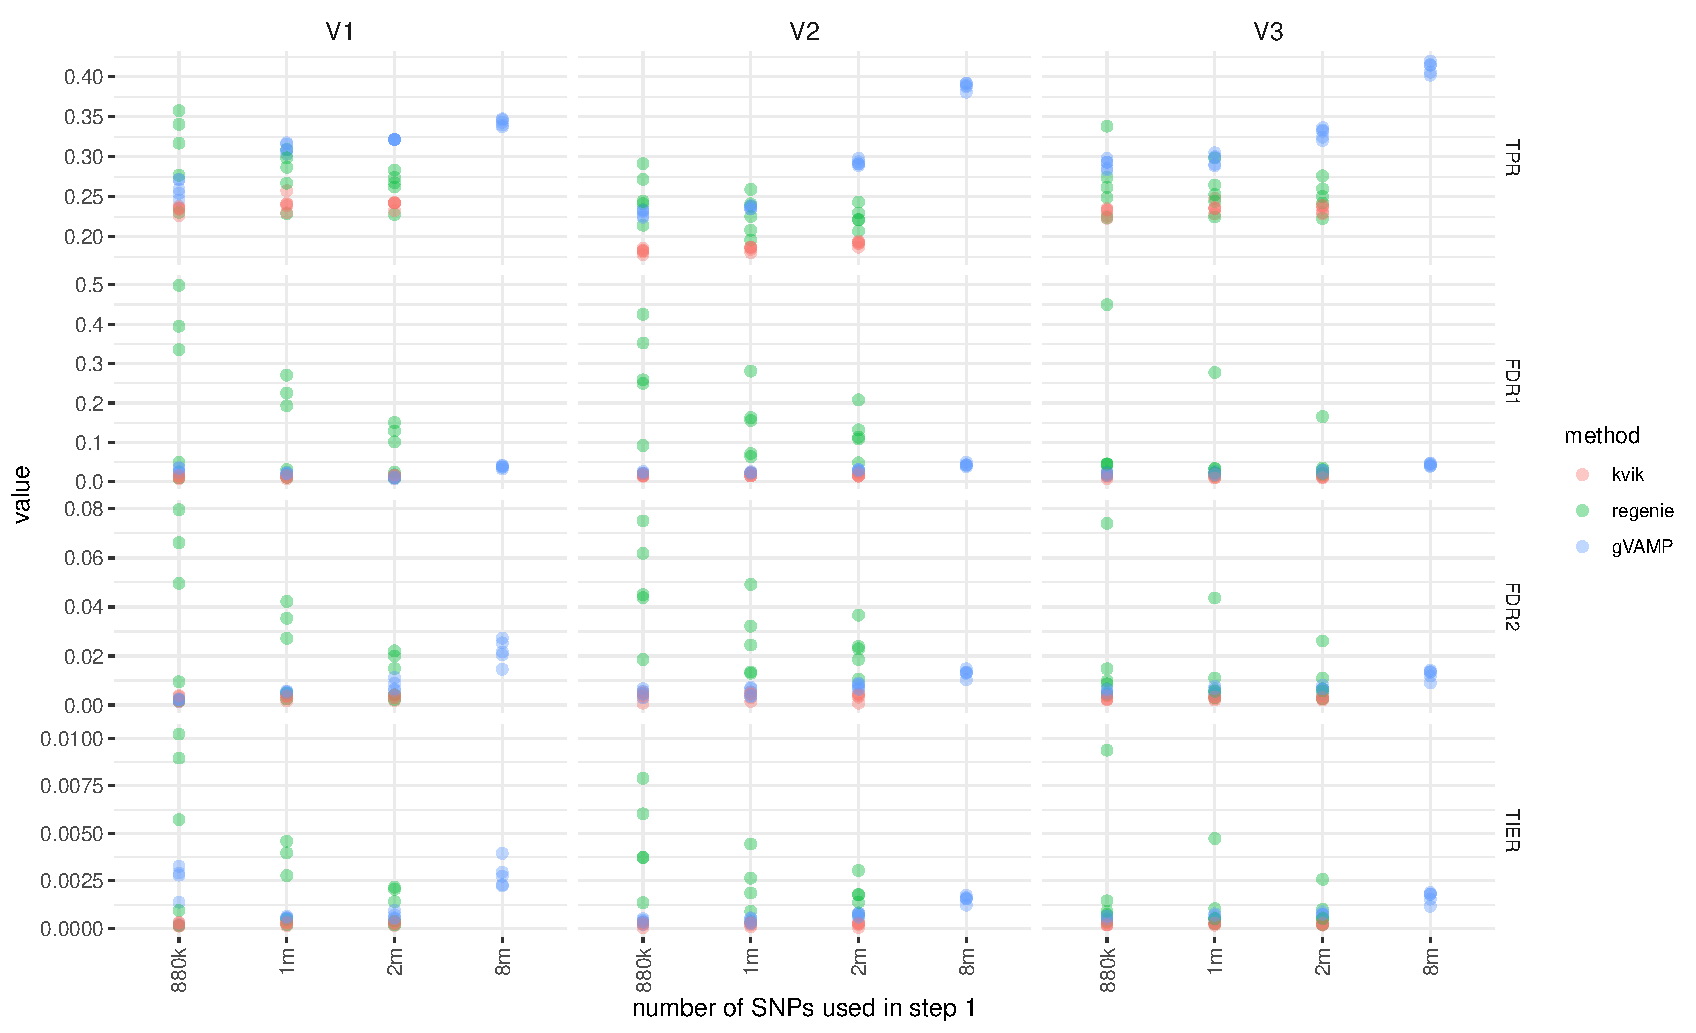
\includegraphics[width=\linewidth]{graphics/gVAMP_figures/Fig_SN3.pdf}
    \caption[Simulation study of true positive rate (TPR), false discovery rate (FDR) and type-I error for mixed linear model leave-one-chromosome out association testing in UK Biobank imputed genotype data]{\textbf{Simulation study of true positive rate (TPR), false discovery rate (FDR) and type-I error for mixed linear model leave-one-chromosome out association testing in UK Biobank imputed genotype data.} \small{We compare performance of leave-one-chromosome-out association testing (LOCO) when the first step LOCO predictors are created at different sets of markers ("880k" = 887,060, "1m" = 1,410,525, "2m" = 2,174,071 SNPs) from gVAMP (blue), an elastic net model implemented in the LDAK software (red), and Regenie (green). Comparisons are made across three settings: "V1" where 40,000 causal variants are randomly selected from 8,430,446 SNP markers and effects are drawn from a Gaussian, "V2" where 40,000 causal variants are randomly selected from 8,430,446 SNP markers, with effects that have a power relationship to the minor allele frequency of -0.5, and "V3" where 40,000 causal variants are randomly selected from 8,430,446 SNP markers, with effects drawn from an elastic net distribution. For each 1Mb window that contains an identified genome-wide significant association, we then ask if the identified variants are correlated (squared correlation $\geq 0.01$) to a causal variant: if so, we classify the window as a true positive; otherwise, we classify it as a false positive. The true positive rate is calculated as the number of true positive 1Mb windows divided by the total number of simulated causal variants, and it is also known as the recall, or sensitivity, reflecting the power of a statistical test.}}
    \label{fig:figSN3}
\end{figure}

\begin{figure}[!t] % the continued legend, at the top of the page after the figure
    \ContinuedFloat
    \captionsetup{labelformat=continued}
    \caption[]{\small{We provide two measures of the false discovery rate: FDR1 is calculated as the number of false positive 1Mb windows divided by the number of 1Mb windows that contain genome-wide significant associations, and it is a measure of the proportion of independent discoveries that are false. FDR2 is calculated as the total number of false positive SNPs (squared correlation $\leq 0.01$ with a causal variant) identified divided by the total number of identified genome-wide significant associations. We calculate the type-I error rate (TIER) as the number of SNPs with no correlation to a causal variant (squared correlation $\leq 0.01$ with a causal variant) that pass the Bonferroni genome-wide significance testing threshold divided by the total number of SNPs that have no correlation to a causal variant (squared correlation $\leq 0.01$ with a causal variant).}}
\end{figure}

\begin{figure}[!htp]
    \centering   
    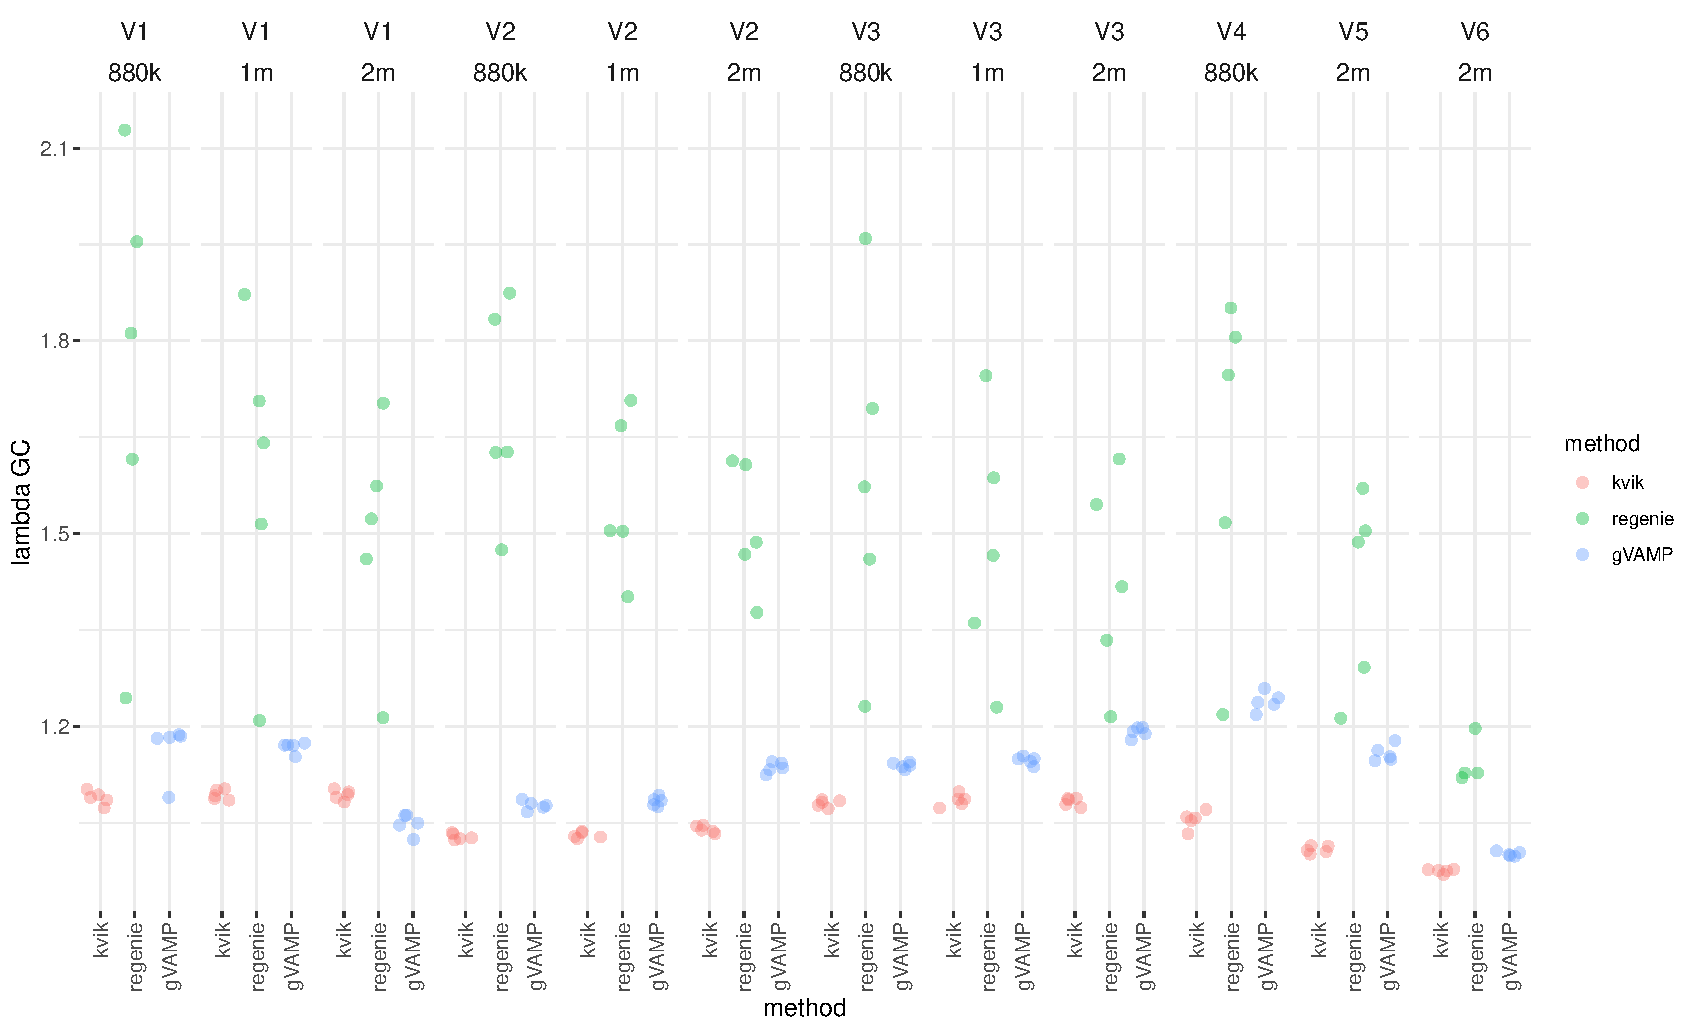
\includegraphics[width=\linewidth]{graphics/gVAMP_figures/Fig_SN7.pdf}
    \caption[Simulation study of lambda GC ($\lambda_{GC}$) values of mixed linear model leave-one-chromosome out association testing in UK Biobank imputed genotype data]{\textbf{Simulation study of lambda GC ($\lambda_{GC}$) values of mixed linear model leave-one-chromosome out association testing in UK Biobank imputed genotype data.} \small{We compare performance of leave-one-chromosome-out association testing (LOCO) when the first step LOCO predictors are created at different sets of markers, from gVAMP (blue), an elastic net model implemented in the LDAK software (red), and Regenie (green). Comparisons are made across six settings: "V1" where 40,000 causal variants are randomly selected from 8,430,446 SNP markers and effects are drawn from a Gaussian, "V2" where 40,000 causal variants are randomly selected from 8,430,446 SNP markers, with effects that have a power relationship to the minor allele frequency of -0.5, "V3" where 40,000 causal variants are randomly selected from 8,430,446 SNP markers, with effects drawn from an elastic net distribution, "V4" where 40,000 causal variants are randomly selected from 887,060 SNPs, with effects that contribute 50\% to the phenotypic variance and have a power relationship to the minor allele frequency of -0.5, "V5" where 40,000 causal variants are randomly selected from 2,174,071 SNPs, with effects that contribute 50\% to the phenotypic variance and have a power relationship to the minor allele frequency of -0.5, and "V6" where 5,000 causal variant effects are randomly selected from 2,174,071 SNPs, with effects that contribute 25\% to the phenotypic variance and have a power relationship to the minor allele frequency of -0.5. For each replicate, we calculate the ratio of the median chi-square to the expected median chi-square values ($\lambda_{GC}$).}}
    \label{fig:figSN4}
\end{figure}


\begin{figure}[!htp]
    \centering   
    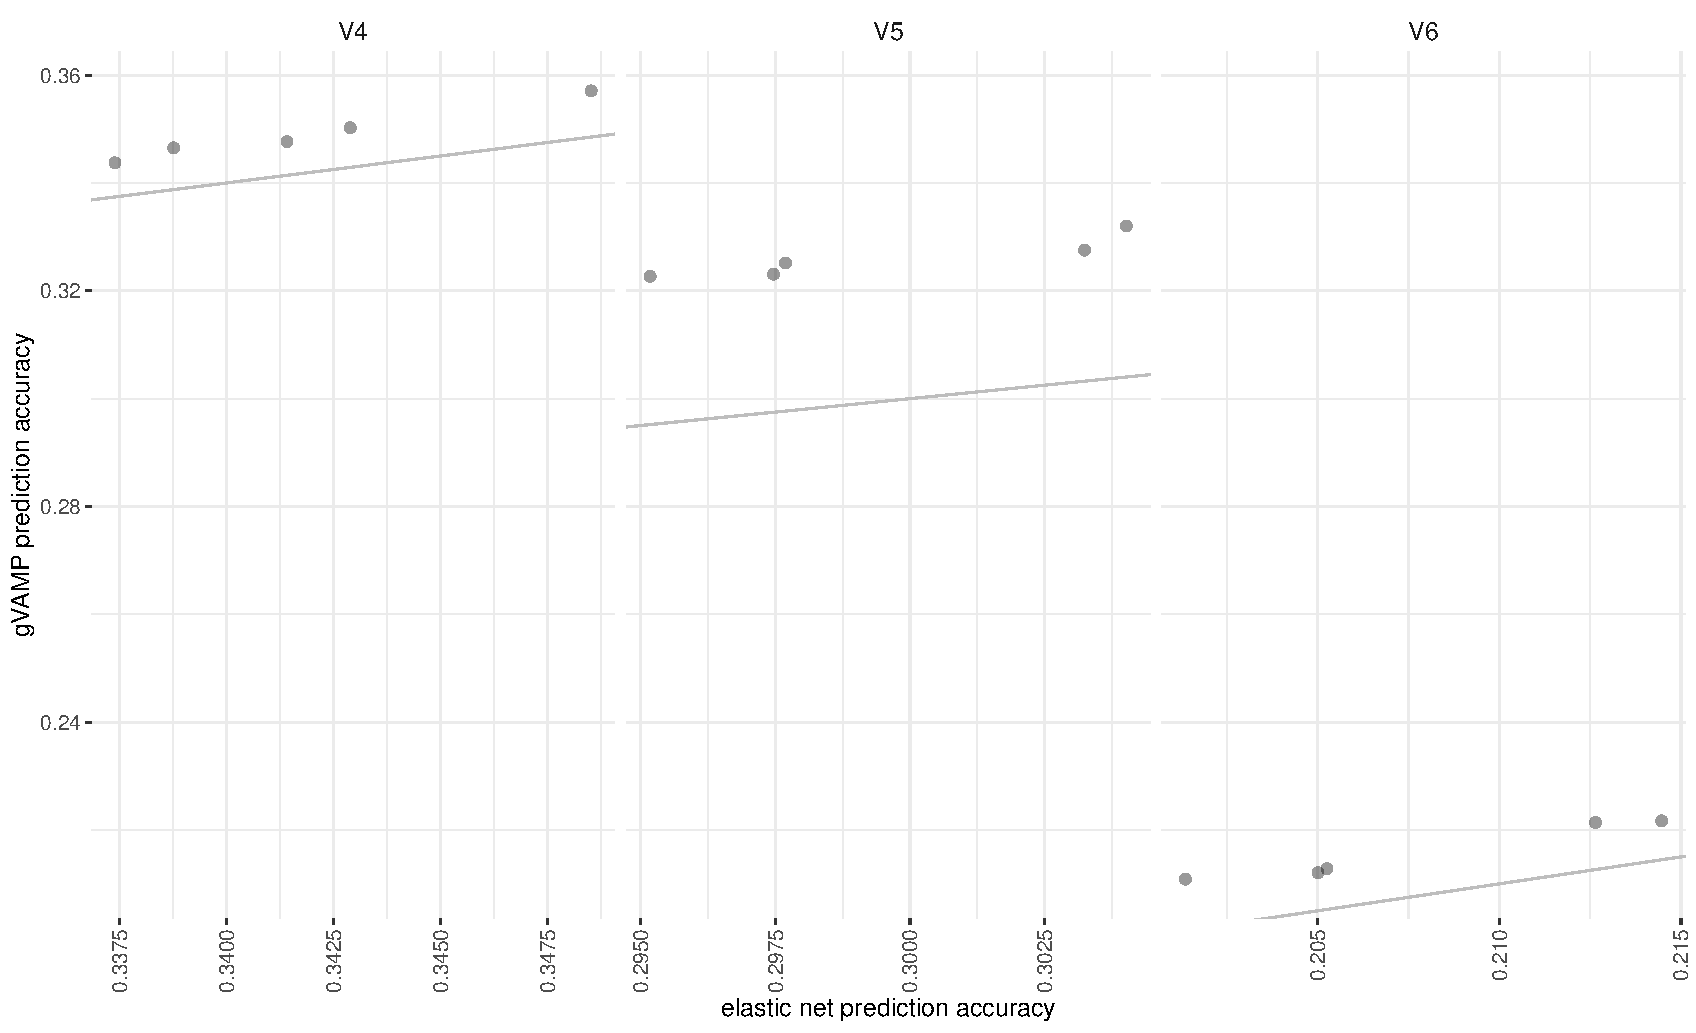
\includegraphics[width=\linewidth]{graphics/gVAMP_figures/Fig_SN4.pdf}
    \caption[Simulation study of out-of-sample prediction accuracy in UK Biobank imputed genotype data]{\textbf{Simulation study of out-of-sample prediction accuracy in UK Biobank imputed genotype data.} \small{We compare out-of-sample prediction accuracy ($y$-axis) for polygenic risk scores (PRS) created at different sets of markers from gVAMP and an elastic net model implemented in the LDAK software. Grey lines give the 1:1 line. Comparisons are made across three settings: "V4" where 40,000 causal variants are randomly selected from 887,060 SNPs, with effects that contribute 50\% to the phenotypic variance and have a power relationship to the minor allele frequency of -0.5, "V5" where 40,000 causal variants are randomly selected from 2,174,071 SNPs, with effects that contribute 50\% to the phenotypic variance and have a power relationship to the minor allele frequency of -0.5, and "V6" where 5,000 causal variant effects are randomly selected from 2,174,071 SNPs, with effects that contribute 25\% to the phenotypic variance and have a power relationship to the minor allele frequency of -0.5.}}
    \label{fig:figSN5}
\end{figure}

\begin{figure}[!htp]
    \centering   
    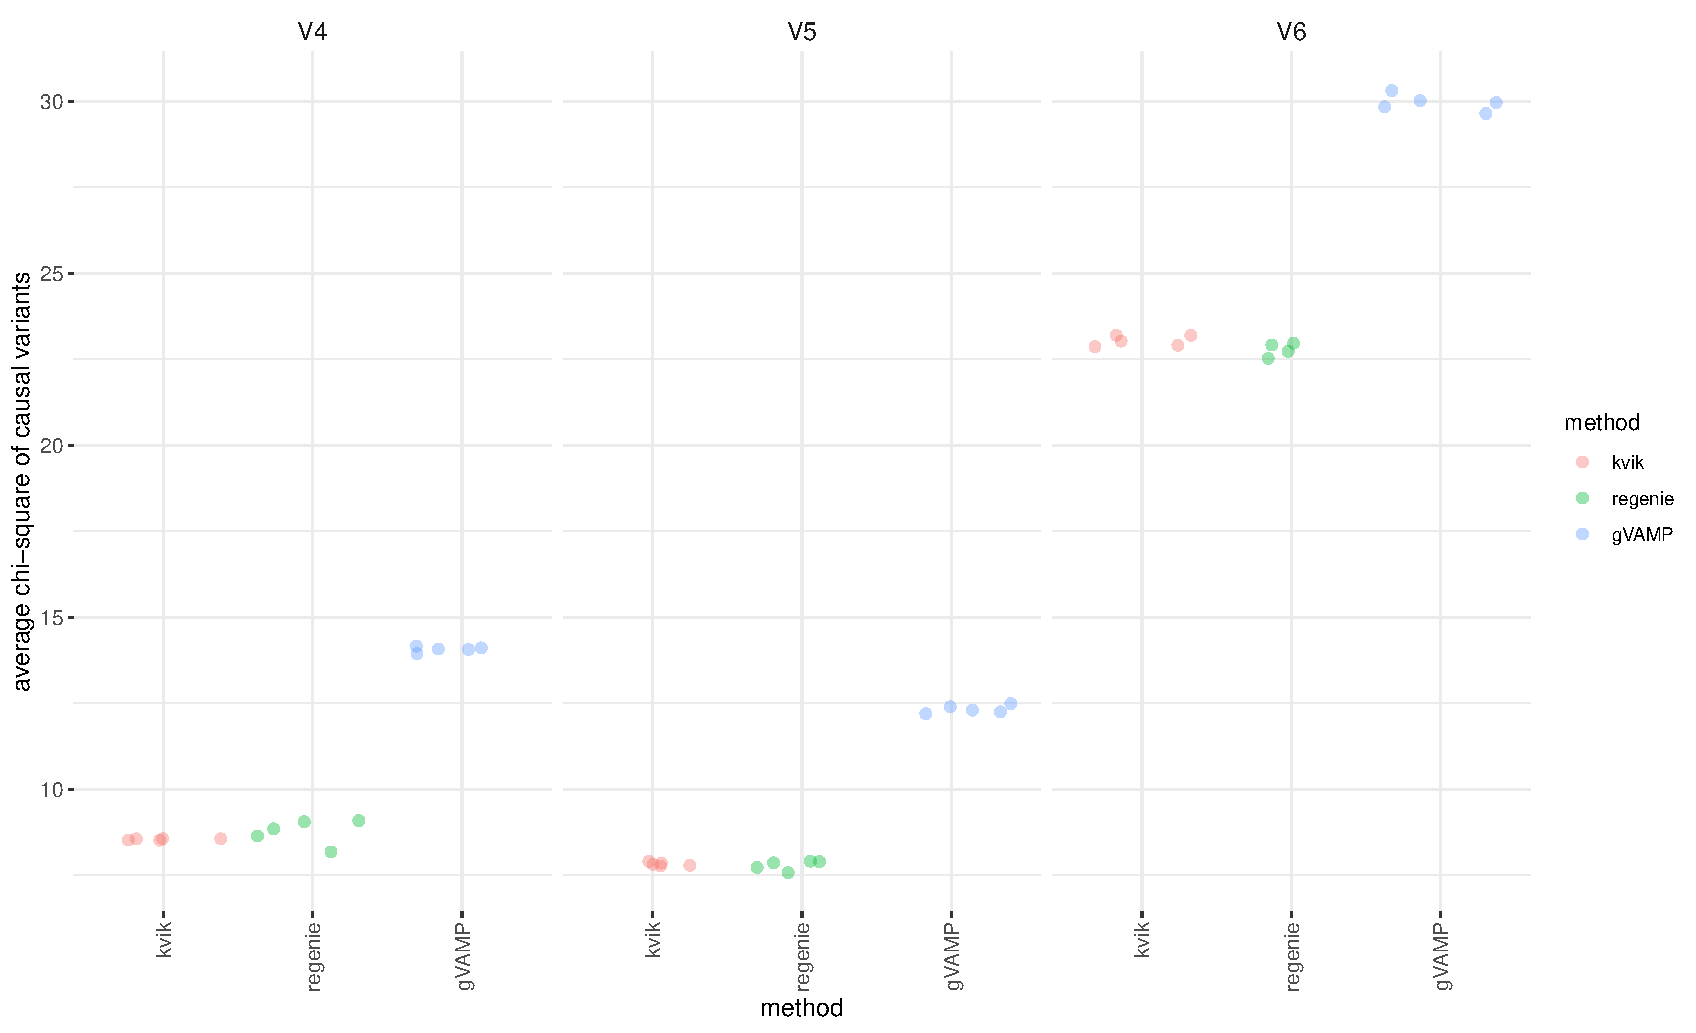
\includegraphics[width=\linewidth]{graphics/gVAMP_figures/Fig_SN5.pdf}
    \caption[Simulation study of power for mixed linear model leave-one-chromosome out association testing in UK Biobank imputed genotype data]{\textbf{Simulation study of power for mixed linear model leave-one-chromosome out association testing in UK Biobank imputed genotype data.} \small{We compare the average chi-squared value at the causal variants ($y$-axis) for leave-one-chromosome-out association testing (LOCO) when the first step LOCO predictors are created at different sets of markers, from gVAMP (blue), an elastic net model implemented in the LDAK software (red), and Regenie (green). Comparisons are made across three settings: "V4" where 40,000 causal variants are randomly selected from 887,060 SNPs, with effects that contribute 50\% to the phenotypic variance and have a power relationship to the minor allele frequency of -0.5, "V5" where 40,000 causal variants are randomly selected from 2,174,071 SNPs, with effects that contribute 50\% to the phenotypic variance and have a power relationship to the minor allele frequency of -0.5, and "V6" where 5,000 causal variant effects are randomly selected from 2,174,071 SNPs, with effects that contribute 25\% to the phenotypic variance and have a power relationship to the minor allele frequency of -0.5.}}
    \label{fig:figSN6}
\end{figure}

\begin{figure}[!htp]
    \centering   
    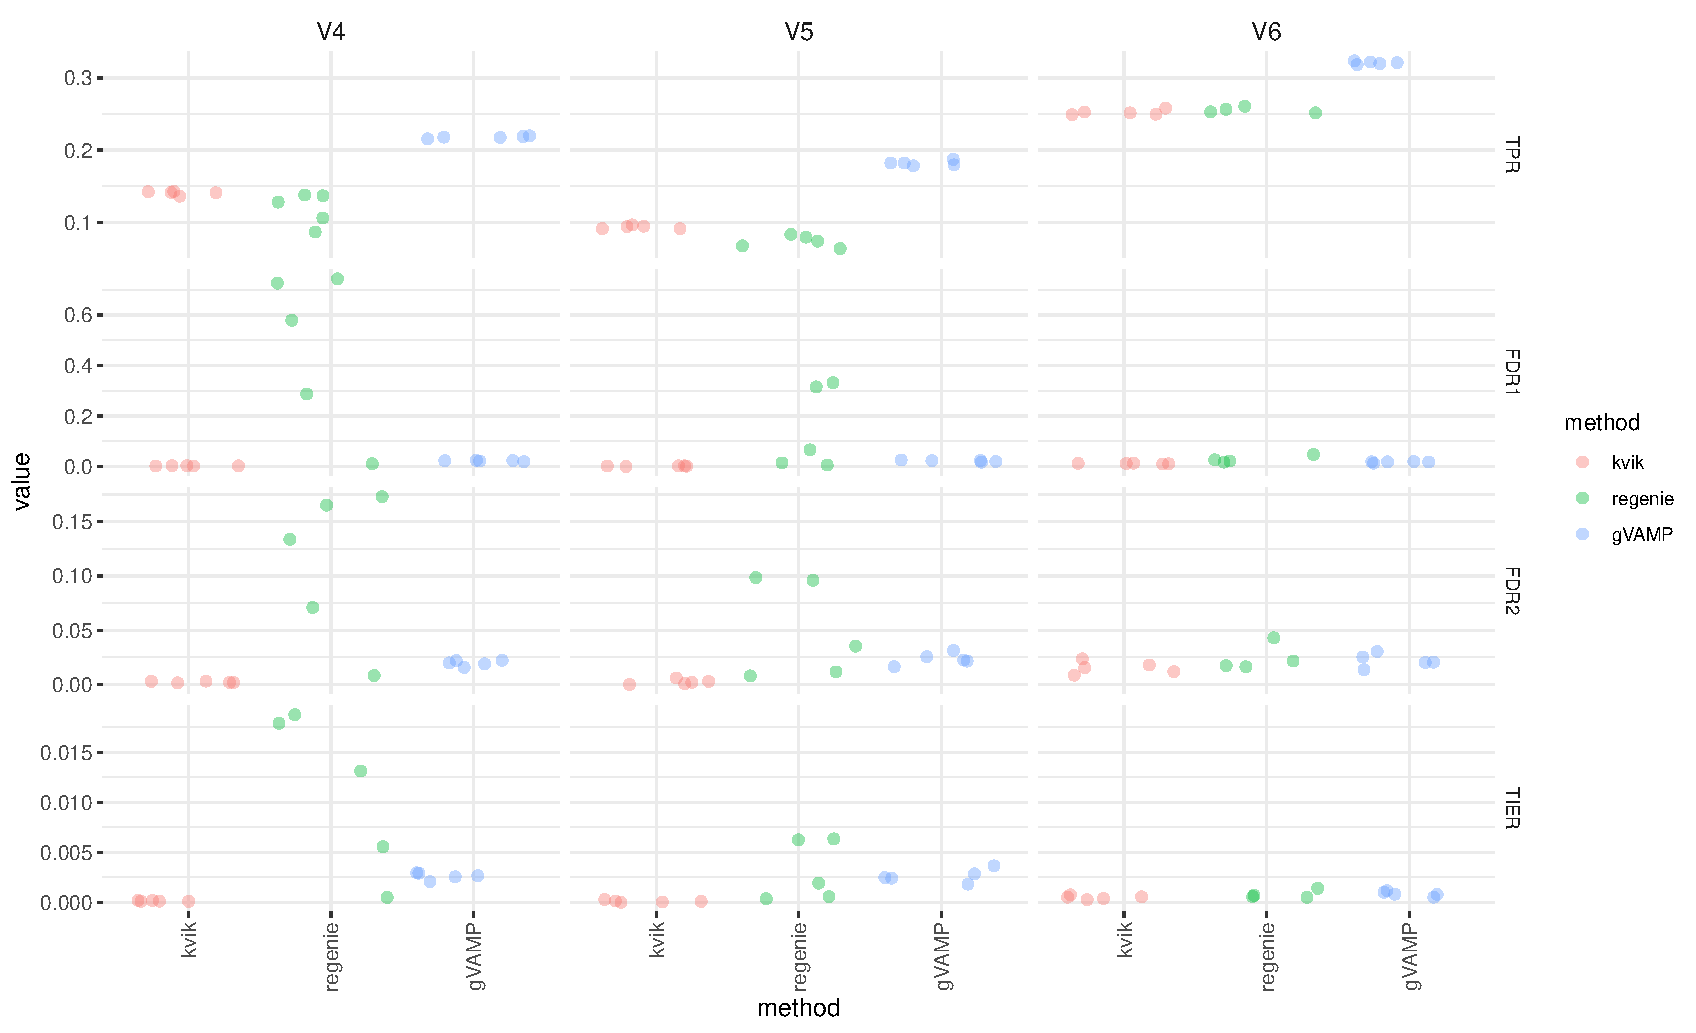
\includegraphics[width=\linewidth]{graphics/gVAMP_figures/Fig_SN6.pdf}
    \caption[Simulation study of true positive rate (TPR), false discovery rate (FDR) and type-I error for mixed linear model leave-one-chromosome out association testing in UK Biobank imputed genotype data]{\textbf{Simulation study of true positive rate (TPR), false discovery rate (FDR) and type-I error for mixed linear model leave-one-chromosome out association testing in UK Biobank imputed genotype data.} \small{We compare performance of leave-one-chromosome-out association testing (LOCO) when the first step LOCO predictors are created at different sets of markers, from gVAMP (blue), an elastic net model implemented in the LDAK software (red), and Regenie (green). Comparisons are made across three settings: "V4" where 40,000 causal variants are randomly selected from 887,060 SNPs, with effects that contribute 50\% to the phenotypic variance and have a power relationship to the minor allele frequency of -0.5, "V5" where 40,000 causal variants are randomly selected from 2,174,071 SNPs, with effects that contribute 50\% to the phenotypic variance and have a power relationship to the minor allele frequency of -0.5, and "V6" where 5,000 causal variant effects are randomly selected from 2,174,071 SNPs, with effects that contribute 25\% to the phenotypic variance and have a power relationship to the minor allele frequency of -0.5. For each 1Mb window that contains an identified genome-wide significant association, we then ask if the identified variants are correlated (squared correlation $\geq 0.01$) to a causal variant: if so, we classify the window as a true positive; otherwise, we classify it as a false positive. The true positive rate is calculated as the number of true positive 1Mb windows divided by the total number of simulated causal variants, and it is also known as the recall, or sensitivity, reflecting the power of a statistical test.}}
    \label{fig:figSN7}
\end{figure}

\begin{figure}[!t] % the continued legend, at the top of the page after the figure
    \ContinuedFloat
    \captionsetup{labelformat=continued}
    \caption[]{\small{We provide two measures of the false discovery rate: FDR1 is calculated as the number of false positive 1Mb windows divided by the number of 1Mb windows that contain genome-wide significant associations, and it is a measure of the proportion of independent discoveries that are false. FDR2 is calculated as the total number of false positive SNPs (squared correlation $\leq 0.01$ with a causal variant) identified divided by the total number of identified genome-wide significant associations. We calculate the type-I error rate (TIER) as the number of SNPs with no correlation to a causal variant (squared correlation $\leq 0.01$ with a causal variant) that pass the Bonferroni genome-wide significance testing threshold divided by the total number of SNPs that have no correlation to a causal variant (squared correlation $\leq 0.01$ with a causal variant).}}
\end{figure}


\begin{figure}[!htp]
    \centering
    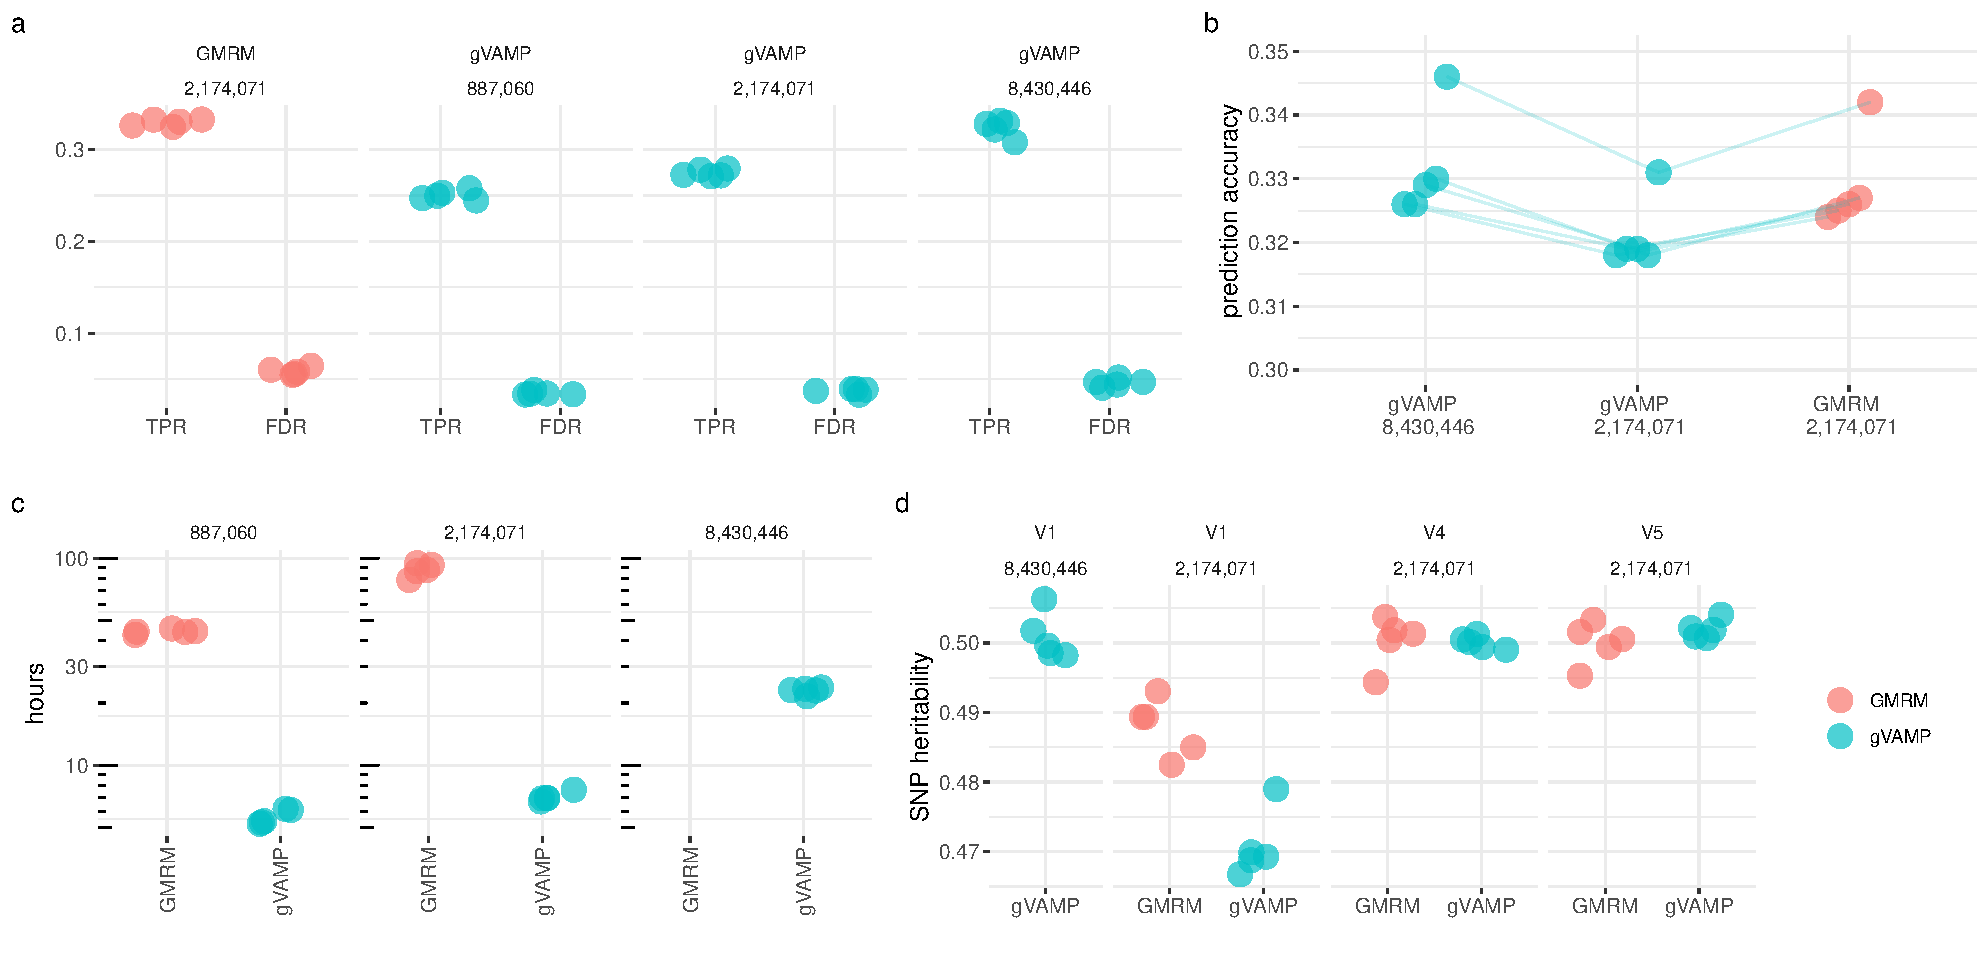
\includegraphics[width=\linewidth]{graphics/gVAMP_figures/gVAMP_GMRM.pdf}
    \caption[Comparison of MCMC Gibbs sampling algorithm GMRM to gVAMP in an imputed UK Biobank data simulation study]{\textbf{Comparison of MCMC Gibbs sampling algorithm GMRM to gVAMP in an imputed UK Biobank data simulation study.} \small For a simulation setting where 40,000 causal variants are randomly selected from 8,430,446 SNP markers and effects are drawn from a Gaussian ("V1"), in \emph{(a)}, we show results from standard leave-one-chromosome-out (LOCO) association testing where we select either all markers, 2,174,071 markers, or 887,060 markers for the first stage and then use all markers for the second stage LOCO testing. GMRM utilises 2,174,071 markers, whilst gVAMP can utilise the full range. We calculate the true positive rate (TPR) and the false discovery rate (FDR) and find that the FDR is well controlled at 5\% or less for both gVAMP and GMRM. For \emph{(b)}, we compare out-of-sample prediction accuracy for polygenic risk scores created at different sets of markers from gVAMP (8,430,446 and 2,174,071) and GMRM (2,174,071). \emph{(c)} gives the run time in hours for the first stage analysis of gVAMP and GMRM, across different marker sets using 50 CPU from a single compute node. \emph{(d)} gives a comparison of the proportion of phenotypic variation attributable to either 8,430,446 or a subset of 2,174,071 autosomal single nucleotide polymorphism (SNP) genetic markers (SNP heritability) estimated by GMRM and gVAMP. We consider three simulation scenarios: "V1" where 40,000 causal variants are randomly selected from 8,430,446 SNP markers and effects are drawn from a Gaussian, "V4" where 40,000 causal variants are randomly selected from 887,060 SNPs, with effects that contribute 50\% to the phenotypic variance and have a power relationship to the minor allele frequency of -0.5, "V5" where 40,000 causal variants are randomly selected from 2,174,071 SNPs, with effects that contribute 50\% to the phenotypic variance and have a power relationship to the minor allele frequency of -0.5. Points give the posterior means for GMRM and the convergence of gVAMP from five simulation replicates. Analysing 8,430,446 SNPs with gVAMP increases the heritability estimate over GMRM. This is consistent with an increase in phenotypic variance captured by the full imputed sequence data, as opposed to analyzing a selected subset of SNP markers, in which case gVAMP estimates are lower than those obtained from GMRM. Given the same data containing all the causal variants, the algorithms perform similarly irrespective of the underlying effect size distributions (``V4'' and ``V5'').}
    \label{fig:figSN8}
\end{figure}

\begin{figure}[!htp]
    \centering
    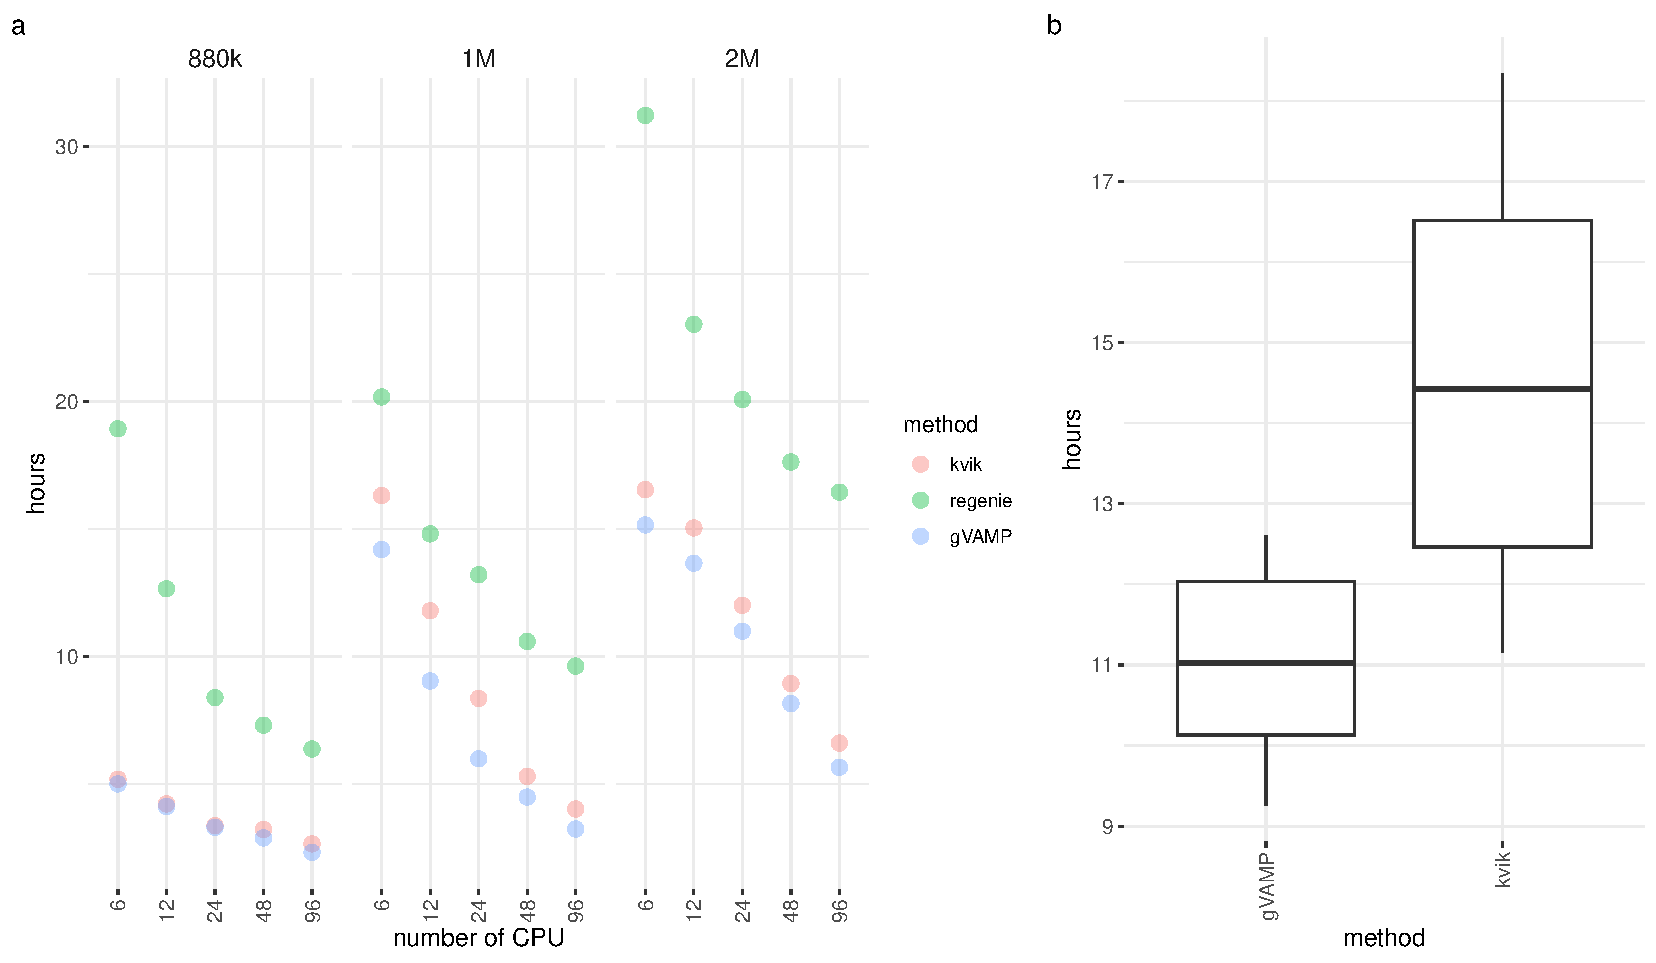
\includegraphics[width=\linewidth]{graphics/gVAMP_figures/timing_plot.pdf}
    \caption[Timing comparison of LDAK elastic net prediction model and gVAMP in an imputed UK Biobank data simulation study and across 13 UK Biobank traits]{\textbf{Timing comparison of LDAK elastic net prediction model and gVAMP in (a) an imputed UK Biobank data simulation study and (b) across 13 UK Biobank traits.} \small \emph{(a)} For simulation setting "V3" where 40,000 causal variants are randomly selected from 8,430,446 SNP markers, with effects drawn from an elastic net distribution, we show the total run time of the algorithms when run on different numbers of imputed SNP markers and given different numbers of CPU resources from a single AMD EPYC 7763 (64 cores, 2.45 GHz base-frequency) compute machine. \emph{(b)} A boxplot of the run time of the algorithms when run on $13$ different UK Biobank traits and 2,174,071 SNPs, when given 60 CPU. Training data sample size is given in Table \ref{table:tableS2} for each trait.}
    \label{fig:figSN9}
\end{figure}

\subsection*{Simulation study in imputed SNP data}
To support our empirical analyses we also conduct a simulation study in imputed SNP data using the 8,430,446 UK Biobank genetic marker data with 414,055 individuals. Our WGS simulation focused on variable selection of exact SNP positions and thus to give power to select variables and to enable clear comparisons of fine-mapping methods (where the objective was the selection of a single variable out of a segment) we simulated only 500 or 1000 causal variables on chromosomes 11-15. Here, we sought to simulate the other extreme of a very highly polygenic genetic basis and thus we randomly sample 40,000 causal variants genome-wide (effectively 4 times the density of causal variants simulated in the WGS simulation). We then simulate three scenarios. First, in \emph{V1}, we allocate effect sizes from a Gaussian with mean zero and variance $0.5/40000$, where $0.5$ is the proportion of variance attributable to the SNP markers. Multiplying the simulated SNP effects by normalized values of the 40,000 causal markers, gives a vector of genetic values of length $N=414055$ with variance 0.5. To this we add a vector of noise, drawn from a Gaussian with mean zero and variance 0.5, to produce a response variable of length $N$, with zero mean and unit variance. Second, in \emph{V2}, we simulate an $\alpha$-power relationship between the causal variant effect size and the minor allele frequency of $\alpha = -0.5$ (see Methods). Third, in \emph{V3}, we simulate under an elastic net prior, where with probability 0.8 we sample effect sizes from a standard Gaussian, with probability 0.2 we sample from a double exponential distribution, and we then scale the effects vector so that multiplying them with normalized values of the 40,000 causal markers, gives a vector of genetic values of length $N=414055$ with variance 0.5.

We analyze the simulated response variable with gVAMP, using either 8,430,446, 2,174,071, 1,410,525 or 887,060 SNP markers with identical initialization to that described in the Methods for the empirical UK Biobank study. We also analyze the data with REGENIE using 2,174,071, 1,410,525 or 887,060 SNP markers for the first stage and 8,430,446 SNP markers for the second stage LOCO testing. We then repeat the analysis again with LDAK-KVIK using 2,174,071, 1,410,525 or 887,060 SNP markers for the first stage and 8,430,446 SNP markers for the second stage LOCO testing. This creates three simulation scenarios where the heritability and number of causal variants is fixed, but the effect size distributions vary. We note that because the 2,174,071, 1,410,525 or 887,060 SNP marker sets are LD reduced subsets of the larger 8,430,446 SNP markers, the simulated causal variants are in LD with markers used in step 1, but they may not be present within the data. This is in contrast to the simulations presented in the LDAK-KVIK\cite{hof2024ldak} and REGENIE\cite{regenie} papers, where the causal variants are always within the subset of SNPs used in the first stage of the analysis.

We begin by comparing the out-of-sample prediction accuracy obtained by each approach for the different marker sets, following the same procedures outlined in the Methods for the empirical UK Biobank analysis. Note that it is not possible to obtain SNP marker effects for the model used in REGENIE step 1 and so we approximate this with a ridge-regression model implemented in the LDAK software. For the out-of-sample prediction, we use a hold-out set of 15,000 individuals that are unrelated (SNP marker relatedness $<0.05$) to the training individuals. We present these results in Figure \ref{fig:figSN1}. 

We then compare the LOCO association testing results obtained by REGENIE, LDAK-KVIK, and gVAMP. We estimate the average chi-squared value at the causal variants and present these results in Figure \ref{fig:figSN2}. We give a simple, fair comparison of the true positive rate (TPR) and false discovery rate (FDR) across methods controlling for LD, where we calculate the number of independent associations (squared correlation $\leq 0.01$) identified by each approach that pass a Bonferroni genome-wide significance testing threshold of $0.05/8430446$ within 1Mb windows of the DNA. Specifically, for each 1Mb window that contains an identified genome-wide significant association, we then ask if it is correlated (squared correlation $\geq 0.01$) to a causal variant: if so, we classify it as a true positive; otherwise, we classify it as a false positive. The true positive rate is calculated as the number of true positive 1Mb windows divided by the total number of simulated causal variants, and it is also known as the recall, or sensitivity, reflecting the power of a statistical test. We provide two measures of the false discovery rate: FDR1 is calculated as the number of false positive 1Mb windows divided by the number of 1Mb windows that contain genome-wide significant associations, and it is a measure of the proportion of independent discoveries that are false. FDR2 is calculated as the total number of false positive SNPs (squared correlation $\leq 0.01$ with a causal variant) identified divided by the total number of identified genome-wide significant associations. As genome-wide association studies aim to detect regions of the DNA associated with the phenotype, the definition of a false discovery as the detection of a variant at genome-wide significance when that variant has squared correlation $\leq 0.01$ with a causal variant within 1Mb is a very conservative one. Additionally, we calculate the type-I error rate as the number of SNPs with no correlation to a causal variant (squared correlation $\leq 0.01$ with a causal variant) that pass the Bonferroni genome-wide significance testing threshold divided by the total number of SNPs that have no correlation to a causal variant (squared correlation $\leq 0.01$ with a causal variant). We present these results in Figure \ref{fig:figSN3}. Finally, we also calculate the ratio of the median chi-square to the expected median chi-square values ($\lambda_{GC}$) and we present these results in Figure \ref{fig:figSN4}. We conduct five simulation replicates for each simulation scenarios, as we find that this is more than sufficient to contrast methods, as the results were very consistent across replicates. 

We then further conduct another three simulation scenarios: \emph{V4} where the 40,000 causal variants are drawn from the 2,174,071 SNP subset and we simulate a $\alpha$-power relationship between the causal variant effect size and the minor allele frequency of $\alpha = -0.5$; \emph{V5} where the 40,000 causal variants are drawn from the 887,060 SNP subset and we simulate a $\alpha$-power relationship between the causal variant effect size and the minor allele frequency of $\alpha = -0.5$; and \emph{V6} where the 5,000 causal variants are drawn from the 2,174,071 SNP subset with SNP-heritability = 0.25 and we simulate a $\alpha$-power relationship between the causal variant effect size and the minor allele frequency of $\alpha = -0.5$. Here, our objective in \emph{V4}, \emph{V5}, and \emph{V6} is to compare REGENIE, LDAK-KVIK and gVAMP in the scenario where the causal variants are present in the data used to create the predictors for the first step of LOCO as to date simulations for these methods have assumed this. This ensures that our findings are not just driven by only having SNPs correlated with the causal variants in step 1. We present these results, comparing prediction accuracy of LDAK to gVAMP in Figure \ref{fig:figSN5}, comparing the chi-squared values at the causal variants from REGENIE, LDAK, and gVAMP in Figure \ref{fig:figSN6}, and comparing the TPR and FDR of REGENIE, LDAK, and gVAMP in Figure \ref{fig:figSN7}. 

Additionally, we compare to GMRM using 2,174,071 SNP markers (as this completes within reasonable compute time and resource use), running for 2,500 iterations with 500 iteration burn in. Our objective is to compare GMRM and gVAMP to empirically assess the Bayes optimality of gVAMP when applied to genomic data. We compare the LOCO association testing, the out-of-sample prediction accuracy, the run time, and the SNP heritability of the two methods under the scenarios "V1", "V4" and "V5". We present these results in Figure \ref{fig:figSN8}. Finally, we compare the run time of REGENIE, LDAK and gVAMP both in a controlled simulation setting "V3" and across the 13 UK Biobank traits. We present these results in Figure \ref{fig:figSN9}.

\subsection*{Imputed data simulation study results}

For mixed linear model association testing (MLMA), association testing power (TPR) depends upon the sample size and the out-of-sample prediction accuracy of the predictors obtained from the first step~\cite{mlma}. Polygenic risk score prediction accuracy depends upon $h^{2}_{SNP}$, the number of true underlying causal variants and the sample size~\cite{daetwyler}, which are fixed in our simulation allowing a comparison of prediction accuracy obtained by different approaches across different genetic architectures. We find that prediction accuracy increases as marker number increases for all approaches (Figure \ref{fig:figSN1}). The prediction accuracy obtained by gVAMP is always slightly higher than that obtained by the LDAK model in every scenario and this difference becomes larger as more markers are used (Figure \ref{fig:figSN1}).

When these predictors are used for leave-one-chromosome-out MLMA testing, we find that the average chi-square values of the causal variants increases as marker number increases only for gVAMP (Figure \ref{fig:figSN2}). The values obtained by gVAMP are always higher than those obtained by LDAK or REGENIE and this difference becomes larger as more markers are used (Figure \ref{fig:figSN2}). We find that gVAMP has better LOCO association testing performance as compared to REGENIE or LDAK in terms of the TPR and FDR (Figure \ref{fig:figSN3}). In the simulation settings presented here, REGENIE does not control the FDR unless larger numbers of markers are used in step 1 (Figure \ref{fig:figSN3}). LDAK controls the FDR and type-I error well, comparative to gVAMP, but has lower TPR (Figure \ref{fig:figSN3}). gVAMP with larger numbers of SNPs used for step 1 gives higher TPR, whilst controlling the FDR below 5\% (Figure \ref{fig:figSN3}). Across all simulation settings, we find that the median chi-square value obtained from an MLMA-LOCO analysis with gVAMP is well controlled, showing the moderate elevation expected under polygenicity (Figure \ref{fig:figSN4}). This is in sharp contrast to REGENIE, which is elevated in all settings (Figure \ref{fig:figSN4}). The values obtained by LDAK rely on their proposal for adjusting the chi-square statistics and were generally lower than those obtained by MLMA-LOCO with gVAMP (Figure \ref{fig:figSN4}), even if we use the gVAMP LOCO predictors in place of the LDAK-KVIK ones and using LDAK-KVIK's proposed step 2 (Table \ref{table:tableS3}).

Similar patterns are also observed in the scenarios where the causal variants are present in the data used to create the predictors for the first step of LOCO, where gVAMP shows improved prediction accuracy (Figure \ref{fig:figSN5}), higher average-chi square values of the causal variants (Figure \ref{fig:figSN6}), higher TPR with controlled FDR (Figure \ref{fig:figSN7}). 

Finally, we also show that gVAMP has comparative performance to a similar MCMC implementation of a Bayesian mixture of Gaussians variable selection regression model (Figure \ref{fig:figSN8}). Analysing 8,430,446 SNPs with gVAMP increases the SNP-heritability estimate over GMRM. This is consistent with an increase in phenotypic variance captured by the full imputed sequence data, as opposed to analyzing a selected subset of SNP markers, in which case gVAMP estimates are lower than those obtained from GMRM (Figure \ref{fig:figSN8}). Given the same data containing all the causal variants, the algorithms perform similarly irrespective of the scenario (Figure \ref{fig:figSN8}).

\newpage

\refstepcounter{suppnotegvamp}
% \section{Supplementary Note \thesuppnotegvamp}
\section{Numerically stable calculation of the Onsager correction}
\label{supp:note2}
% \section*{Supplementary Note 2}
% \subsection*{Onsager correction calculation}
In order to ensure Gaussianity of residuals, gVAMP calculates the so-called Onsager correction based on \eqref{den_onsager}. For such calculation, the derivative of the denoising function $f_t$ defined in \eqref{denoiser_def} is required. Let us denote the numerator and denominator of \eqref{denoiser} with $\text{Num}(r_1)$ and $\text{Den}(r_1)$, respectively. Then, 
\begin{align}
    \begin{split}
    \frac{\partial \text{Num}(r_1)}{\partial r_1} & = \lambda_t \cdot \sum_{l=1}^L \pi_{t,l} \cdot \frac{\sigma_{t,l}^2}{(\gamma_{1,t}^{-1}+\sigma_{t,l}^2)^{3/2}} \cdot \text{EXP}(\sigma_{t,l}^2) \\
    & \quad \cdot \bigg [1 - r_1^2 \cdot \frac{(\sigma_{t,*}^2 - \sigma_{t,l}^2)}{(\gamma_{1,t}^{-1} + \sigma_{t,l}^2)(\gamma_{1,t}^{-1}+ \sigma_{t,*}^2)} \bigg ],
    \end{split}
\end{align}
\begin{equation}
    \begin{split}
    \frac{\partial \text{Den}(r_1)}{\partial r_1} & = -r_1 \cdot \bigg [ \lambda_t \cdot \sum_{l=1}^L \frac{\pi_{t,l}}{(\gamma_{1,t}^{-1} + \sigma_{t,l}^2)^{1/2}} \\
    & \qquad \cdot \frac{\sigma_{t,*}^2 - \sigma_{t,l}^2}{(\gamma_{1,t}^{-1} + \sigma_{t,l}^2)(\gamma_{1,t}^{-1}+\sigma_{t,*}^2)} \cdot \text{EXP}(\sigma_{t,l}^2) \\
    & \qquad +  (1 - \lambda_t) \cdot \frac{\gamma_{1,t}^{3/2} \cdot \sigma_{t, *}^2}{(\gamma_{1,t}^{-1}+\sigma_{t,*}^2)} \cdot \text{EXP}(0)  \bigg ].
    \end{split}
\end{equation}
Thus, the Onsager correction reads
\begin{align}
    \frac{\partial }{\partial r_1} \bigg ( \frac{\text{Num}(r_1)}{\text{Den}(r_1)} \bigg ) =  \frac{\frac{\partial}{\partial r_1} \text{Num}(r_1)}{\text{Den}(r_1)} - \frac{ \text{Num}(r_1) \cdot \frac{\partial}{\partial r_1}\text{Den}(r_1)}{(\text{Den}(r_1))^2}.
\end{align}
\vspace{5mm}

\newpage

\section{Conjugate gradient algorithm for solving linear systems}
\label{supp:note4}
\begin{breakablealgorithm}{Conjugate Gradient Method for Solving a Symmetric Linear System}{Conjugate gradient method for solving a symmetric linear system $\bm{Ax}=\bm{b}$.}{CG}
    
\begin{algorithmic}[1]
        \STATE {\bfseries Input:} Initial estimate of the solution $\bm{x}_0$, initial residual $\bm{r}_0=\bm{b}$, initial search direction $\bm{p}_0 = \bm{r}_0$, linear system matrix $\bm{A}$, right-hand side vector $\bm{b}$, stopping error threshold $\varepsilon >0$.
        \FOR{$n = 1,2,3,\dots$}
            \STATE $\alpha_n = \frac{\bm r_{n-1}^\top \bm r_{n-1}}{\bm p_{n-1}^\top\bm A \bm p_{n-1}}$ 
            \STATE $\bm x_n = \bm x_{n-1} + \alpha_n \bm p_{n-1}$ 
            \STATE $\bm r_n = \bm r_{n-1} - \alpha_n \bm A \bm p_{n-1}$ 
            \STATE $\beta_n = \frac{\bm r_n^\top \bm r_n}{\bm r_{n-1}^\top \bm r_{n-1}}$ 
            \STATE $\bm p_n = \bm r_n + \beta_n \bm p_{n-1}$ 
            \STATE \textbf{If} $n \ge 1$ and $||\bm{x}_n - \bm{x}_{n-1}||_2 / ||\bm{x}_n||_2 < \varepsilon$, then \textbf{break}
        \ENDFOR
        \STATE {\bfseries return} $\bm{x}_n$ 
\end{algorithmic}
\end{breakablealgorithm}

\newpage

\refstepcounter{suppnotegvamp}
% \section{Supplementary Note \thesuppnotegvamp}
\section{Multi-cohort denoiser and Onsager correction derivation}
\label{supp:note3}

We assume that a distribution on $\bm{\beta}$ follows spike and slab prior distribution, which is a mixture of a point mass at zero and a mixture of Gaussians:
\begin{align}
    \beta_j \sim (1-\lambda) \cdot \delta_0(\cdot) + \lambda \sum_{l=1}^L w_l \cdot \mathcal{N}(\cdot, 0, \sigma_l^2), \quad j=1, \dots, P,
\end{align}
where $1-\lambda$ is the sparsity rate, $w_l$ and $\sigma_l^2$ are the mixture weights and variances of the Gaussian components, respectively. We denote with $\Theta$ the set of parameters of the prior distribution, i.e. $\Theta = \{\lambda, w_1, \dots, w_L, \sigma_1^2, \dots, \sigma_L^2\}$.

In the continuation of this section we derive formula for 
\begin{equation}
\label{new_denoiser}
\begin{split}
f(\textbf{r}_{1,t}^{(1)}, \dots, \textbf{r}_{1,t}^{(K)}) & = \mathbb{E}[\bm{\beta} | \bm{r}_{1,t}^{(1)} = \bm{\beta} + \mathcal{N}(0, (\gamma_{1,t}^{(1)})^{-1}\bm{I}), \dots, \\
& \qquad \bm{r}_{1,t}^{(K)} = \bm{\beta} + \mathcal{N}(0, (\gamma_{1,t}^{(K)})^{-1}\bm{I}), \Theta_{t}],
\end{split}
\end{equation}
where $\bm{r}_{1,t}^{(i)}$ and $\gamma_{1,t}^{(i)}$ denote values of objects $\bm{r}_{1,t}$ and $\gamma_{1,t}$ when the basic algorithm is run on the i-th subpopulation. Also, we assume that the prior distribution parameters $\Theta$ are known.

First, we recall a well-known fact about Gaussian distributions from \cite{bromiley_products_2013}: denote with $(N(\mu_i, \eta_i))_{i=1}^M$ a family of Gaussian PDFs with specified means and standard deviations. Here and below, a subscript $1{:}M$ marks a quantity that combines all indices $i=1,\dots,M$ (e.g., $\eta_{1:M}$). Then
\begin{align}
    \label{prod_gaussians_PDFs}
    \prod_{i=1}^M N(x;\mu_i, \eta_i) = \frac{S_{1:M}}{\sqrt{2 \pi \eta^2_{1:M}}} \cdot \exp \bigg [ - \frac{(x-\mu_{1:M})^2}{2 \eta_{1:M}^2}\bigg ],
\end{align}
where 
\begin{gather}
    \frac{1}{\eta^2_{1:M}} = \sum_{i=1}^M \frac{1}{\eta^2_i}, \qquad \mu_{1:M} = \eta^2_{1:M} \sum_{i=1}^M \frac{\mu_i}{\eta_i^2}, \qquad \text{and} \nonumber \\
    S_{1:M} = \frac{1}{(2\pi)^{(M-1)/2}} \sqrt{\frac{\eta^2_{1:M}}{\prod_{i=1}^M \eta_i^2}} \, \exp \bigg [ -\frac{1}{2} \bigg ( \sum_{i=1}^M \frac{\mu_i^2}{\eta_i^2} - \frac{\mu^2_{1:M}}{\eta^2_{1:M}} \bigg ) \bigg ].
\end{gather}

\subsection*{Constructing denoisers}
Note that acting of $(\ref{new_denoiser})$ is component-wise on the entries of $\bm{r}_{1,t}^{(1)}, \dots,\allowbreak \bm{r}_{1,t}^{(K)}$. %, which we for simplicity denote as $r_1, \dots, r_K$, can be rewritten as
\begin{equation}
    \label{step1}
    \begin{split}
    f(\textbf{r}_1^{(1)}, \dots, \textbf{r}_1^{(K)}) & = \frac{1}{Z} \cdot \int \beta \bigg [(1-\lambda) \cdot \delta_0(\beta) + \lambda \sum_{l=1}^L w_l \cdot N(\beta; 0, \sigma_l^2) \bigg ] \\
    & \qquad \cdot \prod_{i=1}^K N(\beta; \textbf{r}_1^{(i)}, 1/\gamma_{1}^{(i)} ) d \beta,
    \end{split}
\end{equation}
where 
\begin{align}
    \begin{split}
    Z & = \int \bigg [(1-\lambda) \cdot \delta_0(\beta) + \lambda \sum_{l=1}^L w_l \cdot N(\beta; 0, \sigma_l^2) \bigg ] \\
    & \qquad \cdot \prod_{i=1}^K N(\beta; \textbf{r}_1^{(i)}, 1/\gamma_{1}^{(i)} ) d \beta,
    \end{split}
\end{align}
is a normalization constant. We separate expression \eqref{step1} into several integrals each representing one of the mixture groups. To proceed from this for a group $l \in \{1, \dots, L\}$, we use the formula \eqref{prod_gaussians_PDFs} with $M=K+1, \mu_i = \textbf{r}_1^{(i)}, \forall i=1,\dots, K, \mu_{K+1} = 0$ and $\eta_i = \sqrt{1/\gamma_1^{(i)}}, \forall i=1, \dots, K$ and $\eta_{K+1} = \sigma_l$. Therefore, for $l \in \{1,\dots, L\}$, the integral 
\begin{equation}
    \frac{1}{Z} \cdot \int \beta \cdot \lambda \cdot  w_l \cdot N(\beta; 0, \sigma_l^2) \cdot \prod_{i=1}^K N(\beta; \textbf{r}_1^{(i)}, 1/\gamma_{1}^{(i)} ) d \beta
\end{equation}
can be re-written as 
\begin{align}
    \label{rewritting_expe_l}
    \begin{split}
    & \frac{1}{Z} \int \beta \cdot \frac{\lambda w_l S_{1:K+1}^{(l)}}{\sqrt{2 \pi (\eta_{1:K+1}^{(l)})^2}} \exp \bigg [ -\frac{(\beta - \mu_{1:K+1}^{(l)})^2}{2 (\eta_{1:K+1}^{(l)})^2} \bigg ] d \beta \\
    & \quad = \frac{\lambda w_l S_{1:K+1}^{(l)}}{Z} \int \beta \cdot \frac{1}{\sqrt{2 \pi (\eta_{1:K+1}^{(l)})^2}} \exp \bigg [ -\frac{(\beta - \mu_{1:K+1}^{(l)})^2}{2 (\eta_{1:K+1}^{(l)})^2} \bigg ] d \beta \\
    & \quad = \frac{\lambda w_l S_{1:K+1}^{(l)}}{Z} \int \beta \cdot \mathcal{N} \big( \beta; \mu_{1:K+1}^{(l)}, (\eta_{1:K+1}^{(l)})^2 \big) \, d \beta \\
    & \quad = \frac{1}{Z} \, \lambda w_l S_{1:K+1}^{(l)} \mu_{1:K+1}^{(l)},
    \end{split}
\end{align}
where 
\begin{multline}
    S_{1:K+1}^{(l)} := \frac{1}{(2\pi)^{K/2}} \sqrt{\frac{(\eta^{(l)}_{1:K+1})^2}{\sigma_l^2 \prod_{i=1}^K 1/\gamma_1^{(i)}}} \\
    \cdot \exp \bigg [ -\frac{1}{2} \bigg ( \sum_{i=1}^{K} \gamma_1^{(i)} (r_1^{(i)})^2 - \frac{(\mu^{(l)}_{1:K+1})^2}{(\eta^{(l)}_{1:K+1})^2} \bigg ) \bigg ].
\end{multline}
Furthermore, using the following property of delta functions: $\int f(x) \delta_0(x) dx = f(0)$ we get that:
\begin{align}
    \label{spike_part}
    \int \beta \cdot (1-\lambda) \cdot \delta_0(\beta) \cdot \prod_{i=1}^K N(\beta; \textbf{r}_1^{(i)}, 1/\gamma_{1}^{(i)} ) d \beta = 0.
\end{align}
Now, using \eqref{spike_part} and equality \eqref{rewritting_expe_l} for $l=1,\dots, L$, we can rewrite \eqref{new_denoiser} as
\begin{align}
    \label{step_final}
     f(\textbf{r}_1^{(1)}, \dots, \textbf{r}_1^{(K)}) = \frac{1}{Z} \cdot \lambda \cdot \sum_{l=1}^L w_l \cdot S_{1:K+1}^{(l)}\cdot \mu_{1:K+1}^{(l)}.
    % \frac{1}{Z} \cdot \bar{S} \cdot \bar{\mu} \cdot \lambda,
\end{align}
What remains is to find a closed-form expression for $Z$. Again using the following property of delta functions: $\int f(x) \delta_0(x) dx = f(0)$ and equality (\ref{prod_gaussians_PDFs}) we get
\begin{align}
    \label{constZ}
    \begin{split}
    Z & = \int \bigg[ (1-\lambda) \, \delta_0(\beta) + \lambda \sum_{l=1}^L w_l N(\beta; 0, \sigma_l^2) \bigg] \prod_{i=1}^K N(\beta; \textbf{r}_1^{(i)}, 1/\gamma_{1}^{(i)}) \, d \beta \\
    & = (1-\lambda) \prod_{i=1}^K N(0; \textbf{r}_1^{(i)}, 1/\gamma_{1}^{(i)}) \\
    & \qquad + \sum_{l=1}^L \int \frac{\lambda w_l S_{1:K+1}^{(l)}}{\sqrt{2 \pi (\eta_{1:K+1}^{(l)})^2}} \exp \bigg[ -\frac{(\beta - \mu_{1:K+1}^{(l)})^2}{2 (\eta_{1:K+1}^{(l)})^2} \bigg] d \beta \\
    & = (1-\lambda) \prod_{i=1}^K N(0; \textbf{r}_1^{(i)}, 1/\gamma_{1}^{(i)}) + \lambda \sum_{l=1}^L w_l S_{1:K+1}^{(l)}.
    \end{split}
\end{align}

Finally, gathering \eqref{step_final} and the closed-form expression for $Z$, we get:
\begin{align}
    \label{final_den}
    \begin{split}
     & f(\textbf{r}_1^{(1)}, \dots, \textbf{r}_1^{(K)}) \\
     & = \frac{ \lambda \cdot \sum_{l=1}^L w_l \cdot S_{1:K+1}^{(l)}\cdot \mu_{1:K+1}^{(l)} }{ (1-\lambda) \cdot \prod_{i=1}^K N(0; \textbf{r}_1^{(i)}, 1/\gamma_{1}^{(i)} ) + \lambda \cdot \sum_{l=1}^L w_l \cdot S_{1:K+1}^{(l)} } \\
     & = \frac{ \lambda \cdot \sum_{l=1}^L w_l \cdot  \exp \bigg (\frac{1}{2} \cdot \frac{(\mu^{(l)}_{1:K+1})^2}{(\eta^{(l)}_{1:K+1})^2}  \bigg ) \cdot \mu_{1:K+1}^{(l)} \cdot \sqrt{(\eta^{(l)}_{1:K+1})^2 / \sigma_l^2} }{ (1-\lambda) + \lambda \cdot \sum_{l=1}^L w_l \cdot \exp \bigg (\frac{1}{2} \cdot \frac{(\mu^{(l)}_{1:K+1})^2}{(\eta^{(l)}_{1:K+1})^2}  \bigg ) \cdot \sqrt{(\eta^{(l)}_{1:K+1})^2 / \sigma_l^2} },
     \end{split}
\end{align}
where
\begin{align}
    (\eta^{(l)}_{1:K+1})^2 = \frac{1}{\sum_{i=1}^K \gamma_1^{(i)}+1/\sigma_l^2}, \quad \mu^{(l)}_{1:K+1} = \frac{\sum_{i=1}^K r_1^{(i)} \cdot \gamma_1^{(i)}}{\sum_{i=1}^K \gamma_1^{(i)}+1/\sigma_l^2}.
\end{align}
For reasons of numerical stability of the formula \eqref{final_den} we introduce

% \begin{align*}
%     * = \argmax_{l=1,\dots, L} \bigg \{ \frac{(\mu^{(l)}_{1:K})^2}{(\eta^{(l)}_{1:K})^2} \bigg \}
% \end{align*}
% and we evaluate the formula \eqref{final_den} as

% \resizebox{.7\linewidth}{!}{
%   \begin{minipage}{\linewidth}
% \begin{align}
%     \label{final_den_stable}
%     \begin{split}
%      f(\textbf{r}_1^{(1)}, \dots, \textbf{r}_1^{(K)}) & = \frac{ \lambda \cdot \sum_{l=1}^L w_l \cdot  \exp \bigg (\frac{1}{2} \cdot \frac{(\mu^{(l)}_{1:K+1})^2 \cdot (\eta^{(*)}_{1:K})^2 - (\mu^{(*)}_{1:K})^2 \cdot (\eta^{(l)}_{1:K})^2}{(\eta^{(l)}_{1:K+1})^2 \cdot (\eta^{(*)}_{1:K})^2}  \bigg ) \cdot \mu_{1:K+1}^{(l)} \cdot \sqrt{(\eta^{(l)}_{1:K+1})^2 / \sigma_l^2}}{ (1-\lambda) \cdot \exp \bigg (-\frac{1}{2} \cdot \frac{(\mu^{(*)}_{1:K+1})^2}{(\eta^{(*)}_{1:K+1})^2}  \bigg ) + \lambda \cdot \sum_{l=1}^L w_l \cdot \exp \bigg ( \frac{1}{2} \cdot \frac{(\mu^{(l)}_{1:K+1})^2 \cdot (\eta^{(*)}_{1:K})^2 - (\mu^{(*)}_{1:K})^2 \cdot (\eta^{(l)}_{1:K})^2}{(\eta^{(l)}_{1:K+1})^2 \cdot (\eta^{(*)}_{1:K})^2}  \bigg ) \cdot \sqrt{(\eta^{(l)}_{1:K+1})^2 / \sigma_l^2} }.
%      \end{split}
% \end{align}
%   \end{minipage}
% }

%%%%%%%%%%%%%%%
\begin{align}
    * &= \argmax_{l=1,\dots, L} \bigg \{ \frac{(\mu^{(l)}_{1:K})^2}{(\eta^{(l)}_{1:K})^2} \bigg \}
\end{align}
and we evaluate the formula \eqref{final_den} as

\begin{align}
    \label{final_den_stable}
    \begin{split}
    f(\textbf{r}_1^{(1)}, \dots, \textbf{r}_1^{(K)}) & = \Bigg\{ \lambda \sum_{l=1}^L w_l \, \mu_{1:K+1}^{(l)} \sqrt{(\eta^{(l)}_{1:K+1})^2 / \sigma_l^2} \\
    & \quad \times \exp \bigg( \frac{1}{2} \, \frac{(\mu^{(l)}_{1:K+1})^2 (\eta^{(*)}_{1:K})^2 - (\mu^{(*)}_{1:K})^2 (\eta^{(l)}_{1:K})^2}{(\eta^{(l)}_{1:K+1})^2 (\eta^{(*)}_{1:K})^2} \bigg) \Bigg\} \\
    & \quad \times \Bigg\{ (1-\lambda) \exp \bigg( -\frac{1}{2} \, \frac{(\mu^{(*)}_{1:K+1})^2}{(\eta^{(*)}_{1:K+1})^2} \bigg) \\
    & \qquad + \lambda \sum_{l=1}^L w_l \sqrt{(\eta^{(l)}_{1:K+1})^2 / \sigma_l^2} \\
    & \quad \times \exp \bigg( \frac{1}{2} \, \frac{(\mu^{(l)}_{1:K+1})^2 (\eta^{(*)}_{1:K})^2 - (\mu^{(*)}_{1:K})^2 (\eta^{(l)}_{1:K})^2}{(\eta^{(l)}_{1:K+1})^2 (\eta^{(*)}_{1:K})^2} \bigg) \Bigg\}^{-1}.
    \end{split}
\end{align}
%%%%%%%%%%%%%%%

\subsection*{Derivation of the Onsager correction}
If we denote the numerator and denominator from the expression \eqref{final_den_stable} with $\text{Num(f)}$ and $\text{Den}(f)$, then using the quotient rule for derivative we obtain that
\begin{align}
    \label{quotient_rule}
    \frac{\partial f}{\partial r_1^{(i)}} =\frac{\frac{\partial}{\partial r_1^{(i)}}\text{Num}(f) \cdot \text{Den}(f) - \frac{\partial}{\partial r_1^{(i)}}\text{Den}(f) \cdot \text{Num}(f)}{(\text{Den}(f))^2}. 
\end{align}

When evaluating formula \eqref{quotient_rule}, one can use the same numerical trick as in equation \eqref{final_den_stable} to make the computation more numerically stable.

% {
% \resizebox{0.95\linewidth}{!}{
%   \begin{minipage}{\linewidth}
% \begin{align*}
%     \frac{\partial}{\partial r_1^{(i)}} \text{Num}(f) & = \lambda \cdot \sum_{l=1}^L w_l \cdot (\mu^{(l)}_{1:K})^2 \cdot \exp \bigg ( \frac{1}{2} \cdot \frac{(\mu^{(l)}_{1:K+1})^2}{(\eta^{(l)}_{1:K+1})^2} \bigg ) \cdot \frac{1}{{(\eta^{(l)}_{1:K+1})^2}} \cdot \frac{\gamma_1^{(i)}}{\big ( \sum_{i=1}^K \gamma_1^{(i)}+1/\sigma_l^2 \big )} \cdot \sqrt{(\eta^{(l)}_{1:K+1})^2 / \sigma_l^2} \\ & \quad \quad \quad + \lambda \cdot \sum_{l=1}^L w_l \cdot \exp \bigg ( \frac{1}{2} \cdot \frac{(\mu^{(l)}_{1:K+1})^2}{(\eta^{(l)}_{1:K+1})^2} \bigg ) \cdot \frac{\gamma_1^{(i)}}{\sum_{i=1}^K \gamma_1^{(i)}+1/\sigma_l^2} \cdot \sqrt{(\eta^{(l)}_{1:K+1})^2 / \sigma_l^2} \\
%     & = \lambda \cdot \sum_{l=1}^L w_l \cdot \exp \bigg ( \frac{1}{2} \cdot \frac{(\mu^{(l)}_{1:K+1})^2}{(\eta^{(l)}_{1:K+1})^2} \bigg ) \cdot \bigg [  (\mu^{(l)}_{1:K})^2 + \frac{1}{\sum_{i=1}^K \gamma_1^{(i)}+1/\sigma_l^2} \bigg ] \cdot \gamma_1^{(i)} \cdot \sqrt{(\eta^{(l)}_{1:K+1})^2 / \sigma_l^2}
% \end{align*}
% \end{minipage}
% }
% }

% When evaluating formula (\ref{quotient_rule}), one can use the same numerical trick as in equation (\ref{final_den_stable}) to make the computation more numerically stable.

\begin{equation}
\begin{split}
    \frac{\partial}{\partial r_1^{(i)}} \text{Num}(f)
    & = \lambda \sum_{l=1}^L w_l \, (\mu^{(l)}_{1:K})^2 \exp \bigg( \frac{1}{2} \, \frac{(\mu^{(l)}_{1:K+1})^2}{(\eta^{(l)}_{1:K+1})^2} \bigg) \\
    & \qquad \times \frac{1}{(\eta^{(l)}_{1:K+1})^2} \, \frac{\gamma_1^{(i)}}{\sum_{i=1}^K \gamma_1^{(i)} + 1/\sigma_l^2} \, \sqrt{(\eta^{(l)}_{1:K+1})^2 / \sigma_l^2} \\
    & \quad + \lambda \sum_{l=1}^L w_l \exp \bigg( \frac{1}{2} \, \frac{(\mu^{(l)}_{1:K+1})^2}{(\eta^{(l)}_{1:K+1})^2} \bigg) \\
    & \qquad \times \frac{\gamma_1^{(i)}}{\sum_{i=1}^K \gamma_1^{(i)} + 1/\sigma_l^2} \, \sqrt{(\eta^{(l)}_{1:K+1})^2 / \sigma_l^2} \\
    & = \lambda \sum_{l=1}^L w_l \exp \bigg( \frac{1}{2} \, \frac{(\mu^{(l)}_{1:K+1})^2}{(\eta^{(l)}_{1:K+1})^2} \bigg) \\
    & \qquad \times \bigg[ (\mu^{(l)}_{1:K})^2 + \frac{1}{\sum_{i=1}^K \gamma_1^{(i)} + 1/\sigma_l^2} \bigg] \gamma_1^{(i)} \sqrt{(\eta^{(l)}_{1:K+1})^2 / \sigma_l^2}.
\end{split}
\end{equation}

\begin{equation}
    \frac{\partial}{\partial r_1^{(i)}} \text{Den}(f) = \lambda \sum_{l=1}^L w_l \, \mu^{(l)}_{1:K} \exp \bigg( \frac{1}{2} \, \frac{(\mu^{(l)}_{1:K+1})^2}{(\eta^{(l)}_{1:K+1})^2} \bigg) \, \gamma_1^{(i)} \sqrt{(\eta^{(l)}_{1:K+1})^2 / \sigma_l^2}.
\end{equation}

% \subsection{Case $K=1 \text{ } \& \text{ } L=1$}
% \begin{align*}
%     f(\textbf{r}_1) = \frac{\lambda \cdot \frac{\textbf{r}_1 \gamma_1 \sigma^2 }{(\gamma_1 \sigma^2 + 1)^{3/2}} \cdot \exp \bigg ( \frac{\textbf{r}_1^2 \cdot \gamma_1^2 \cdot \sigma^2}{2(\gamma_1 \sigma^2 + 1)} \bigg ) }{\lambda \cdot \frac{1}{(\gamma_1 \sigma^2 + 1)^{1/2}} \cdot \exp \bigg ( \frac{\textbf{r}_1^2 \cdot \gamma_1^2 \cdot \sigma^2}{2(\gamma_1 \sigma^2 + 1)} \bigg ) + (1-\lambda)}.
% \end{align*}

% \newpage 

% \subsection{Deriving formula for a weighted product of Gaussian densities}
% Motivated by the analytical formula for the product of $n$ univariate Gaussian densities presented in \cite{bromiley_products_2013}, in this subsection we derive an analytical formula for weighted product of $n$ univariate Gaussian densities:
% \begin{enumerate}
%     \item We start with case $n=2$ and two Gaussian densities $\mathcal{N}(\mu_1, \sigma_1^2)$ and $\mathcal{N}(\mu_2, \sigma_2^2)$. Note that
%     \begin{align*}
%         [\mathcal{N}(x; \mu_1, \sigma_1^2)]^{\alpha_1} \cdot [\mathcal{N}(x; \mu_2, \sigma_2^2)]^{\alpha_2} & = \frac{1}{(2\pi)^{(\alpha_1 + \alpha_2)/2}  \cdot \sigma_1^{\alpha_1} \cdot \sigma_2^{\alpha_2}} \cdot \exp \bigg ( - \frac{(x-\mu_1)^2}{2 \sigma_1^2}\cdot \alpha_1  - \frac{(x-\mu_2)^2}{2 \sigma_2^2} \cdot \alpha_2 \bigg ).
%     \end{align*}
% We examine the term in the exponent:
% \begin{align*}
%     \beta = \frac{(x-\mu_1)^2}{2 \sigma_1^2}\cdot \alpha_1  + \frac{(x-\mu_2)^2}{2 \sigma_2^2} \cdot \alpha_2.
% \end{align*}
% After expanding the quadratics and collecting terms in powers of $x$, one obtains
% \begin{align*}
% \beta = \frac{x^2 [\alpha_1 \sigma_2^2 + \alpha_2 \sigma_1^2] - 2 \cdot x \cdot [\alpha_1 \mu_1 \sigma_2^2 + \alpha_2 \mu_2 \sigma_1^2] + [\alpha_1 \mu_1^2 \sigma_2^2 + \alpha_2 \mu_2^2 \sigma_1^2]}{2 \sigma_1^2 \sigma_2^2}.
% \end{align*}

% Dividing with the coefficient next to $x^2$, we obtain
% \begin{align*}
% \beta = \frac{x^2 - 2 \cdot x \cdot \frac{\alpha_1 \mu_1 \sigma_2^2 + \alpha_2 \mu_2 \sigma_1^2}{\alpha_1 \sigma_2^2 + \alpha_2 \sigma_1^2} + \frac{\alpha_1 \mu_1^2 \sigma_2^2 + \alpha_2 \mu_2^2 \sigma_1^2}{\alpha_1 \sigma_2^2 + \alpha_2 \sigma_1^2} }{2 \frac{\sigma_1^2 \sigma_2^2}{\alpha_1 \sigma_2^2 + \alpha_2 \sigma_1^2}}.
% \end{align*}
% Note that
% \begin{align*}
%     \beta = \frac{ \bigg ( x - \frac{\alpha_1 \mu_1 \sigma_2^2 + \alpha_2 \mu_2 \sigma_1^2}{\alpha_1 \sigma_2^2 + \alpha_2 \sigma_1^2} \bigg )^2 }{2 \frac{\sigma_1^2 \sigma_2^2}{\alpha_1 \sigma_2^2 + \alpha_2 \sigma_1^2}} + \frac{\frac{\alpha_1 \mu_1^2 \sigma_2^2 + \alpha_2 \mu_2^2 \sigma_1^2}{\alpha_1 \sigma_2^2 + \alpha_2 \sigma_1^2} - \bigg ( \frac{\alpha_1 \mu_1 \sigma_2^2 + \alpha_2 \mu_2 \sigma_1^2}{\alpha_1 \sigma_2^2 + \alpha_2 \sigma_1^2} \bigg )^2 }{2 \frac{\sigma_1^2 \sigma_2^2}{\alpha_1 \sigma_2^2 + \alpha_2 \sigma_1^2}}.
% \end{align*}
% Should one introduce the following notation:
% \begin{align*}
%     \frac{1}{\sigma_{12}^2} := \frac{\alpha_1}{\sigma_1^2} + \frac{\alpha_2}{\sigma_2^2} \quad \& \quad  \mu_{12} := \frac{\alpha_1 \mu_1 \sigma_2^2 + \alpha_2 \mu_2 \sigma_1^2}{\alpha_1 \sigma_2^2 + \alpha_2 \sigma_1^2},
% \end{align*}
% the expression then becomes
% \begin{align*}
%     \beta = \frac{(x-\mu_{12})^2}{2\sigma_{12}^2} + \bigg ( \frac{\alpha_1 \mu_1^2}{2\sigma_1^2} + \frac{\alpha_2 \mu_2^2}{2\sigma_2^2} - \frac{\mu_{12}^2}{2\sigma_{12}^2} \bigg ).
% \end{align*} Finally, we have that
% \begin{align*}
%     [\mathcal{N}(x; \mu_1, \sigma_1^2)]^{\alpha_1} \cdot [\mathcal{N}(x; \mu_2, \sigma_2^2)]^{\alpha_2} = \mathcal{N}(x; \mu_{12}; \sigma_{12}^2) \cdot S_{12},
% \end{align*}
% where
% \begin{align*}
%     S_{12} = \frac{1}{(2 \pi)^{(\alpha_1 + \alpha_2 - 1)/2}} \cdot \sqrt{\frac{\sigma_{12}^2}{{\sigma_1}^{2\alpha_1} \cdot {\sigma_2}^{2 \alpha_2}}} \cdot \exp \bigg [ -\frac{1}{2} \bigg ( \frac{\alpha_1 \mu_1^2}{\sigma_1^2} + \frac{\alpha_2 \mu_2^2}{\sigma_2^2} - \frac{\mu_{12}^2}{\sigma_{12}^2} \bigg ) \bigg ]. 
% \end{align*}
% \item Using a simple induction argument one can show that 
% \begin{align*}
%     \prod_{i=1}^n [\mathcal{N}(x; \mu_i, \sigma_i^2)]^{\alpha_i} = \mathcal{N}(x; \mu_{1 \dots n}, \sigma_{1\dots n}^2) \cdot S_{1\dots n},
% \end{align*}
% where 
% \begin{align*}
%     & \frac{1}{\sigma_{1\dots n}^2} := \sum_{i=1}^n \frac{\alpha_i}{\sigma_i^2}, \quad \mu_{1\dots n} := \bigg [ \sum_{i=1}^n \frac{\alpha_i \mu_i}{\sigma_i^2} \bigg ] \cdot {\sigma^2_{1\dots n}} \quad \text{and} \\ 
%     & S_{1\dots n}:= \frac{1}{(2 \pi)^{(\sum_{i=1}^n \alpha_i - 1)/2}} \cdot \sqrt{\frac{\sigma_{1\dots n}^2}{ \prod_{i=1}^n {\sigma_i}^{2\alpha_i}}} \cdot \exp \bigg [ -\frac{1}{2} \bigg ( \sum_{i=1}^n \frac{\alpha_i \mu_i^2}{\sigma_i^2} - \frac{\mu_{1 \dots n}^2}{\sigma_{1\dots n}^2} \bigg ) \bigg ].
% \end{align*}
% \end{enumerate}
% Similarly as in the derivation of \ref{final_den} one can conclude that
% \begin{align}
%     \label{alpha_final_den}
%     \begin{split}
%      f(\textbf{r}_1^{(1)}, \dots, \textbf{r}_1^{(K)}; \mathbf{\alpha}) & = \frac{ \lambda \cdot \sum_{l=1}^L w_l \cdot S_{1:K+1}^{(l; \mathbf{\alpha})} \cdot \mu_{1:K+1}^{(l; \mathbf{\alpha})} }{ (1-\lambda) \cdot \prod_{i=1}^K N(0; \textbf{r}_1^{(i)}, 1/\gamma_{1}^{(i)} ) + \lambda \cdot \sum_{l=1}^L w_l \cdot S_{1:K+1}^{(l; \mathbf{\alpha})} } \\
%      & = \frac{ \lambda \cdot \sum_{l=1}^L w_l \cdot  \exp \bigg (\frac{1}{2} \cdot \frac{(\mu^{(l; \mathbf{\alpha})}_{1:K+1})^2}{(\eta^{(l; \mathbf{\alpha})}_{1:K+1})^2}  \bigg ) \cdot \mu_{1:K+1}^{(l; \mathbf{\alpha})} \cdot \sqrt{(\eta^{(l; \mathbf{\alpha})}_{1:K+1})^2 / \sigma_l^2} }{ (1-\lambda) + \lambda \cdot \sum_{l=1}^L w_l \cdot \exp \bigg (\frac{1}{2} \cdot \frac{(\mu^{(l; \mathbf{\alpha})}_{1:K+1})^2}{(\eta^{(l; \mathbf{\alpha})}_{1:K+1})^2}  \bigg ) \cdot \sqrt{(\eta^{(l; \mathbf{\alpha})}_{1:K+1})^2 / \sigma_l^2} },
%      \end{split}
% \end{align}
% where 
% \begin{align*}
%      & (\eta_{i=1\dots K+1}^{(l, \mathbf{\alpha})})^2 := \frac{1}{\sum_{i=1}^n \alpha_i \gamma_1^{(i)} + 1/\sigma_l^2}, \quad \mu_{i=1\dots n}^{(l, \mathbf{\alpha})} := \bigg [ \sum_{i=1}^K \alpha_i \gamma_1^{(l)} \cdot \textbf{r}_1^{(i)} \bigg ] \cdot (\eta_{i=1\dots K+1}^{(l, \mathbf{\alpha})})^2 \quad \text{and} \\ 
%     & S_{1:K+1}^{(l; \mathbf{\alpha})}:= \frac{1}{(2 \pi)^{(\sum_{i=1}^n \alpha_i - 1)/2}} \cdot \sqrt{\frac{(\eta_{i=1\dots K+1}^{(l, \mathbf{\alpha})})^2}{ \sigma_l^2 \cdot \prod_{i=1}^K {1/ \big (\gamma_1^{(i)}}^{\alpha_i} \big )}} \cdot \exp \bigg [ -\frac{1}{2} \bigg ( \sum_{i=1}^n \alpha_i \cdot (\textbf{r}_1^{(i)})^2 \cdot \gamma_1^{(i)} - \frac{(\mu_{i=1\dots n}^{(l, \mathbf{\alpha})})^2}{(\eta_{i=1\dots K+1}^{(l, \mathbf{\alpha})})^2} \bigg ) \bigg ].
% \end{align*}


% If we denote the numerator and denominator from the expression (\ref{alpha_final_den}) with $\text{Num}_\mathbf{\alpha}(f)$ and $\text{Den}_\mathbf{\alpha}(f)$, then using the quotient rule for derivative we obtain that
% \begin{align}
%     \label{quotient_rule}
%     \frac{\partial f_\mathbf{\alpha}(f)}{\partial r_1^{(i)}} =\frac{\frac{\partial}{\partial r_1^{(i)}}\text{Num}_\mathbf{\alpha}(f) \cdot \text{Den}_\mathbf{\alpha}(f) - \frac{\partial}{\partial r_1^{(i)}}\text{Den}_\mathbf{\alpha}(f) \cdot \text{Num}_\mathbf{\alpha}(f)}{(\text{Den}_\mathbf{\alpha}(f))^2}. 
% \end{align}


% \resizebox{0.95\linewidth}{!}{
%   \begin{minipage}{\linewidth}
% \begin{align*}
%     \frac{\partial}{\partial r_1^{(i)}} \text{Num}_\mathbf{\alpha}(f) & = \lambda \cdot \sum_{l=1}^L w_l \cdot (\mu^{(l;\mathbf{\alpha})}_{1:K})^2 \cdot \exp \bigg ( \frac{1}{2} \cdot \frac{(\mu^{(l;\mathbf{\alpha})}_{1:K+1})^2}{(\eta^{(l;\mathbf{\alpha})}_{1:K+1})^2} \bigg ) \cdot \frac{1}{{(\eta^{(l;\mathbf{\alpha})}_{1:K+1})^2}} \cdot \frac{\alpha_i \gamma_1^{(i)}}{\big ( \sum_{i=1}^K \gamma_1^{(i)}+1/\sigma_l^2 \big )} \cdot \sqrt{(\eta^{(l;\mathbf{\alpha})}_{1:K+1})^2 / \sigma_l^2} \\ & \quad \quad \quad + \lambda \cdot \sum_{l=1}^L w_l \cdot \exp \bigg ( \frac{1}{2} \cdot \frac{(\mu^{(l;\mathbf{\alpha})}_{1:K+1})^2}{(\eta^{(l;\mathbf{\alpha})}_{1:K+1})^2} \bigg ) \cdot \frac{\alpha_i \gamma_1^{(i)}}{\sum_{i=1}^K \gamma_1^{(i)}+1/\sigma_l^2} \cdot \sqrt{(\eta^{(l;\mathbf{\alpha})}_{1:K+1})^2 / \sigma_l^2} \\
%     & = \lambda \cdot \sum_{l=1}^L w_l \cdot \exp \bigg ( \frac{1}{2} \cdot \frac{(\mu^{(l;\mathbf{\alpha})}_{1:K+1})^2}{(\eta^{(l)}_{1:K+1})^2} \bigg ) \cdot \bigg [  (\mu^{(l;\mathbf{\alpha})}_{1:K})^2 + \frac{1}{\sum_{i=1}^K \gamma_1^{(i)}+1/\sigma_l^2} \bigg ] \cdot \alpha_i \cdot \gamma_1^{(i)} \cdot \sqrt{(\eta^{(l;\mathbf{\alpha})}_{1:K+1})^2 / \sigma_l^2}
% \end{align*}
% \end{minipage}
% }

% \begin{align*}
%     \frac{\partial}{\partial r_1^{(i)}} \text{Den}_\mathbf{\alpha}(f) = \lambda \cdot \sum_{l=1}^L w_l \cdot \mu^{(l;\mathbf{\alpha})}_{1:K} \cdot \exp \bigg ( \frac{1}{2} \cdot \frac{(\mu^{(l;\mathbf{\alpha})}_{1:K+1})^2}{(\eta^{(l;\mathbf{\alpha})}_{1:K+1})^2} \bigg ) \cdot \alpha_i \cdot \gamma_1^{(i)} \cdot \sqrt{(\eta^{(l;\mathbf{\alpha})}_{1:K+1})^2 / \sigma_l^2}.
% \end{align*}

% The most sensible choice of coefficients vector $\mathbf{\alpha}$ is 
% \begin{align*}
%     \mathbf{\alpha}_i := \frac{N_i}{\sum_{j=1}^K N_j},  \quad \forall i=1,\dots, K,
% \end{align*}
% where $N_j$ stands for the sample size of the j-th cohort.


\chapter{Appendix for Chapter 3}

% SUPPLEMENTARY MATERIAL
% \renewcommand\thefigure{S\arabic{figure}} 
% \renewcommand\thetable{S\arabic{table}} 

% \setcounter{figure}{0} 
% \setcounter{table}{0} 
% \setlength{\abovecaptionskip}{8pt}

% \pagenumbering{gobble}

\clearpage 

\section{Supplementary tables}
%\section{Supplementary tables}

\label{app:stables}
\begin{table}[H]
    \caption[Description of parameters varied in the simulation study]{\textbf{Description of parameters varied in the simulation study.} We simulate 24 artificial phenotypic outcomes covering a broad range of parameterizations, varying the variance explained by protein levels ($\sigma_G$), the censoring ratio ($C$), the phenotype distribution, the ExpGamma parameter ($\kappa$), and the distribution of regression coefficients ($\bm{\beta}$). \label{tab:sim}}
    \begin{center}
    \begin{tabular}{llllll}
    \toprule
    \bf{Label} & \bf{$\sigma^2_G$} & \bf{$C$} & \begin{tabular}[b]{@{}l@{}}\bf{Phenotype}\\\bf{distribution}\end{tabular} & \bf{$\kappa$} & \begin{tabular}[b]{@{}l@{}}\bf{Prior $\bm{\beta}$}\\\bf{distribution}\end{tabular} \\
\midrule
a & 40\% & 90\% & Weibull & - & Normal \\
b & 80\% & 90\% & Weibull & - & Normal \\
c & 40\% & 90\% & ExpGamma & 0.8 & Normal \\
d & 80\% & 90\% & ExpGamma & 0.8 & Normal \\
e & 40\% & 90\% & ExpGamma & 1.2 & Normal \\
f & 80\% & 90\% & ExpGamma & 1.2 & Normal \\
g & 40\% & 90\% & Weibull & - & Laplace \\
h & 80\% & 90\% & Weibull & - & Laplace \\
i & 40\% & 90\% & ExpGamma & 0.8 & Laplace \\
j & 80\% & 90\% & ExpGamma & 0.8 & Laplace \\
k & 40\% & 90\% & ExpGamma & 1.2 & Laplace \\
l & 80\% & 90\% & ExpGamma & 1.2 & Laplace \\
m & 40\% & 95\% & Weibull & - & Normal \\
n & 80\% & 95\% & Weibull & - & Normal \\
o & 40\% & 95\% & ExpGamma & 0.8 & Normal \\
p & 80\% & 95\% & ExpGamma & 0.8 & Normal \\
q & 40\% & 95\% & ExpGamma & 1.2 & Normal \\
r & 80\% & 95\% & ExpGamma & 1.2 & Normal \\
s & 40\% & 95\% & Weibull & - & Laplace \\
t & 80\% & 95\% & Weibull & - & Laplace \\
u & 40\% & 95\% & ExpGamma & 0.8 & Laplace \\
v & 80\% & 95\% & ExpGamma & 0.8 & Laplace \\
w & 40\% & 95\% & ExpGamma & 1.2 & Laplace \\
x & 80\% & 95\% & ExpGamma & 1.2 & Laplace \\
\botrule
    \end{tabular}
    \end{center}
\end{table}
\clearpage


\begin{table}[ht]
    \caption[Description of traits under investigation from the UK Biobank health records]{\textbf{Description of traits under investigation from the UK Biobank health records.} For cancer traits, cases are defined by the presence of disease-specific ICD-10 codes (field 40006) or ICD-9 codes (field 40013) across all instances. For the non-cancer traits, we analyze time-to-event derived from the first reported occurrence of each disease (category 1712). The column `Cases' reports the total number of individuals who experienced the event (non-censored observations) within the study cohort.\label{tab:ppp_traits}}
    \begin{center}
    \footnotesize\setlength{\tabcolsep}{4pt}% 10pt: the table fits the 125 mm text width
    \begin{tabularx}{\textwidth}{ll>{\raggedright\arraybackslash}Xl}
    \toprule
    \bf{Abbrevation} & \bf{Phenotype} & \bf{UK Biobank code} & \textbf{Cases} \\
    \midrule
    CNS & Brain/CNS cancer & 100092 (cancer register) & 115 \\
    MS & Multiple sclerosis & 131042 & 508 \\
    MD & Major depression & 130894 OR 130896 & 7,128 \\
    SLE & Systemic lupus erythematosus & 131894 & 579 \\
    ENDO & Endometriosis & 132122 & 1,031 \\
    VD & Vascular dementia & 130838 & 297 \\
    GC & Gynecological cancer & 100092 (cancer register) & 664 \\
    ALS & Amyotrophic lateral sclerosis & 42028 & 508 \\
    IBD & Inflammatory bowel disease & 131626 OR 131628 & 1,014 \\
    LC & Lung cancer & 100092 (cancer register) & 598 \\
    LD & Liver disease & 131658 & 268 \\
    AD & Alzheimer’s dementia & 130836 & 546 \\
    CD & Colorectal cancer & 100092 (cancer register) & 988 \\
    CYS & Cystitis & 132054 & 2,169 \\
    RA & Rheumatoid arthritis & 131850 & 1,556 \\ 
    PD & Parkinson’s disease & 131022 & 963 \\
    IS & Ischemic stroke & 131368 & 1,255 \\
    BC & Breast cancer & 100092 (cancer register) & 1,983 \\
    PC & Prostate cancer & 100092 (cancer register) & 1,671 \\
    COPD & COPD & 131492 & 3,394 \\
    T2D & Type 2 diabetes & 130708 (T1D 130706 absent) & 4,760 \\
    IHD & Ischemic heart disease & 131306 & 6,438 \\
    DEATH & Death & 100093 (death register) & 5,765 \\
    HTN & Hypertension & 131286 & 22,408 \\
    \botrule
    \end{tabularx}
\end{center}
\end{table}

\clearpage

\begin{table}[H]
    \caption[ICD-9 and ICD-10 codes used to define cancer phenotypes in the UK Biobank]{\textbf{ICD-9 and ICD-10 codes used to define cancer phenotypes in the UK Biobank.} Cases were identified by matching these codes against the UK Biobank cancer registry records (ICD-10 field 40006 and ICD-9 field 40013) to determine the age at diagnosis.\label{tab:cancer_codes}}
    \begin{center}
    \begin{tabularx}{\textwidth}{lXX}
    \toprule
    \textbf{Phenotype} & \bf{ICD-10 code} & \textbf{ICD-9 code} \\
    \midrule
    Breast Cancer & 
    C500, C501, C502, C503, C504, C505, C506, C508, C509 & 
    1740, 1741, 1742, 1743, 1744, 1745, 1746, 1748, 1749, 175 \\
    \midrule
    Prostate Cancer & 
    C61 & 
    185 \\
    \midrule
    Colorectal Cancer & 
    C180, C181, C182, C183, C184, C185, C186, C187, C188, C189, C19, C20, C210, C211, C212, C218 & 
    1530, 1531, 1532, 1533, 1534, 1535, 1536, 1537, 1538, 1539, 1540, 1541, 1542, 1543, 1548 \\
    \midrule
    Lung Cancer & 
    C33, C340, C341, C342, C343, C348, C349 & 
    1620, 1622, 1623, 1624, 1625, 1628, 1629 \\
    \midrule
    Gynecological Cancer & 
    C51, C510, C518, C519, C52, C530, C531, C539, C540, C541, C542, C543, C549, C55, C56, C570, C571, C574, C577, C578, C579 & 
    179, 1800, 1801, 1808, 1809, 181, 1820, 1828, 1830, 1832, 1840, 1841, 1844, 1848, 1849 \\
    \midrule
    Brain/CNS Cancer & 
    C700, C709, C710, C711, C712, C713, C714, C715, C716, C717, C718, C719, C720, C722, C723, C724, C725, C729 & 
    1910, 1911, 1912, 1914, 1916, 1917, 1918, 1919, 1920, 1921, 1922 \\
    \botrule
    \end{tabularx}
    \end{center}
\end{table}

\clearpage

\begin{table}[H]
    \caption[Prior initialization configurations for vampW]{\textbf{Prior initialization configurations for vampW.} For analyzing real UK Biobank traits, we use several vampW initializations, varying the damping factor ($\rho$), the initial Weibull shape parameter ($\alpha$), and the prior variances and probabilities. \label{tab:sim_params}}
    \begin{center}
    \setlength{\tabcolsep}{5pt}% slightly tighter columns: the table fits the 125 mm text width
    \begin{tabular}{lllllll}
    \toprule
    \bf{Label} & \bf{$\rho$} & \bf{Initial $\alpha$}  & \bf{Variances} & \bf{Probabilities} & \bf{Adaptive $\rho$} \\ 
    \midrule
    a & 0.3 & 3 & 0, 0.01 & 0.7, 0.3 & No \\
    b & 0.5 & 3 & 0, 0.01 & 0.7, 0.3 & No \\
    c & 0.5 & 3 & 0, 0.01 & 0.7, 0.3 & Yes \\
    d & 0.5 & 3 & 0, 1    & 0.7, 0.3 & Yes \\
    e & 0.6 & 3 & 0, 1    & 0.7, 0.3 & No \\
    f & 0.8 & 3 & 0, 0.01 & 0.7, 0.3 & No \\
    g & 0.8 & 3 & 0, 0.01 & 0.7, 0.3 & Yes \\
    h & 1.0 & 3 & 0, 1    & 0.7, 0.3 & No \\
    \botrule
    \end{tabular}
    \end{center}
\end{table}

\clearpage

\begin{table}[H]
    \caption[Initialization settings used per UK Biobank trait]{\textbf{Initialization settings used per UK Biobank trait.} We use different prior initializations, described in Supplementary Table \ref{tab:sim_params}, across the various traits. The "Initialization Label" links each specific disease outcome to the corresponding hyperparameter configuration defined in Supplementary Table \ref{tab:sim_params}, ensuring reproducibility of the analysis settings.\label{tab:trait_init}}
    \begin{center}
    \begin{tabular}{ll}
    \toprule
    \bf{Trait} & \bf{Initialization label} \\
    \midrule
    Alzheimer & b \\
    Asthma & b \\
    COPD & g \\
    Cystitis & g \\
    Death & h \\
    Depression & c \\
    Endometriosis & e \\
    Hypertension & d \\
    Inflammatory Bowel Disease & a \\
    Ischemic Heart Disease & f \\
    Ischemic Stroke & g \\
    Liver Disease & g \\
    Multiple Sclerosis & f \\
    Parkinson & c \\
    Rheumatoid Arthritis & g \\
    Schizophrenia & g \\
    Systemic Lupus Erythematosus & f \\
    Type 2 Diabetes (T2D) & b \\
    Vascular Dementia & f \\
    Breast cancer & g \\
    Brain CNS cancer & g \\
    Colorectal cancer & g \\
    Gynecological cancer & g \\
    Lung cancer & g \\
    Prostate cancer & g \\
    \botrule
    \end{tabular}
    \end{center}
\end{table}

% \pagebreak


%\section{Supplementary figures}
\section{Supplementary figures}
\label{app:sfigures}

\begin{figure}[H]
    \begin{center}
        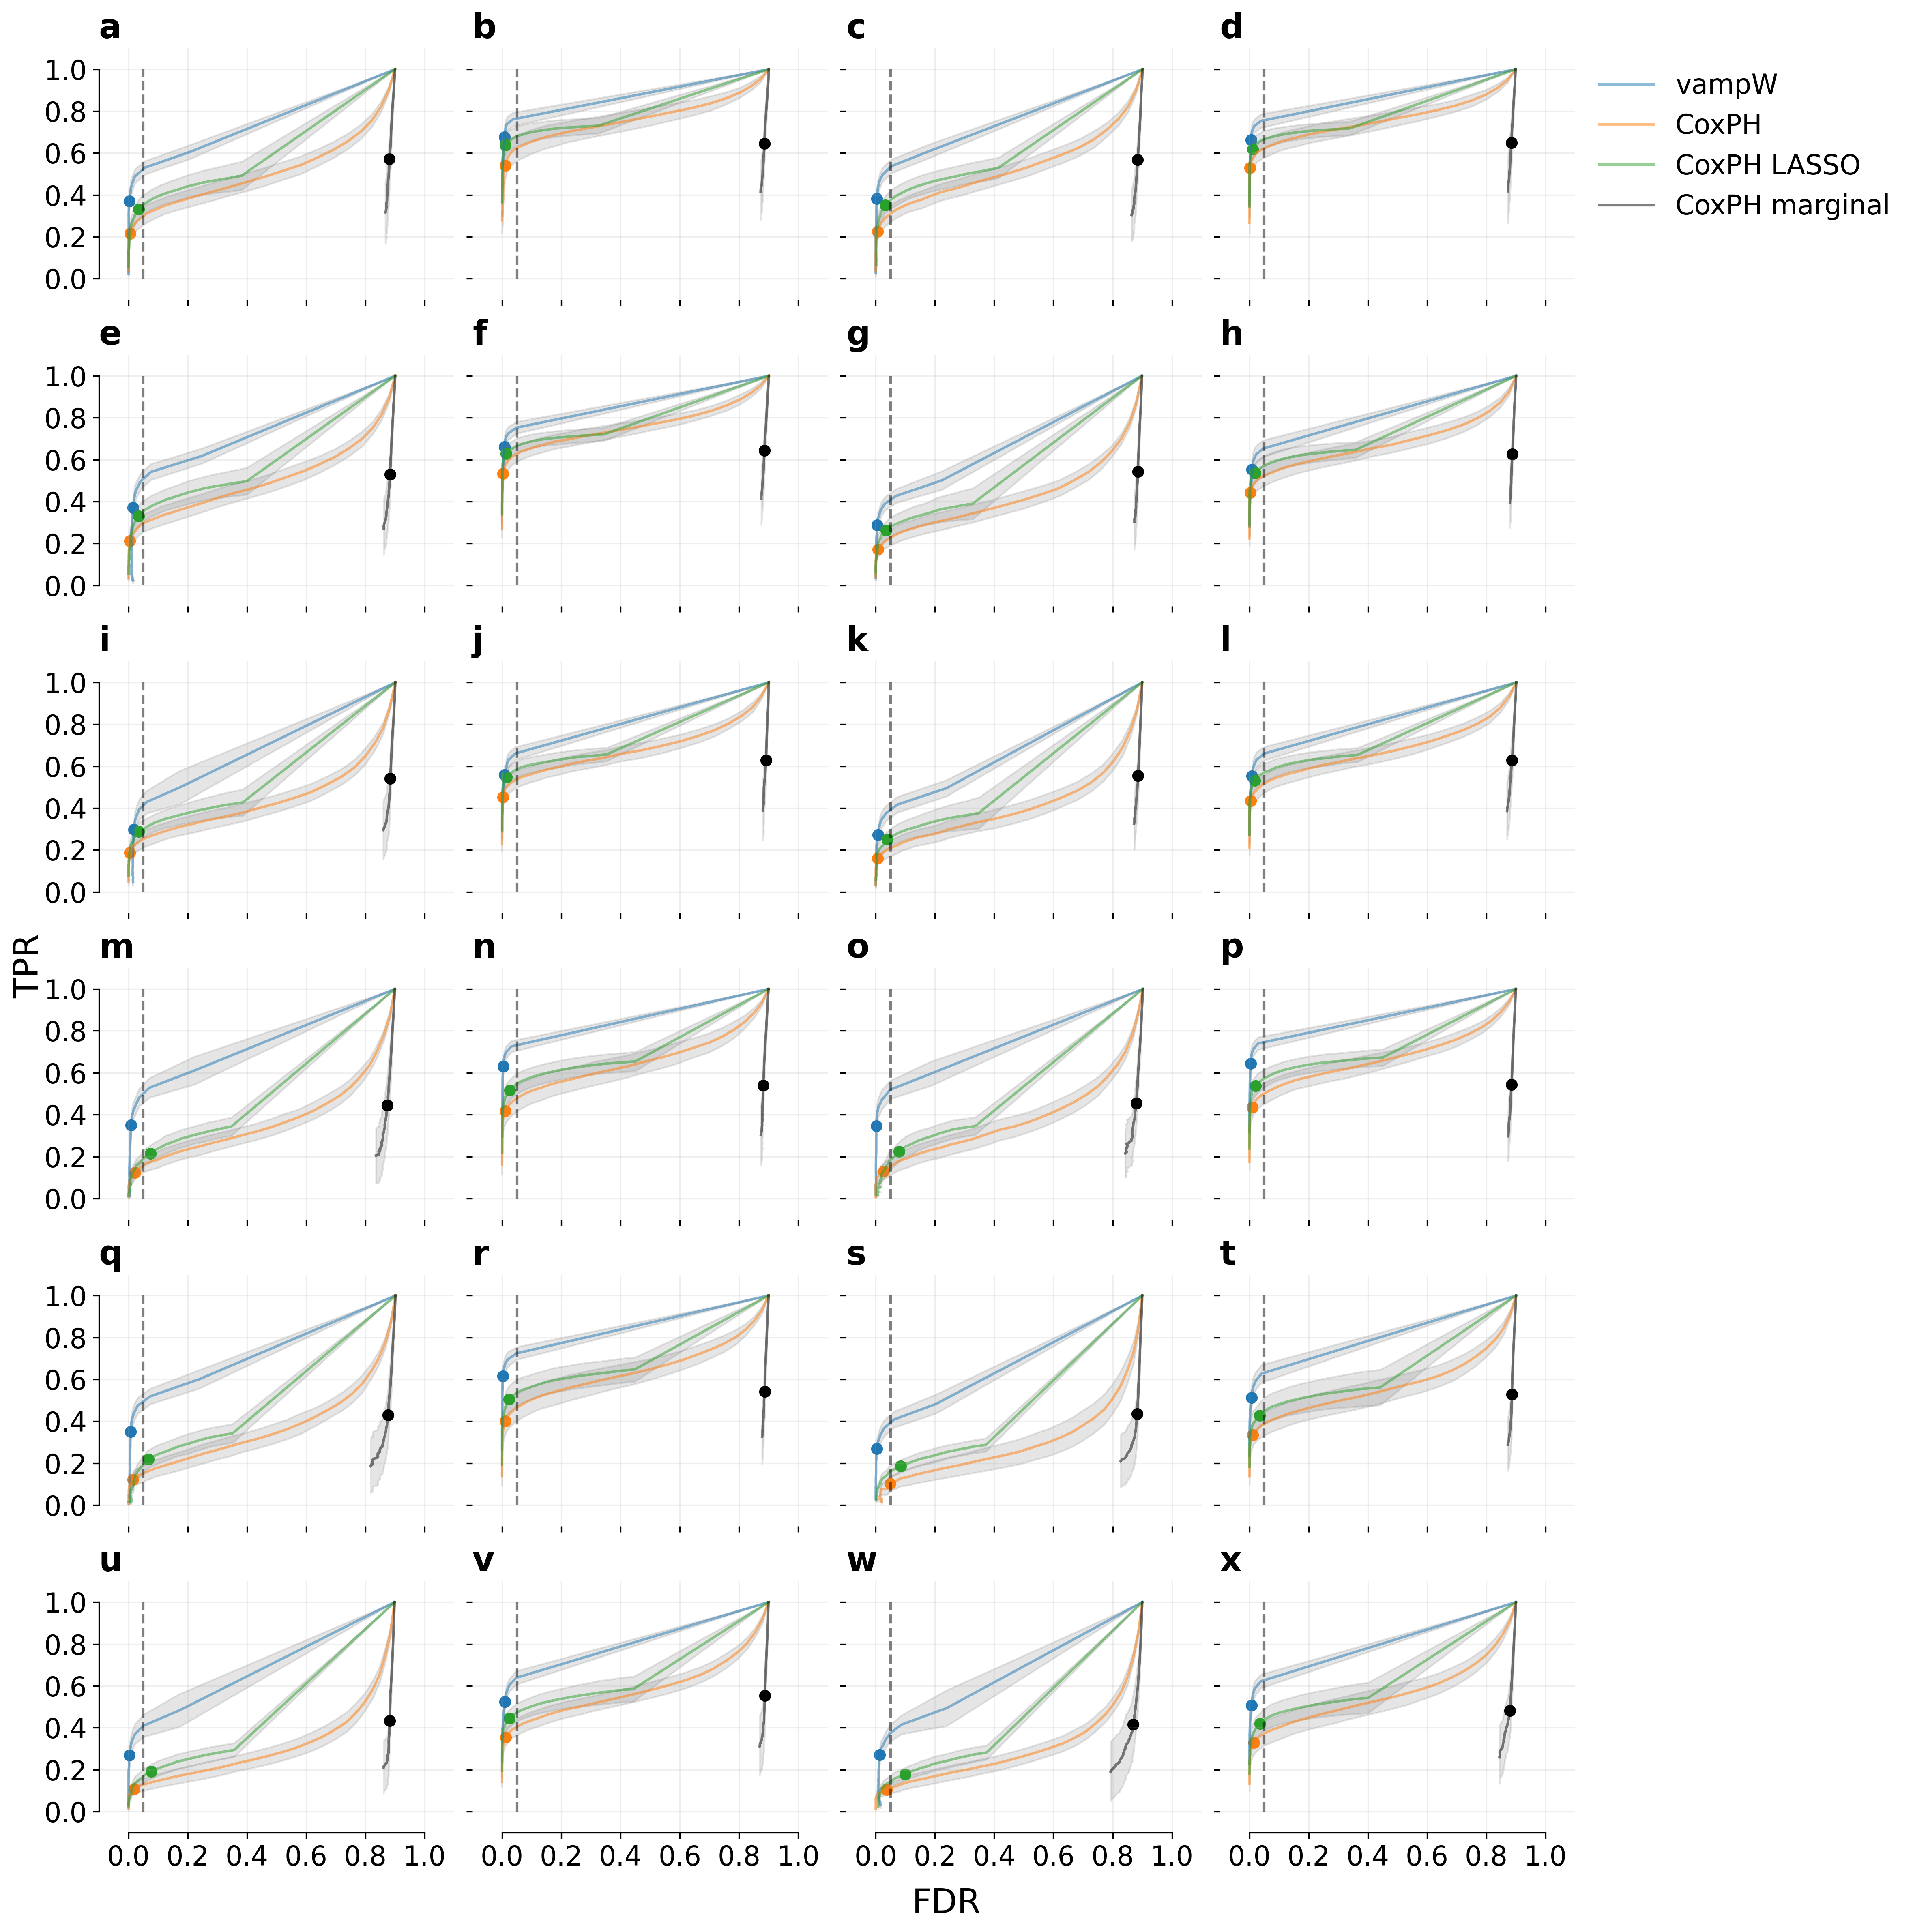
\includegraphics[width=\linewidth]{figures/sim_fdr_tpr.png}
    \end{center}
    \caption[Simulation study of variable selection performance using protein data from the UK Biobank]{\textbf{Simulation study of variable selection performance using protein data from the UK Biobank.} We simulate artificial phenotypic outcomes under 24 scenarios, corresponding to the parameterizations described in Supplementary Table \ref{tab:sim}, varying the proportion of variance explained, level of censoring, phenotype distribution, and distribution of regression coefficients. We compare the variable selection performance of vampW against several benchmarking methods (CoxPH, CoxPH LASSO and CoxPH marginal) in terms of the relationship between the false discovery rate (FDR) and true positive rate (TPR). For vampW, we use posterior inclusion probabilities (PIPs), with colored dots indicating a 0.95 threshold. For the other methods, p-value testing across multiple thresholds is employed, with colored dots indicating a Bonferroni-corrected 0.05 threshold.\label{fig:fdr_tpr}}
\end{figure}

\begin{figure}[H] % the continued legend, directly after the figure (on the next page)
    \ContinuedFloat
    \captionsetup{labelformat=continued}
    \caption[]{vampW maintains a calibrated FDR and consistently outperforms CoxPH-based models in TPR across all simulation scenarios, including those involving model misspecification. The error bars (gray shaded areas) represent the standard deviation across 50 simulation replicates.}
\end{figure}

\clearpage

\begin{figure}[H]
    \begin{center}
        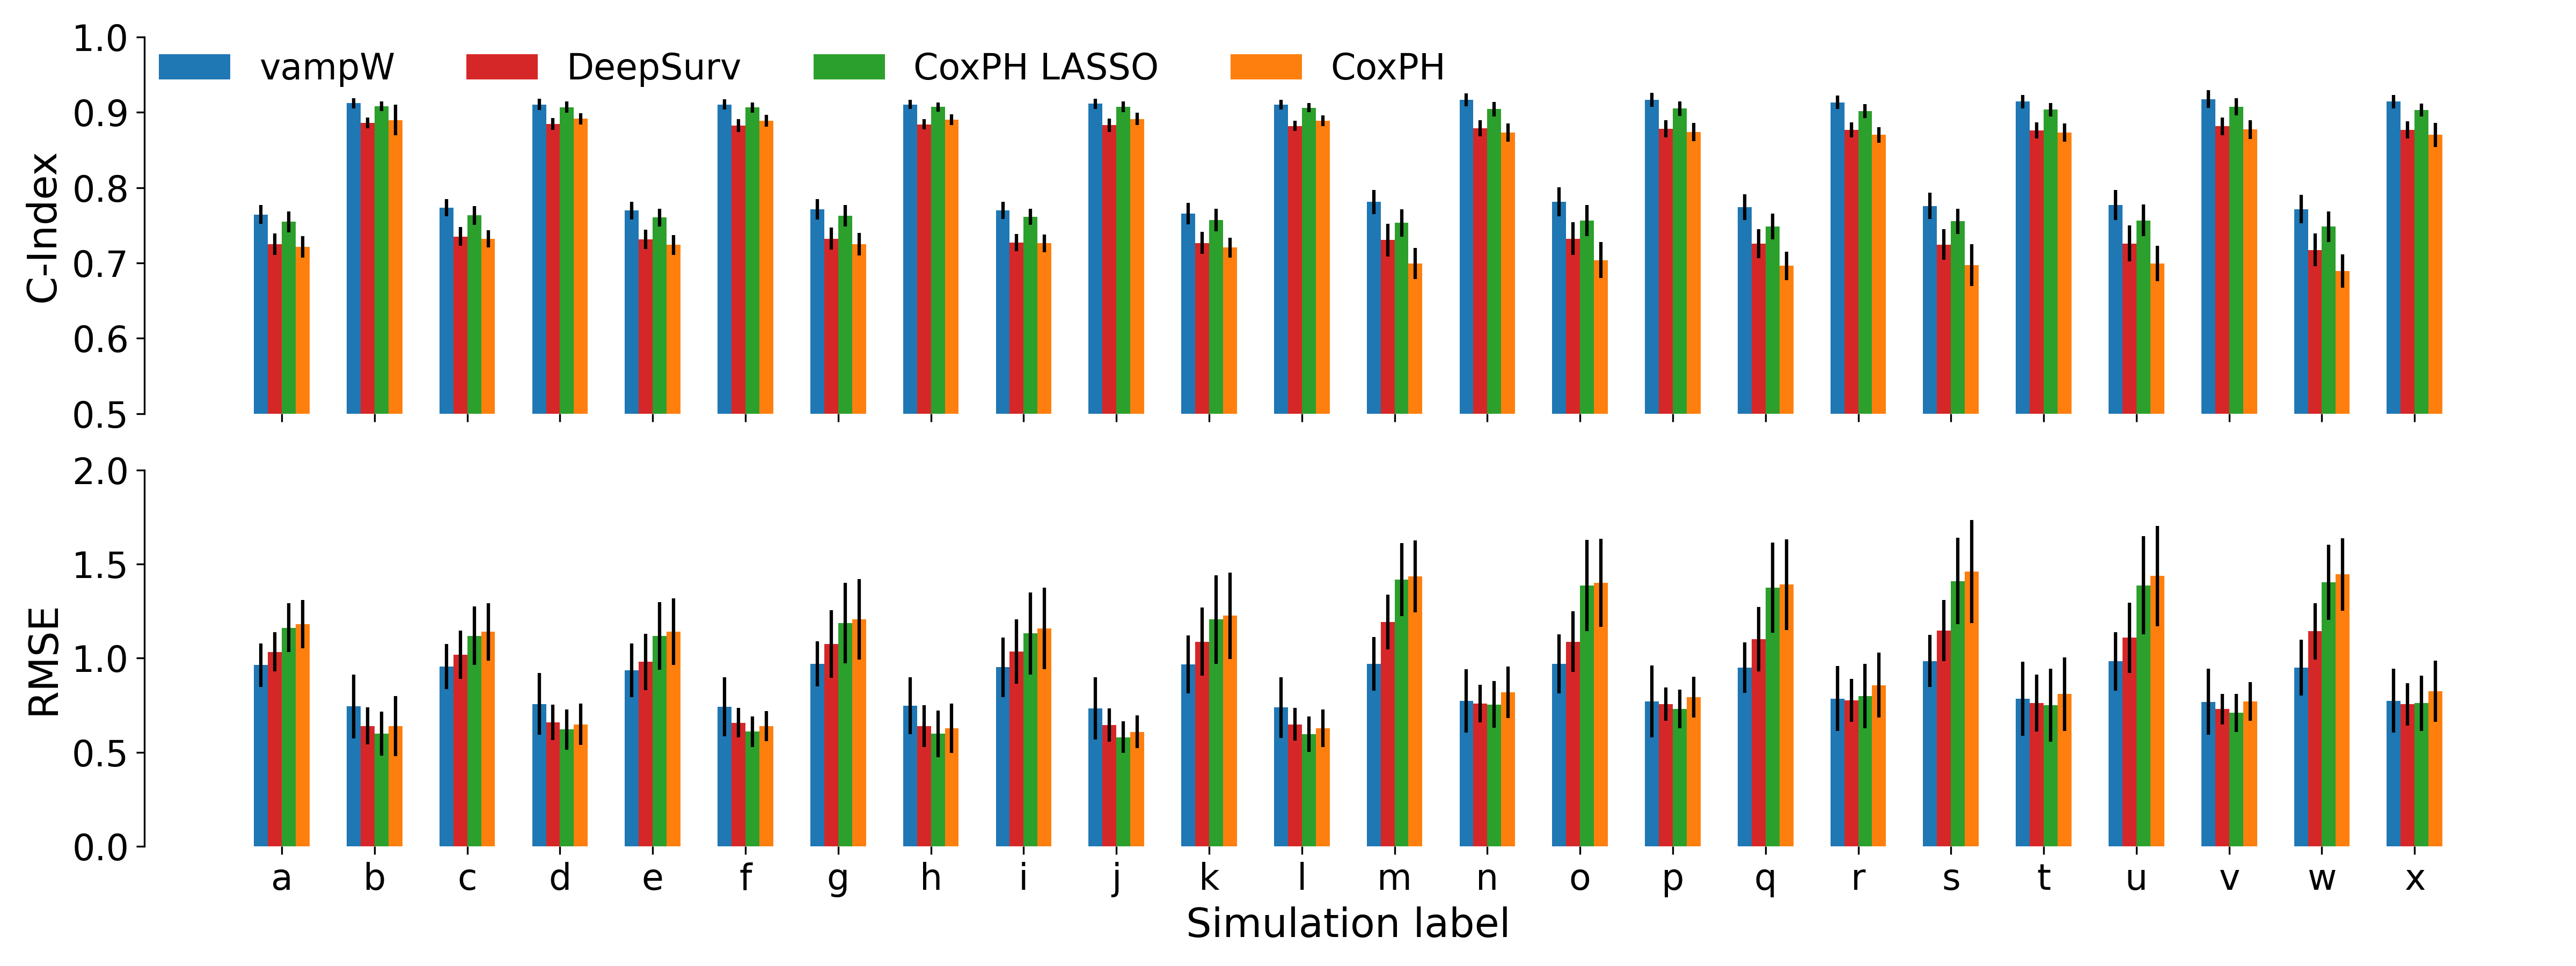
\includegraphics[width=\linewidth]{figures/sim_prediction.png}
    \end{center}
        \caption[Simulation study of out-of-sample prediction performance using protein data from the UK Biobank]{\textbf{Simulation study of out-of-sample prediction performance using protein data from the UK Biobank.} We evaluate predictive performance for time of onset across 24 simulated phenotypic outcomes corresponding to the parameterizations in Supplementary Table \ref{tab:sim}. We compare vampW with CoxPH, CoxPH LASSO, and DeepSurv in terms of concordance index (C-index) and root mean squared error (RMSE). The RMSE is evaluated in the logarithmic domain, assuming standardized outcomes with zero mean and unit variance. Across all simulated scenarios, vampW consistently demonstrates a clear improvement in the C-index when compared to both DeepSurv and the standard CoxPH model. When compared to CoxPH LASSO, the point estimate of C-index values for vampW improves, although it remains within overlapping error bars across all scenarios. In terms of RMSE, vampW strictly outperforms the standard CoxPH model in six scenarios and improves upon CoxPH LASSO in five scenarios. In all remaining comparisons, the predictive performance of the evaluated methods falls within each other's error margins. The reported error bars represent the standard deviation across 50 simulation replicates (black lines at the top of the colored bars). 
        \label{fig:sim_prediction}}
\end{figure}

\clearpage


\begin{figure}[H]
\begin{center}
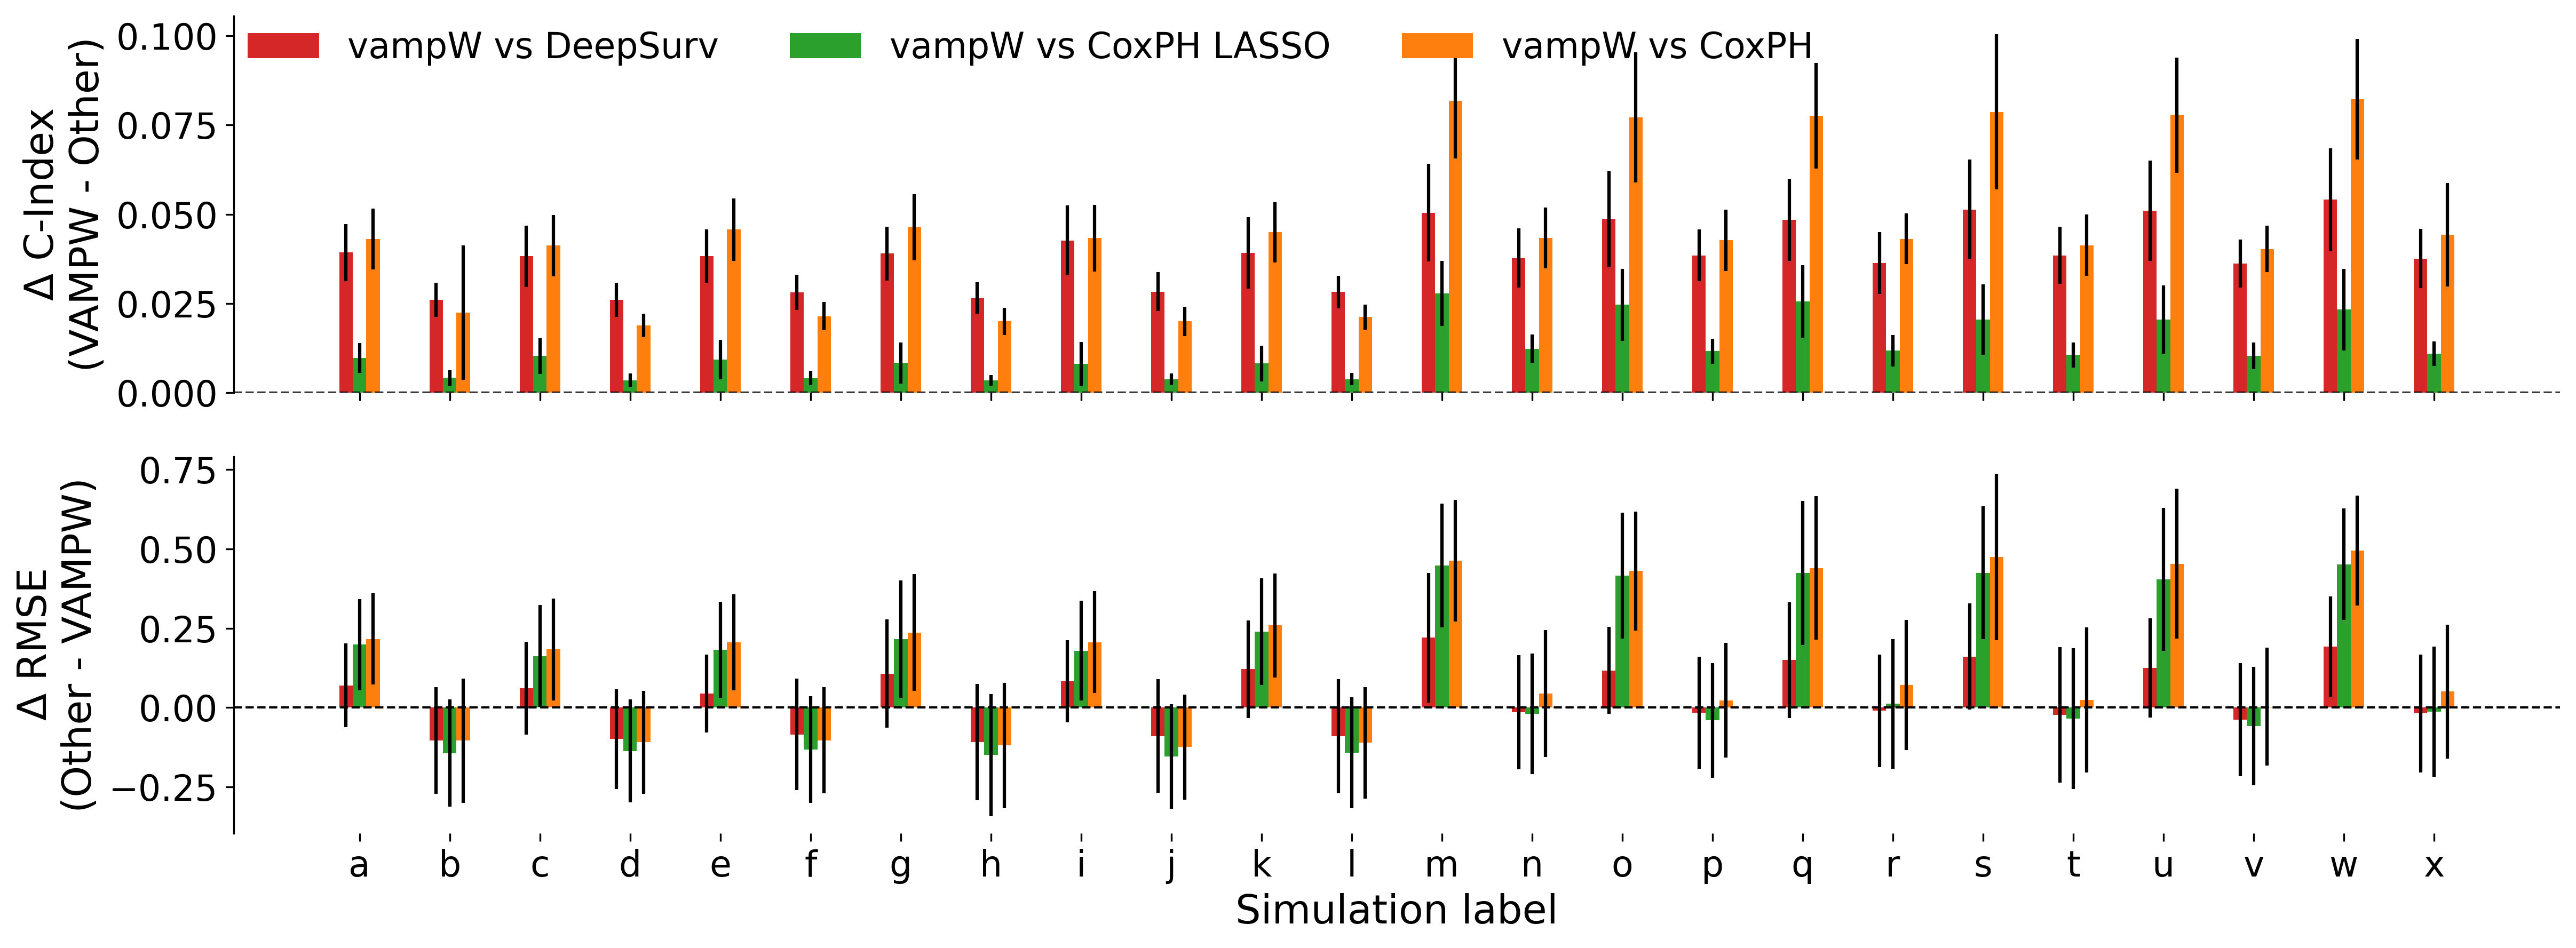
\includegraphics[width=\linewidth]{figures/sim_paired_differences.png}
\end{center}
% \caption{\textbf{Paired differences in out-of-sample prediction performance across simulated phenotypic outcomes.} We evaluate predictive performance of vampW compared to DeepSurv, CoxPH LASSO, and the standard CoxPH model across 24 simulated scenarios (corresponding to the parameterizations in Table \ref{tab:sim}). The top panel displays the paired difference in concordance index ($\Delta$ C-index), calculated as VAMPW minus the competing method. The bottom panel shows the paired difference in root mean squared error ($\Delta$ RMSE), calculated as the competing method minus VAMPW. By this formulation, consistent positive values in both panels (bars extending above the dashed zero line) would indicate superior predictive performance of vampW compared to other benchmarking methods. The RMSE is evaluated in the logarithmic domain, assuming standardized outcomes with zero mean and unit variance. The reported error bars represent the standard deviation of the paired differences across 50 simulation replicates (black lines at the top or bottom of the colored bars). In terms of C-index vampW, paired difference with error bars never crosses zero threshold indicating that vampW is outperforming other methods across all scenarios.  In terms of RMSE, vampW is always on par with the competitor methods or outperforming them.
% \label{fig:sim_paired_differences}}
% \end{figure}
\caption[Paired differences in out-of-sample prediction performance across simulated phenotypic outcomes]{\textbf{Paired differences in out-of-sample prediction performance across simulated phenotypic outcomes.} We evaluate the predictive performance of vampW compared to DeepSurv, CoxPH LASSO, and the standard CoxPH model across 24 simulated scenarios (corresponding to the parameterizations in Supplementary Table \ref{tab:sim}). The top panel displays the paired difference in concordance index ($\Delta$ C-index), calculated as vampW minus the competing method. The bottom panel shows the paired difference in root mean squared error ($\Delta$ RMSE), calculated as the competing method minus vampW. By this formulation, positive values in both panels (bars extending above the dashed zero line) indicate superior predictive performance by vampW. The RMSE is evaluated in the logarithmic domain, assuming standardized outcomes with zero mean and unit variance. The reported error bars represent the standard deviation of the paired differences across 50 simulation replicates (black lines at the top or bottom of the colored bars). For the C-index, the paired differences, inclusive of error bars, never cross the zero threshold, indicating that vampW consistently outperforms the other methods across all scenarios. In terms of RMSE, vampW achieves performance that is either on par with or superior to the competing methods.
}
\label{fig:sim_paired_differences}
\end{figure}

\clearpage

\begin{figure}[H]
    \begin{center}
        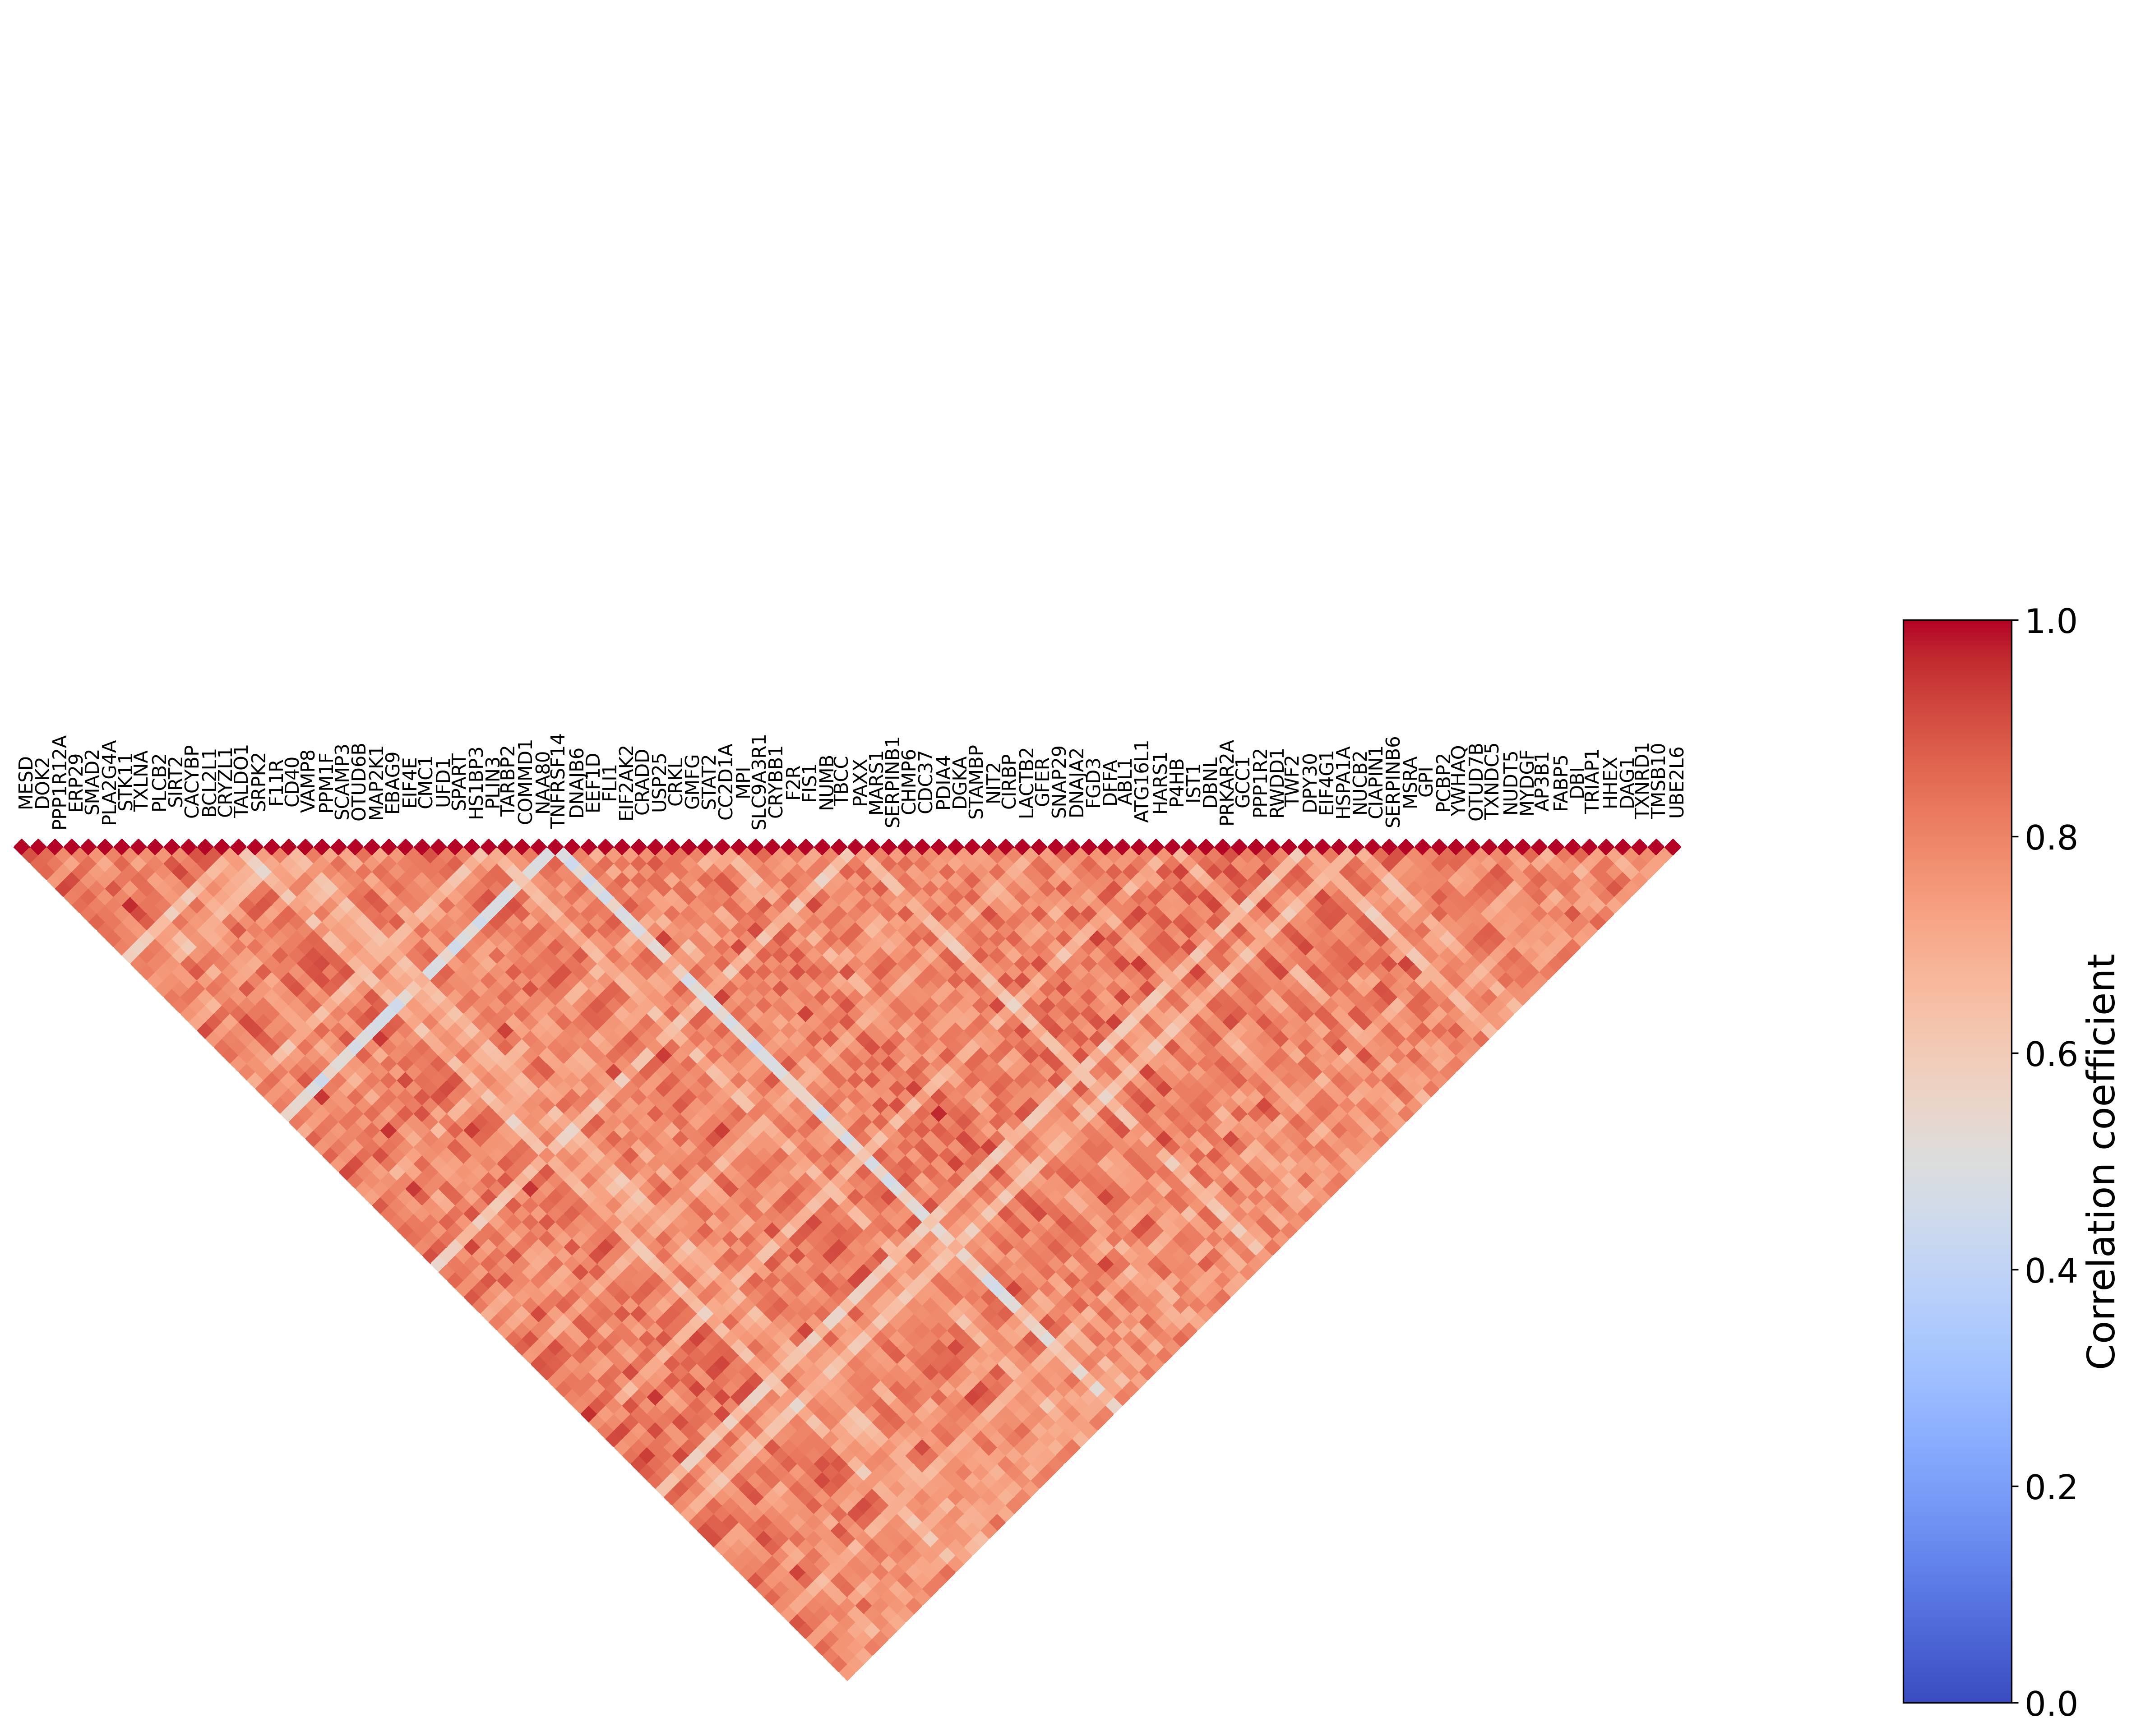
\includegraphics[width=\linewidth]{figures/corr_mat.png}
    \end{center}
    \caption[Correlation structure of the protein measures in the UK Biobank]{\textbf{Correlation structure of the protein measures in the UK Biobank.} We calculate Pearson product-moment correlation coefficients for all proteins, not-adjusted for covariates, and select the top 100 most correlated ones. We plot the correlation structure along with corresponding protein-coding genes.\label{fig:correlation}}
\end{figure}

\clearpage

\begin{figure}[H]
    \begin{center}
        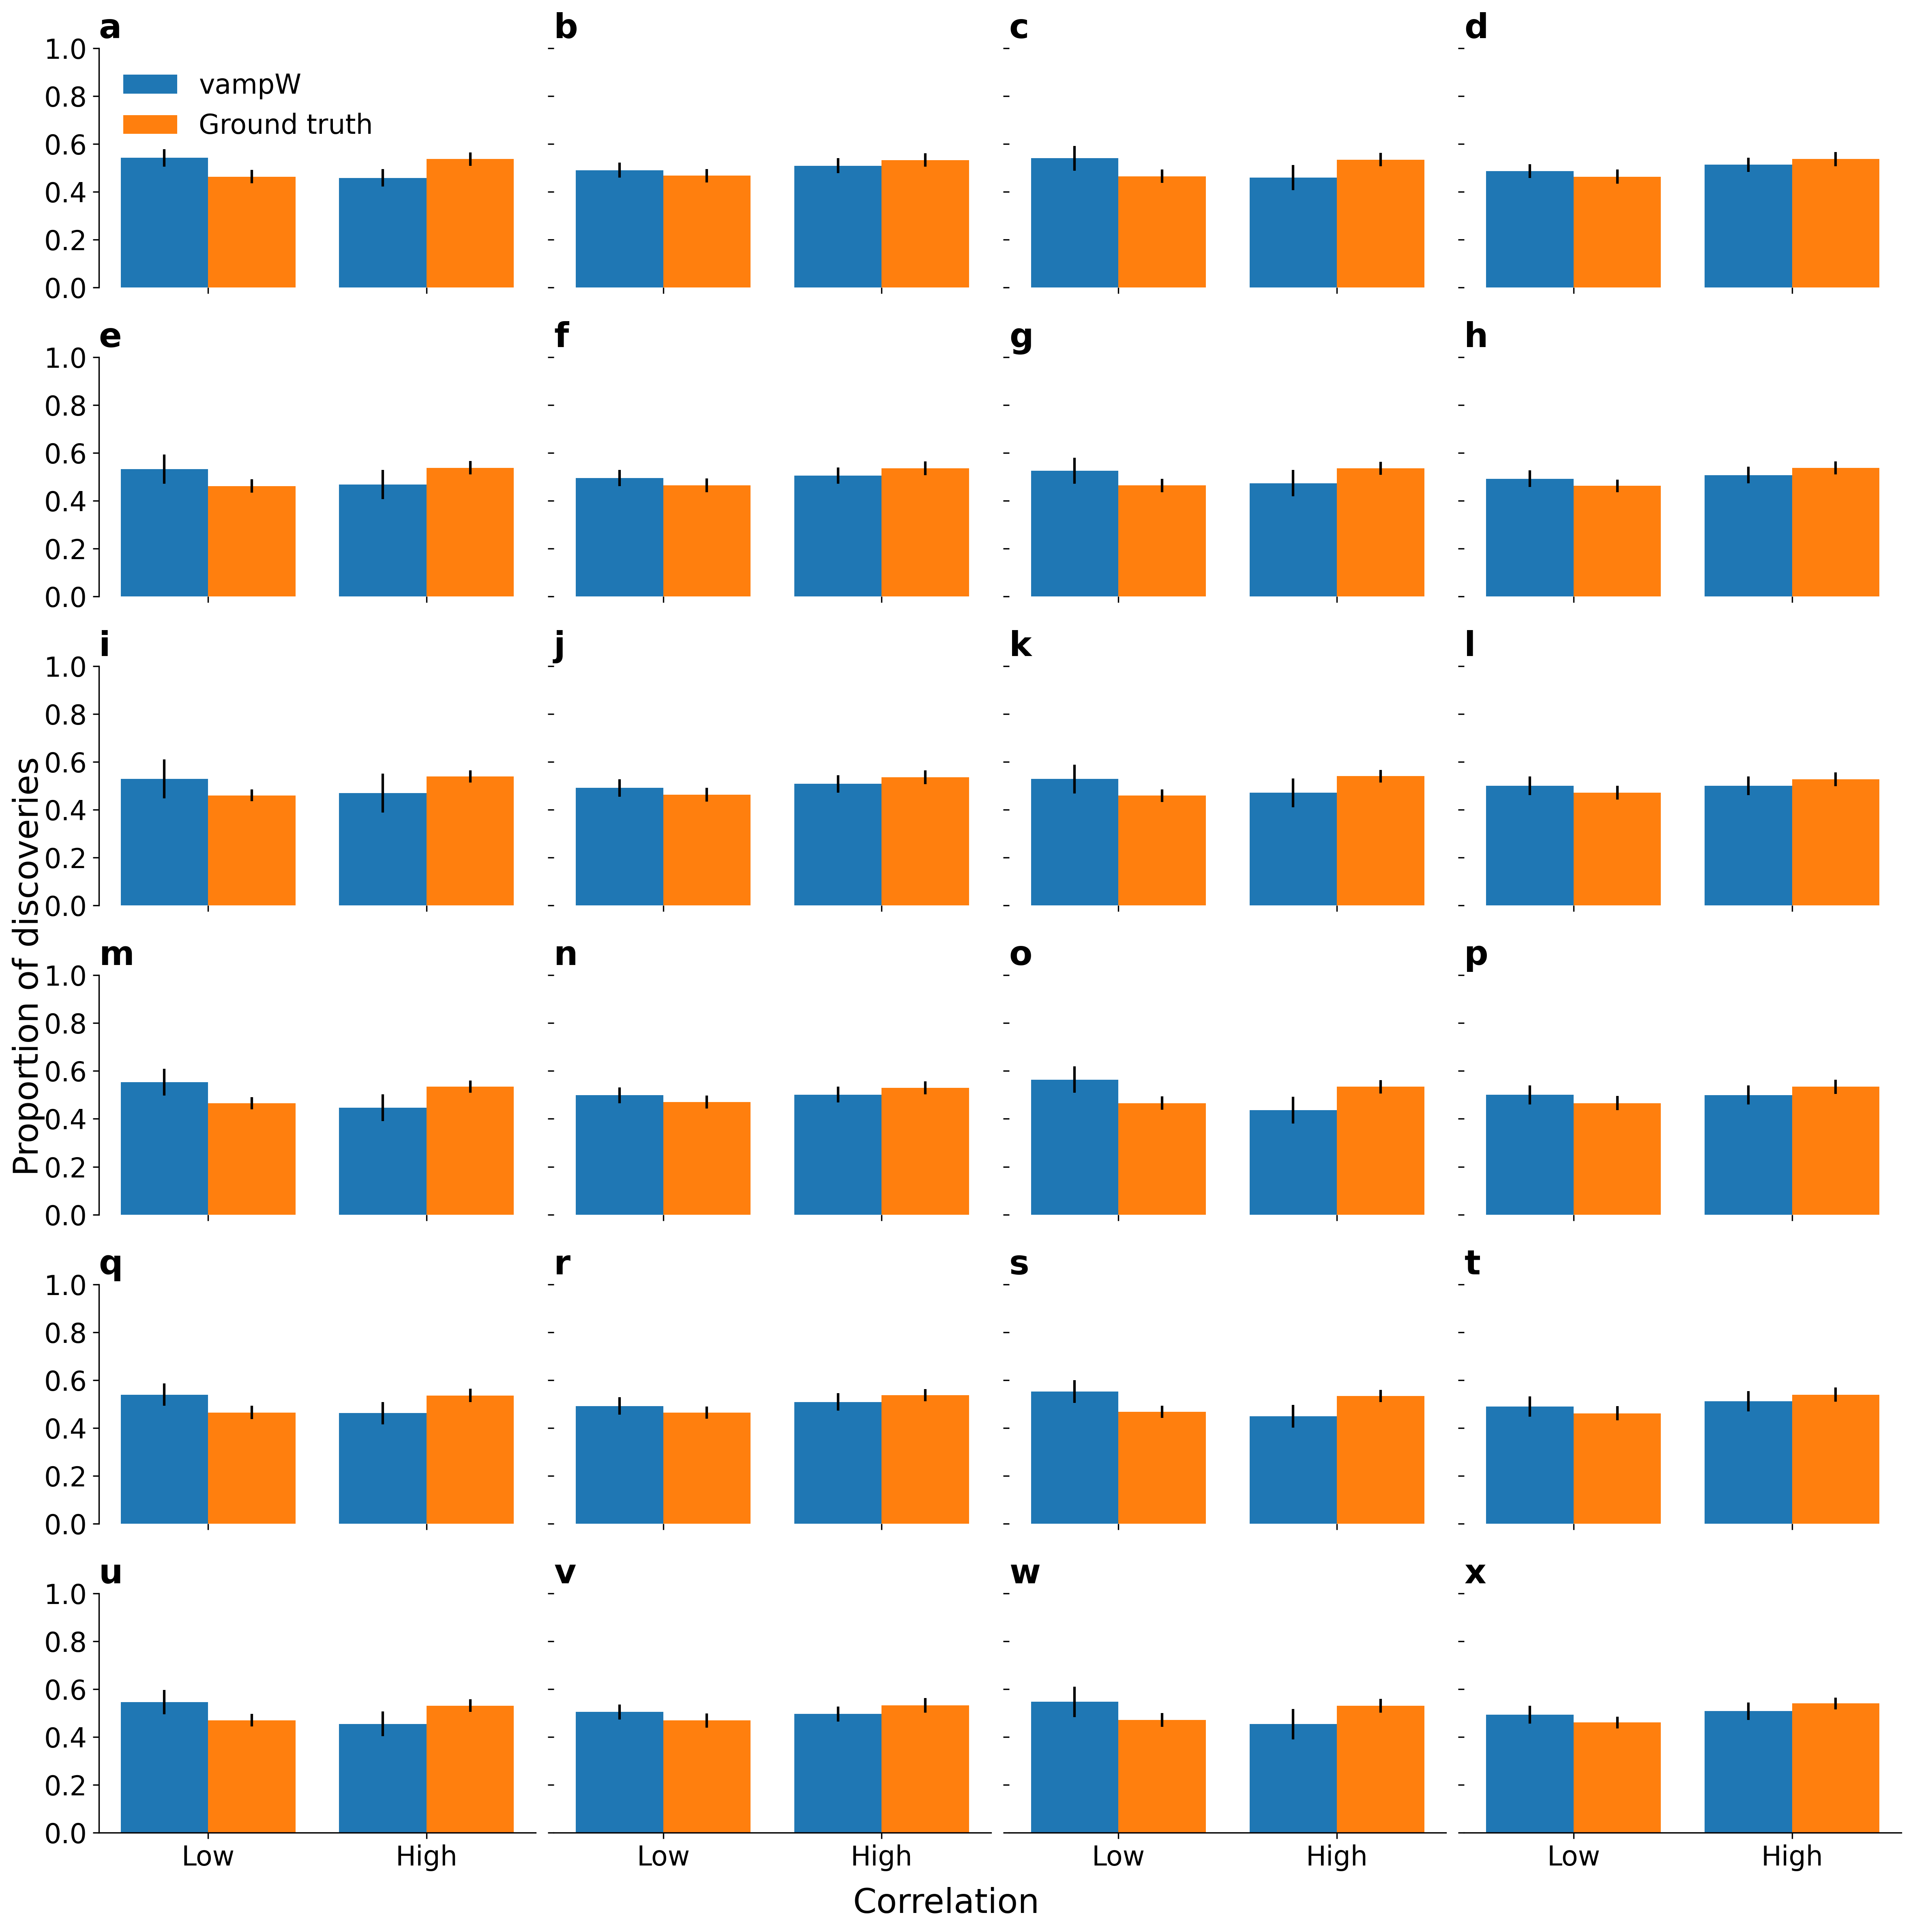
\includegraphics[width=\linewidth]{figures/sim_annot.png}
    \end{center}
    \caption[Protein annotation based on correlation structure]{\textbf{Protein annotation based on correlation structure}. For 24 simulation scenarios, described in Supplementary Table \ref{tab:sim}, we visualize the relative proportion of highly and low-correlated true positive discoveries with respect to all true positive discoveries (blue), and compare this to the proportion of highly and low-correlated causal proteins with respect to all causal proteins (orange). If the correlation of a particular protein with any other protein is greater than 0.5 (absolute value of Pearson correlation coefficient), it is categorized as a highly correlated protein. The remaining proteins are categorized as low-correlated. The black bars show 1 standard error over 50 simulation replicas. The results suggest that vampW detects causal signals even for proteins with correlations above the 0.5 threshold.
\label{fig:annot}}
\end{figure}

\clearpage

\begin{figure}[H]
    \begin{center}
        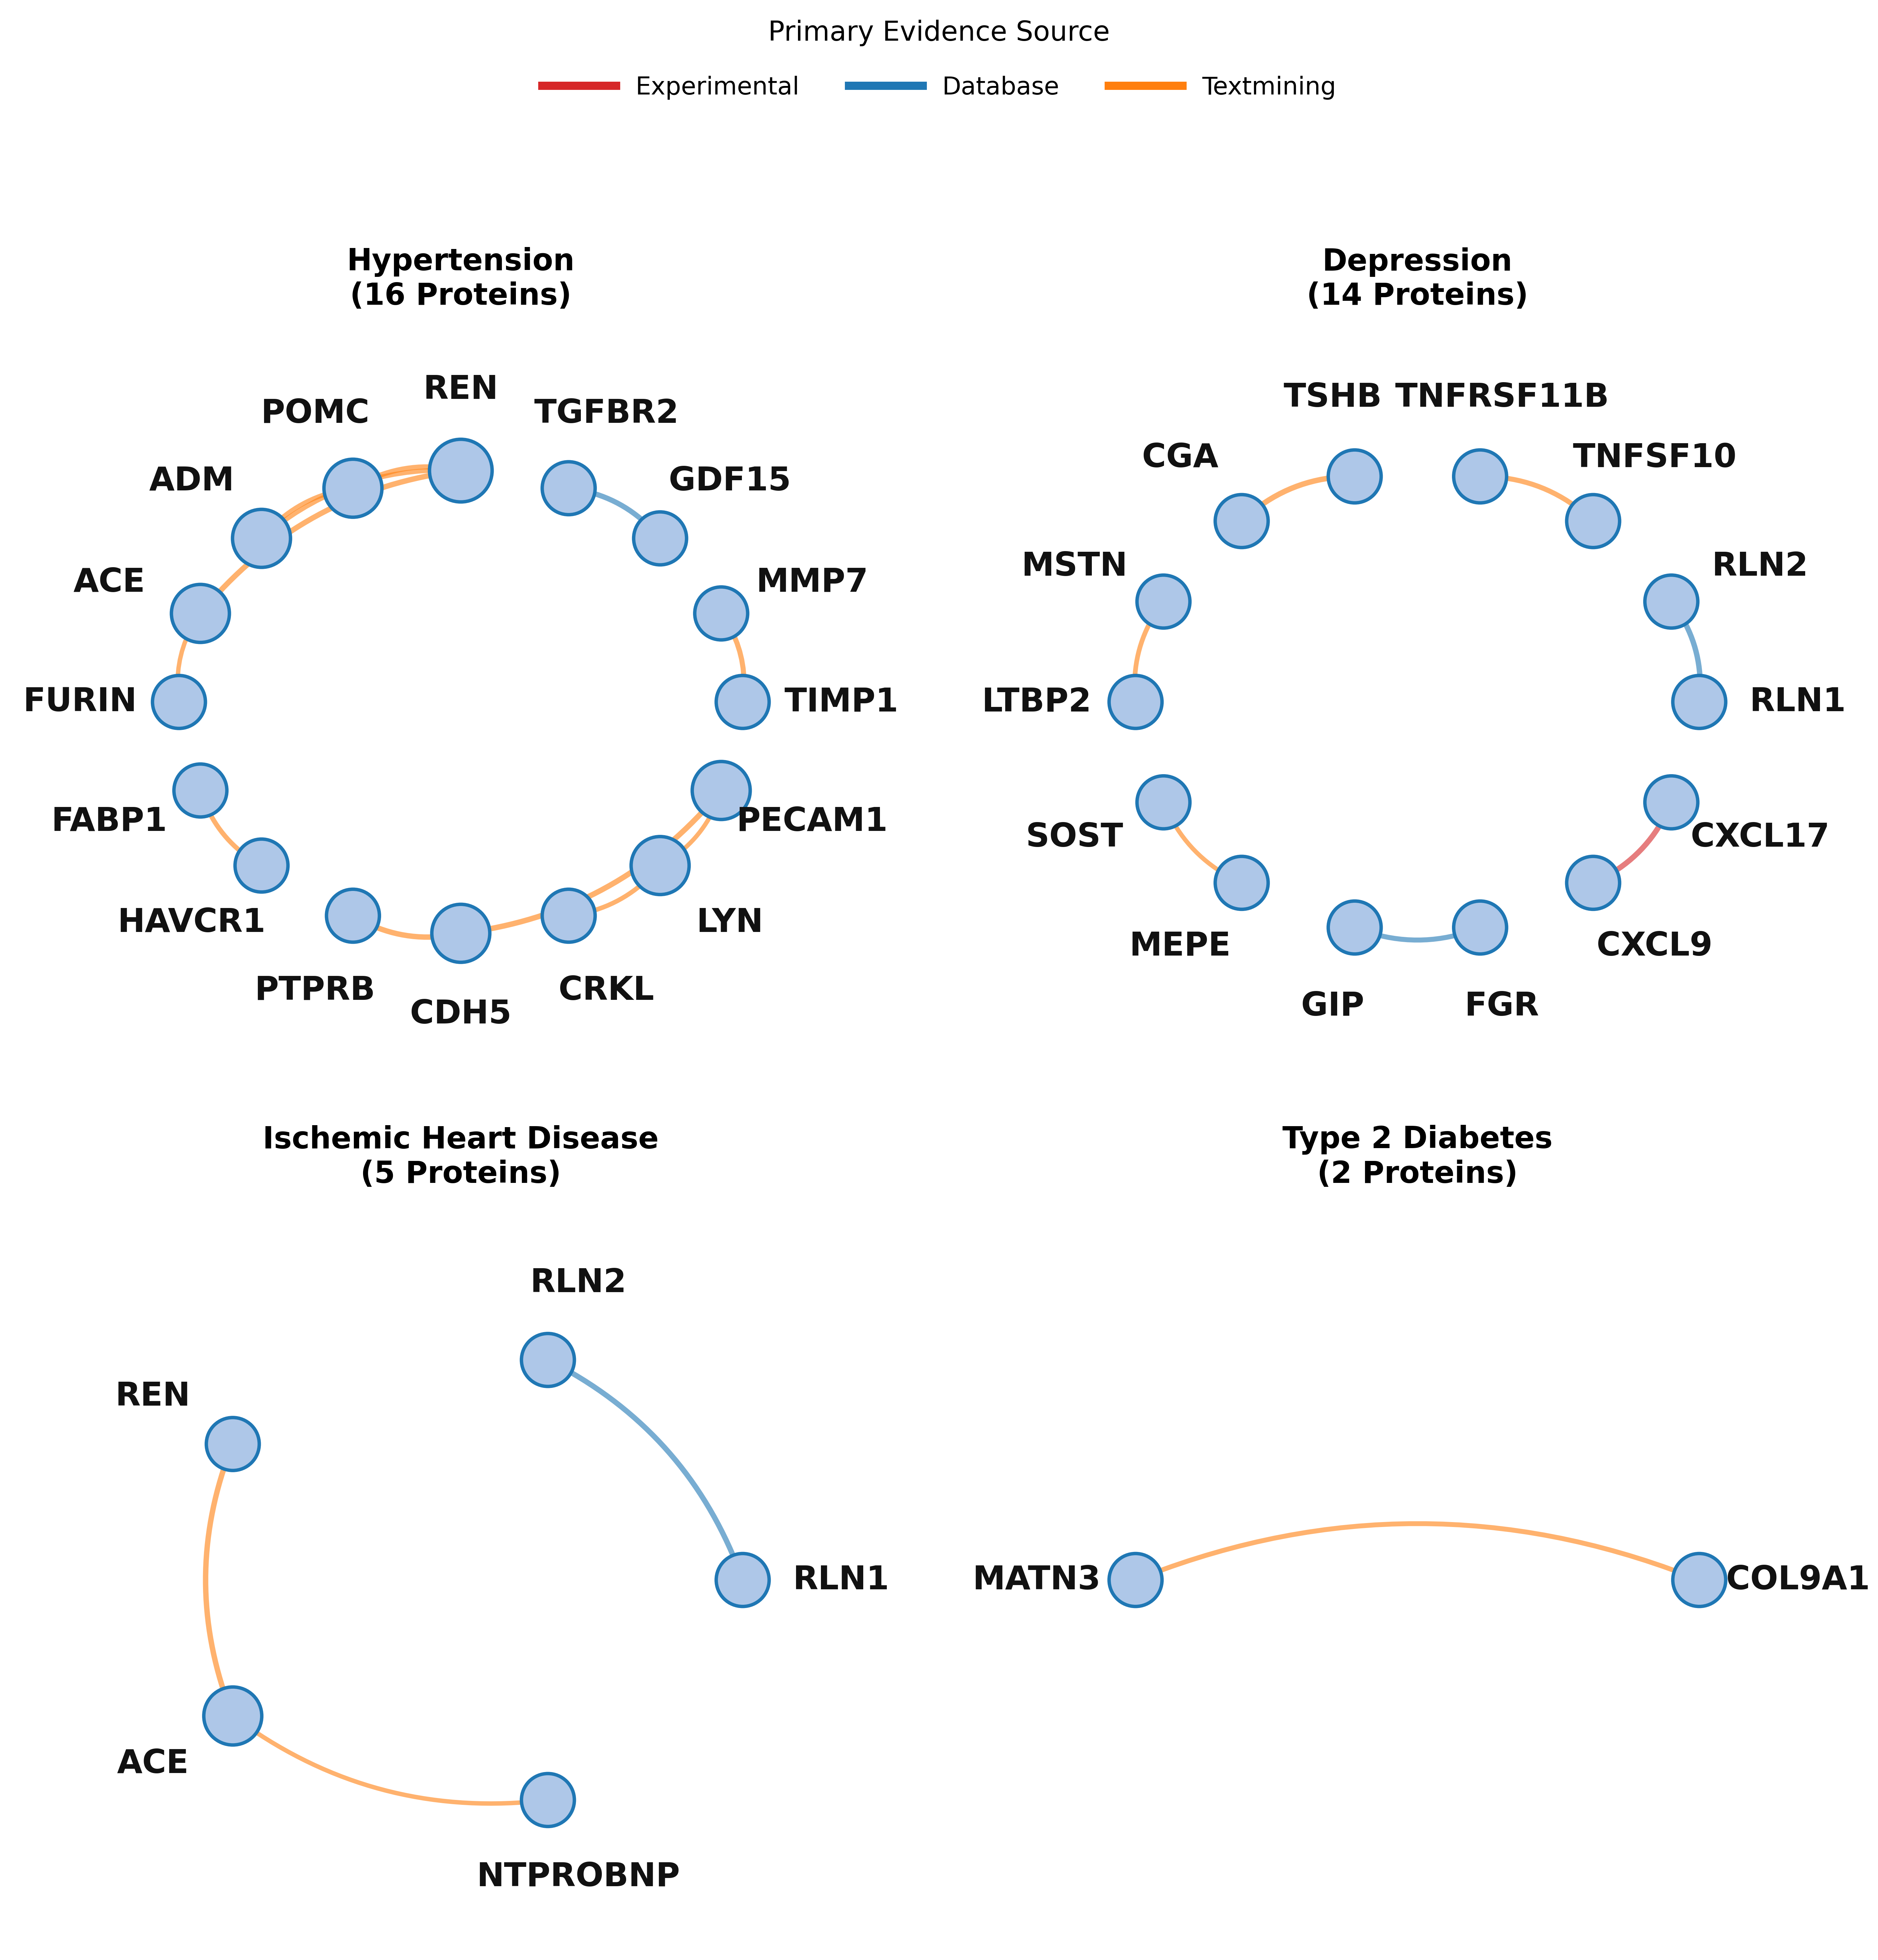
\includegraphics[width=\linewidth]{figures/summary_panel_plot.png}
    \end{center}
    \caption[Protein-protein interaction networks for trait-associated proteins]{\textbf{Protein-protein interaction networks for trait-associated proteins.} Network visualizations of significant proteins associated with Hypertension, Depression, Ischemic Heart Disease, and Type 2 Diabetes. Nodes represent individual proteins identified in the analysis. Edges denote known interactions retrieved from the STRING database (version 12.0), filtered for high-confidence connections (combined score $\ge 800$). Edge colors indicate the primary source of evidence supporting the interaction: experimental validation (red), curated databases (blue), or automated text mining (orange). Node sizes are proportionally scaled by their degree (number of connections) within the local trait network. Proteins without high-confidence interactions in the selected sub-network are excluded from the visualization.}\label{fig:interaction_networks}

\end{figure}

\clearpage

\begin{figure}[H]
    \begin{center}
        \includegraphics[width=\linewidth]{figures/cov_lin_exp.png}
    \end{center}
    \caption[Adjusting for non-linear effects of age on protein levels]{\textbf{Adjusting for non-linear effects of age on protein levels}.  In addition to the standard linear adjustment (blue) for the age covariate, we evaluate the vampW model using protein data adjusted for exponential age effects (orange). In column (a), we show significant protein-coding genes at their corresponding DNA positions that pass a PIP threshold of 0.95 for four representative outcomes, namely Alzheimer's disease, ischemic heart disease, colorectal cancer, and death. In column (b), we show the relationship between PIPs passing a threshold of 0.9 across the two models, where PIP$_{lin}$ and PIP$_{exp}$ denote the standard linear and exponential age adjustments, respectively. Notably, the gene \emph{CGA}, previously reported as age-associated in recent work, disappears from the discoveries when considering non-linear effects of age on protein levels.
\label{fig:cov_age}}
\end{figure}

\clearpage

\begin{figure}[H]
    \begin{center}
        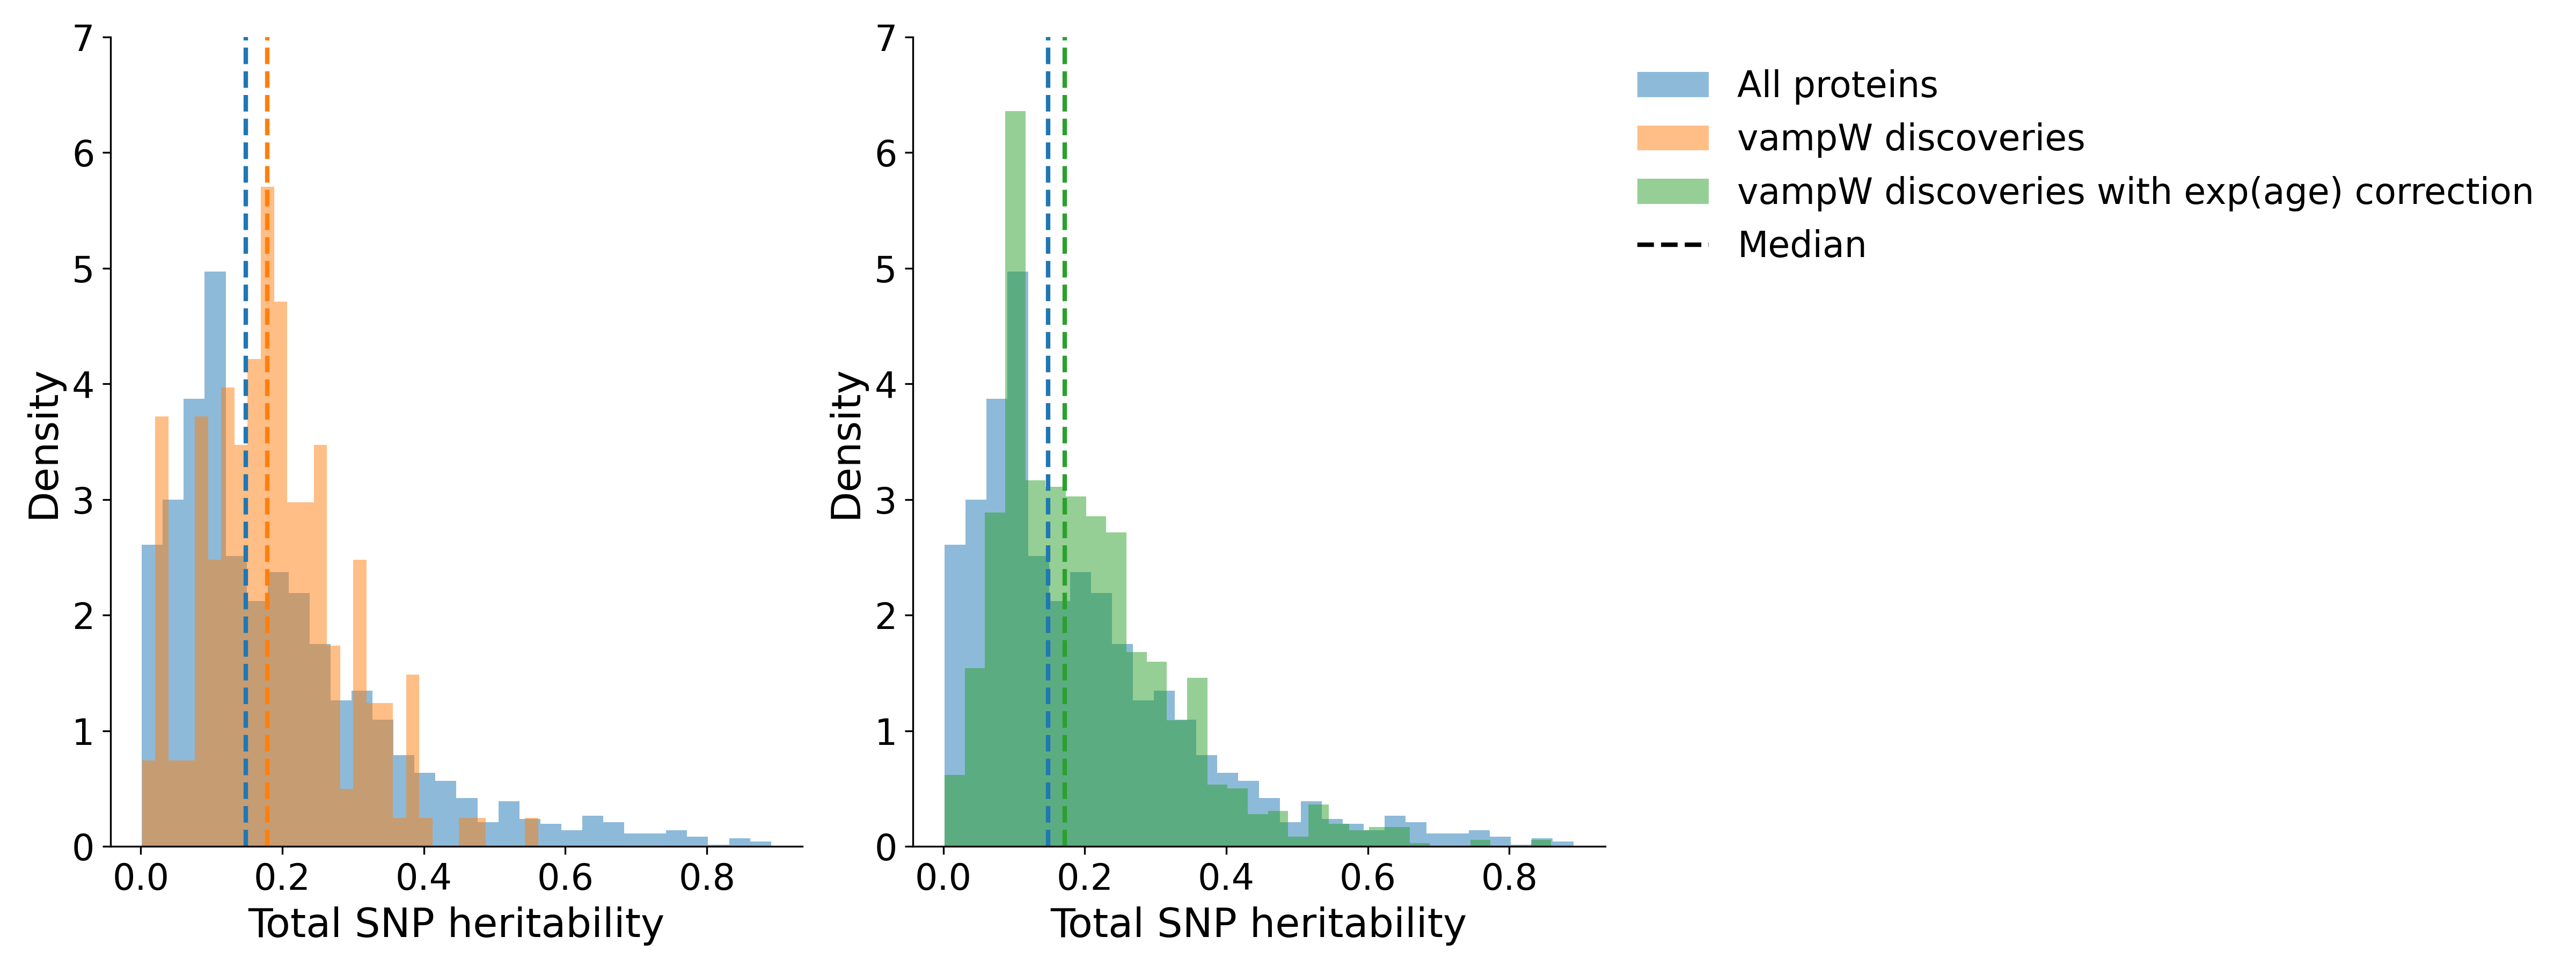
\includegraphics[width=\linewidth]{figures/protein_h2.png}
    \end{center}
    \caption[Distribution of total SNP-based heritability of proteins with pQTLs]{\changed{\textbf{Distribution of total SNP-based heritability of proteins with pQTLs.} We plot the distributions of total SNP heritability for 2,430 proteins reported in the study \cite{sun_plasma_2023}, including all proteins with pQTLs (blue) and the corresponding subset overlapping with vampW discoveries, with (green) and without (orange) exponential age correction. The vampW discoveries exhibit average heritability of 19.9\% and 18.7\% for models with and without exponential age correction, respectively, compared to a mean heritability of 19.5\% across all proteins with pQTLs.}}\label{fig:protein_h2}
\end{figure}

\clearpage

\begin{figure}[H]
    \begin{center}
        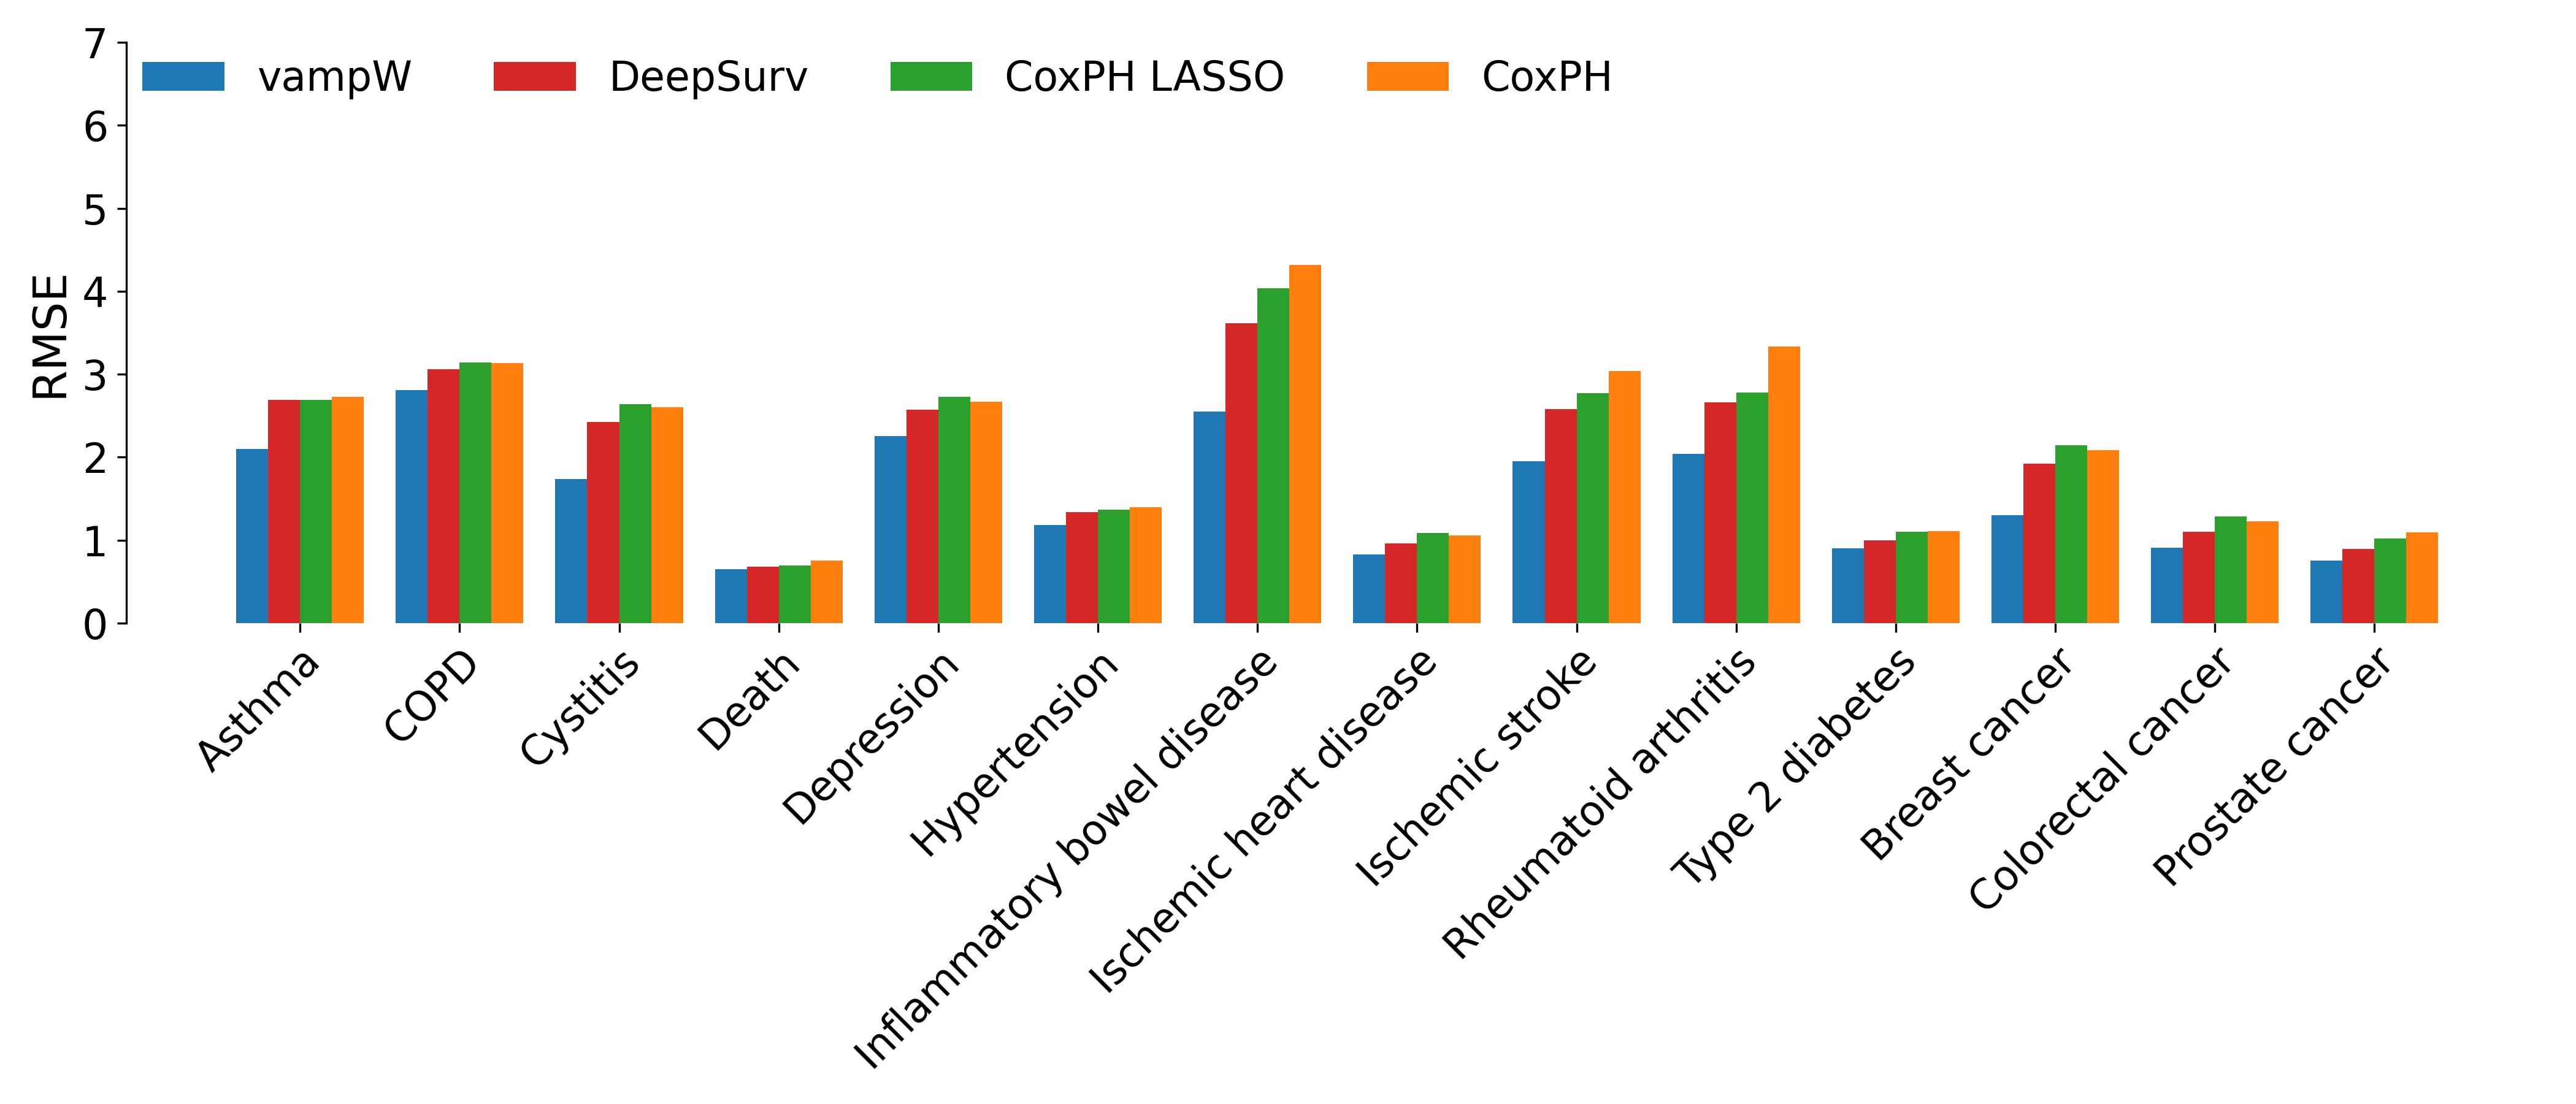
\includegraphics[width=\linewidth]{figures/real_rmse_time.png}
    \end{center}
    \caption[Out-of-sample performance comparison in terms of RMSE on the log-normalized times for CoxPH, LASSO-penalized CoxPH, DeepSurv, and vampW]{\textbf{Out-of-sample performance comparison in terms of RMSE on the log-normalized times for CoxPH, LASSO-penalized CoxPH, DeepSurv, and vampW.}
    We evaluate time-to-diagnosis predictions for 14 health-related outcomes in the UK Biobank (traits with $\ge 100$ cases present in the test set) using protein measurements adjusted for age and sex. % using linear regression approach. 
    The accuracy of the model is assessed using the root mean squared error (RMSE). The training is performed on data that is first log-transformed and standardized to zero mean and unit variance, and then scaled back using an exponential transformation. The RMSE calculation presented in this figure is performed on the logarithmic scale in which the data is standardized, and it includes only uncensored individuals across traits.}
\label{fig:real_rmse_time}
\end{figure}

\clearpage 

\begin{figure}[H]
    \begin{center}
        \includegraphics[width=1.0\linewidth]{figures/weibull_fits_dedup.png}
    \end{center}
    \caption[Analysis of age-at-onset distributions for UK Biobank traits]{\textbf{Analysis of age-at-onset distributions for UK Biobank traits}. The histograms display the empirical distribution of age-at-onset for cases across various phenotypes in the training set. The blue bars represent the density of observed onset ages, while the solid red line indicates the fitted Weibull probability density function (PDF). Outliers were excluded from the fitting process using the Interquartile Range (IQR) method. The title of each subplot provides goodness-of-fit metrics, including the Kolmogorov-Smirnov statistic (KS), Wasserstein distance (W), and Total Variation distance (TV). \label{fig:distance} } %Additionally, the percentage of "prospective drops" is reported, indicating the proportion of cases where the age of onset occurred after the baseline assessment.}
\end{figure}

\clearpage

\begin{figure}[H]
    \begin{center}
        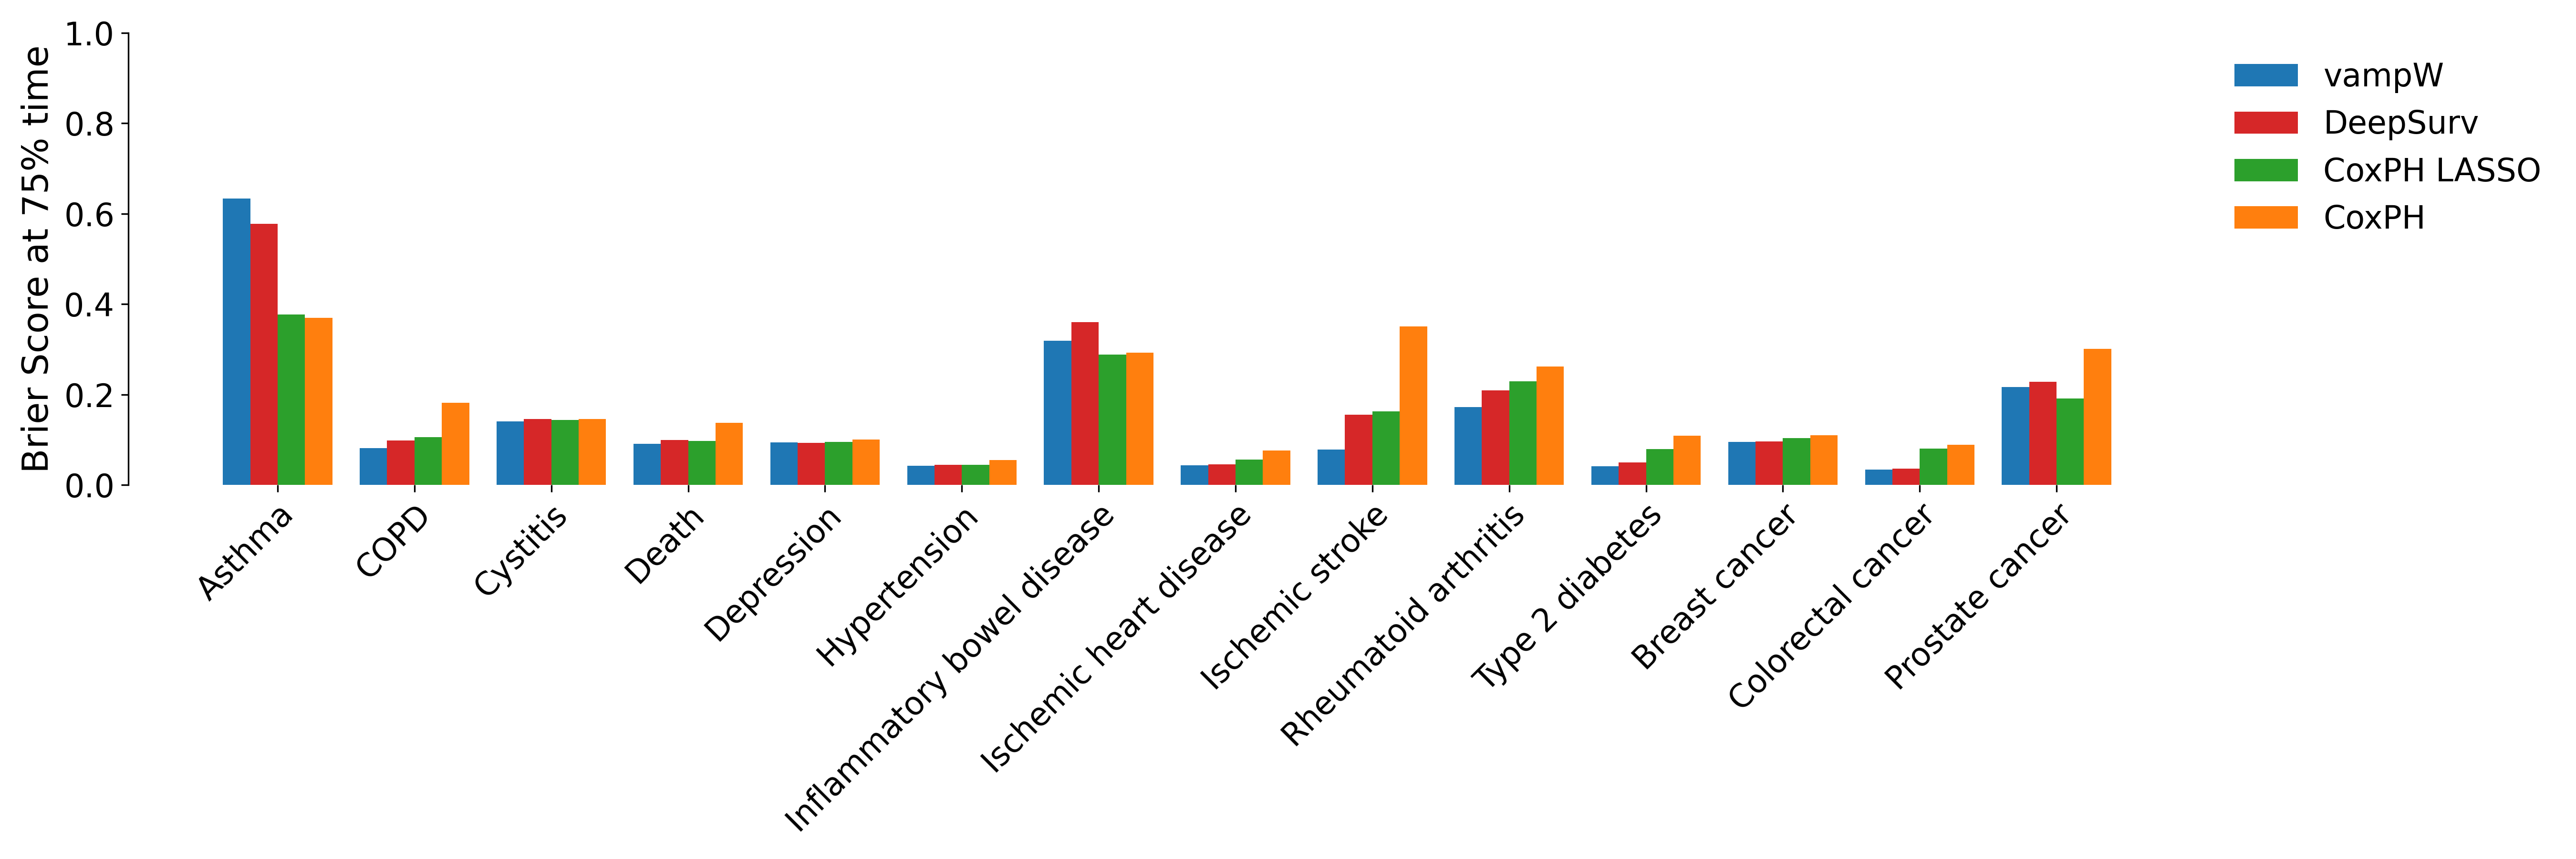
\includegraphics[width=\linewidth]{figures/bs_t75.png}
    \end{center}
    \caption[Brier Score comparison across methods evaluated at the 75\% time point]{\textbf{Brier Score comparison across methods evaluated at the 75\% time point.} We calculate the Brier Score (BS), a standard metric for evaluating the out-of-sample performance of time-to-event predictions. We report the BS value at the time corresponding to 75\% of the time span within the observed time period. Among 14 UK Biobank outcomes with sufficient sample size for out-of-sample evaluation, vampW outperforms the other benchmarking methods in 10 cases.}\label{fig:bs_t75}
\end{figure}

\clearpage

\begin{figure}[H]
    \begin{center}
        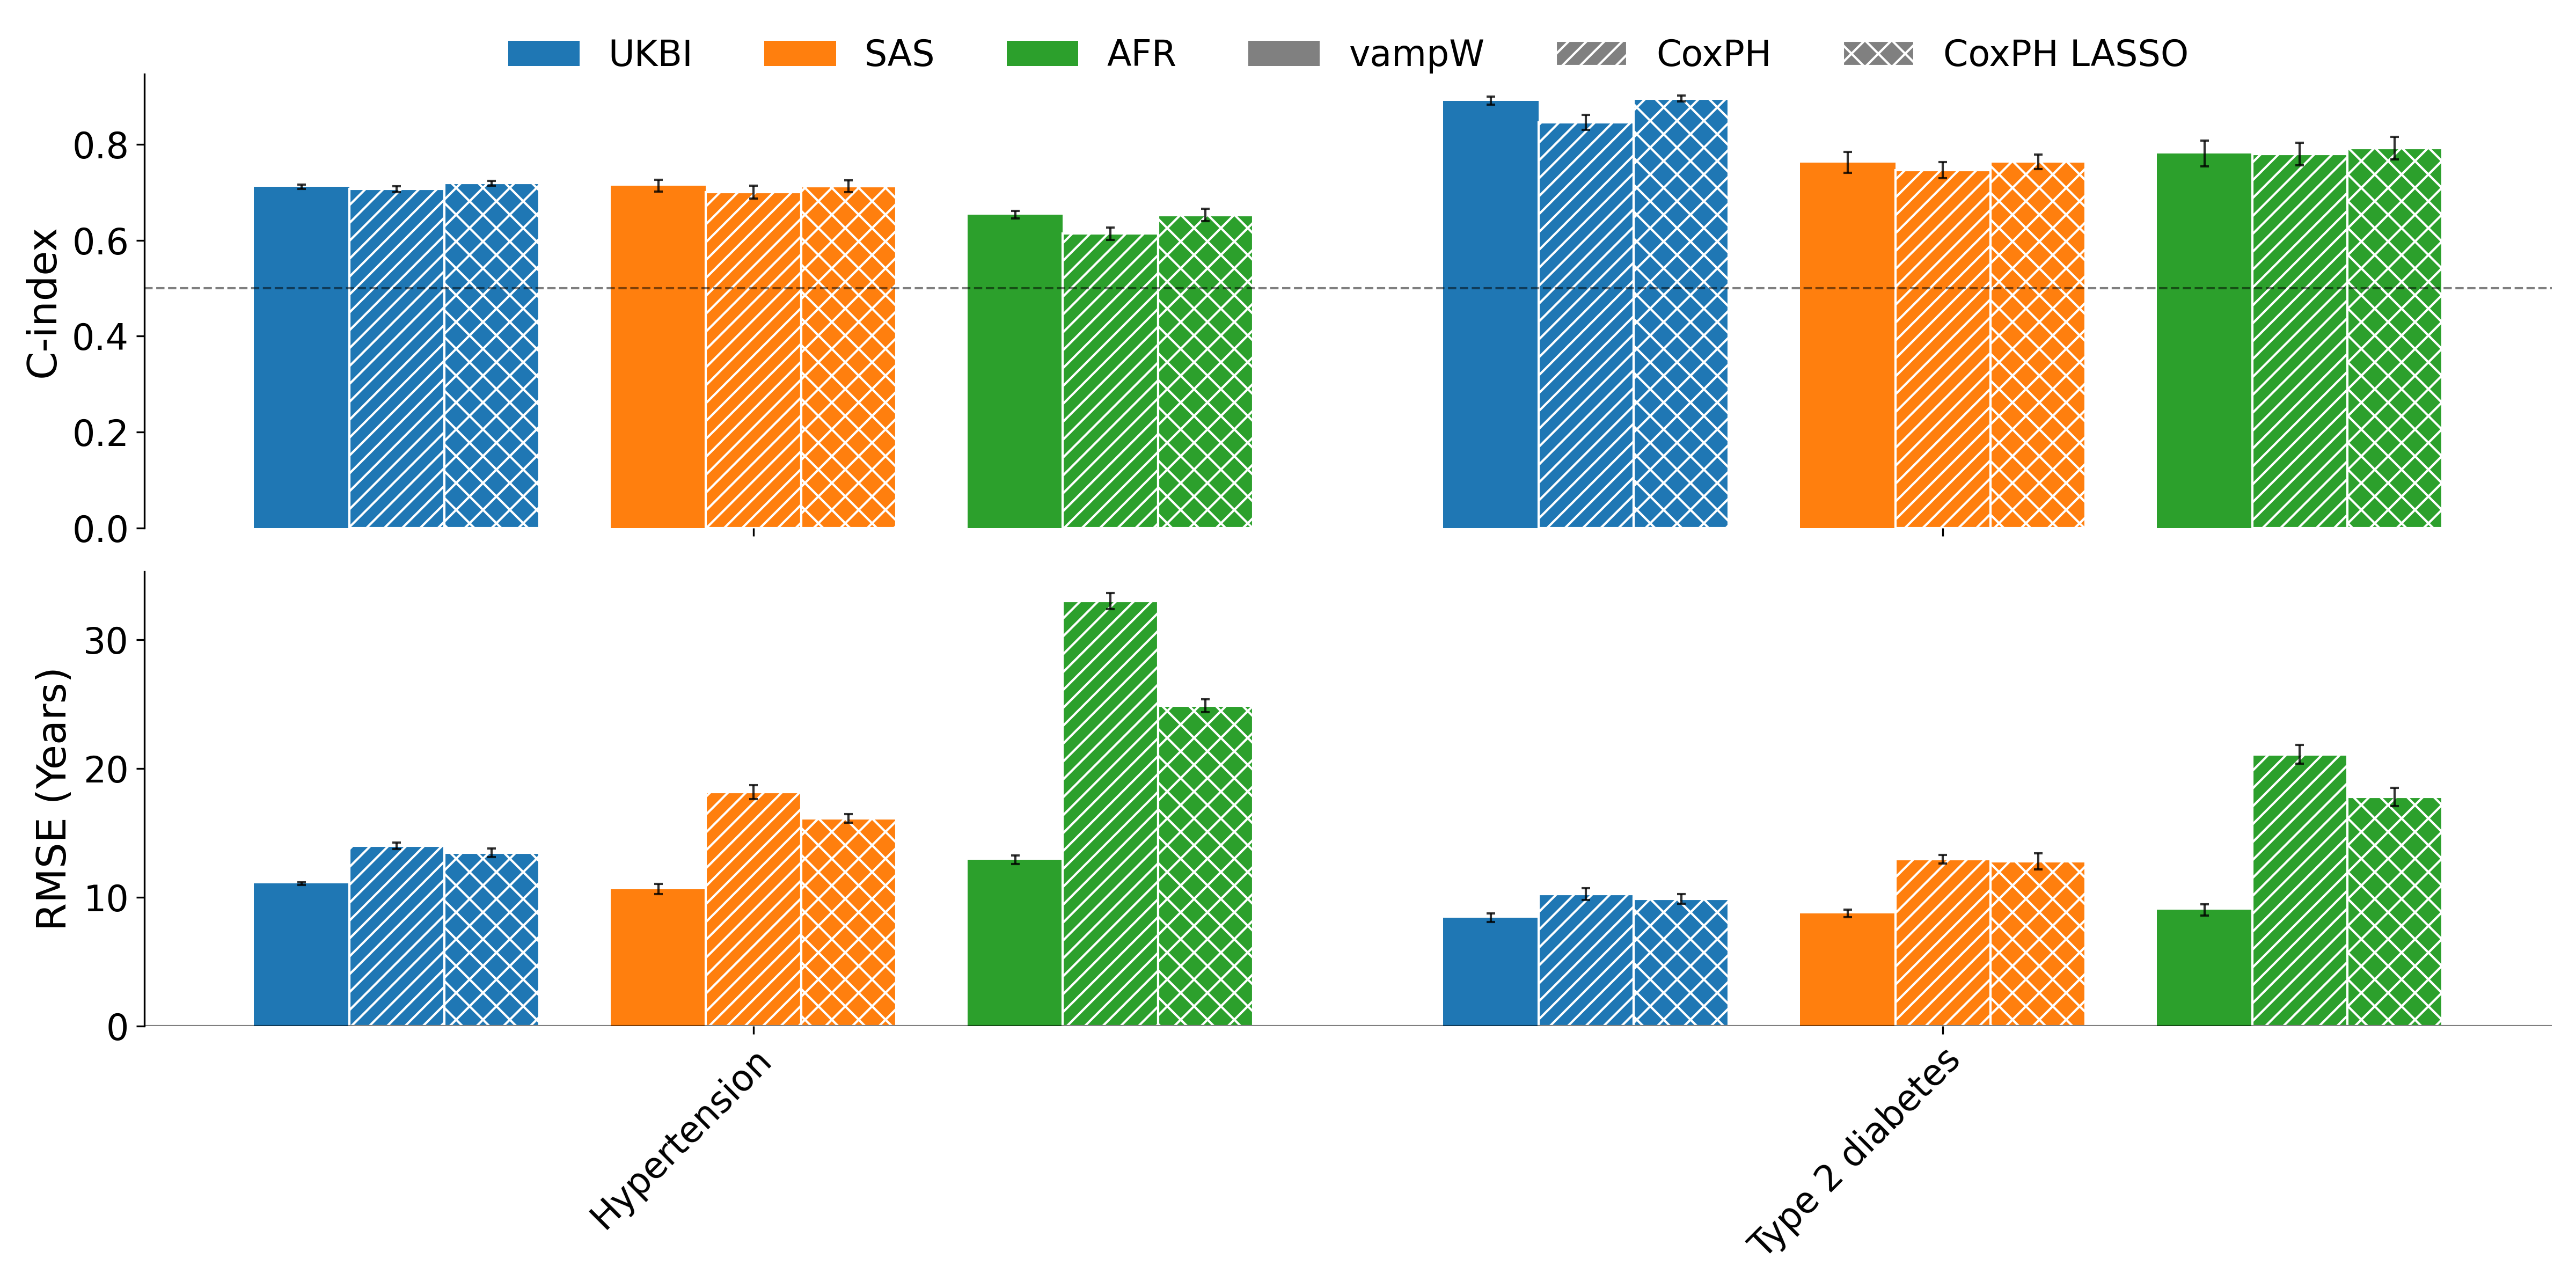
\includegraphics[width=\linewidth]{figures/genetic_ancestry_exp_50_10.png}
    \end{center}
    \caption[Out-of-sample prediction performance across distinct genetic ancestries]{\textbf{Out-of-sample prediction performance across distinct genetic ancestries.} We evaluate the predictive performance of vampW (solid bars), the standard CoxPH model (diagonal hatch lines), and CoxPH LASSO (cross hatch lines) across Hypertension and Type 2 diabetes traits from the UK Biobank. Results are stratified by genetic ancestry: British or Irish (UKBI, blue), South Asian (SAS, orange), and African (AFR, green). Performance is measured using the concordance index (C-index, top panel) and root mean squared error (RMSE in years, bottom panel). Phenotypic traits were included only if at least one minority ancestry group (SAS or AFR) contained a minimum of 200 total cases, ensuring that the 50\% data splits retained at least 100 cases per split. The reported error bars represent the standard deviation across 10 splits, with each split evaluating a random 50\% subsample of the dataset. We note that polygenic risk scores created by vampW are transferable to minority populations in the cohort; vampW exhibits similar C-index performance to Cox LASSO and outperforms the joint standard Cox model, while outperforming both competitor models in terms of the RMSE metric.}
\label{fig:genetic_ancestry_exp_50_10}
\end{figure}

\clearpage

\begin{figure}[H]
    \begin{center}
        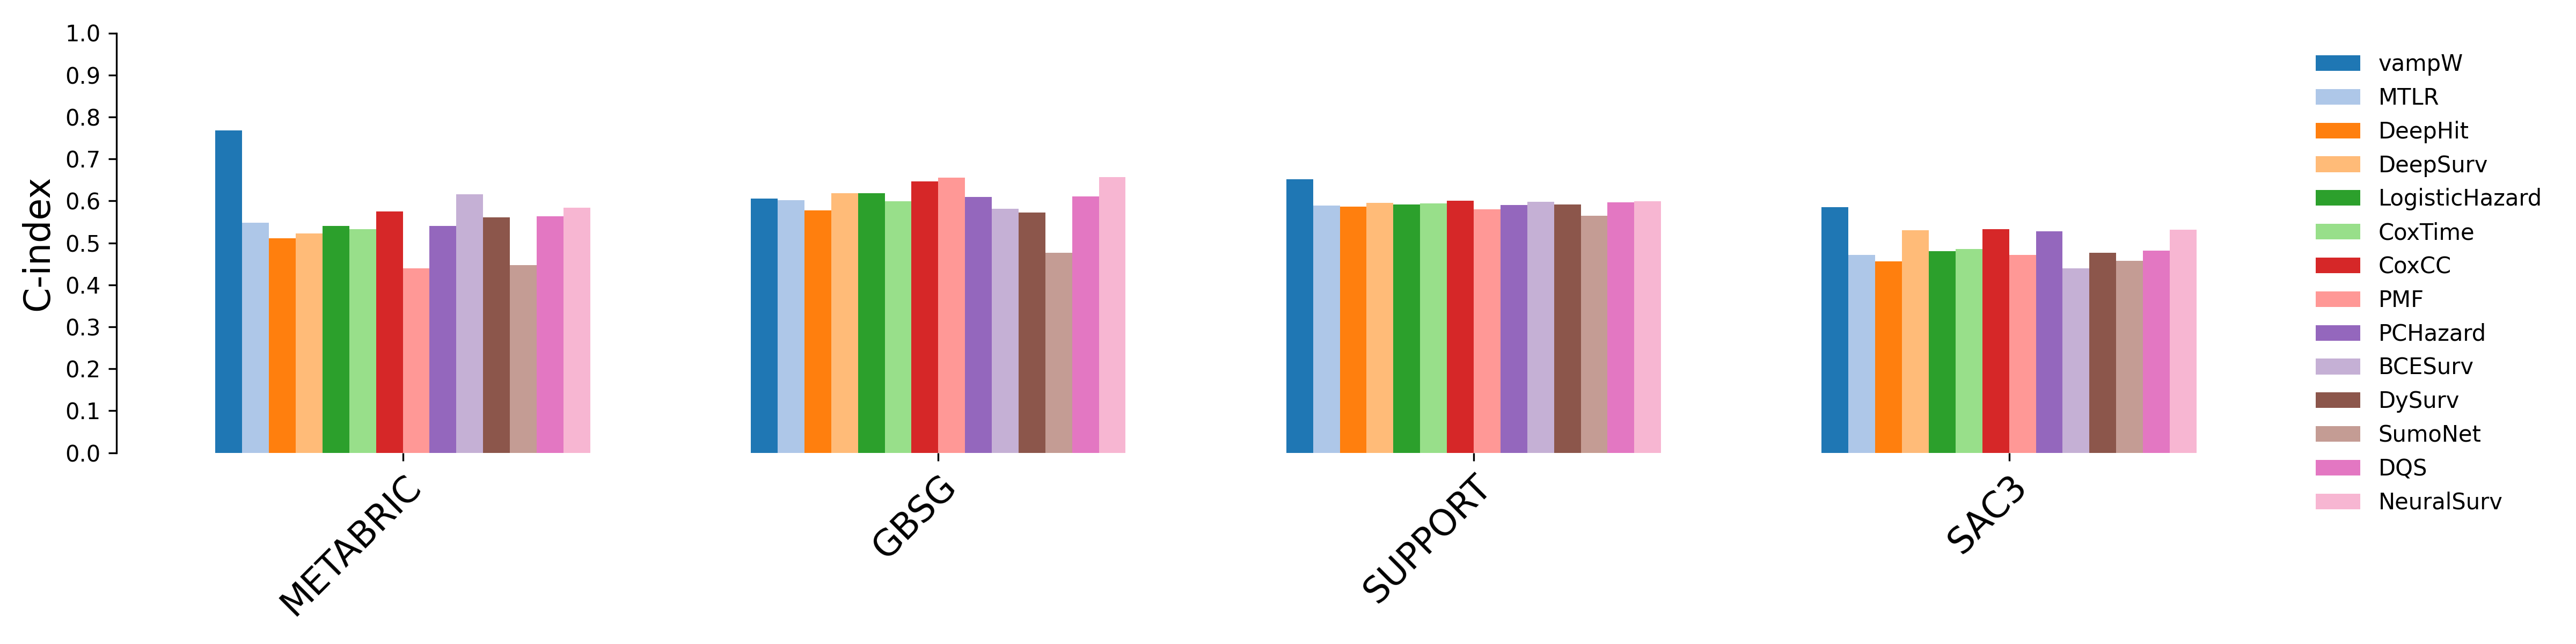
\includegraphics[width=\linewidth]{figures/deep_benchmark.png}
    \end{center}
    \caption[Out-of-sample performance comparison in terms of the Concordance index for vampW and deep learning methods]{\textbf{Out-of-sample performance comparison in terms of the Concordance index for vampW and deep learning methods.}
We compare predictions of vampW with common deep learning methods on several widely used survival benchmarking datasets, namely METABRIC, GBSG, SUPPORT, and SAC3. The benchmarking results for deep learning are reported in a recent NeuralSurv study \cite{monod_neuralsurv_2025}, which addresses prediction in data-scarce regimes. vampW outperforms all deep learning methods on METABRIC, SUPPORT, and SAC3 datasets, and outperforms 6 out of 13 benchmarking methods on the GBSG dataset.}
\label{fig:deep_benchmark}
\end{figure}

% \clearpage 


% \begin{figure}[H]
% \label{fig:vampw_age_corr}
%     \begin{center}
%         \includegraphics[width=\linewidth]{figures/real_vampw_cov_exp.png}
%     \end{center}
%     \caption{
%     \changed{\jakub{Figure added for consideration of whether to include it.}\textbf{Out-of-sample performance of vampW across two different approaches to age covariate adjustment.} We evaluate the out-of-sample C-index and Brier score at the 75\% time point for vampW, adjusting for age using either a linear model (solid color) or an exponential model (hatched color).}}
% \end{figure}

% \clearpage

% \begin{figure}[H]
% \label{fig:vampw_age_corr_disc}
%     \begin{center}
%         \includegraphics[width=\linewidth]{figures/real_vampw_disc.png}
%     \end{center}
%     \caption{
%     \changed{\jakub{Figure added for consideration of whether to include it.}\textbf{Number of vampW discoveries across different age correction approaches.} We plot number of significant proteomic markers above PIP threshold of 95\% for vampW, correcting for age using either a linear model (solid color) or an exponential model (hatched color). Here, we select the best iteration based on the highest C-index on the training data after several warm-up iterations. As the model in the exponentially corrected analysis stabilizes in later iterations, we use a longer warm-up period of 10 iterations, compared with 5 iterations in the linear approach.}}
% \end{figure}

\clearpage

% \section{Supplementary Note}
%\textbf{
\section{Details on denoiser for Weibull link function}
\label{sec:sup1}


We assume observations are independent, allowing for component-wise Maximum A Posteriori estimation. Proceeding with the construction of an age-at-onset denoiser for individual $i$, we express the posterior as follows, excluding terms independent of $z_i$:

\begin{equation}
    \begin{split}
    \arg \max_{z_i} \bigg \{ & \exp \bigg ( - \alpha z_i - y_i^{\alpha} \cdot \exp(-\alpha (\mu + z_i) - K) \bigg ) \\
    & \cdot \exp \bigg (-\frac{(z_i-p_{1, i})^2 \cdot \tau_1}{2} \bigg ) \bigg \}.
    \end{split} 
\end{equation}
Let us define $g_z: \mathbb{R} \to \mathbb{R}$ as
\begin{align}
    g_z(z_i) = -\alpha z_i - y_i^\alpha \cdot e^{-\alpha(\mu_i+z_i) - K} - \frac{(z_i-p_{1, i})^2 \cdot \tau_1}{2}.
\end{align}
Then, taking the derivative with respect to $z_i$, one obtains
\begin{equation}
     -\alpha + \alpha e^{-\alpha (\mu_i + z_i) - K} \cdot y^\alpha - \tau_{1}(z_i-p_1) = 0,
\end{equation}
which can be solved using fixed-point iterations. In addition, we note that
\begin{align}
 g_z''(z_i) = -\alpha^2 \cdot y_i^\alpha \cdot e^{-\alpha(\mu_i+z_i)-K} - \tau_1 < 0, \quad \text{for all } z_i,
\end{align}
and, hence, $g$ is a strictly concave function (see a visualization in Supplementary Figure \ref{fig:enter-label}).

\begin{figure}[!ht]
    \centering
    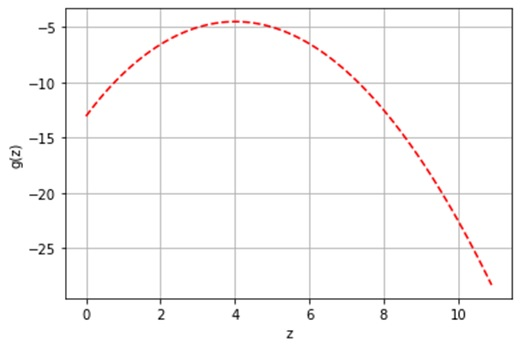
\includegraphics[width=0.44\linewidth]{figures/gz_weibull.jpg}
    \caption[Visualization of a function $g_z(z_i)$]{Visualization of a function $g_z(z_i)$ for $\alpha = 1, \tau_1 = 1, p = 5, \mu_i = 0, y_i = 1$}
    \label{fig:enter-label}
\end{figure}
Furthermore, by invoking the Implicit Function Theorem, we can compute the derivative of the denoiser as
\begin{align}
    \frac{dz}{dp_1} = \frac{\tau_1}{\tau_1 + \alpha^2 y_i^\alpha \cdot e^{-\alpha(\mu_i+z_i) - K}}.
\end{align}

\section{Details on EM hyperparameter updates}
\label{sec:sup3}

We %In this section, we 
present the derivation of the expectation-maximization update formulae for the hyperparameters $\mu$ and $\alpha$ under the Weibull model for non-censored phenotypic outcomes. We define the E-step and M-step of the EM algorithm at iteration $t$ of vampW in the following way:
\begin{enumerate}
    \item \underline{E-step}: The approximation of the posterior distribution typical for E-steps happens implicitly in VAMP-type algorithms, where the following
    approximate posterior probability distribution for the genetic component, $\bm{z} = \bm{X} \bm{\beta}$,  is obtained:
    \begin{align}
        b^{(t)}(\bm{z}) = \mathcal{N}(\bm{z}; \bm{\hat{z}_{2t}}^{(t)}, \bm{I}_N / \xi^{(t)}).
    \end{align}
    \item \underline{M-step}: We aim to maximize the evidence likelihood over $\mu$ and $\alpha$
    \begin{align}
        (\alpha^{(t+1)}, \mu^{(t+1)}) = \text{argmax}_{\mu, \alpha} \{ L^{(t)}(\mu, \alpha) \},
    \end{align}
    where we define 
    \begin{align}
        \begin{split}
        L^{(t)}(\mu, \alpha) & = \sum_{i=1}^N \int b_i^{(t)}(z_i) \cdot \log p(y_i|z_i, \alpha, \mu) dz_i \\
        & \quad = \sum_{i=1}^N \int \mathcal{N}(z_i; \hat{z}_i^{(t)}, 1 / \xi^{(t)}) \cdot \log p(y_i|z_i, \alpha, \mu) dz_i.
        \end{split}
    \end{align}
Here, $b_i^{(t)}(z_i)$ is the marginal distribution of the $i$-th component of $\bm{z}$ obtained from $b^{(t)}(\bm{z})$ and $\mathcal{N}(x; \mu, \sigma^2)$ denotes the probability density function of a Gaussian with mean $\mu$ and variance $\sigma^2$ evaluated at $x$.
    Furthermore, note that
    \begin{align}
        \begin{split}
        \log p(y_i|z_i, \alpha, \mu) & = \log(\alpha) + \alpha(\log y_i - \mu - z_i) - K \\
        & \quad - e^{\alpha(\log y_i - \mu - z_i) - K}.
        \end{split}
    \end{align}
\end{enumerate}
\underline{\textbf{Update formula for} $\alpha$:} \newline \newline
By taking the derivative of $L(\mu, \alpha)$ with respect to $\alpha$ and equating to zero we obtain:
\begin{align}
    \begin{split}
    \frac{\partial L^{(t)}(\mu, \alpha)}{\partial \alpha} = 0 & = \sum_{i=1}^N \int \mathcal{N}(z_i; \hat{z}^{(t)}, 1 / \xi^{(t)}) \cdot \left\{\frac{1}{\alpha} + \left(\log y_i - \mu - z_i\right) \right. \\
    & \qquad \left. \cdot \left[1 - e^{\alpha\left(\log y_i - \mu - z_i\right) - K}\right]\right\} dz_i.
    \end{split} 
\end{align}
Separating the term in brackets results in
\begin{align}
    \begin{split}
     & \sum_{i=1}^N \bigg [\frac{1}{\alpha} + \log y_i - \mu - \hat{z}_i^{(t)} \bigg ] \\
     &=
     \frac{N}{\alpha} + \sum_{i=1}^N [\log y_i - \mu - \hat{z}_i^{(t)}]  \\ 
     &= \sum_{i=1}^N \mathcal{N}(z_i; \hat{z}_i^{(t)}, 1 / \xi^{(t)}) \cdot (\log y_i - \mu - z_i) \cdot e^{\alpha(\log y_i - \mu - z_i) - K} dz_i \\
    &= \sum_{i=1}^N \int \mathcal{N}(\log y_i - \mu - \phi_i; \hat{z}_i^{(t)}; 1/\xi^{(t)}) \cdot \phi_i \cdot e^{\alpha \phi_i - K} d \phi_i \\
    &= e^{-K} \cdot \sum_{i=1}^N \exp(\alpha (\log y_i - \mu - \hat{z}_i^{(t)}) + \frac{\alpha^2}{2 \xi^{(t)}}) \\
    & \qquad \cdot \bigg ( (\log y_i - \mu - \hat{z}_i^{(t)}) + \frac{\alpha}{\xi^{(t)}} \bigg ).
    \end{split}
\end{align}
Finally, we define $f_{i}(\alpha) := e^{a_i \alpha + b \alpha^2 / 2} \cdot (a_i + \alpha b)$, where $a_i = \log y_i - \mu - {\hat{z}_i}^{(t)}$ and $b = \frac{1}{\xi^{(t)}}$. It follows that
\begin{align}
    f'(\alpha) = e^{a \alpha + b \alpha^2 / 2} ( a^2 + b + 2 ab \alpha + b^2 \alpha^2) > 0 \quad \text{ for all } \alpha > 0,
\end{align}
i.e. the function is strictly increasing in $\alpha$. This implies that the first derivative with respect to $\alpha$ of the likelihood function $L^{(t)}$ is
\begin{equation}
\frac{\partial L^{(t)}(\mu, \alpha)}{\partial \alpha} = \text{const} + \frac{N}{\alpha} - e^{-K} \sum_{i=1}^{N}f_i(\alpha).
\end{equation}
The second derivative is then given by

\begin{equation}
\frac{ \partial^2 L^{(t)}(\mu, \alpha)}{\partial^2 \alpha} = -\frac{N}{\alpha^2} - e^{-K} \sum_{i=1}^{N}f_i'(\alpha) < 0, \quad \mbox{for all } \alpha > 0.
\end{equation}
We thus have that the second derivative with respect to $\alpha$ is negative on the considered domain and hence the root of $\partial_{\alpha}L^{(t)}(\alpha, \mu) = 0$ attains a unique global maximum on the considered domain. We solve for the global maximizer $\alpha^*$ using numerical methods (SciPy optimize).
\newline
\newline
\noindent \underline{\textbf{Update formula for} $\mu$:} 
\newline 

\noindent Similarly, by taking the partial derivative of $L^{(t)}(\mu, \alpha)$ with respect to $\mu$ and equating it to zero, we obtain
\begin{align}
    \frac{\partial L^{(t)}(\mu, \alpha)}{\partial \mu} = 0 = \sum_{i=1}^N \int \mathcal{N}(z_i; \hat{z}_i^{(t)}, 1 / \xi^{(t)}) \cdot \alpha \cdot  [ e^{\alpha(\log y_i - \mu - z_i) - K} - 1] dz_i, 
\end{align}
where we use that 
\begin{align}
\frac{\partial \log p(y_i|z_i, \alpha, \mu)}{\partial \mu}= -\alpha + \alpha e^{\alpha(\log y_i - \mu - z_i) - K}.
\end{align}

By separating the term in brackets it follows that
\begin{align}
    \begin{split}
0 & = \alpha \sum_{i=1}^{n} \int \mathcal{N} \bigg (z_i; \hat{z}_i^{(t)}, \frac{1}{\xi^{(t)}} \bigg ) e^{\alpha(\log y_i - \mu - z_i) - K} dz_i \\
& \qquad - \alpha \sum_{i=1}^{n} \int \mathcal{N} \bigg (z_i; \hat{z}_i^{(t)}, \frac{1}{\xi^{(t)}} \bigg ) dz_i \\
& = \alpha \sum_{i=1}^{n} \exp \left( -K + \frac{\alpha^2}{2 \xi^{(t)}} + \alpha (\log y_i - \hat{z}_i^{(t)} - \mu) \right) \\
& \qquad - \alpha N \exp \left( -K + \frac{\alpha^2}{2 \xi^{(t)}} - \alpha \mu \right) \sum_{i=1}^{n} \exp \left( \alpha (\log y_i - \hat{z}_i^{(t)}) \right) \\
& = N -K + \frac{\alpha^2}{2 \xi^{(t)}} - \alpha \mu + \log \left( \sum_{i=1}^{n} \exp \left( \alpha (\log y_i - \hat{z}_i^{(t)}) \right) \right) \\
& = \log N.
    \end{split}
\end{align}
Hence, the update formula for $\mu$ satisfies
\begin{align}
\begin{split}
\mu & = \frac{-K}{\alpha} + \frac{\alpha}{2 \xi^{(t)}} \\
& \quad + \frac{1}{\alpha} \log \left( \sum_{i=1}^{n} \exp \left( \alpha (\log y_i - \hat{z}_i^{(t)}) \right) \right) - \frac{1}{\alpha} \log N.
\end{split}
\end{align}

Furthermore, the maximization problem at hand is concave: 
% We are considering maximization with respect to \(\alpha\) \marco{$\mu$?}:

% \[
% \text{argmax}_{\mu} \left\{ \sum_{i=1}^{N} \int \mathcal{N}(z_i; \hat{z}^{(t)}, 1 / \xi^{(t)}) \cdot \log p(y_i|z_i, \alpha, \mu) \, dz_i \right\} = \text{argmax}_{\mu} \{L(\mu)\}
% \]

% \[
% \frac{\partial L}{\partial \mu} = \exp \left( -K + \frac{\alpha^2}{2 \xi^{(t)}} - \alpha \mu \right) \sum_{i=1}^{n} \exp \left( \alpha (\log y_i - \hat{z}_i^{(t)}) \right) - N
% \]
\begin{equation}
\begin{split}
\frac{\partial^2 L^{(t)}}{\partial \mu^2} & = - \alpha \exp \left( -K + \frac{\alpha^2}{2 \xi^{(t)}} - \alpha \mu \right) \\
& \qquad \sum_{i=1}^{n} \exp \left( \alpha (\log y_i - \hat{z}_i^{(t)}) \right) - N < 0 \quad \text{for all } \alpha > 0.
\end{split}
\end{equation}

Therefore, $\mu$ satisfying $\frac{\partial L^{(t)}}{\partial \mu} = 0$ attains the global maximum of $L^{(t)}(\mu)$. 
%\marco{I did not understand the point of a few formulas above so I have removed them. Please restore in case I misunderstood the argument.} % in terms of $\mu$.

\clearpage

\section{Details on non-linear MMSE handling right-censorship}
\label{sec:sup2}

\noindent 
\begin{lemma}
    Differentiating the function inside the optimization problem (\ref{formula:cenosring_opt_problem}) with respect to $\bm{\beta}$ and equating the result to zero yields 
    \begin{align}
    %\nabla_\beta \text{nll} = 
    \begin{split}
    & 2 \gamma_{2t} (\bm{\beta} - \bm{r}_{2t}) + 2 \tau_{2t} \bm{X}^\top(\bm{X}\beta - \bm{p}_{2t}) \\
    & \quad - \alpha \bm{X}_\mathcal{C}^\top h(\alpha(\log(\bm{y}_\mathcal{C}) - \mu - \bm{X}_\mathcal{C} \bm{\beta})-K)= 0,
    \end{split}
    \end{align}
    where $h:\mathbb{R} \to \mathbb{R}$ is the standard hazard function of the Gumbel model given by $h(x) = e^x$, and the notation h($\bm{v}$) with $\bm{v}\in \mathbb{R}^{N}$ denotes the component-wise application of the function $h$. Furthermore, the Onsager corrections for the denoiser and nonlinear MMSE step are equal to 
\begin{align}
    \begin{split}
    \alpha_{2t} & = \frac{2 \cdot \gamma_{2t} \cdot \text{Trace}([J_{\beta}F(\hat{\bm{\beta}}_{2t})]^{-1})}{P}
    \quad \text{and} \\
    \upsilon_{2t} & = \frac{2 \cdot \tau_{2t} \cdot \text{Trace}(\bm{X} \cdot [J_{\beta}F(\hat{\bm{\beta}}_{2t})]^{-1} \cdot \bm{X}^\top)}{N}.
    \end{split}
\end{align}
\end{lemma}

\begin{proof}
    Let us define the function $g: \mathbb{R}^P \to \mathbb{R}$ with
    \begin{align}
    g(\bm{\beta}) = - \sum_{i=1}^{N_{\mathcal C}} \log S(\alpha(\log(y_{c,i}) - \mu - (\bm{X}_\mathcal{C} \bm{\beta})_i) -K),
    \end{align}
    where $N_{\mathcal C}$ is the number of censored individuals in the study and $\bm{X}_{\mathcal C}$ is the design matrix corresponding to those individuals. By performing differentiation, it follows that
    \begin{align}
        \begin{split}
        \frac{\partial g(\bm{\beta})}{\partial \bm{\beta}_j} & = - \sum_{i=1}^{N_{\mathcal C}} \alpha \cdot h(\alpha(\log(y_{c,i}) - \mu - (\bm{X}_\mathcal{C} \bm{\beta})_i) - K) \cdot  (\bm{X}_{\mathcal C})_{i,j} \\ & = - \alpha \langle h(\alpha(\log(y_{c,i}) - \mu - (\bm{X}_\mathcal{C} \beta)_i) - K), (\bm{X}_{\mathcal C})_{:,j} \rangle.
        \end{split}
    \end{align}
    Hence,
    \begin{align}
        \nabla_{\bm{\beta}} g(\bm{\beta})  = - \alpha \cdot \bm{X}_{\mathcal C}^\top h(\alpha(\log(\bm{y}_\mathcal{C}) - \mu - \bm{X}_\mathcal{C} \bm{\beta}) - K).
    \end{align}
    Furthermore,
    \begin{align}
        \begin{split}
        \frac{\partial g(\bm{\beta})}{\partial \bm{\beta}_k \partial \bm{\beta}_j} & = \frac{\partial}{\partial \bm{\beta}_k} \bigg [ - \sum_{i=1}^{N_{\mathcal C}} \alpha \cdot h(\alpha(\log \bm{y}_\mathcal{C} - \mu - \bm{X}_\mathcal{C} \bm{\beta})-K) \cdot (\bm{X}_{\mathcal C})_{i,j} \bigg ] \\
        & = \alpha^2 \sum_{i=1}^{N_{\mathcal C}} h'(\alpha (\log y_{c,i} - \mu - (\bm{X}_\mathcal{C} \bm{\beta})_i) - K) \cdot (\bm{X}_{\mathcal C})_{i,j} \cdot (\bm{X}_{\mathcal C})_{i,k} \\
        & = \alpha^2 \langle h'(\alpha (\log y_{c,i} - \mu - (\bm{X}_\mathcal{C} \bm{\beta})_i) - K) \cdot (\bm{X}_{\mathcal C})_{:,j}, (\bm{X}_{\mathcal C})_{:,k} \rangle,
        \end{split}
    \end{align}
    with $h'(x) = e^x$.
    It directly follows that
    \begin{align}
        \nabla^2 g(\bm{\beta}) = \alpha^2 \bm{X}_\mathcal{C}^\top \text{Diag}(h'(\alpha(\log \bm{y}_\mathcal{C} - \mu - \bm{X}_\mathcal{C} \bm{\beta})-K)) \bm{X}_\mathcal{C}.
    \end{align}
    We now define $F:\mathbb{R}^P \to \mathbb{R}^P$ as
    \begin{align}
        F(\beta) = 2(\gamma_{2t}\bm{I} + \tau_{2t}\bm{X}^\top\bm{X}) \bm{\beta} - \alpha \bm{X}_\mathcal{C}^\top h(\alpha(\log(\bm{y_\mathcal{C}}) - \mu - \bm{X_\mathcal{C}} \bm{\beta})-K),
    \end{align}
    which means that a solution $\hat{\bm{\beta}}_{2t}$ to the optimization problem (\ref{formula:cenosring_opt_problem}) satisfies 
    
    \begin{align}
        \hat{\bm{\beta}}_{2t} = F^{-1}(2 \gamma_{2t} \bm{r}_{2t} + 2 \tau_{2t} \bm{X}^\top \bm{p}_{2t}).
    \end{align}
    Note that
    \begin{align}
        \begin{split}
        & \text{div}_{r_{2t}}( F^{-1}(2 \gamma_{2t} r_{2t} + 2 \tau_{2t} \bm{X}^\top \bm{p}_{2t}) ) \\
        & = \text{Trace}(J_{\beta}F^{-1}(2 \gamma_{2t} r_{2t} + 2 \tau_{2t} \bm{X}^\top \bm{p}_{2t})) \cdot 2 \gamma_{2t} \\
        & = \text{Trace}([J_{\beta}F(F^{-1}(2 \gamma_{2t} r_{2t} + 2 \tau_{2t} \bm{X}^\top \bm{p}_{2t}))]^{-1}) \cdot 2 \gamma_{2t} \\
        & = \text{Trace}([J_{\beta}F(\hat{\bm{\beta}}_{2t})]^{-1}) \cdot 2 \gamma_{2t},
        \end{split}
    \end{align}
    where 
    \begin{align}
        \begin{split}
        J_{\beta} F(\hat{\beta}_{2t}) & = 2(\gamma_{2t}I + \tau_{2t}\bm{X}^\top\bm{X}) + \nabla^2 g(\hat{\bm{\beta}}_{2t}) \\
        & = 2(\gamma_{2t}I + \tau_{2t}\bm{X}^\top\bm{X}) \\
        & \qquad + \alpha^2 \bm{X}_\mathcal{C}^\top \text{Diag}\big(h'(\alpha(\log \bm{y}_\mathcal{C} - \mu - \bm{X}_\mathcal{C} \hat{\bm{\beta}}_{2t})-K)\big) \bm{X}_\mathcal{C}.
        \end{split}
    \end{align}
    Finally, we conclude that % Onsager correction for $\bm{\beta}$-denosier is
    \begin{align}
        \alpha_{2t} = \frac{2 \cdot \gamma_{2t} \cdot \text{Trace}([J_{\beta}F(\hat{\bm{\beta}}_{2t})]^{-1})}{P}.
    \end{align}
    Similarly, we derive %now proceed to deriving the Onsager correction for $z$:
    \begin{align}
        \begin{split}
        & \text{div}_{p_{2t}}(\bm{X} F^{-1}(2 \gamma_{2t} \bm{r}_{2t} + 2 \tau_{2t} \bm{X}^\top \bm{p}_{2t}) ) \\
        & = \text{Trace}(\bm{X} J_{\beta}F^{-1}(2 \gamma_{2t} \bm{r}_{2t} + 2 \tau_{2t} \bm{X}^\top \bm{p}_{2t}) \cdot 2 \tau_{2t} \cdot \bm{X}^\top) \\
        & = \text{Trace}(\bm{X} [J_{\beta}F(F^{-1}(2 \gamma_{2t} \bm{r}_{2t} + 2 \tau_{2t} \bm{X}^\top \bm{p}_{2t}))]^{-1} \cdot 2 \tau_{2t} \cdot \bm{X}^\top) \\
        & = 2 \tau_{2t} \cdot \text{Trace}(\bm{X} \cdot [J_{\beta}F(\hat{\beta}_{2t})]^{-1} \cdot \bm{X}^\top),
        \end{split}
    \end{align}
    which gives the Onsager correction %
%    Finally, we conclude the Onsager correction for $z$:
    \begin{align}
        \upsilon_{2t} = \frac{2 \cdot \tau_{2t} \cdot \text{Trace}(\bm{X} \cdot [J_{\beta}F(\hat{\bm{\beta}}_{2t})]^{-1} \cdot \bm{X}^\top)}{N}.
    \end{align}
    \end{proof}

\clearpage

\section{Details on Weibull and ExpGamma outcomes} \label{sec:sup4}

For the Weibull model, %given the $\bm{\beta}$ vector is already drawn as described in Methods \ref{sec:methods_sim}, 
we calculate the scaling factor 
\begin{equation}
    c = \sqrt{\bigg (\frac{1}{\sigma^2_G} - 1 \bigg ) \cdot \frac{\text{Var}(\bm{X}\bm{\beta})}{\sigma^2_{w}}},
\end{equation}
where $\sigma^2_w=\pi^2/6$ is the variance of the Gumbel distribution. Then, we generate time-to-event phenotypes as:
\begin{equation}
    \log({\bm{y}}) = \mu + \bm{X}\bm{\beta} + c \cdot (\bm{w} + \kappa).
\end{equation}
This formulation means that, in the phenotype $\log(\bm{y})$, the targeted proportion of variance is explained by markers.

For ExpGamma-distributed phenotypes, we exploit the fact that if $x \sim \text{ExpGamma}(\kappa, \theta, \tilde{\mu})$, then $ax + b \sim \text{ExpGamma}(\kappa, a \theta, a \tilde{\mu} + b)$. Then, we rewrite the model as follows:
\begin{align}
    \log y_i = \mu + \bm{x}_i^\top \bm{\beta} + \theta(w_i - \psi^{(0)}(\kappa)), \quad w_i \sim \text{ExpGamma}(\kappa, 1, 0),
\end{align}
with shape parameter $\kappa$, scale parameter $\theta$, and location parameter $\mu$.  We note that
\begin{align}
    \begin{split}
    & \mathbb{E}[\log y_i] = \theta  \psi ^{(0)}(\kappa )+ \tilde{\mu}, \\
    & 
    \text{Var}[\log y_i] = \theta ^2 \psi ^{(1)}(\kappa ),
    \end{split}
\end{align} where $\psi^{(m)}(\cdot)$ stands for the polygamma function of order $m$. Using the parametrization
\begin{equation}
    \theta = \sqrt{\bigg (\frac{1}{\sigma^2_G} - 1 \bigg ) \cdot \frac{\text{Var}(\bm{X\beta}) }{ \psi^{(1)}(\kappa)}},
\end{equation}
we obtain the time-to-event phenotypic outcomes, with the desired proportion of variance explained by the simulated markers.

\clearpage


% The declaration follows Appendix C without a blank page and with a more compact
% heading, so that it fits on one page.
\begingroup
\renewcommand{\clearforchapter}{\clearpage}
\renewcommand*{\chapterheadstart}{}
\renewcommand*{\afterchapternum}{\par\nobreak\vskip 12pt}
\setlength{\afterchapskip}{20pt}
% \chapter{Declaration of the Use of Generative AI Tools}
\chapter{Declaration of the Use of Generative AI and AI Tools}

% I have used Gemini 3 Thinking and Gemini 3 Pro version for text writing assistance, mainly for improving the flow of the written text and correcting grammar mistakes. I would input it the content which I have written and ask it to rephrase the text to improve the flow and correct grammar mistakes, while ensuring that the scientific content is not changed. Finally, I have carefully reviewed the outputs from these tools to ensure that they accurately reflect my statements I wanted to state.

% During the research phase, I have used Gemini 3 Pro for for debugging purposes for performing simulation and implementing pipeline for vampW project. I have used it to help me identify and fix bugs in my code. However, I would revistit all the suggestion to make sure that they are correct and do not change the scientific content of my work.

% I acknowledge that I have informed myself about the capabilities and limitations of generative AI systems used and labeled AI-generated content wherever necessary. Furthermore, I confirm that I have verified the factual accuracy of the content and that I take responsibility for all information in the submitted work.

Google Gemini models (Gemini 3 Thinking and Gemini 3 Pro) were employed for writing assistance and software debugging in the course of writting this thesis and performing research. For writing, these tools were utilized to rephrase author-drafted content to improve structural flow, enhance clarity, and correct grammatical errors. During the research phase, Gemini 3 Pro served as a debugging assistant to help identify and resolve code errors for performing simulations and implementing the pipeline for the vampW project.

The decision to use these AI tools was made to increase efficiency in the troubleshooting process and to ensure high-quality academic communication which is complementing traditional proofreading and debugging methods. The extent of AI usage was limited to refining the readability of the text and expediting the software development pipeline.

Potential limitations, such as the risk of AI-introduced hallucinations were considered. These risks were mitigated by testing all implemented code suggestions and cross-referencing the AI-refined text against the original to ensure that the scientific message remained the same.

I acknowledge that I have informed myself about the capabilities and limitations of the generative AI systems used and that I have documented and labeled AI-assisted content to the best of my ability. Furthermore, I confirm that I have verified the factual accuracy of the content and that I take full responsibility and ownership for all information, code, and findings presented in this submitted work.
\endgroup

% Blank pages up to the back cover, which is the last page and a left-hand (even)
% page: fill up to an odd page, then the blank inside of the back cover.
\clearpage
\begingroup
\pagestyle{empty}
\ifodd\value{page}\else\null\clearpage\fi
\null
\clearpage
\endgroup
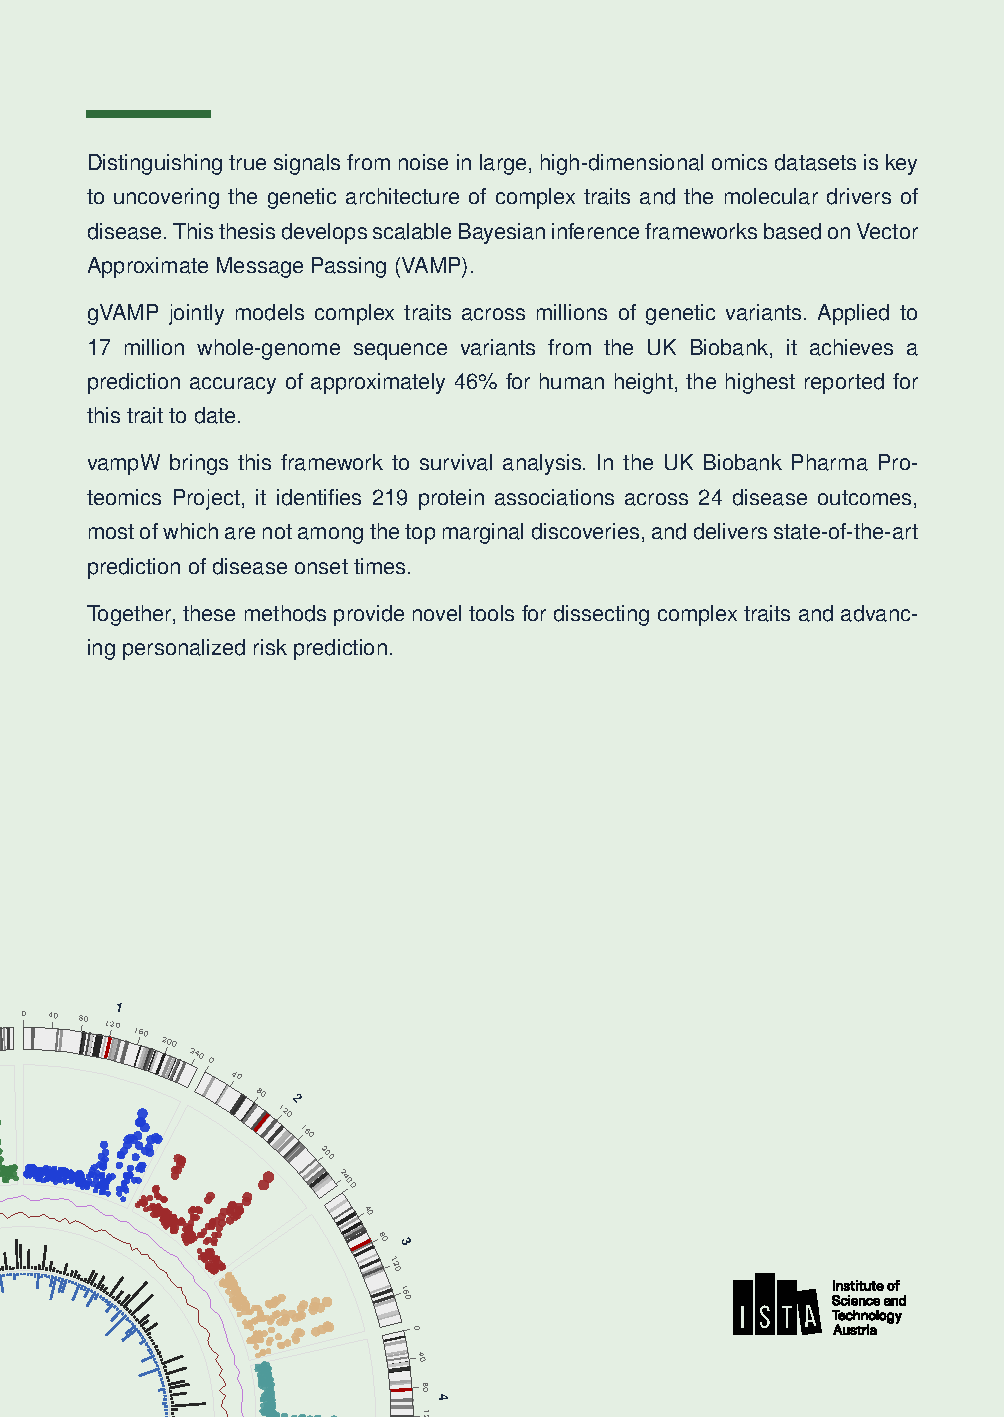
\includepdf[pages=1]{graphics/covers/back_light_green_170x240.pdf}

% \backmatter
% REMOVE THE FOLLOWING THREE LINES IN THE FINAL VERSION OF THE THESIS.
% \makeatletter\@todonotes@SetTodoListName{List of Todos}\makeatother % Set name of list of todos.
% \todototoc % Add the list of todos to the table of contents.
% \listoftodos % Add a list of all todos.

\end{document}